\documentclass[11pt,a4paper]{article}
\usepackage[margin=2.0cm]{geometry}
\usepackage{amsmath,amssymb,amsfonts}
\usepackage{booktabs}
\usepackage{graphicx}
\usepackage{hyperref}
\usepackage{float}
\usepackage{placeins}
\usepackage{caption}
\usepackage{subcaption}
\usepackage{listings}
\usepackage{xcolor}
\usepackage{enumitem}
\usepackage{tikz}
\usetikzlibrary{patterns, arrows, positioning}

\graphicspath{{report_figs/pred/}{report_figs/}{figures/}}

\definecolor{primary}{RGB}{16, 44, 87}
\definecolor{secondary}{RGB}{53, 95, 142}
\definecolor{codebg}{RGB}{248, 249, 250}
\definecolor{codegray}{RGB}{120, 120, 120}

\lstset{
  backgroundcolor=\color{codebg},
  basicstyle=\ttfamily\footnotesize,
  breaklines=true,
  breakatwhitespace=true,
  commentstyle=\color{codegray},
  frame=single,
  numbers=left,
  numbersep=5pt,
  numberstyle=\tiny\color{codegray},
  showstringspaces=false,
  tabsize=2
}

\hypersetup{
    colorlinks=true,
    linkcolor=primary,
    citecolor=primary,
    urlcolor=secondary,
    bookmarksnumbered=true,
    pdftitle={Prediction of Flow Field Using Machine Learning},
    pdfauthor={Divyansh Singh}
}

\title{
\includegraphics[height=2.2cm]{figures/iitk_logo_cropped.png}\\[1.0em]\LARGE\textbf{Prediction of Flow Field Using Machine Learning}}

\author{\textbf{Divyansh Singh}}
\date{}

\begin{document}
\maketitle

\begin{abstract}
Physics-informed neural networks (PINNs) are trained to predict developing internal flows in five configurations of increasing complexity: laminar flow between parallel plates (Stage 1), in a circular pipe (Stage 2) and in a rectangular duct of aspect ratio 2 (Stage 3), and turbulent flow in a channel (Stage 4) and in a pipe (Stage 5) at Re = $10^4$ to $1.2\times10^5$, modeled with the Reynolds-averaged Navier--Stokes equations and the Spalart--Allmaras turbulence model. A sixth stage, a turbulent rectangular duct, was started but not completed, and no results are reported for it. Each network is trained on reference solutions from a parabolic marching solver together with the governing equations, and is tested at Reynolds numbers outside its training set. The relative $L_2$ error of the streamwise velocity is 2.20\%--5.69\% for the laminar channel and pipe, 8.8\%--12.7\% for the laminar duct, and 0.36\%--0.58\% for the turbulent cases at the test Reynolds numbers. For the turbulent pipe, the predicted velocity profiles agree with Princeton Superpipe measurements to within 2.81\%--4.18\% relative $L_2$ error. Two weaknesses are documented. In the duct, the pressure error is 56.8\%--106.4\%; downstream of $x=1.5$ m the pressure gradient of the network is 0.22 to 0.38 times the reference gradient at Re = 50--100 and agrees within 4\% at Re = 500--600, and the reference solution contains an inlet pressure transient. In the turbulent channel the eddy-viscosity variable $\tilde\nu$ is almost zero (error above 99\%), whereas in the turbulent pipe it is partly recovered (error 47\%--80\%); the ratio of the turbulence-equation loss weight to the data weight is $4.9\times10^{-9}$ in the channel and $1.1\times10^{-3}$ in the pipe, a factor of about $2.3\times10^{5}$. At the end of training the data term carries 79\% of the weighted loss in the channel and 34\% in the pipe, so both turbulent networks are mainly data-driven. With 1\% of the reference data, adding the physics loss lowers the test error by about 31\% (channel) and 56\% (pipe); with all the data it changes nothing. These results come from single training runs, and no experiment isolates their causes.
\end{abstract}


\newpage
\tableofcontents
\newpage

% ==============================================================================
% SECTION 1: INTRODUCTION
% ==============================================================================

\section*{Nomenclature}
\addcontentsline{toc}{section}{Nomenclature}
\begin{table}[H]
\centering
\small
\resizebox{\linewidth}{!}{%
\begin{tabular}{lll}
\toprule
\textbf{Symbol} & \textbf{Meaning} & \textbf{Unit} \\
\midrule
$U_0, U_b$ & Inlet uniform velocity, cross-sectional bulk velocity & m/s \\
$U_{\mathrm{ref}}$ & Reference velocity: $U_0$ (Stages 1--2), $U_{\mathrm{mean}}$ (Stage 3), $U_b$ (Stages 4--5) & m/s \\
$p_{\mathrm{scale}}$ & Pressure scale for $p/\rho$: $0.5U_0^2$ (Stage 1), $32\nu U_0L/D^2$ (Stage 2), $0.5U_{\mathrm{ref}}^2L/D_h$ (Stage 3) & m$^2$/s$^2$ \\
$h, H, W$ & Channel half-height, duct height, duct width & m \\
$R, D$ & Pipe radius, pipe diameter ($D = 2R$) & m \\
$D_h, L$ & Hydraulic diameter ($4A/P$), conduit axial length & m \\
$\nu, \tilde{\nu}$ & Molecular kinematic viscosity, Spalart--Allmaras modified working variable & m$^2$/s \\
$\nu_t, \nu_{\mathrm{eff}}$ & Turbulent kinematic eddy viscosity ($\nu_t = \tilde{\nu} f_{v1}$), effective viscosity ($\nu + \nu_t$) & m$^2$/s \\
$u_\tau, y^+$ & Friction velocity ($\sqrt{\tau_w/\rho}$), inner wall coordinate ($y u_\tau / \nu$) & m/s, -- \\
$\mathrm{Re}_\tau, \eta$ & Friction Reynolds number ($u_\tau h/\nu$ or $u_\tau R/\nu$), dimensionless wall distance & -- \\
$d, C_f$ & Distance to closest solid wall, skin friction coefficient ($2\tau_w / \rho U_b^2$) & m, -- \\
$S, \tilde{S}$ & Vorticity magnitude, modified deformation magnitude in Spalart--Allmaras model & 1/s \\
$w_i, \mathcal{L}_i$ & Objective weight for loss term $i$, individual scalar loss residual $i$ & --, -- \\
$N_{\mathrm{data}}, N_{\mathrm{pde}}, N_{\mathrm{bc}}$ & Collocation points per iteration for data misfit, PDE residuals, boundary conditions & -- \\
\bottomrule
\end{tabular}%
}
\end{table}


\section{Introduction and Engineering Motivation}
\label{sec:intro}
Predicting the hydrodynamic development of internal flows in ducts, channels, and pipelines is central to fluid dynamics, thermal engineering, and piping network design. In this report, ``data'' means values of a reference numerical solution; only the Stage~5 validation uses measurements. As fluid enters a conduit with a uniform velocity profile, viscous wall shear retards near-wall fluid, generating growing boundary layers that merge downstream into a fully developed profile. Accurately resolving this development region is essential for predicting pressure drops, pumping power, and wall shear stresses.

Traditional computational approaches rely on spatial discretization: finite-difference marching schemes for parabolic entrance equations~\cite[Chs.~6--7, pp.~153--202]{hornbeck1973} or elliptic finite-volume solvers such as OpenFOAM. While effective, mesh-based techniques require separate computational grids for each geometric configuration and re-meshing across parametric operating sweeps. 

Physics-Informed Neural Networks (PINNs), pioneered by Raissi et al.~\cite[abstract, p.~1]{raissi2019} and extended to incompressible flows by Rao et al.~\cite[Sec.~2, p.~2]{rao2020}, reformulate boundary value problems as continuous function approximation tasks. A deep neural network takes continuous spatial coordinates and operational parameters (such as the Reynolds number $\mathrm{Re}$) as inputs and outputs the primary flow variables $(u, v, w, p)$. By computing spatial derivatives using Automatic Differentiation (Autograd), the governing differential equations are incorporated directly into the optimization loss function. Classical boundary layer theory provides theoretical foundations for analyzing these entrance shear layers.

Recent literature has advanced PINN formulations for fluid dynamics across multiple configurations. Jin et al.~\cite[abstract, p.~1]{jin2021} developed NSFnets for incompressible laminar and turbulent flows, Cai et al.~\cite[abstract, p.~1]{cai2021} reviewed physics-informed deep learning methodologies for fluid mechanics, and Eivazi et al.~\cite[abstract, p.~1]{eivazi2022} applied PINNs to solve RANS equations for incompressible turbulent flows. Concurrently, theoretical analyses have examined optimization challenges: Wang et al.~\cite[abstract, p.~1]{wang2022ntk} analyzed training dynamics and failure modes through neural tangent kernels, while Krishnapriyan et al.~\cite[abstract, p.~1]{krishnapriyan2021} characterized failure modes in differential equations with convection, reaction, and diffusion operators. In contrast to isolated forward or inverse benchmarks on fixed geometries, the present work systematically investigates hydrodynamic entrance development across parametric Reynolds-number ranges, geometry transfer across channels, pipes, and 3D ducts, and conducts an audit of loss-weighting failures in pressure-drop and turbulence closure.

\begin{figure}[H]
\centering
\hyphenpenalty=10000
\exhyphenpenalty=10000
\resizebox{\linewidth}{!}{%
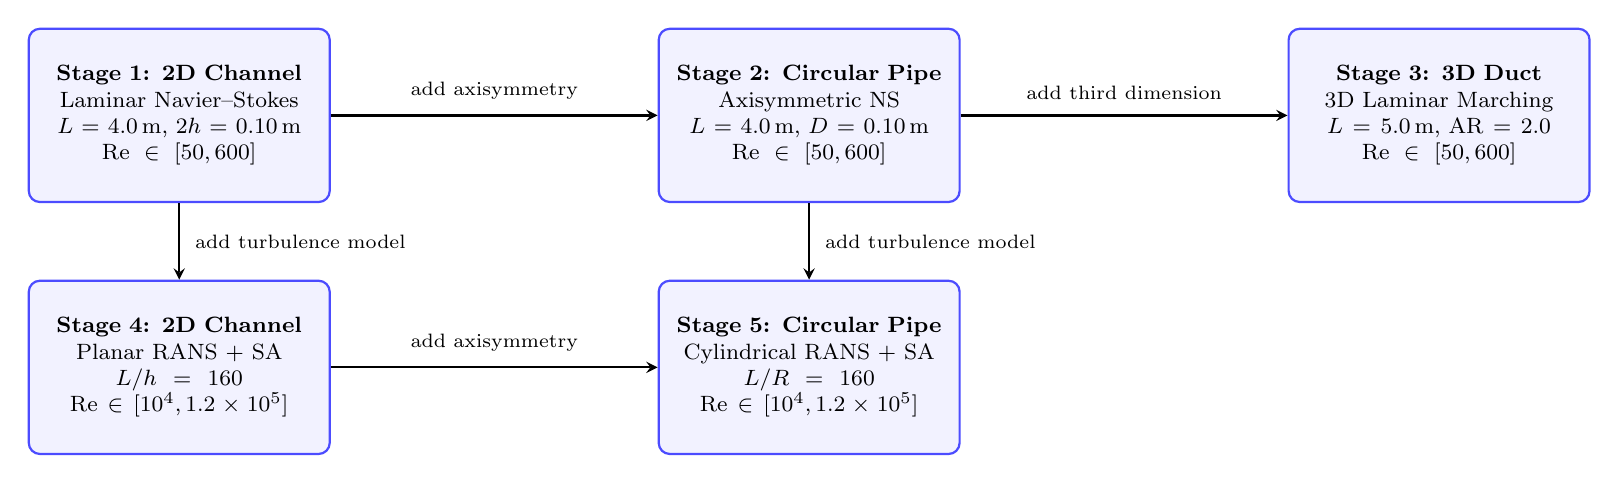
\begin{tikzpicture}[
    stage/.style={rectangle, draw=blue!70, fill=blue!5, thick, rounded corners, text width=3.4cm, minimum height=2.2cm, align=center, font=\footnotesize, inner sep=6pt},
    arrow/.style={thick, ->, >=stealth}]
    % Row 1: Laminar (Re = 50--600)
    \node (s1) at (0, 0) [stage] {\textbf{Stage 1: 2D Channel}\\Laminar Navier--Stokes\\$L=4.0\,\text{m},\,2h=0.10\,\text{m}$\\$\mathrm{Re} \in [50, 600]$};
    \node (s2) at (8.0, 0) [stage] {\textbf{Stage 2: Circular Pipe}\\Axisymmetric NS\\$L=4.0\,\text{m},\,D=0.10\,\text{m}$\\$\mathrm{Re} \in [50, 600]$};
    \node (s3) at (16.0, 0) [stage] {\textbf{Stage 3: 3D Duct}\\3D Laminar Marching\\$L=5.0\,\text{m},\,\mathrm{AR}=2.0$\\$\mathrm{Re} \in [50, 600]$};
    
    % Row 2: Turbulent (Re = 10^4--1.2*10^5)
    \node (s4) at (0, -3.2) [stage] {\textbf{Stage 4: 2D Channel}\\Planar RANS + SA\\$L/h=160$\\$\mathrm{Re} \in [10^4, 1.2\times 10^5]$};
    \node (s5) at (8.0, -3.2) [stage] {\textbf{Stage 5: Circular Pipe}\\Cylindrical RANS + SA\\$L/R=160$\\$\mathrm{Re} \in [10^4, 1.2\times 10^5]$};
    
    % Horizontal arrows
    \draw [arrow] (s1) -- node[midway, above=2pt, font=\scriptsize] {add axisymmetry} (s2);
    \draw [arrow] (s2) -- node[midway, above=2pt, font=\scriptsize] {add third dimension} (s3);
    \draw [arrow] (s4) -- node[midway, above=2pt, font=\scriptsize] {add axisymmetry} (s5);
    
    % Vertical arrows
    \draw [arrow] (s1) -- node[midway, right=2pt, font=\scriptsize] {add turbulence model} (s4);
    \draw [arrow] (s2) -- node[midway, right=2pt, font=\scriptsize] {add turbulence model} (s5);
\end{tikzpicture}%
}
\caption{The five-stage pipeline progression across cross-sectional geometries and flow physics regimes.}
\label{fig:pipeline_flowchart}
\end{figure}

Figure~\ref{fig:pipeline_flowchart} illustrates the logical progression investigated in this report:
\begin{enumerate}[leftmargin=2em]
    \item \textbf{Stage 1 (Laminar Plane Channel):} 2D Navier--Stokes entrance flow between parallel plates ($L=4.0\,\text{m}, h=0.05\,\text{m}, D_h=0.20\,\text{m}$, $\mathrm{Re} \in [50, 600]$).
    \item \textbf{Stage 2 (Laminar Axisymmetric Pipe):} Circular pipe entrance flow ($L=4.0\,\text{m}, R=0.05\,\text{m}, D=0.10\,\text{m}$, $\mathrm{Re} \in [50, 600]$), resolving the coordinate axis singularity at $r=0$.
    \item \textbf{Stage 3 (Laminar 3D Rectangular Duct):} Rectangular passage ($L=5.0\,\text{m}$, $H=0.10\,\text{m}$, $W=0.20\,\text{m}$, aspect ratio $\mathrm{AR}=2.0$, $D_h=0.1333\,\text{m}$), incorporating two-dimensional wall shear interactions.
    \item \textbf{Stage 4 (Turbulent Developing Channel):} 2D turbulent channel flow ($L/h = 160$, $\mathrm{Re} \in [10^4, 1.2\times 10^5]$) governed by the elliptic RANS equations with Spalart--Allmaras eddy viscosity transport~\cite[Sec.~2.1, p.~2]{allmaras2012}.
    \item \textbf{Stage 5 (Turbulent Developing Pipe):} Cylindrical RANS+SA pipe flow ($L/R = 160$, $\mathrm{Re} \in [10^4, 1.2\times 10^5]$), benchmarked against high-Reynolds-number experimental data from the Princeton Superpipe~\cite{superpipe_data}.
\end{enumerate}

Quantitative metrics were computed from the saved checkpoint files and the evaluation scripts listed in Appendix~\ref{sec:app_tables}.

% ==============================================================================
% SECTION 2: FOUNDATIONAL CONCEPTS
% ==============================================================================
\section{Foundational Concepts for Fluid Dynamicists}
\label{sec:foundations}
This section defines the flow configurations, machine-learning principles, evaluation metrics, and operational terminology used throughout the report.

\subsection{Fluid Mechanics Concepts}
\begin{itemize}[leftmargin=1.5em]
    \item \textbf{Reynolds Number ($\mathrm{Re}$):} The ratio of convective inertial forces to viscous friction forces ($\mathrm{Re} = U D_h / \nu$). It governs the relative importance of viscous dissipation compared to fluid momentum.
    \item \textbf{Laminar vs.\ Turbulent Flow:} Laminar flow is orderly and layered, where fluid parcels slide smoothly past each other without cross-stream mixing. Turbulent flow is characterized by chaotic, three-dimensional velocity fluctuations, eddy cascade, and rapid transverse momentum exchange.
    \item \textbf{Hydrodynamic Entrance Length ($L_e$):} The axial distance from the inlet required for viscous boundary layers growing from opposite walls to merge across the core, transforming a flat inlet velocity profile into an invariant fully developed profile.
    \item \textbf{Poiseuille and Hagen--Poiseuille Flow:} The exact parabolic velocity profile that develops in fully developed laminar flow between parallel plates ($u_{\max} = 1.5 U_0$) or in circular pipes ($u_{\max} = 2.0 U_0$).
    \item \textbf{Hydraulic Diameter ($D_h$):} A characteristic length scale defined as $D_h = 4A/P$, where $A$ is the cross-sectional flow area and $P$ is the wetted perimeter, allowing non-circular conduits to be compared to circular pipes.
    \item \textbf{Reynolds-Averaged Navier--Stokes (RANS):} A statistical framework decomposing instantaneous velocity into a time-averaged mean and a turbulent fluctuation ($\mathbf{u} = \overline{\mathbf{u}} + \mathbf{u}'$), yielding equations for the mean flow that contain unclosed correlation terms.
    \item \textbf{Reynolds Stress Tensor ($-\rho \overline{u_i' u_j'}$):} Apparent turbulent stresses appearing in the RANS equations representing the net cross-stream momentum transport caused by velocity fluctuations.
    \item \textbf{Boussinesq Eddy Viscosity Hypothesis:} An engineering approximation modeling Reynolds stresses by analogy to molecular viscous stresses: $-\rho \overline{u_i' u_j'} = \mu_t (\partial \overline{u}_i/\partial x_j + \partial \overline{u}_j/\partial x_i) - \frac{2}{3}\rho k \delta_{ij}$, where $\mu_t = \rho \nu_t$ is the turbulent eddy viscosity.
    \item \textbf{Spalart--Allmaras (SA) Model:} A one-equation turbulence model solving a transport equation for a modified kinematic eddy viscosity $\tilde{\nu}$, accounting for turbulent production near walls, viscous destruction, diffusion, and cross-diffusion~\cite[Sec.~2.1, p.~2]{allmaras2012}.
    \item \textbf{Friction Velocity ($u_\tau$):} A characteristic turbulent velocity scale defined from the wall shear stress $\tau_w$: $u_\tau = \sqrt{\tau_w / \rho}$.
    \item \textbf{Dimensionless Wall Distance ($y^+$):} An inner-scaled spatial coordinate normalized by the viscous length scale: $y^+ = y u_\tau / \nu$. The viscous sublayer occupies $y^+ < 5$, and the logarithmic overlap region spans $30 < y^+ < 300$.
    \item \textbf{Law of the Wall:} The universal logarithmic velocity distribution in wall-bounded turbulent shear flows: $u^+ = u / u_\tau = \frac{1}{\kappa} \ln y^+ + B$, where $\kappa \approx 0.41$ and $B \approx 5.0$.
    \item \textbf{Skin Friction Coefficient ($C_f$):} Dimensionless wall shear stress defined as $C_f = 2\tau_w / (\rho U_b^2)$, characterizing the frictional resistance of the conduit walls.
\end{itemize}


\paragraph{Mathematical Distinction Between Network and Reference Formulations.}
\label{sec:elliptic_vs_parabolic}
A methodological distinction exists between the equations satisfied by the neural network and those solved by the numerical reference code:
\begin{enumerate}[label=(\roman*)]
\item \textbf{Full Navier--Stokes system solved by the PINN:} The neural network is trained on the full, steady, incompressible Navier--Stokes equations (or the full elliptic Reynolds-averaged equations in turbulent regimes), retaining both streamwise diffusion ($\partial^2/\partial x^2$) and cross-stream pressure gradients ($\partial p/\partial y$ or $\partial P/\partial r$). A mesh-free network incorporates these terms via automatic differentiation without geometric meshing. The full elliptic formulation makes no boundary-layer assumption, remaining valid in the entrance region ($x \to 0$) where axial velocity gradients are steepest.
\item \textbf{Parabolic marching reference solver:} The reference data are generated with implicit finite-difference marching schemes of Hornbeck type~\cite[Chs.~6--7, pp.~153--202]{hornbeck1973}. A marching solver produces a reference solution in seconds to minutes on a CPU. An elliptic solver (for example a finite-volume code) would solve the same equations as the network and would remove the mismatch; it was not used here (Sec.~\ref{sec:future}).
\item \textbf{Consequence and modeling limitation:} Because the marching solver neglects axial diffusion ($\partial^2 u/\partial x^2 \approx 0$) and sets the cross-stream pressure gradient to zero ($\partial p/\partial y = 0$), the network and reference solver solve different equations. A localized difference between the PINN prediction and the reference profile is expected near the conduit inlet ($x \lesssim 0.5\,D_h$), and the reference is not an exact solution of the elliptic system satisfied by the network.
\end{enumerate}


\subsection{Machine-Learning Terms and Design Principles}
\begin{itemize}[leftmargin=1.5em]
    \item \textbf{Neuron / Unit:} An elementary scalar processing node that computes an affine combination of its inputs followed by a non-linear activation function.
    \item \textbf{Layer:} A collection of parallel neurons operating at the same depth within the network hierarchy.
    \item \textbf{Multilayer Perceptron (MLP):} A feedforward neural network structured in successive layers of neurons. Each layer applies a linear matrix transformation plus an offset bias and passes the result through a non-linear activation function.
    \item \textbf{Weights ($W$) and Biases ($b$):} The trainable numerical parameters of the network. Weights scale input signals, while biases shift the activation threshold.
    \item \textbf{Activation Function ($\tanh$):} A smooth mapping ($\tanh(z) = (e^z - e^{-z})/(e^z + e^{-z})$). Because it possesses continuous derivatives of all orders, $\tanh$ enables exact automatic differentiation of viscous diffusion terms ($\nabla^2 u$).
    \item \textbf{Xavier (Glorot) Initialization:} A technique for initializing weight matrices so that the variance of activations and backpropagated gradients remains constant across layers~\cite[Eq.~(12), p.~253]{glorot2010}, setting $\operatorname{Var}(W) = 2/(n_{\mathrm{in}} + n_{\mathrm{out}})$.
    \item \textbf{Collocation Point:} A discrete spatial coordinate $(x, y, [z])$ sampled in the fluid domain where differential equations are evaluated via automatic differentiation without requiring numerical mesh connectivity or reference data.
    \item \textbf{Automatic Differentiation (autograd):} A technique that evaluates exact derivatives of network outputs with respect to spatial inputs by applying the chain rule down to machine precision, avoiding finite-difference truncation error.
    \item \textbf{Soft vs.\ Hard Boundary Conditions:} Soft boundary conditions add penalty terms to the objective function, enforcing boundary values approximately. Hard boundary conditions enforce exact Dirichlet values by multiplying outputs by an analytical distance envelope (e.g., $u = g(y) \hat{u}$ where $g(0) = 0$).
    \item \textbf{Input and Output Normalization:} Rescaling raw coordinates (e.g., $x \in [0, 4]\,\text{m}$) and physical fields into standard compact ranges (e.g., $[-1, 1]$ or $[0, 1]$). Normalization ensures balanced gradient magnitudes across different spatial dimensions.
    \item \textbf{Composite Loss Function:} A single scalar objective minimized by the optimizer, formed as a weighted sum of data discrepancies, boundary penalties, and differential equation residuals: $\mathcal{L}_{\mathrm{total}} = \sum w_i \mathcal{L}_i$.
    \item \textbf{PDE Residual ($r$):} The algebraic evaluation of the governing differential operator applied to the network prediction; $r=0$ denotes exact satisfaction of the physical law.
    \item \textbf{Loss Weighting and Wang Gradient-Norm Weighting:} Background: algorithmic techniques that balance disparate loss terms~\cite[Alg.~1, Eq.~(40), p.~10]{wang2021} by adjusting weights inversely proportional to backpropagated gradient norms.
    \item \textbf{Adam Optimizer:} A first-order gradient descent algorithm introduced by Kingma and Ba~\cite[Sec.~2, Algorithm~1, p.~2]{kingma2015} that computes adaptive per-parameter learning rates from running estimates of gradient first and second moments.
    \item \textbf{L-BFGS Optimizer:} A quasi-Newton second-order optimization method that constructs an approximation of the inverse Hessian matrix from recent gradient evaluations~\cite[Sec.~2.1, p.~6]{raissi2019}.
    \item \textbf{Optuna / TPE Search:} A Bayesian optimization framework using Tree-structured Parzen Estimators (TPE) to systematically explore hyperparameter spaces and identify optimal loss weights.
\end{itemize}

% ==============================================================================
% SECTION 3: STAGE 1
% ==============================================================================


\begin{figure}[H]
\centering
\hyphenpenalty=10000
\exhyphenpenalty=10000
\resizebox{\linewidth}{!}{%
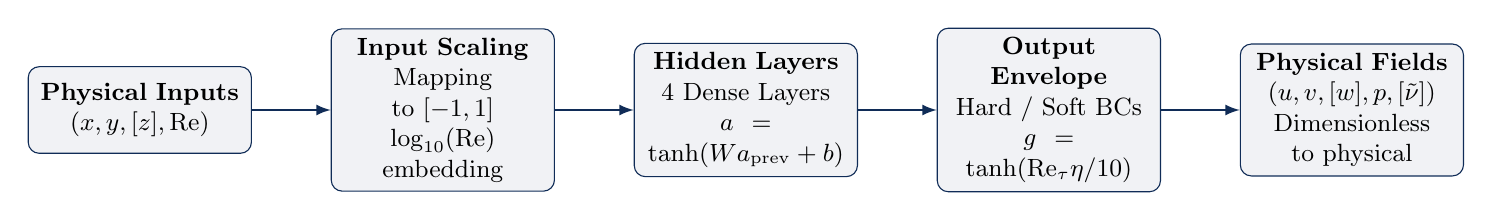
\begin{tikzpicture}[node distance=1.0cm, auto,
    block/.style={rectangle, draw=primary, fill=primary!6, text width=2.6cm, text centered, rounded corners, minimum height=1.1cm, font=\small},
    line/.style={draw=primary, -latex, thick}]
    
    \node [block] (input) {\textbf{Physical Inputs}\\$(x, y, [z], \mathrm{Re})$};
    \node [block, right=1.0cm of input] (scale) {\textbf{Input Scaling}\\Mapping to $[-1, 1]$\\$\log_{10}(\mathrm{Re})$ embedding};
    \node [block, right=1.0cm of scale] (hidden) {\textbf{Hidden Layers}\\4 Dense Layers\\$a = \tanh(W a_{\mathrm{prev}} + b)$};
    \node [block, right=1.0cm of hidden] (env) {\textbf{Output Envelope}\\Hard / Soft BCs\\$g = \tanh(\mathrm{Re}_\tau \eta / 10)$};
    \node [block, right=1.0cm of env] (phys) {\textbf{Physical Fields}\\$(u, v, [w], p, [\tilde{\nu}])$\\Dimensionless to physical};
    
    \path [line] (input) -- (scale);
    \path [line] (scale) -- (hidden);
    \path [line] (hidden) -- (env);
    \path [line] (env) -- (phys);
\end{tikzpicture}%
}
\caption{Forward pass architecture of the Physics-Informed Neural Network. Inputs are scaled to $[-1, 1]$ before passing through 4 hidden layers of width 80 (Stages 1--3) or 64 (Stages 4--5) with $\tanh$ activations. Outputs are converted to physical velocity, pressure, and eddy viscosity fields through hard boundary envelopes in turbulent stages or soft penalty formulations in laminar stages.}
\label{fig:forward_pass_flowchart}
\end{figure}

\begin{figure}[H]
\centering
\hyphenpenalty=10000
\exhyphenpenalty=10000
\resizebox{\linewidth}{!}{%
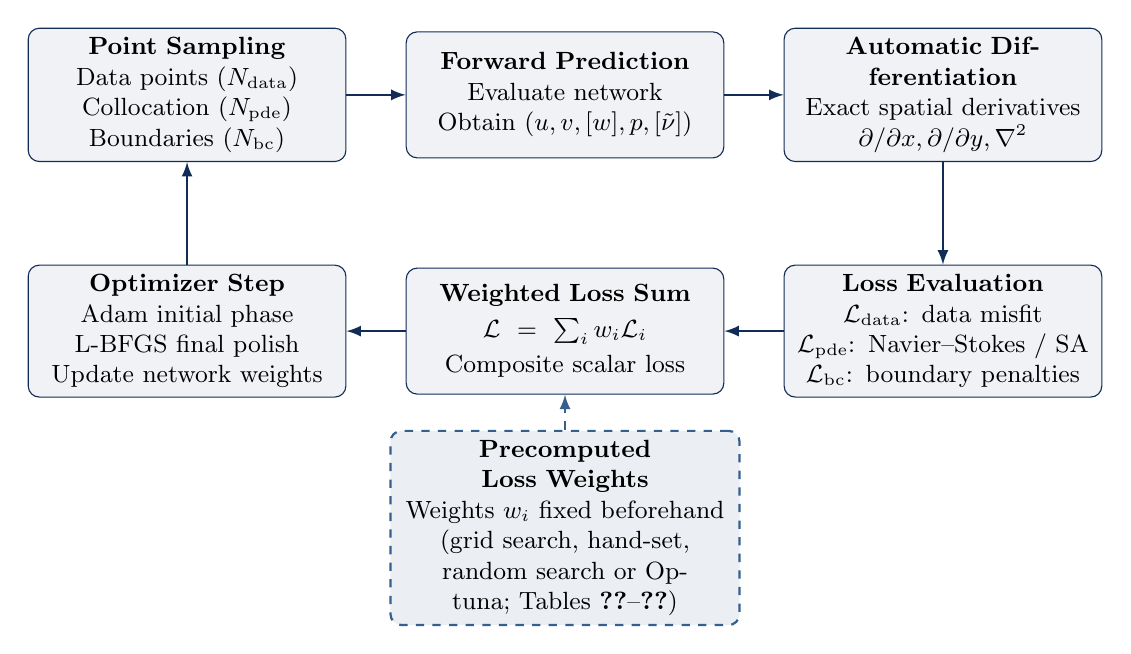
\begin{tikzpicture}[
        block/.style={rectangle, draw=primary, fill=primary!6, text width=3.8cm, text centered, rounded corners, minimum height=1.6cm, font=\small},
    prebox/.style={rectangle, draw=secondary, fill=secondary!10, text width=4.2cm, text centered, rounded corners, minimum height=1.6cm, font=\small, dashed, thick},
    line/.style={draw=primary, -latex, thick},
    dashline/.style={draw=secondary, -latex, thick, dashed}]
    
    % The iterative loop nodes
    \node [block] (sample) at (0, 0) {\textbf{Point Sampling}\\Data points ($N_{\mathrm{data}}$)\\Collocation ($N_{\mathrm{pde}}$)\\Boundaries ($N_{\mathrm{bc}}$)};
    \node [block] (pred) at (4.8, 0) {\textbf{Forward Prediction}\\Evaluate network\\Obtain $(u, v, [w], p, [\tilde{\nu}])$};
    \node [block] (autograd) at (9.6, 0) {\textbf{Automatic Differentiation}\\Exact spatial derivatives\\$\partial / \partial x, \partial / \partial y, \nabla^2$};
    \node [block] (losses) at (9.6, -3.0) {\textbf{Loss Evaluation}\\$\mathcal{L}_{\mathrm{data}}$: data misfit\\$\mathcal{L}_{\mathrm{pde}}$: Navier--Stokes / SA\\$\mathcal{L}_{\mathrm{bc}}$: boundary penalties};
    \node [block] (weighted) at (4.8, -3.0) {\textbf{Weighted Loss Sum}\\\vspace{0.2em}$\mathcal{L} = \sum_i w_i \mathcal{L}_i$\\\vspace{0.2em}Composite scalar loss};
    \node [block] (opt) at (0, -3.0) {\textbf{Optimizer Step}\\Adam initial phase\\L-BFGS final polish\\Update network weights};
    
    % Precomputed weights box outside the loop
    \node [prebox] (weights) at (4.8, -5.5) {\textbf{Precomputed Loss Weights}\\Weights $w_i$ fixed beforehand\\(grid search, hand-set, random search or Optuna; Tables~\ref{tab:training_recipes_laminar}--\ref{tab:training_recipes_turb})};
    
    % Loop connections
    \path [line] (sample) -- (pred);
    \path [line] (pred) -- (autograd);
    \path [line] (autograd) -- (losses);
    \path [line] (losses) -- (weighted);
    \path [line] (weighted) -- (opt);
    \path [line] (opt) -- (sample);
    
    % Connection from precomputed weights into weighted sum
    \path [dashline] (weights) -- (weighted);
\end{tikzpicture}%
}
\caption{Training and optimization procedure of the PINN pipeline. Collocation, reference data, and boundary points are sampled across operating Reynolds numbers. Automatic differentiation evaluates governing PDE residuals without a numerical grid. Individual loss terms are balanced via composite weights determined beforehand (Tables~\ref{tab:training_recipes_laminar}--\ref{tab:training_recipes_turb}), followed by sequential Adam and L-BFGS optimization.}
\label{fig:training_flowchart}
\end{figure}






\subsection{Reynolds-Number Splits}
\label{sec:reynolds_splits}
Table~\ref{tab:reynolds_splits} reports the exact Reynolds-number assignments across training, validation, and test partitions for all five stages, along with the characteristic length and velocity scales defining $\mathrm{Re}$. The validation Reynolds number $\mathrm{Re}=88{,}000$ in Stages 4 and 5 lies above the highest training Reynolds number ($80{,}000$).

\begin{table}[H]
\centering
\small
\resizebox{\textwidth}{!}{%
\begin{tabular}{lcccccc}
\toprule
\textbf{Stage} & \textbf{Training $\mathrm{Re}$} & \textbf{Validation $\mathrm{Re}$} & \textbf{Test $\mathrm{Re}$ (Interp)} & \textbf{Test $\mathrm{Re}$ (Extrap)} & \textbf{Length Scale} & \textbf{Velocity Scale} \\
\midrule
1. Laminar Channel & 50, 100, 200, 500 & none & 300 & 600 & $D_h = 4h = 0.20\,\text{m}$ & $U_0$ (mean inlet) \\
2. Laminar Pipe & 50, 100, 200, 500 & none & 300 & 600 & $D = 2R = 0.10\,\text{m}$ & $U_0$ (mean inlet) \\
3. Laminar Duct & 50, 100, 200, 500 & none & 300 & 600 & $D_h = 4A/P = 0.1333\,\text{m}$ & $U_b$ (bulk velocity) \\
4. Turbulent Channel & 10k, 20k, 40k, 80k & 14k, 56k, 88k & 28k & 96k (1.2$\times$), 120k (1.5$\times$) & $D_h = 4h = 0.20\,\text{m}$ & $U_b$ (bulk velocity) \\
5. Turbulent Pipe & 10k, 20k, 40k, 80k & 14k, 56k, 88k & 28k & 96k (1.2$\times$), 120k (1.5$\times$) & $D = 2R = 0.10\,\text{m}$ & $U_b$ (bulk velocity) \\
\bottomrule
\end{tabular}%
}
\caption{Reynolds-number operating partitions and definition scales across Stages 1--5. For Stage~3, $\mathrm{Re}=600$ is at the edge of the normalized range (Sec.~\ref{sec:stage3_arch}). In Stages 4 and 5, $\mathrm{Re}=88{,}000$ (validation) lies above the maximum training value ($80{,}000$).}
\label{tab:reynolds_splits}
\end{table}


\subsection{Error Metrics}
\label{sec:error_metrics}
Model performance is evaluated using standardized statistical metrics:
\begin{itemize}[leftmargin=1.5em]
    \item \textbf{Relative $L_2$ Error ($E_f$):} Defined for any predicted field $f$ over all evaluation points of the reference grid as
    \begin{equation}
    E_f = \frac{\|f_{\mathrm{PINN}} - f_{\mathrm{ref}}\|_2}{\|f_{\mathrm{ref}}\|_2} = \frac{\sqrt{\sum_{i=1}^N (f_{\mathrm{PINN},i} - f_{\mathrm{ref},i})^2}}{\sqrt{\sum_{i=1}^N f_{\mathrm{ref},i}^2}}.
    \end{equation}
    For velocity fields in turbulent stages, normalization uses bulk velocity $U_b$ (or $0.05 u_\tau$ for wall-normal velocity $V$) to avoid division by zero near walls.
    \item \textbf{Pointwise Error Maps and Percentiles:} Local absolute errors $|f_{\mathrm{PINN}} - f_{\mathrm{ref}}|$ are evaluated across the full spatial mesh. Summary percentiles (median, P95, P99) characterize the distribution and peak local discrepancies.
    \item \textbf{Skin Friction Coefficient Error ($C_f$):} Evaluated as the relative $L_2$ error of the wall shear stress coefficient $C_f(x) = 2\tau_w(x) / (\rho U_b^2)$ with respect to the reference solver.
    \item \textbf{Interpolation vs.\ Extrapolation Testing:} Test Reynolds numbers are categorized into interpolation (within the training span $[\mathrm{Re}_{\min}, \mathrm{Re}_{\max}]$) and extrapolation (1.2 and 1.5 times the largest training Reynolds number, 80,000; for Stage~3, $\mathrm{Re}=600$ lies at the edge of the normalized range, Sec.~\ref{sec:stage3_arch}).
    \item \textbf{Kinematic and Gauge Pressure:} In laminar stages, kinematic pressure $p/\rho$ [m$^2$/s$^2$] is reported relative to zero outlet gauge pressure. In turbulent stages, normalized pressure $P/(\rho U_b^2)$ is reported.
    \item \textbf{Generalization Ratio:} Defined as the ratio of test-set relative error to training-set relative error, measuring the degree of overfitting.
\end{itemize}


\section{Stage 1: Developing 2D Laminar Channel Flow}
\label{sec:stage1}

\subsection{Geometry and Physical Problem Setup}
Stage 1 models the developing laminar entrance flow of an incompressible Newtonian fluid between two parallel flat plates. The computational domain is rectangular: $x \in [0, L]$ with $L = 4.0\,\text{m}$, and $y \in [-h, h]$ with channel half-height $h = 0.05\,\text{m}$ (full channel height $2h = 0.10\,\text{m}$). The hydraulic diameter for infinite parallel plates is $D_h = 4A/P = 4(2h)/2 = 4h = 0.20\,\text{m}$. Fluid kinematic viscosity is $\nu = 1.0\times 10^{-4}\,\text{m}^2/\text{s}$.

\begin{figure}[H]
\centering
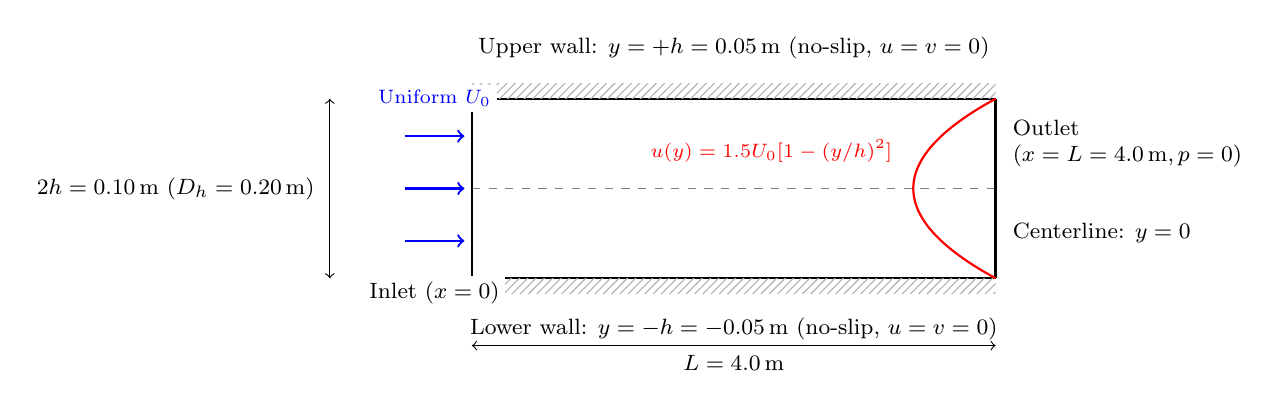
\begin{tikzpicture}[scale=0.95]
    \node[above, font=\footnotesize] at (3.5, 1.6) {Upper wall: $y = +h = 0.05\,\text{m}$ (no-slip, $u=v=0$)};
    \draw[thick] (0, 1.2) -- (7.0, 1.2);
    \fill[pattern=north east lines, pattern color=gray!60] (0, 1.2) rectangle (7.0, 1.4);
    \draw[thick] (0, -1.2) -- (7.0, -1.2);
    \fill[pattern=north east lines, pattern color=gray!60] (0, -1.4) rectangle (7.0, -1.2);
    \node[below, font=\footnotesize] at (3.5, -1.6) {Lower wall: $y = -h = -0.05\,\text{m}$ (no-slip, $u=v=0$)};
    \draw[dashed, gray] (0, 0) -- (7.0, 0);
    \draw[thick] (0, -1.2) -- (0, 1.2);
    \draw[blue, thick, ->] (-0.9, 0.7) -- (-0.1, 0.7);
    \draw[blue, thick, ->] (-0.9, 0.0) -- (-0.1, 0.0);
    \draw[blue, thick, ->] (-0.9, -0.7) -- (-0.1, -0.7);
    \node[blue, font=\scriptsize, above=3mm, fill=white, inner sep=2pt] at (-0.5, 0.7) {Uniform $U_0$};
    \node[font=\footnotesize, below=3mm, fill=white, inner sep=2pt] at (-0.5, -0.85) {Inlet ($x=0$)};
    \draw[thick] (7.0, -1.2) -- (7.0, 1.2);
    \node[right, font=\footnotesize, align=left] at (7.1, 0.6) {Outlet\\($x = L = 4.0\,\text{m}, p = 0$)};
    \node[right, font=\footnotesize] at (7.1, -0.6) {Centerline: $y = 0$};
    \draw[domain=-1.2:1.2, smooth, variable=\y, red, thick] plot ({7.0 - 1.1*(1 - (\y/1.2)*(\y/1.2))}, {\y});
    \node[red, font=\scriptsize, fill=white, inner sep=2pt, left] at (5.7, 0.5) {$u(y) = 1.5 U_0 [1 - (y/h)^2]$};
    \draw[<->] (0, -2.1) -- (7.0, -2.1) node[midway, below, font=\footnotesize] {$L = 4.0\,\text{m}$};
    \draw[<->] (-1.9, -1.2) -- (-1.9, 1.2) node[midway, left=2pt, font=\footnotesize] {$2h = 0.10\,\text{m}$ ($D_h = 0.20\,\text{m}$)};
\end{tikzpicture}
\caption{Stage 1 geometry: laminar channel entrance development between parallel plates.}
\label{fig:stage1_geom}
\end{figure}

The Reynolds number is defined based on the hydraulic diameter:
\begin{equation}
\mathrm{Re} = \frac{U_0 D_h}{\nu} = \frac{U_0 \cdot 0.20}{1.0\times 10^{-4}} = 2000\,U_0 \implies U_0(\mathrm{Re}) = 0.0005\,\mathrm{Re}\,\text{m/s}.
\end{equation}
At $\mathrm{Re}=100$, bulk velocity is $U_0 = 0.05\,\text{m/s}$, and dynamic pressure scale is $p_{\mathrm{scale}} = 0.5 U_0^2 = 0.00125\,\text{m}^2/\text{s}^2$. The training set covers $\mathrm{Re} \in \{50, 100, 200, 500\}$; $\mathrm{Re}=300$ tests interpolation, and $\mathrm{Re}=600$ tests extrapolation.
% src: 1/model.py:54

\subsection{Governing Equations and Dimensionless Formulation}
The flow is governed by the two-dimensional steady incompressible Navier--Stokes equations in Cartesian coordinates:
\begin{align}
\frac{\partial u}{\partial x} + \frac{\partial v}{\partial y} &= 0, \\
u \frac{\partial u}{\partial x} + v \frac{\partial u}{\partial y} &= -\frac{\partial p}{\partial x} + \nu \left(\frac{\partial^2 u}{\partial x^2} + \frac{\partial^2 u}{\partial y^2}\right), \\
u \frac{\partial v}{\partial x} + v \frac{\partial v}{\partial y} &= -\frac{\partial p}{\partial y} + \nu \left(\frac{\partial^2 v}{\partial x^2} + \frac{\partial^2 v}{\partial y^2}\right),
\end{align}
where $p = P/\rho$ denotes kinematic pressure ($\text{m}^2/\text{s}^2$). Boundary conditions are:
\begin{itemize}[leftmargin=1.5em]
    \item Inlet ($x=0$): Uniform velocity $u(0, y) = U_0(\mathrm{Re}), v(0, y) = 0$.
    \item Walls ($y = \pm h$): No-slip condition $u(x, \pm h) = 0, v(x, \pm h) = 0$.
    \item Outlet ($x=L$): Gauge pressure reference $p(L, y) = 0, \partial u/\partial x = 0, \partial v/\partial x = 0$.
\end{itemize}
% src: 1/config.py:48; atkinson1969; shah1978
Hydrodynamic entrance length $L_e$ characterizes the axial development distance, benchmarked against the empirical correlation of Durst et al.~\cite[Eq.~(2b), p.~8]{ray2017}:
\begin{equation}
\frac{L_e}{D_h} = \left[(0.3155)^{1.6} + (0.01105\,\mathrm{Re})^{1.6}\right]^{1/1.6}.
\end{equation}
For $D_h = 0.20\,\text{m}$, the correlation gives $L_e = 0.239\,\text{m}$ at $\mathrm{Re}=100$, $0.673\,\text{m}$ at $\mathrm{Re}=300$, and $1.332\,\text{m}$ at $\mathrm{Re}=600$. All entrance lengths fit within the computational domain length $L = 4.0\,\text{m}$.

\subsection{Reference Solver and Training Data Generation}
Reference data was generated using an independent Python solver implementing an implicit marching finite-difference method of Hornbeck type~\cite[Ch.~6, pp.~153--160]{hornbeck1973} (\texttt{1/entrance\_solver.py}).
The reference solver assumes the parabolized boundary-layer equations:
\begin{align}
u \frac{\partial u}{\partial x} + v \frac{\partial u}{\partial y} &= -\frac{1}{\rho}\frac{dP}{dx} + \nu \frac{\partial^2 u}{\partial y^2}, \\
\frac{\partial u}{\partial x} + \frac{\partial v}{\partial y} &= 0.
\end{align}
The solver drops streamwise viscous diffusion ($\partial^2 u/\partial x^2 = 0$) and drops the transverse momentum equation entirely ($\partial p/\partial y = 0 \implies p = p(x)$). It discretizes the domain onto a grid of $n_x = 500$ axial stations and $n_y = 81$ transverse nodes ($500 \times 81$). At each station, it solves a tridiagonal linear system for $u$ and superposes particular and homogeneous solutions to satisfy global mass conservation $\int_{-h}^h u\,dy = 2h U_0$. 

As noted in Section~\ref{sec:elliptic_vs_parabolic}, the network is trained on the full Navier--Stokes equations whereas the reference solver neglects axial diffusion and the cross-stream pressure gradient; the resulting difference is largest near the inlet.

\subsection{Network Design and Hyperparameters}
The Stage 1 neural network (\texttt{1/model.py}, class \texttt{ChannelPINN}) is a fully connected Multilayer Perceptron. It takes three normalized inputs:
\begin{equation}
\hat{x} = \frac{x}{L} \in [0, 1], \quad \hat{y} = \frac{y}{h} \in [-1, 1], \quad \mathrm{Re}_n = 2\frac{\log_{10}(\mathrm{Re}/50)}{\log_{10}(500/50)} - 1 \in [-1, 1].
\end{equation}
The architecture comprises four hidden layers of 80 neurons with $\tanh$ activations (layer dimensions $[3, 80, 80, 80, 80, 3]$). Trainable weights and biases total:
\begin{equation}
% src: 1/outputs/channel_pinn_hybrid.pt
N_{\mathrm{params}} = (3\times 80 + 80) + 3\times (80\times 80 + 80) + (80\times 3 + 3) = 320 + 3\times 6480 + 243 = \mathbf{20{,}003}.
\end{equation}
Weights are initialized using Xavier normal initialization~\cite[Eq.~(12), p.~253]{glorot2010}. The training protocol uses Adam optimization for 3000 iterations with an initial learning rate of $8.0\times 10^{-4}$ decayed via \texttt{StepLR} ($\gamma=0.7$ every 400 steps), followed by an L-BFGS polish for 200 iterations (strong-Wolfe line search). At each training iteration, $N_{\mathrm{data}} = 200$ reference-solution data points are drawn at random from the reference grid, and $N_{\mathrm{pde}} = 1{,}500$ collocation points are drawn anew with power-law clustering near the inlet ($x$). Collocation point counts per iteration are: 200 reference data points, 1,500 interior PDE points, and 150 boundary points.

\subsection{Composite Loss Formulation and Final Weights}
The composite loss function minimized during training is:
\begin{equation}
\mathcal{L} = w_{\mathrm{data}}\mathcal{L}_{\mathrm{data}} + w_{\mathrm{pde}}\mathcal{L}_{\mathrm{pde}} + w_{\mathrm{inlet}}\mathcal{L}_{\mathrm{inlet}} + w_{\mathrm{wall}}\mathcal{L}_{\mathrm{wall}} + w_{\mathrm{outlet}}\mathcal{L}_{\mathrm{outlet}}.
\end{equation}
The loss terms are defined as:
\begin{align}
\mathcal{L}_{\mathrm{data}} &= \frac{1}{N_d} \sum_{i=1}^{N_d} \left[ \left(\frac{u_i - u_i^{\mathrm{ref}}}{U_0}\right)^2 + \left(\frac{v_i - v_i^{\mathrm{ref}}}{U_0}\right)^2 + \left(\frac{p_i - p_i^{\mathrm{ref}}}{p_{\mathrm{scale}}}\right)^2 \right], \\
\mathcal{L}_{\mathrm{pde}} &= \frac{1}{N_c} \sum_{j=1}^{N_c} \left[ \mathcal{R}_{\mathrm{cont}}^2 + \mathcal{R}_{\mathrm{mom},x}^2 + \mathcal{R}_{\mathrm{mom},y}^2 \right], \\
\mathcal{L}_{\mathrm{inlet}} &= \frac{1}{N_{\mathrm{in}}} \sum_{k=1}^{N_{\mathrm{in}}} \left[ \left(\frac{u(0, y_k) - U_0}{U_0}\right)^2 + \left(\frac{v(0, y_k)}{U_0}\right)^2 \right], \\
\mathcal{L}_{\mathrm{wall}} &= \frac{1}{N_w} \sum_{k=1}^{N_w} \left[ \left(\frac{u(x_k, \pm h)}{U_0}\right)^2 + \left(\frac{v(x_k, \pm h)}{U_0}\right)^2 \right], \\
\mathcal{L}_{\mathrm{outlet}} &= \frac{1}{N_{\mathrm{out}}} \sum_{k=1}^{N_{\mathrm{out}}} \left(\frac{p(L, y_k)}{p_{\mathrm{scale}}}\right)^2.
\end{align}
The final fixed weights read from \texttt{1/train\_hybrid.py} are:
\begin{equation}
% src: 1/train_hybrid.py Line 45
w_{\mathrm{data}} = 20.0, \quad w_{\mathrm{pde}} = 1.0, \quad w_{\mathrm{inlet}} = 5.0, \quad w_{\mathrm{wall}} = 5.0, \quad w_{\mathrm{outlet}} = 1.0.
\end{equation}
The relative physics-to-data loss weight ratio is $w_{\mathrm{pde}} / w_{\mathrm{data}} = 1.0 / 20.0 = \mathbf{0.05}$.

\subsection{Forward Pass at a Single Point}
The pre-activation vector $z = W a_{\mathrm{prev}} + b$ represents the affine combination entering each layer, while the post-activation $a = \tanh(z)$ is its bounded output. Matrix $\|W\|_F$ denotes the Frobenius norm of the layer weight matrix, $\|b\|_2$ is the Euclidean norm of the bias vector, and $z[1:4]$ reports the numerical values of the first four neurons of each layer.

To establish exact numerical reproducibility, Table~\ref{tab:stage1_act} presents layer activations evaluated directly from checkpoint \texttt{1/outputs/channel\_pinn\_hybrid.pt} at $(x=0.5\,\text{m}, y=0.02\,\text{m}, \mathrm{Re}=100)$.
\begin{table}[H]
\centering
\resizebox{\linewidth}{!}{%
\begin{tabular}{lcccc}
\toprule
\textbf{Network Layer} & \textbf{Pre-activations} $z_{[1:4]}$ & \textbf{Post-activations} $a_{[1:4]} = \tanh(z)$ & $\|W\|_F$ & $\|b\|_2$ \\
\midrule
Hidden 1 & $[-0.0579, 0.1571, -0.0009, -0.1015]$ & $[-0.0579, 0.1558, -0.0009, -0.1011]$ & 3.43 & 0.96 \\
Hidden 2 & $[-0.7194, 0.7283, 0.0744, -0.5888]$ & $[-0.6166, 0.6220, 0.0742, -0.5290]$ & 11.30 & 0.70 \\
Hidden 3 & $[-1.4141, -2.8177, 0.9572, 2.0372]$ & $[-0.8884, -0.9929, 0.7430, 0.9666]$ & 12.00 & 0.51 \\
Hidden 4 & $[1.2799, -1.5198, 3.7344, 0.2901]$ & $[0.8565, -0.9087, 0.9989, 0.2822]$ & 12.12 & 0.40 \\
Output & $[1.2933, 0.0168, 16.6964]$ & N/A & 5.44 & 0.29 \\
\bottomrule
\end{tabular}%
}
\caption{Deterministic layer-by-layer forward pass evaluated at $(x=0.5\,\text{m}, y=0.02\,\text{m}, \mathrm{Re}=100)$. Normalized input vector: $[0.1250, 0.4000, -0.3979]^{\mathsf T}$. Checkpoint SHA256: \texttt{4d200a420951a10b...}.}
\label{tab:stage1_act}
\end{table}
Normalized coordinates evaluate to $\hat{x} = 0.125$, $\hat{y} = 0.400$, and $\mathrm{Re}_n = -0.3979$. The network outputs normalized vector $\hat{\mathbf{u}} = [1.2933, 0.0168, 16.6964]^T$.
Rescaling by $U_0 = 0.05\,\text{m/s}$ and dynamic pressure scale $p_{\mathrm{scale}} = 0.5 U_0^2 = 0.00125\,\text{m}^2/\text{s}^2$ yields:
\begin{align}
% src: provenance.json stage1 physical_predictions
u &= 1.2933 \times 0.05 = \mathbf{0.06466\,\text{m/s}} \quad (\text{reference: } 0.06301\,\text{m/s}, \text{ error } 2.62\%), \\
v &= 0.0168 \times 0.05 = \mathbf{0.00084\,\text{m/s}} \quad (\text{reference: } 0.00078\,\text{m/s}, \text{ error } 7.69\%), \\
p &= 16.6964 \times 0.00125 = \mathbf{0.02087\,\text{m}^2/\text{s}^2} \quad (\text{reference gauge: } 0.02100\,\text{m}^2/\text{s}^2, \text{ error } 0.64\%).
\end{align}

\subsection{Empirical Results and Performance Evaluation}
Table~\ref{tab:stage1_metrics} compiles the full-domain relative $L_2$ errors across all six evaluated Reynolds numbers.
\begin{table}[H]
\centering
\resizebox{\textwidth}{!}{
\begin{tabular}{lcccccc}
\toprule
\textbf{Metric Variable} & $\mathbf{Re=50}$ & $\mathbf{Re=100}$ & $\mathbf{Re=200}$ & $\mathbf{Re=300}$ (TEST-interp) & $\mathbf{Re=500}$ & $\mathbf{Re=600}$ (TEST-extrap) \\
\midrule
$u$ (Axial Velocity Rel $L_2$) & 5.00\% & 5.69\% & 4.10\% & 4.46\% & 3.88\% & 4.25\% \\
$v$ (Vertical Velocity Rel $L_2$) & 2.91\% & 2.15\% & 1.27\% & 1.34\% & 1.11\% & 1.14\% \\
$p$ (Kinematic Pressure Rel $L_2$) & 6.30\% & 6.21\% & 4.95\% & 8.35\% & 6.12\% & 6.72\% \\
\bottomrule
\end{tabular}
}
\caption{Stage 1: Full-domain relative $L_2$ errors across training and test Reynolds numbers (Source: \texttt{1/outputs/metrics\_full\_domain.csv}).}
\label{tab:stage1_metrics}
\end{table}


\begin{figure}[H]
\centering
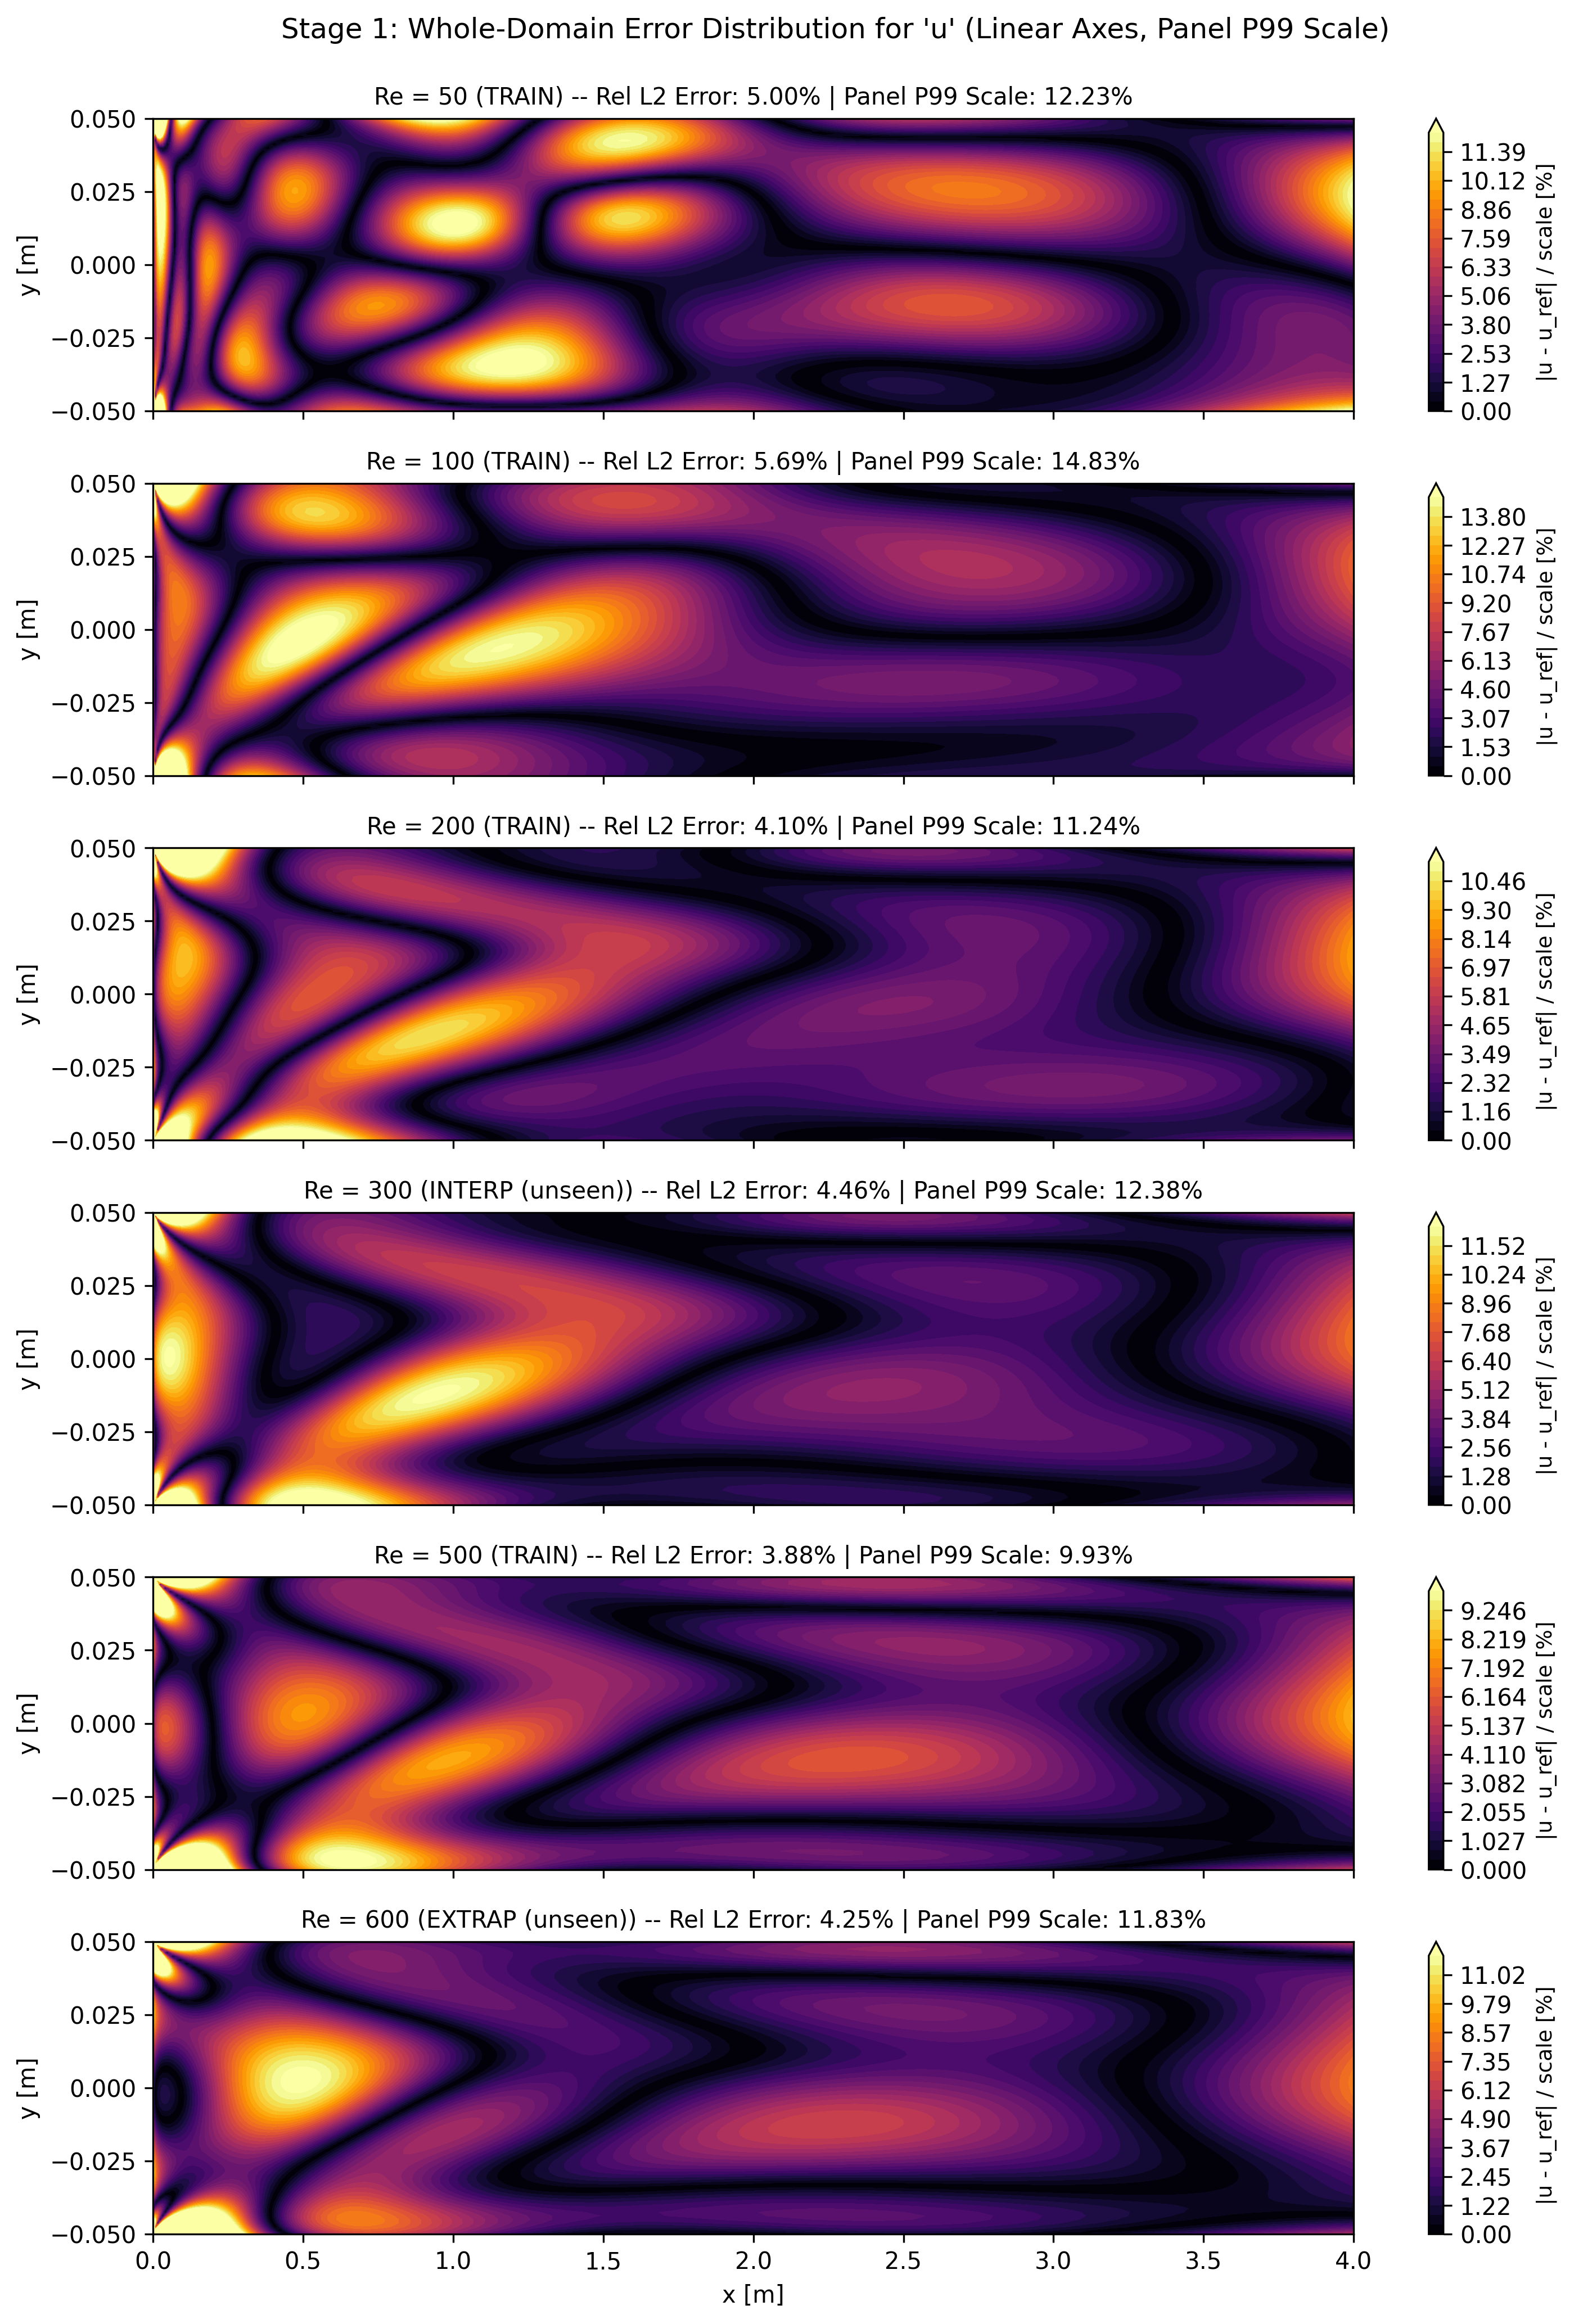
\includegraphics[width=0.95\textwidth]{stage1_error_u.png}
\caption{Stage 1: Linear-axis axial velocity error $|u - u_{\mathrm{ref}}|/U_0$ [\%] across the Reynolds sweep.}
\label{fig:stage1_errors}
\end{figure}

\begin{figure}[H]
\centering
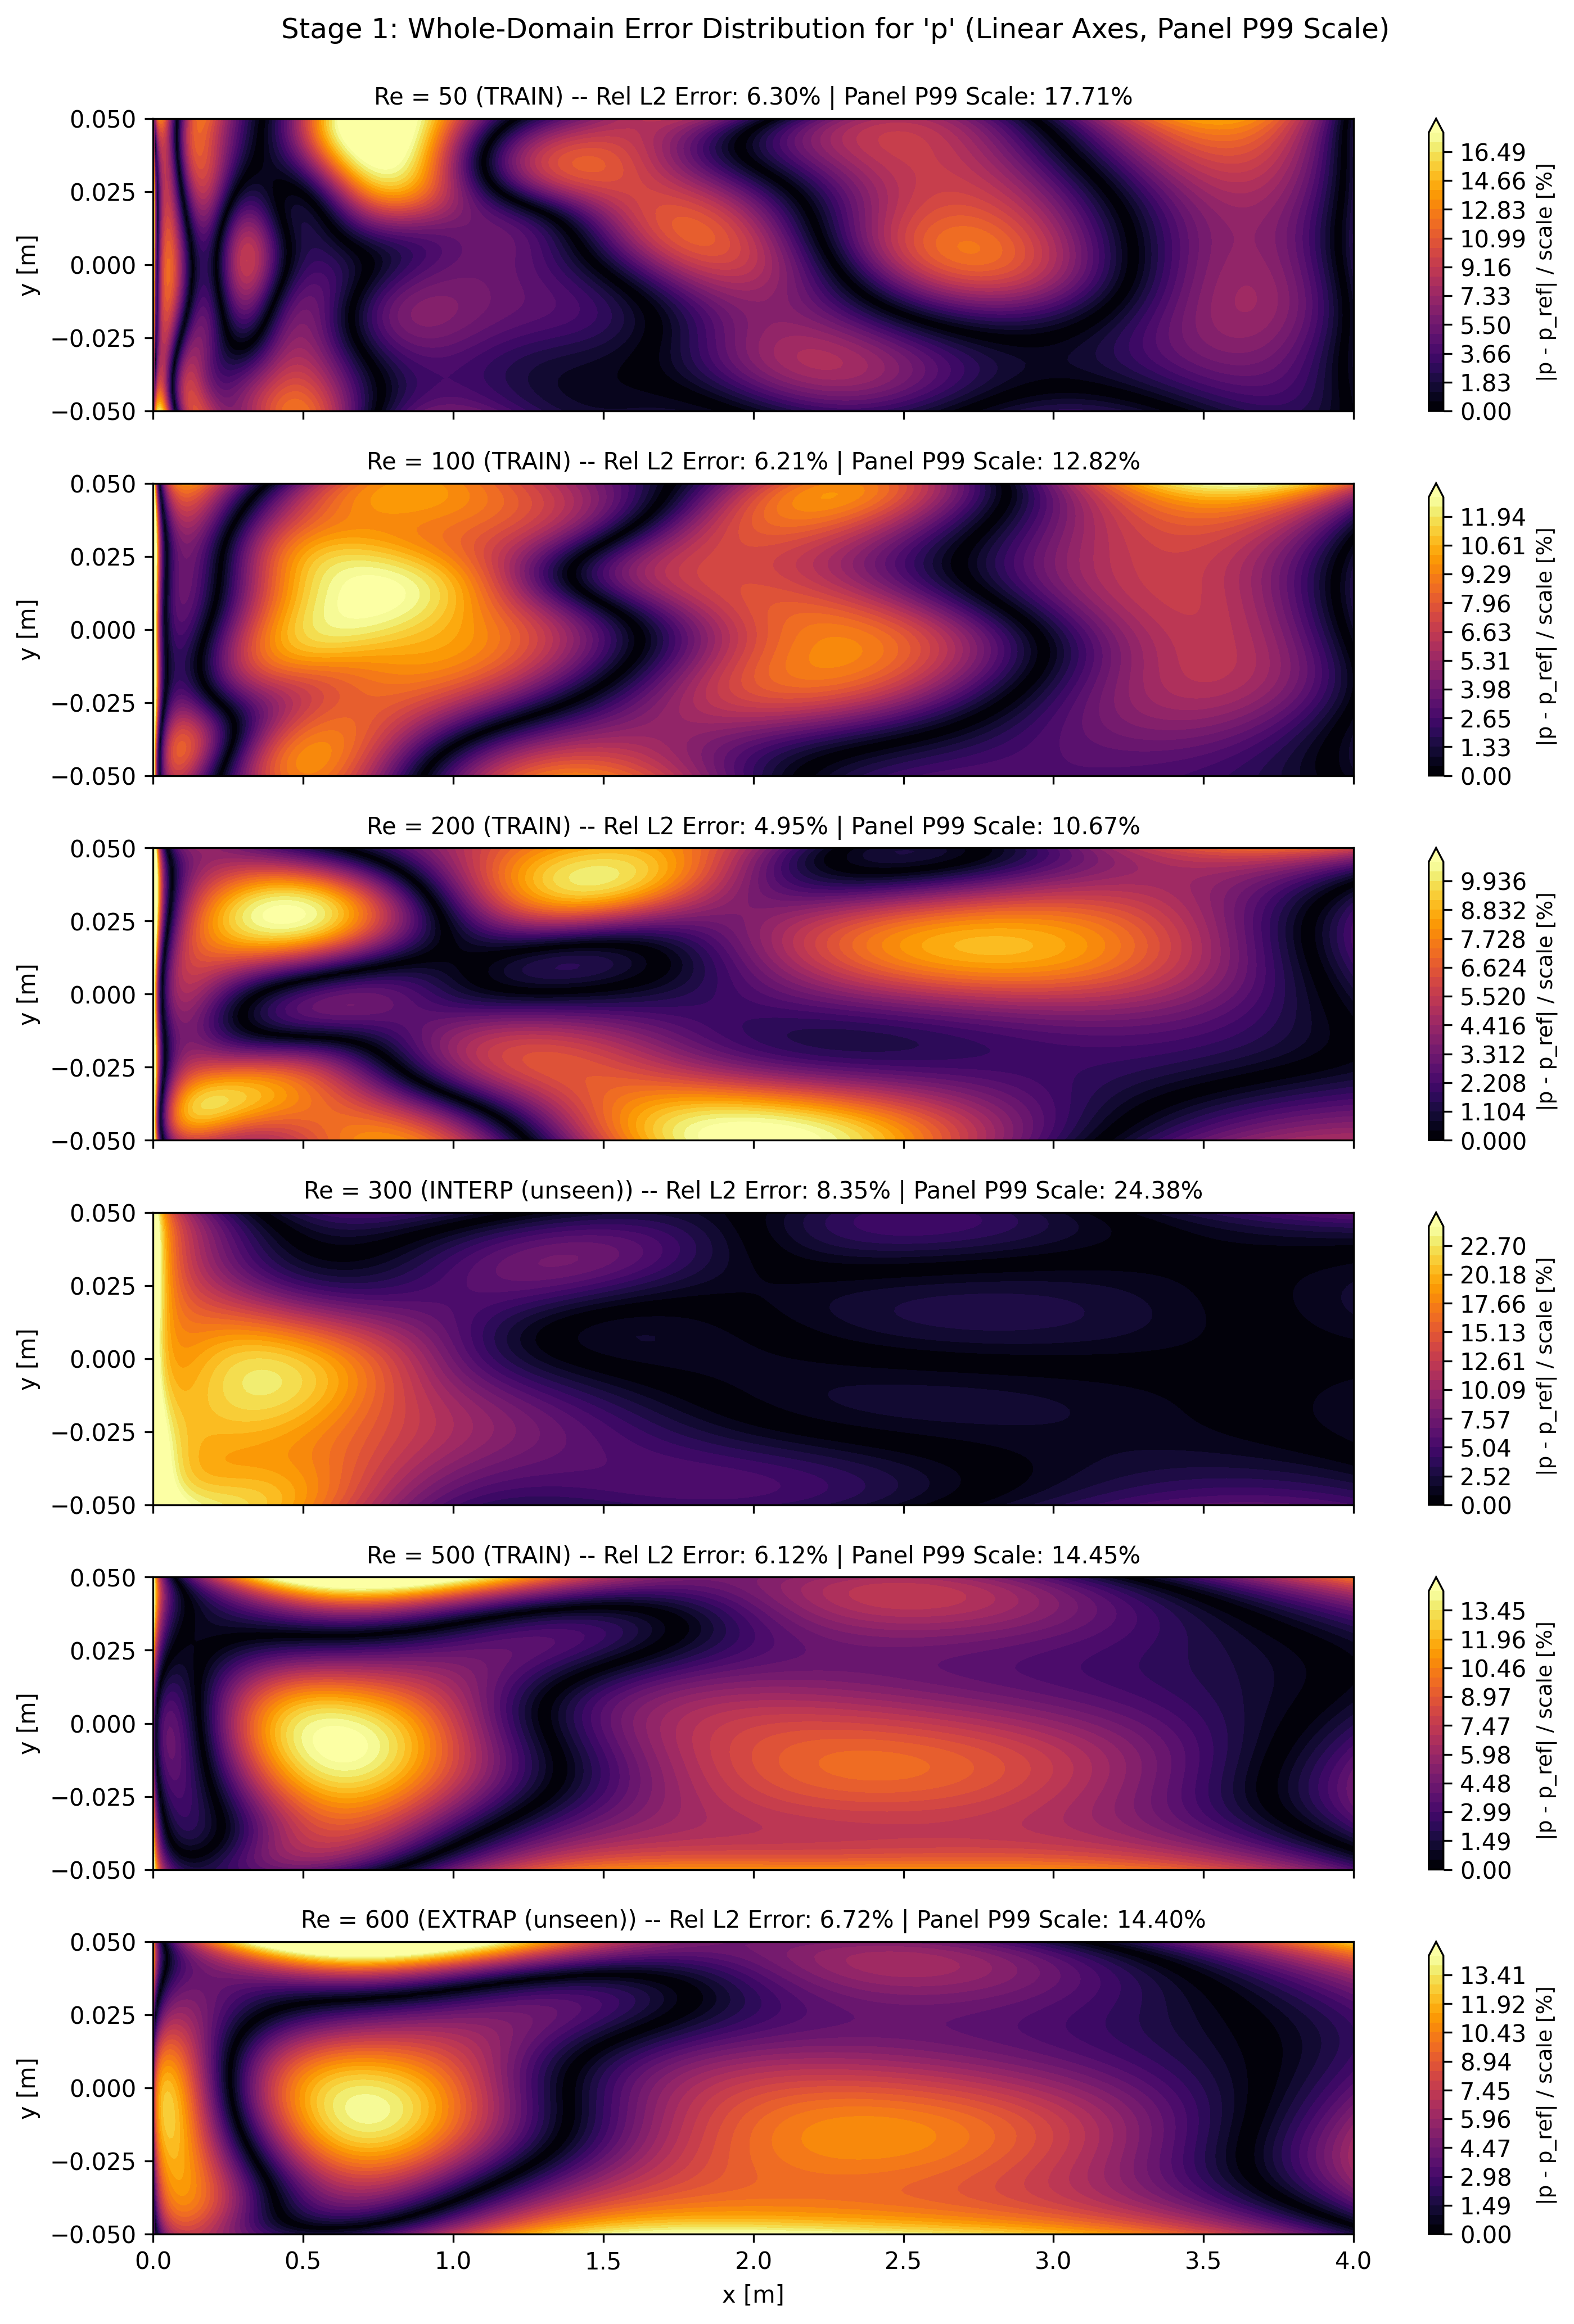
\includegraphics[width=0.95\textwidth]{stage1_error_p.png}
\caption{Stage 1: Kinematic pressure error $|p - p_{\mathrm{ref}}|/p_{\mathrm{scale}}$ [\%] across the Reynolds sweep.}
\label{fig:stage1_error_p}
\end{figure}

\noindent\textbf{Interpretation of Results and Error Maps:}
% % src: 1/outputs/metrics_full_domain.csv
% src: 1/outputs/metrics_full_domain.csv; 1/outputs/reference_data.npz
Across all test cases, global relative $L_2$ errors for streamwise velocity $u$ remain between $3.88\%$ and $5.69\%$. As shown in Figure~\ref{fig:stage1_errors}, the local pointwise errors exhibit median values between $2.42\%$ and $3.48\%$ with 95th percentiles (P95) between $6.82\%$ and $11.88\%$ (P99 reaching $9.93\%$--$14.83\%$). Error distributions show that peak errors do not remain confined to the inlet region ($x < 0.5\,\text{m}$); distinct error lobes persist along the shear layers downstream towards the channel exit. Transverse velocity $v$ achieves global errors of $1.11\%$--$2.91\%$, while pressure errors range between $4.95\%$ and $8.35\%$.


\subsection{Predicted Flow Fields}
Figures~\ref{fig:stage1_pred_re100} and~\ref{fig:stage1_pred_re600} present the continuous flow-field predictions generated by the trained Stage~1 PINN across the planar conduit ($L=4.0\,\text{m}$, $h=0.05\,\text{m}$, total gap $2h=0.10\,\text{m}$) at Reynolds numbers $\mathrm{Re} = 100$ and $600$. Because the channel domain is elongated ($L/(2h) = 40$), the wall-normal axis is stretched by a factor $k \approx 14$ for visual clarity.

The predicted flow fields depict the hydrodynamic development from a uniform inlet velocity ($u = U_0$, $v = 0$) into the parabolic Poiseuille profile far downstream. Transverse velocity $v$ is non-zero exclusively in the near-inlet boundary-layer growth region, directing mass towards the channel center, before decaying to zero as the flow approaches the fully developed state. Kinematic pressure falls monotonically along the conduit, providing the driving force balancing viscous wall shear.

\begin{figure}[H]
\centering
\begin{subfigure}[b]{0.48\textwidth}
\centering
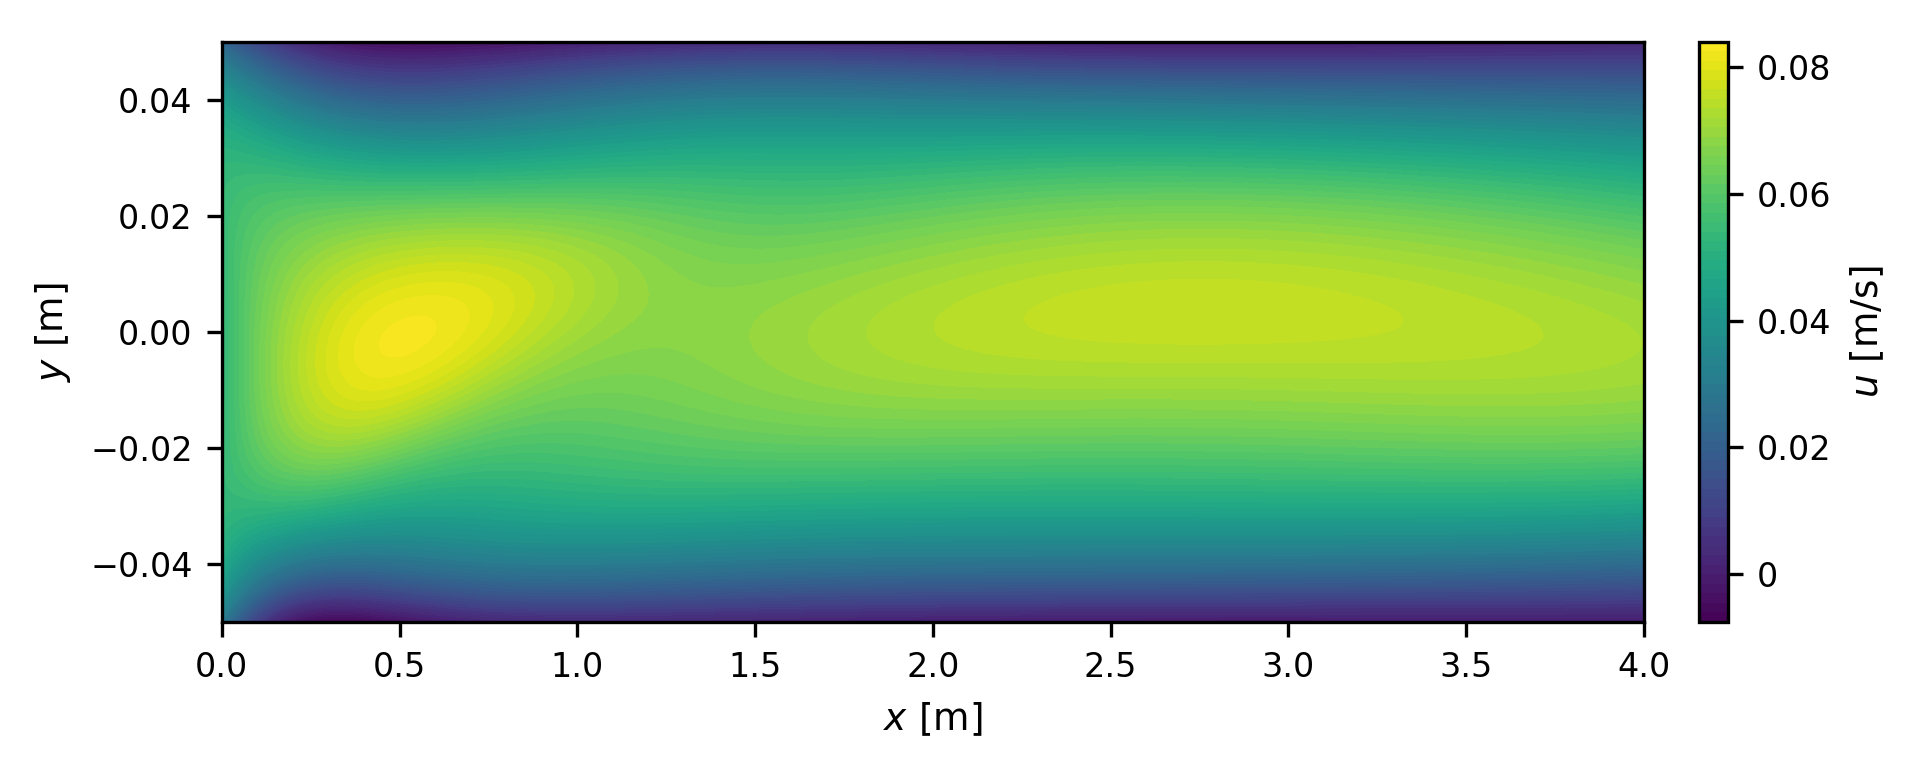
\includegraphics[width=\textwidth]{stage1_pred_u_Re100.png}
\caption{Streamwise velocity $u$ [m/s].}
\end{subfigure}
\hfill
\begin{subfigure}[b]{0.48\textwidth}
\centering
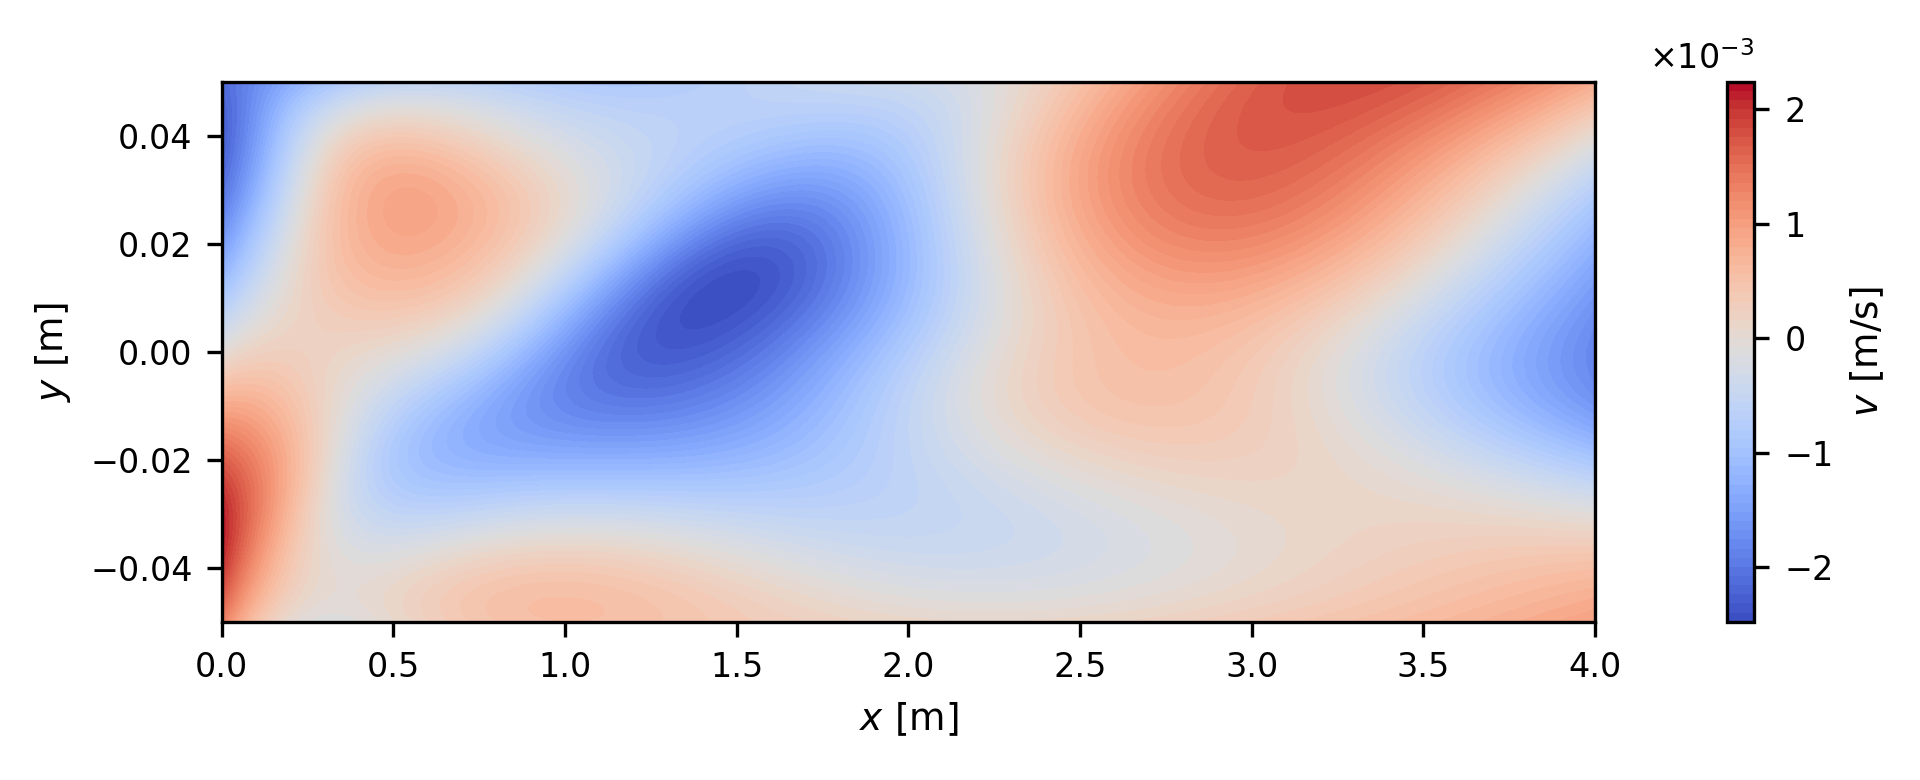
\includegraphics[width=\textwidth]{stage1_pred_v_Re100.png}
\caption{Transverse velocity $v$ [m/s].}
\end{subfigure}
\vskip\baselineskip
\begin{subfigure}[b]{0.48\textwidth}
\centering
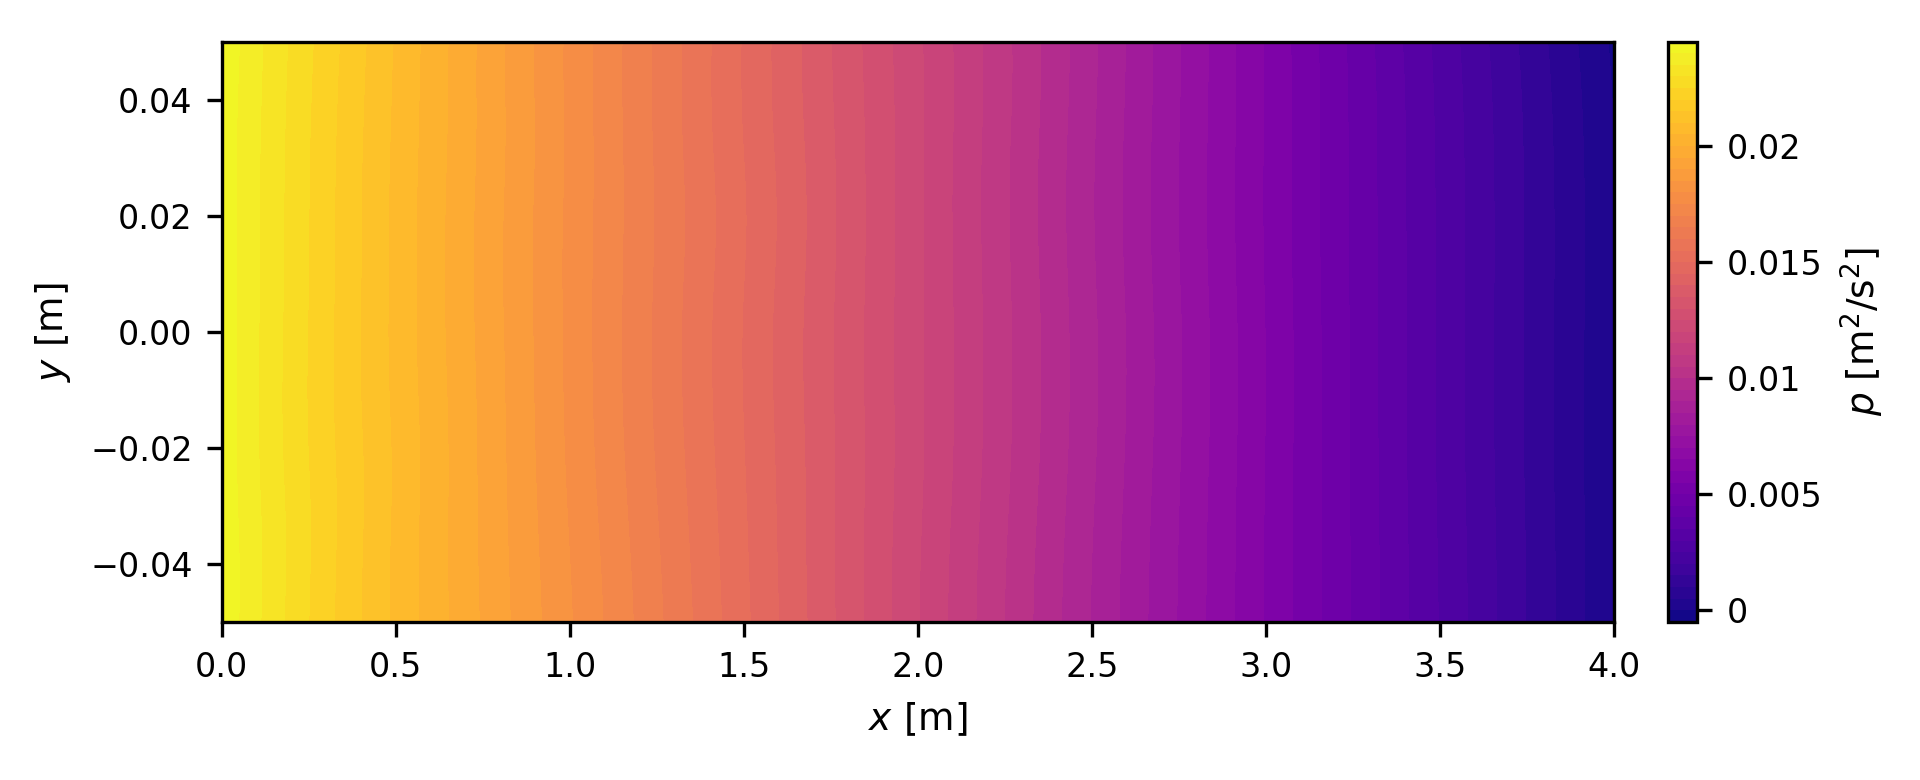
\includegraphics[width=\textwidth]{stage1_pred_p_Re100.png}
\caption{Kinematic pressure $p$ [$\mathrm{m^2/s^2}$].}
\end{subfigure}
\hfill
\begin{subfigure}[b]{0.48\textwidth}
\centering
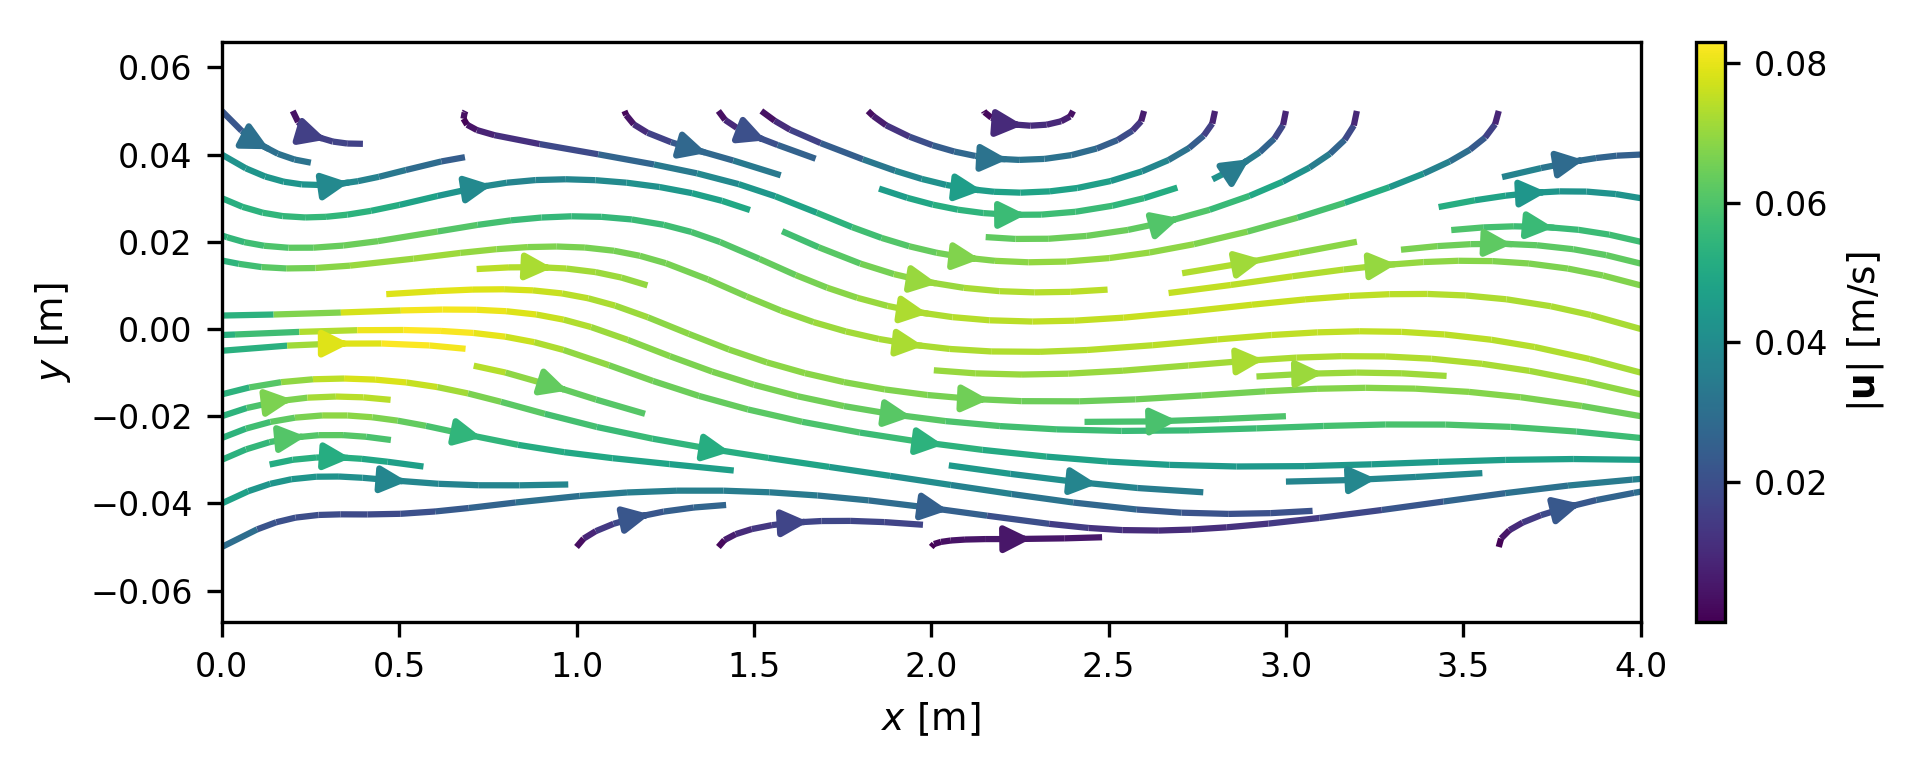
\includegraphics[width=\textwidth]{stage1_pred_streamlines_Re100.png}
\caption{Predicted streamlines colored by speed.}
\end{subfigure}
\caption{Stage 1: Predicted laminar flow fields at $\mathrm{Re} = 100$ (wall-normal axis stretched by a factor $k \approx 14$).}
\label{fig:stage1_pred_re100}
\end{figure}

\begin{figure}[H]
\centering
\begin{subfigure}[b]{0.48\textwidth}
\centering
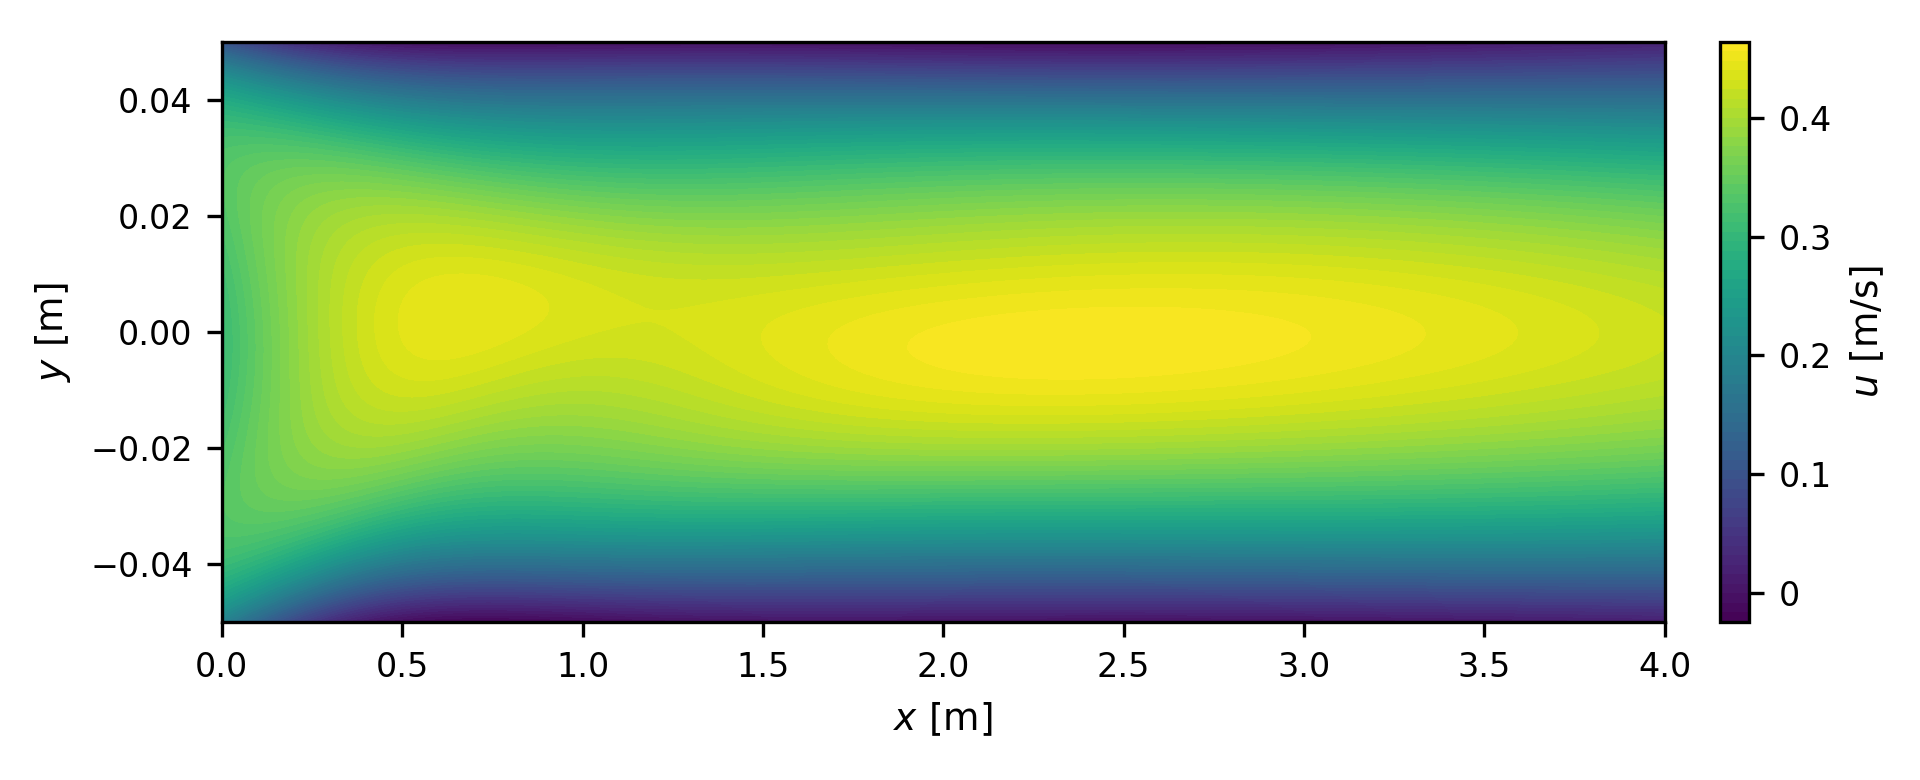
\includegraphics[width=\textwidth]{stage1_pred_u_Re600.png}
\caption{Streamwise velocity $u$ [m/s].}
\end{subfigure}
\hfill
\begin{subfigure}[b]{0.48\textwidth}
\centering
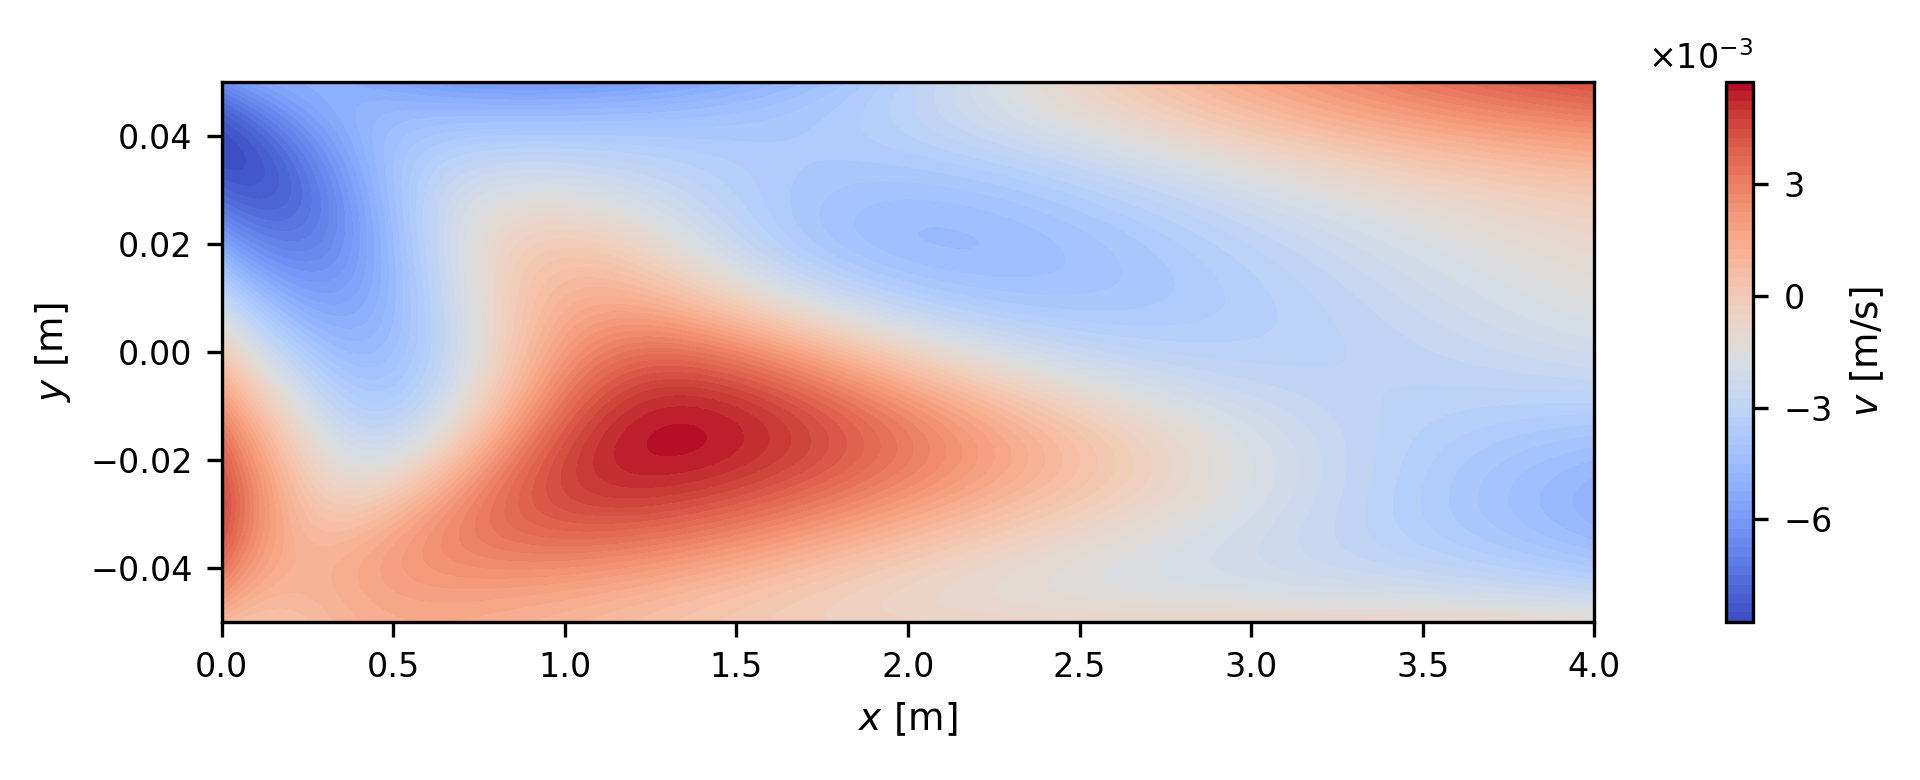
\includegraphics[width=\textwidth]{stage1_pred_v_Re600.png}
\caption{Transverse velocity $v$ [m/s].}
\end{subfigure}
\vskip\baselineskip
\begin{subfigure}[b]{0.48\textwidth}
\centering
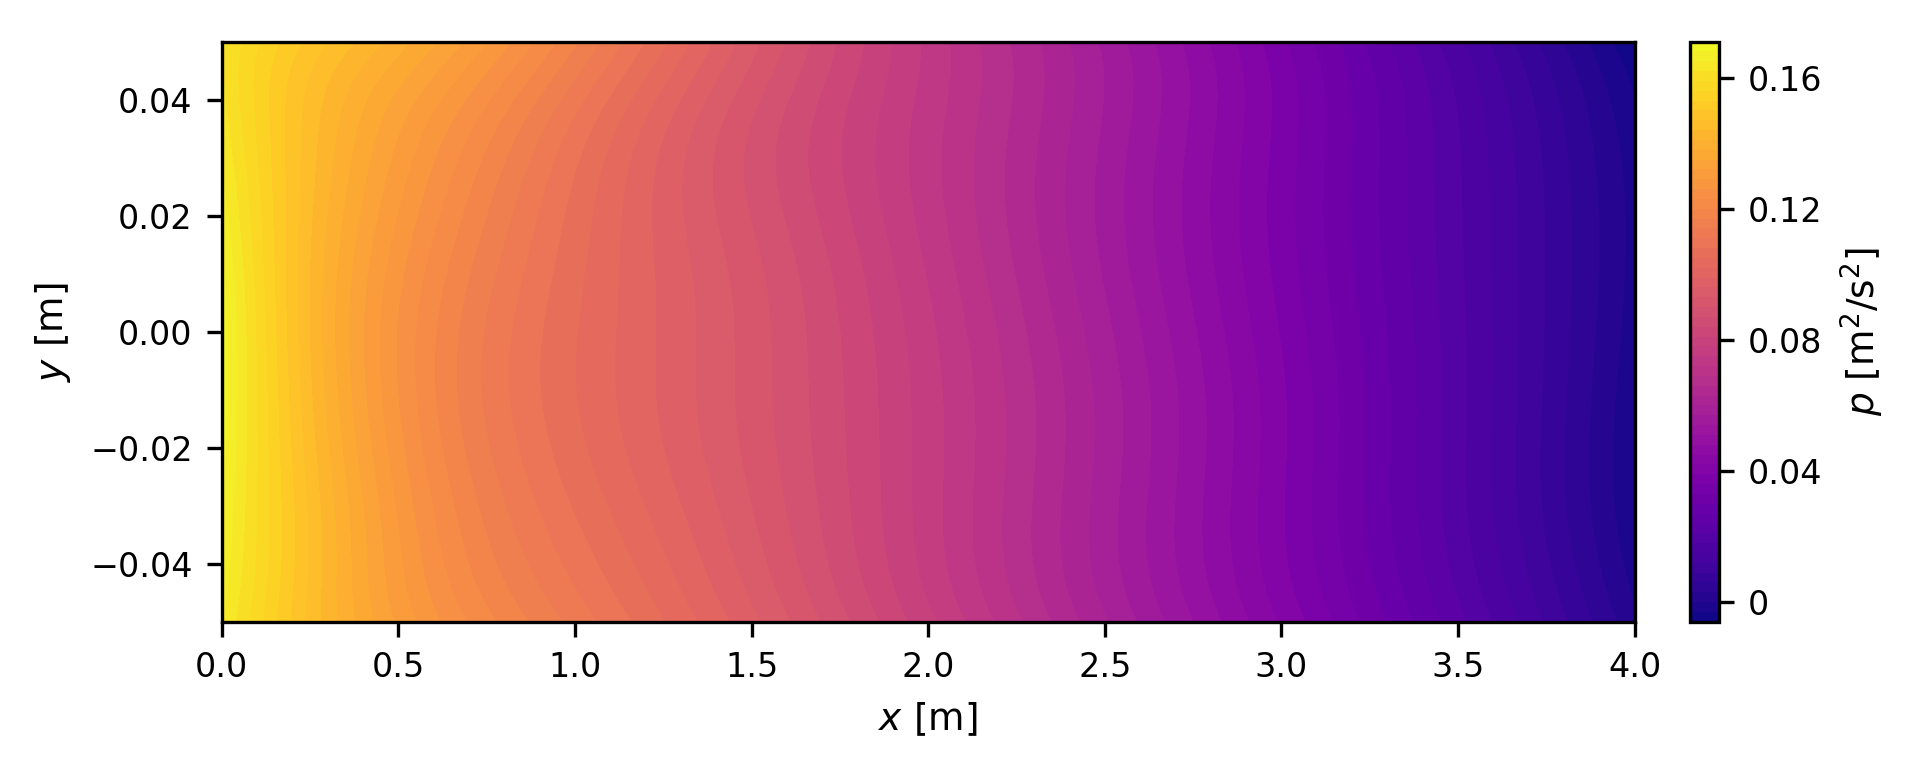
\includegraphics[width=\textwidth]{stage1_pred_p_Re600.png}
\caption{Kinematic pressure $p$ [$\mathrm{m^2/s^2}$].}
\end{subfigure}
\hfill
\begin{subfigure}[b]{0.48\textwidth}
\centering
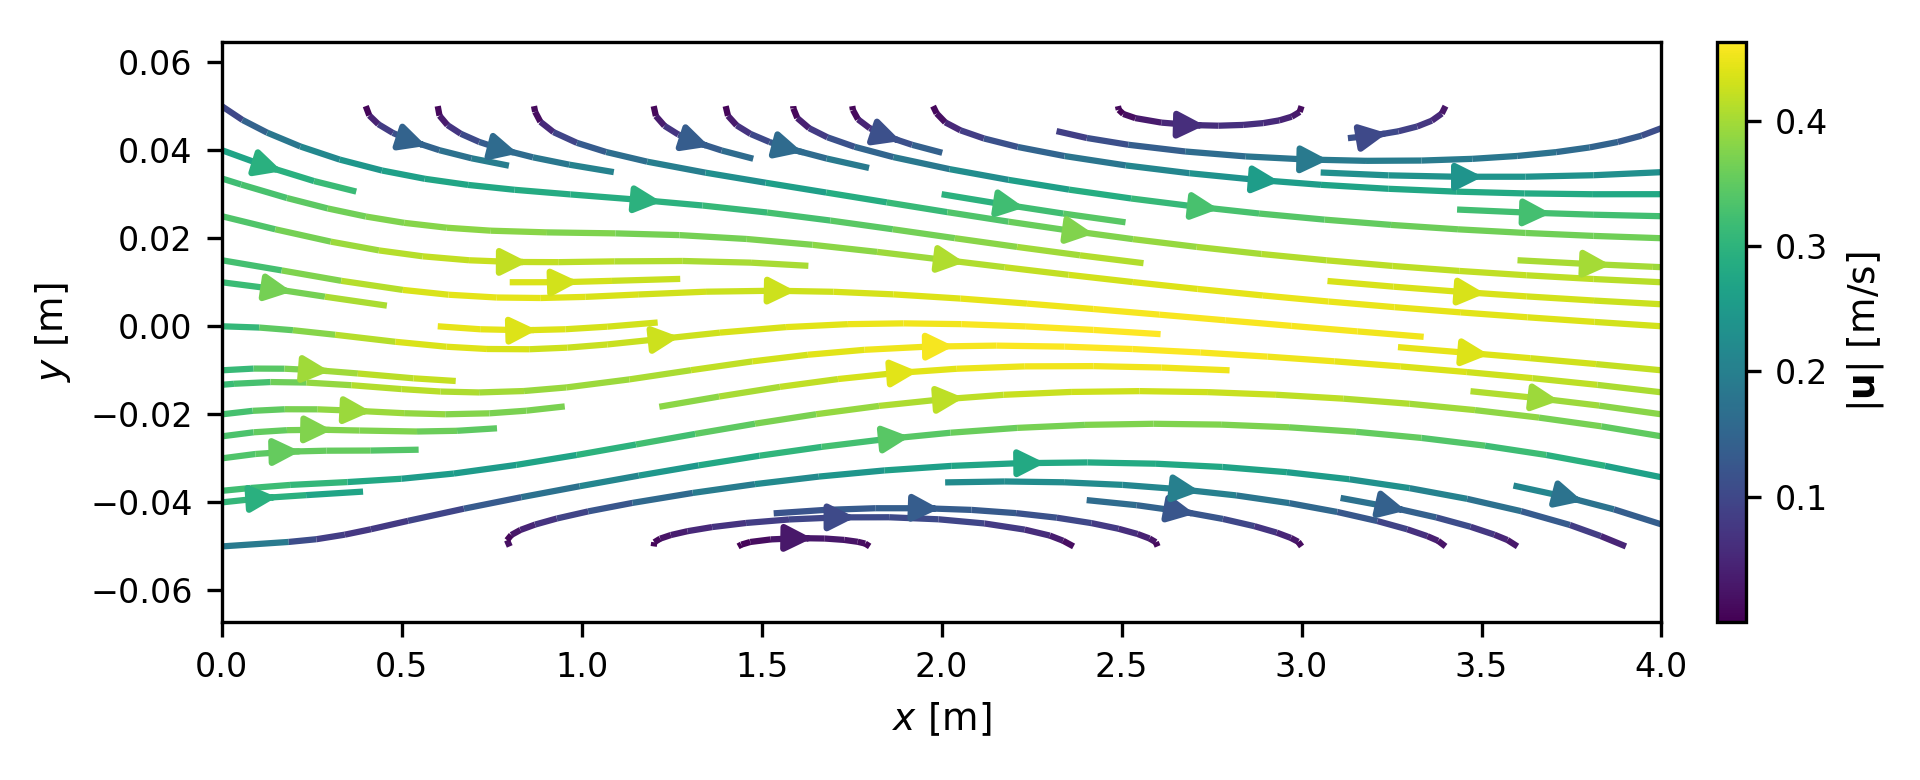
\includegraphics[width=\textwidth]{stage1_pred_streamlines_Re600.png}
\caption{Predicted streamlines colored by speed.}
\end{subfigure}
\caption{Stage 1: Predicted laminar flow fields at $\mathrm{Re} = 600$ (wall-normal axis stretched by a factor $k \approx 14$).}
\label{fig:stage1_pred_re600}
\end{figure}


\subsection{Discussion}
A limitation observed in Stage 1 is wall streamline deflection. Because boundary conditions are enforced via soft penalty loss ($\mathcal{L}_{\mathrm{wall}}$) rather than hard algebraic projection, small residual transverse velocities ($v \sim 10^{-4}\,\text{m/s}$) persist in near-wall cells. While dynamically small, near the wall where $u \to 0$, the streamline slope $dy/dx = v/u$ becomes non-zero, producing visible artificial streamline curvature near $y = \pm h$.

% ==============================================================================
% SECTION 4: STAGE 2
% ==============================================================================
\section{Stage 2: Laminar Axisymmetric Circular Pipe Flow}
\label{sec:stage2}

\subsection{Geometry and Physical Problem Setup}
Stage 2 investigates axisymmetric laminar entrance development in a circular pipe. The physical geometry is a straight circular tube of radius $R = 0.05\,\text{m}$, diameter $D = 2R = 0.10\,\text{m}$, and length $L = 4.0\,\text{m}$ ($L/D = 40$). Fluid kinematic viscosity is $\nu = 1.0\times 10^{-4}\,\text{m}^2/\text{s}$.

\begin{figure}[H]
\centering
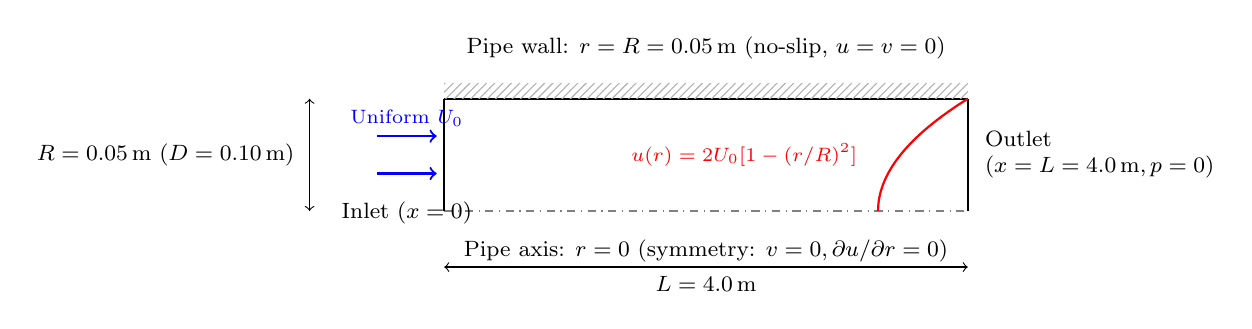
\begin{tikzpicture}[scale=0.95]
    \node[above, font=\footnotesize] at (3.5, 1.9) {Pipe wall: $r = R = 0.05\,\text{m}$ (no-slip, $u=v=0$)};
    \draw[thick] (0, 1.5) -- (7.0, 1.5);
    \fill[pattern=north east lines, pattern color=gray!60] (0, 1.5) rectangle (7.0, 1.7);
    \draw[dashdotted, thick, gray] (0, 0) -- (7.0, 0);
    \node[below, font=\footnotesize] at (3.5, -0.25) {Pipe axis: $r = 0$ (symmetry: $v=0, \partial u/\partial r = 0$)};
    \draw[thick] (0, 0) -- (0, 1.5);
    \draw[blue, thick, ->] (-0.9, 1.0) -- (-0.1, 1.0);
    \draw[blue, thick, ->] (-0.9, 0.5) -- (-0.1, 0.5);
    \node[blue, font=\scriptsize, above] at (-0.5, 1.0) {Uniform $U_0$};
    \node[font=\footnotesize, below] at (-0.5, 0.25) {Inlet ($x=0$)};
    \draw[thick] (7.0, 0) -- (7.0, 1.5);
    \node[right, font=\footnotesize, align=left] at (7.1, 0.75) {Outlet\\($x = L = 4.0\,\text{m}, p = 0$)};
    \draw[domain=0:1.5, smooth, variable=\y, red, thick] plot ({7.0 - 1.2*(1 - (\y/1.5)*(\y/1.5))}, {\y});
    \node[red, font=\scriptsize, fill=white, inner sep=2pt, left] at (5.6, 0.75) {$u(r) = 2 U_0 [1 - (r/R)^2]$};
    \draw[<->] (0, -0.75) -- (7.0, -0.75) node[midway, below, font=\footnotesize] {$L = 4.0\,\text{m}$};
    \draw[<->] (-1.8, 0) -- (-1.8, 1.5) node[midway, left=2pt, font=\footnotesize] {$R = 0.05\,\text{m}$ ($D = 0.10\,\text{m}$)};
\end{tikzpicture}
\caption{Stage 2 geometry: axisymmetric circular pipe entrance flow.}
\label{fig:stage2_geom}
\end{figure}

Due to swirl-free axisymmetry ($\partial/\partial\theta \equiv 0, u_\theta \equiv 0$), the flow is represented on the meridional half-plane $(x, r) \in [0, L] \times [0, R]$. The Reynolds number is $\mathrm{Re} = U_0 D / \nu \implies U_0(\mathrm{Re}) = 0.001\,\mathrm{Re}\,\text{m/s}$. Downstream, the profile converges to the Hagen--Poiseuille solution with peak centerline velocity $u_{\max} = 2 U_0$. At $\mathrm{Re}=100$, bulk velocity is $U_0 = 0.10\,\text{m/s}$, and the pressure scale is chosen as the total Hagen--Poiseuille viscous pressure drop over the pipe length $p_{\mathrm{scale}} = \frac{32 \nu U_0 L}{D^2} = 0.128\,\text{m}^2/\text{s}^2$.
% src: 2/model.py:51-53

\subsection{Governing Equations and Dimensionless Formulation}
The steady axisymmetric Navier--Stokes equations in cylindrical polar coordinates $(x, r)$ are:
\begin{align}
\frac{\partial u}{\partial x} + \frac{1}{r} \frac{\partial (r v)}{\partial r} &= 0, \\
u \frac{\partial u}{\partial x} + v \frac{\partial u}{\partial r} &= -\frac{\partial p}{\partial x} + \nu \left(\frac{\partial^2 u}{\partial x^2} + \frac{1}{r} \frac{\partial u}{\partial r} + \frac{\partial^2 u}{\partial r^2}\right), \\
u \frac{\partial v}{\partial x} + v \frac{\partial v}{\partial r} &= -\frac{\partial p}{\partial r} + \nu \left(\frac{\partial^2 v}{\partial x^2} + \frac{1}{r} \frac{\partial v}{\partial r} - \frac{v}{r^2} + \frac{\partial^2 v}{\partial r^2}\right).
\end{align}
To handle the geometric coordinate singularity at the axis ($r \to 0$), L'H\^opital's rule is applied at $r = 0$: $\lim_{r\to 0} (v/r) = \partial v/\partial r$, and $\lim_{r\to 0} (1/r)(\partial u/\partial r) = \partial^2 u/\partial r^2$.
% src: 2/config.py:34; chen1973; hornbeck1973
Hydrodynamic entrance length $L_e$ is estimated using the empirical correlation of Durst et al.~\cite[Eq.~(2a), p.~8]{ray2017}:
\begin{equation}
\frac{L_e}{D} = \left[(0.619)^{1.6} + (0.0567\,\mathrm{Re})^{1.6}\right]^{1/1.6}.
\end{equation}
At $D = 0.10\,\text{m}$, the correlation gives $L_e = 0.577\,\text{m}$ at $\mathrm{Re}=100$, $1.706\,\text{m}$ at $\mathrm{Re}=300$, and $3.405\,\text{m}$ at $\mathrm{Re}=600$, all within the pipe length $L = 4.0\,\text{m}$.

\subsection{Reference Solver and Discretization}
Reference data was computed on a $500 \times 81$ grid using a circular pipe marching finite-difference solver based on Hornbeck~\cite[Ch.~7, pp.~195--202]{hornbeck1973} (\texttt{2/entrance\_solver.py}).
The solver solves the parabolized axisymmetric boundary-layer equations:
\begin{align}
u \frac{\partial u}{\partial x} + v \frac{\partial u}{\partial r} &= -\frac{1}{\rho}\frac{dP}{dx} + \nu \frac{1}{r}\frac{\partial}{\partial r}\left(r \frac{\partial u}{\partial r}\right), \\
\frac{\partial u}{\partial x} + \frac{1}{r}\frac{\partial (r v)}{\partial r} &= 0.
\end{align}
The solver drops streamwise diffusion ($\partial^2 u/\partial x^2 = 0$) and drops radial momentum ($\partial p/\partial r = 0 \implies p = p(x)$). Global mass conservation $2\pi \int_0^R u r\,dr = \pi R^2 U_0$ is enforced via superposition at each axial step.

As noted in Section~\ref{sec:elliptic_vs_parabolic}, the network is trained on the full axisymmetric Navier--Stokes equations whereas the reference solver neglects axial diffusion and the radial pressure gradient; the resulting difference is largest near the inlet.

\subsection{Network Design and Hyperparameters}
The Stage 2 network (\texttt{2/model.py}, class \texttt{PipePINN}) is an MLP with four hidden layers of 80 neurons with $\tanh$ activations ($[3, 80, 80, 80, 80, 3]$, 20,003 parameters). Inputs are normalized coordinates:
\begin{equation}
\hat{x} = \frac{x}{L} \in [0, 1], \quad \hat{r} = \frac{r}{R} \in [0, 1], \quad \mathrm{Re}_n = 2\frac{\log_{10}(\mathrm{Re}/50)}{\log_{10}(500/50)} - 1 \in [-1, 1].
\end{equation}
Training uses Adam for 2500 iterations (learning rate $8.0\times 10^{-4}$, StepLR $\gamma=0.7$ every 400 steps) followed by 300 iterations of L-BFGS polish. At each iteration, $N_{\mathrm{data}} = 200$ reference points are drawn randomly from the reference solution, and $N_{\mathrm{pde}} = 1{,}500$ interior points are drawn anew with area-weighted radial distribution ($r = R\sqrt{u}$) and inlet clustering in $x$. Collocation counts are 200 data points, 1,500 interior points, and 150 boundary points.

\subsection{Loss Formulation and Final Loss Weights}
The composite loss function incorporates six terms:
\begin{equation}
\mathcal{L} = w_{\mathrm{data}}\mathcal{L}_{\mathrm{data}} + w_{\mathrm{pde}}\mathcal{L}_{\mathrm{pde}} + w_{\mathrm{inlet}}\mathcal{L}_{\mathrm{inlet}} + w_{\mathrm{wall}}\mathcal{L}_{\mathrm{wall}} + w_{\mathrm{axis}}\mathcal{L}_{\mathrm{axis}} + w_{\mathrm{outlet}}\mathcal{L}_{\mathrm{outlet}}.
\end{equation}
The supervised data loss normalizes velocities by $U_0$ and pressure by $p_{\mathrm{scale}} = \frac{32\nu U_0 L}{D^2} = 0.128\,\text{m}^2/\text{s}^2$:
% src: 2/train_hybrid.py:180-183; 2/model.py:51
\begin{equation}
\mathcal{L}_{\mathrm{data}} = \frac{1}{N_d}\sum_{i=1}^{N_d} \left[ \left(\frac{u_i - u_i^{\mathrm{ref}}}{U_0}\right)^2 + \left(\frac{v_i - v_i^{\mathrm{ref}}}{U_0}\right)^2 + 0.1\left(\frac{p_i - p_i^{\mathrm{ref}}}{p_{\mathrm{scale}}}\right)^2 \right].
\end{equation}
(The pressure term carries a sub-weight of $0.1$ in \path{2/train_hybrid.py} because the marching finite-difference pressure is noisier than the velocity fields.)

The axis symmetry penalty is $\mathcal{L}_{\mathrm{axis}} = \frac{1}{N_{\mathrm{ax}}}\sum (v_k/U_0)^2$.

The final loss weights read from \texttt{2/train\_hybrid.py} are:
\begin{equation}
% src: 2/train_hybrid.py Line 40
w_{\mathrm{data}} = 10.0, \quad w_{\mathrm{pde}} = 1.0, \quad w_{\mathrm{inlet}} = 5.0, \quad w_{\mathrm{wall}} = 5.0, \quad w_{\mathrm{axis}} = 5.0, \quad w_{\mathrm{outlet}} = 5.0.
\end{equation}
The relative physics-to-data loss weight ratio is $w_{\mathrm{pde}} / w_{\mathrm{data}} = 1.0 / 10.0 = \mathbf{0.10}$.

\subsection{Forward Pass at a Single Point}
The pre-activation vector $z = W a_{\mathrm{prev}} + b$ represents the affine combination entering each layer, while the post-activation $a = \tanh(z)$ is its bounded output. Matrix $\|W\|_F$ denotes the Frobenius norm of the layer weight matrix, $\|b\|_2$ is the Euclidean norm of the bias vector, and $z[1:4]$ reports the numerical values of the first four neurons of each layer.

Table~\ref{tab:stage2_act} presents the forward pass evaluated from \texttt{2/outputs/pipe\_pinn\_hybrid.pt} at $(x=2.0\,\text{m}, r=0.02\,\text{m}, \mathrm{Re}=100)$.
\begin{table}[H]
\centering
\small
\begin{tabular}{lcccc}
\toprule
\textbf{Network Layer} & \textbf{Pre-activations} $z_{[1:4]}$ & \textbf{Post-activations} $a_{[1:4]} = \tanh(z)$ & $\|W\|_F$ & $\|b\|_2$ \\
\midrule
Hidden 1 & $[0.1764, -0.3400, 0.0085, 0.1776]$ & $[0.1746, -0.3275, 0.0085, 0.1757]$ & 3.31 & 0.68 \\
Hidden 2 & $[0.5674, -0.2786, 0.2018, -0.1915]$ & $[0.5134, -0.2716, 0.1991, -0.1892]$ & 9.56 & 0.59 \\
Hidden 3 & $[-0.6102, -0.6115, 1.2029, 0.4668]$ & $[-0.5443, -0.5452, 0.8345, 0.4356]$ & 9.82 & 0.55 \\
Hidden 4 & $[0.6164, 0.5897, -0.8559, -0.1174]$ & $[0.5486, 0.5297, -0.6942, -0.1168]$ & 9.74 & 0.38 \\
Output & $[1.6939, 0.0311, -0.5011]$ & N/A & 3.47 & 0.11 \\
\bottomrule
\end{tabular}
\caption{Deterministic layer-by-layer forward pass evaluated at $(x=2.0\,\text{m}, r=0.02\,\text{m}, \mathrm{Re}=100)$. Normalized input vector: $[0.5000, 0.4000, -0.3979]^{\mathsf T}$. Checkpoint SHA256: \texttt{d266c592d74a24a9...}.}
\label{tab:stage2_act}
\end{table}
Normalized inputs are $[0.500, 0.400, -0.3979]$. With $U_0 = 0.10\,\text{m/s}$ and total viscous pressure drop scale $p_{\mathrm{scale}} = \frac{32 \nu U_0 L}{D^2} = 0.128\,\text{m}^2/\text{s}^2$ (Hagen--Poiseuille scale), physical predictions are:
\begin{align}
% src: 2/model.py:73; 2/outputs/reference_data.npz
u &= 1.6939 \times 0.10 = \mathbf{0.16939\,\text{m/s}} \quad (\text{reference: } 0.16803\,\text{m/s}, \text{ error } 0.81\%), \\
v &= 0.0311 \times 0.10 = \mathbf{0.00311\,\text{m/s}} \quad (\text{reference: } -1.30\times 10^{-8}\,\text{m/s}), \\
p &= -0.5011 \times 0.128 = \mathbf{-0.06414\,\text{m}^2/\text{s}^2} \quad (\text{reference gauge: } -0.06401\,\text{m}^2/\text{s}^2, \text{ error } 0.20\%).
\end{align}

\subsection{Empirical Results and Performance Evaluation}
Table~\ref{tab:stage2_metrics} reports quantitative errors ordered monotonically by Reynolds number ($\mathrm{Re} = 50$, $100$, $200$, $300$, $500$, and $600$).
\begin{table}[H]
\centering
\resizebox{\textwidth}{!}{
\begin{tabular}{lcccccc}
\toprule
\textbf{Metric Variable} & $\mathbf{Re=50}$ & $\mathbf{Re=100}$ & $\mathbf{Re=200}$ & $\mathbf{Re=300}$ (TEST-interp) & $\mathbf{Re=500}$ & $\mathbf{Re=600}$ (TEST-extrap) \\
\midrule
$u$ (Axial Velocity Rel $L_2$) & 2.65\% & 2.20\% & 2.80\% & 3.24\% & 3.86\% & 4.16\% \\
$v$ (Radial Velocity Rel $L_2$) & 4.25\% & 2.94\% & 1.85\% & 1.35\% & 0.93\% & 0.85\% \\
$p$ (Kinematic Pressure Rel $L_2$) & 2.76\% & 1.56\% & 1.36\% & 1.47\% & 1.84\% & 2.40\% \\
\bottomrule
\end{tabular}
}
\caption{Stage 2: Full-domain relative $L_2$ errors for axisymmetric circular pipe flow (Source: \texttt{2/outputs/metrics\_global.csv}).}
\label{tab:stage2_metrics}
\end{table}


\begin{figure}[H]
\centering
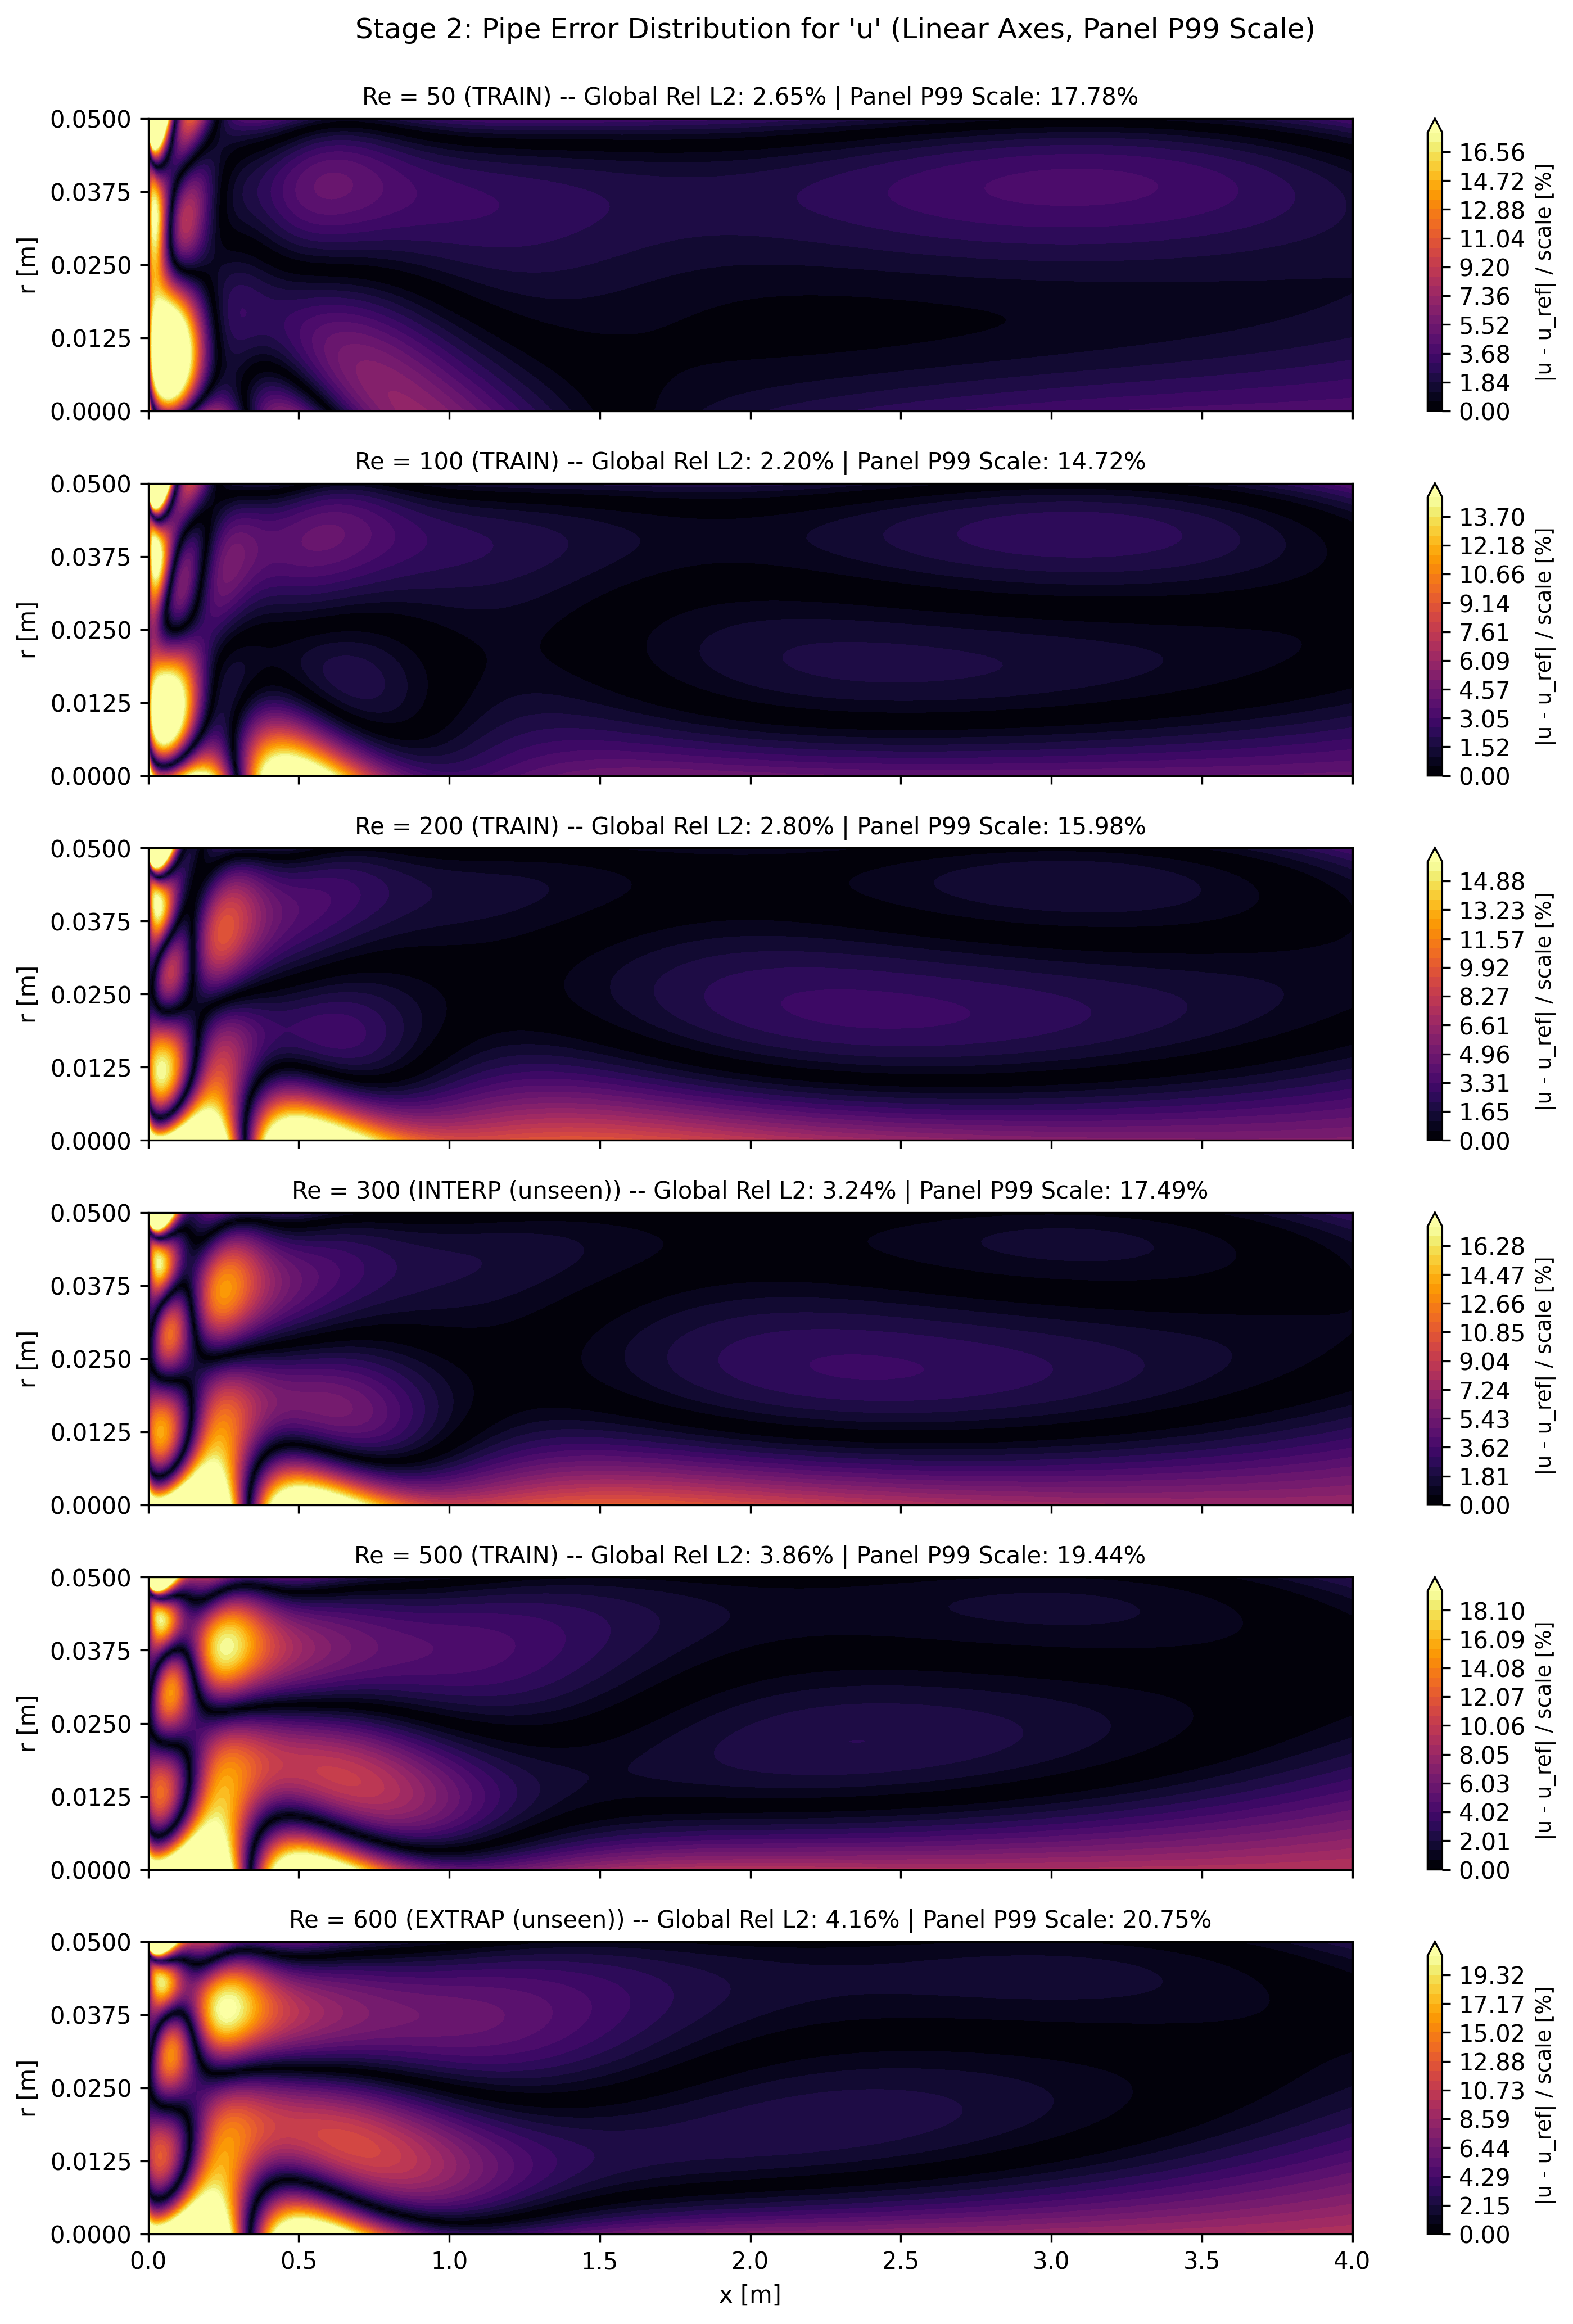
\includegraphics[width=0.95\textwidth]{stage2_error_u.png}
\caption{Stage 2: Axisymmetric axial velocity error $|u - u_{\mathrm{ref}}|/U_0$ [\%] across the Reynolds sweep.}
\label{fig:stage2_errors}
\end{figure}

\begin{figure}[H]
\centering
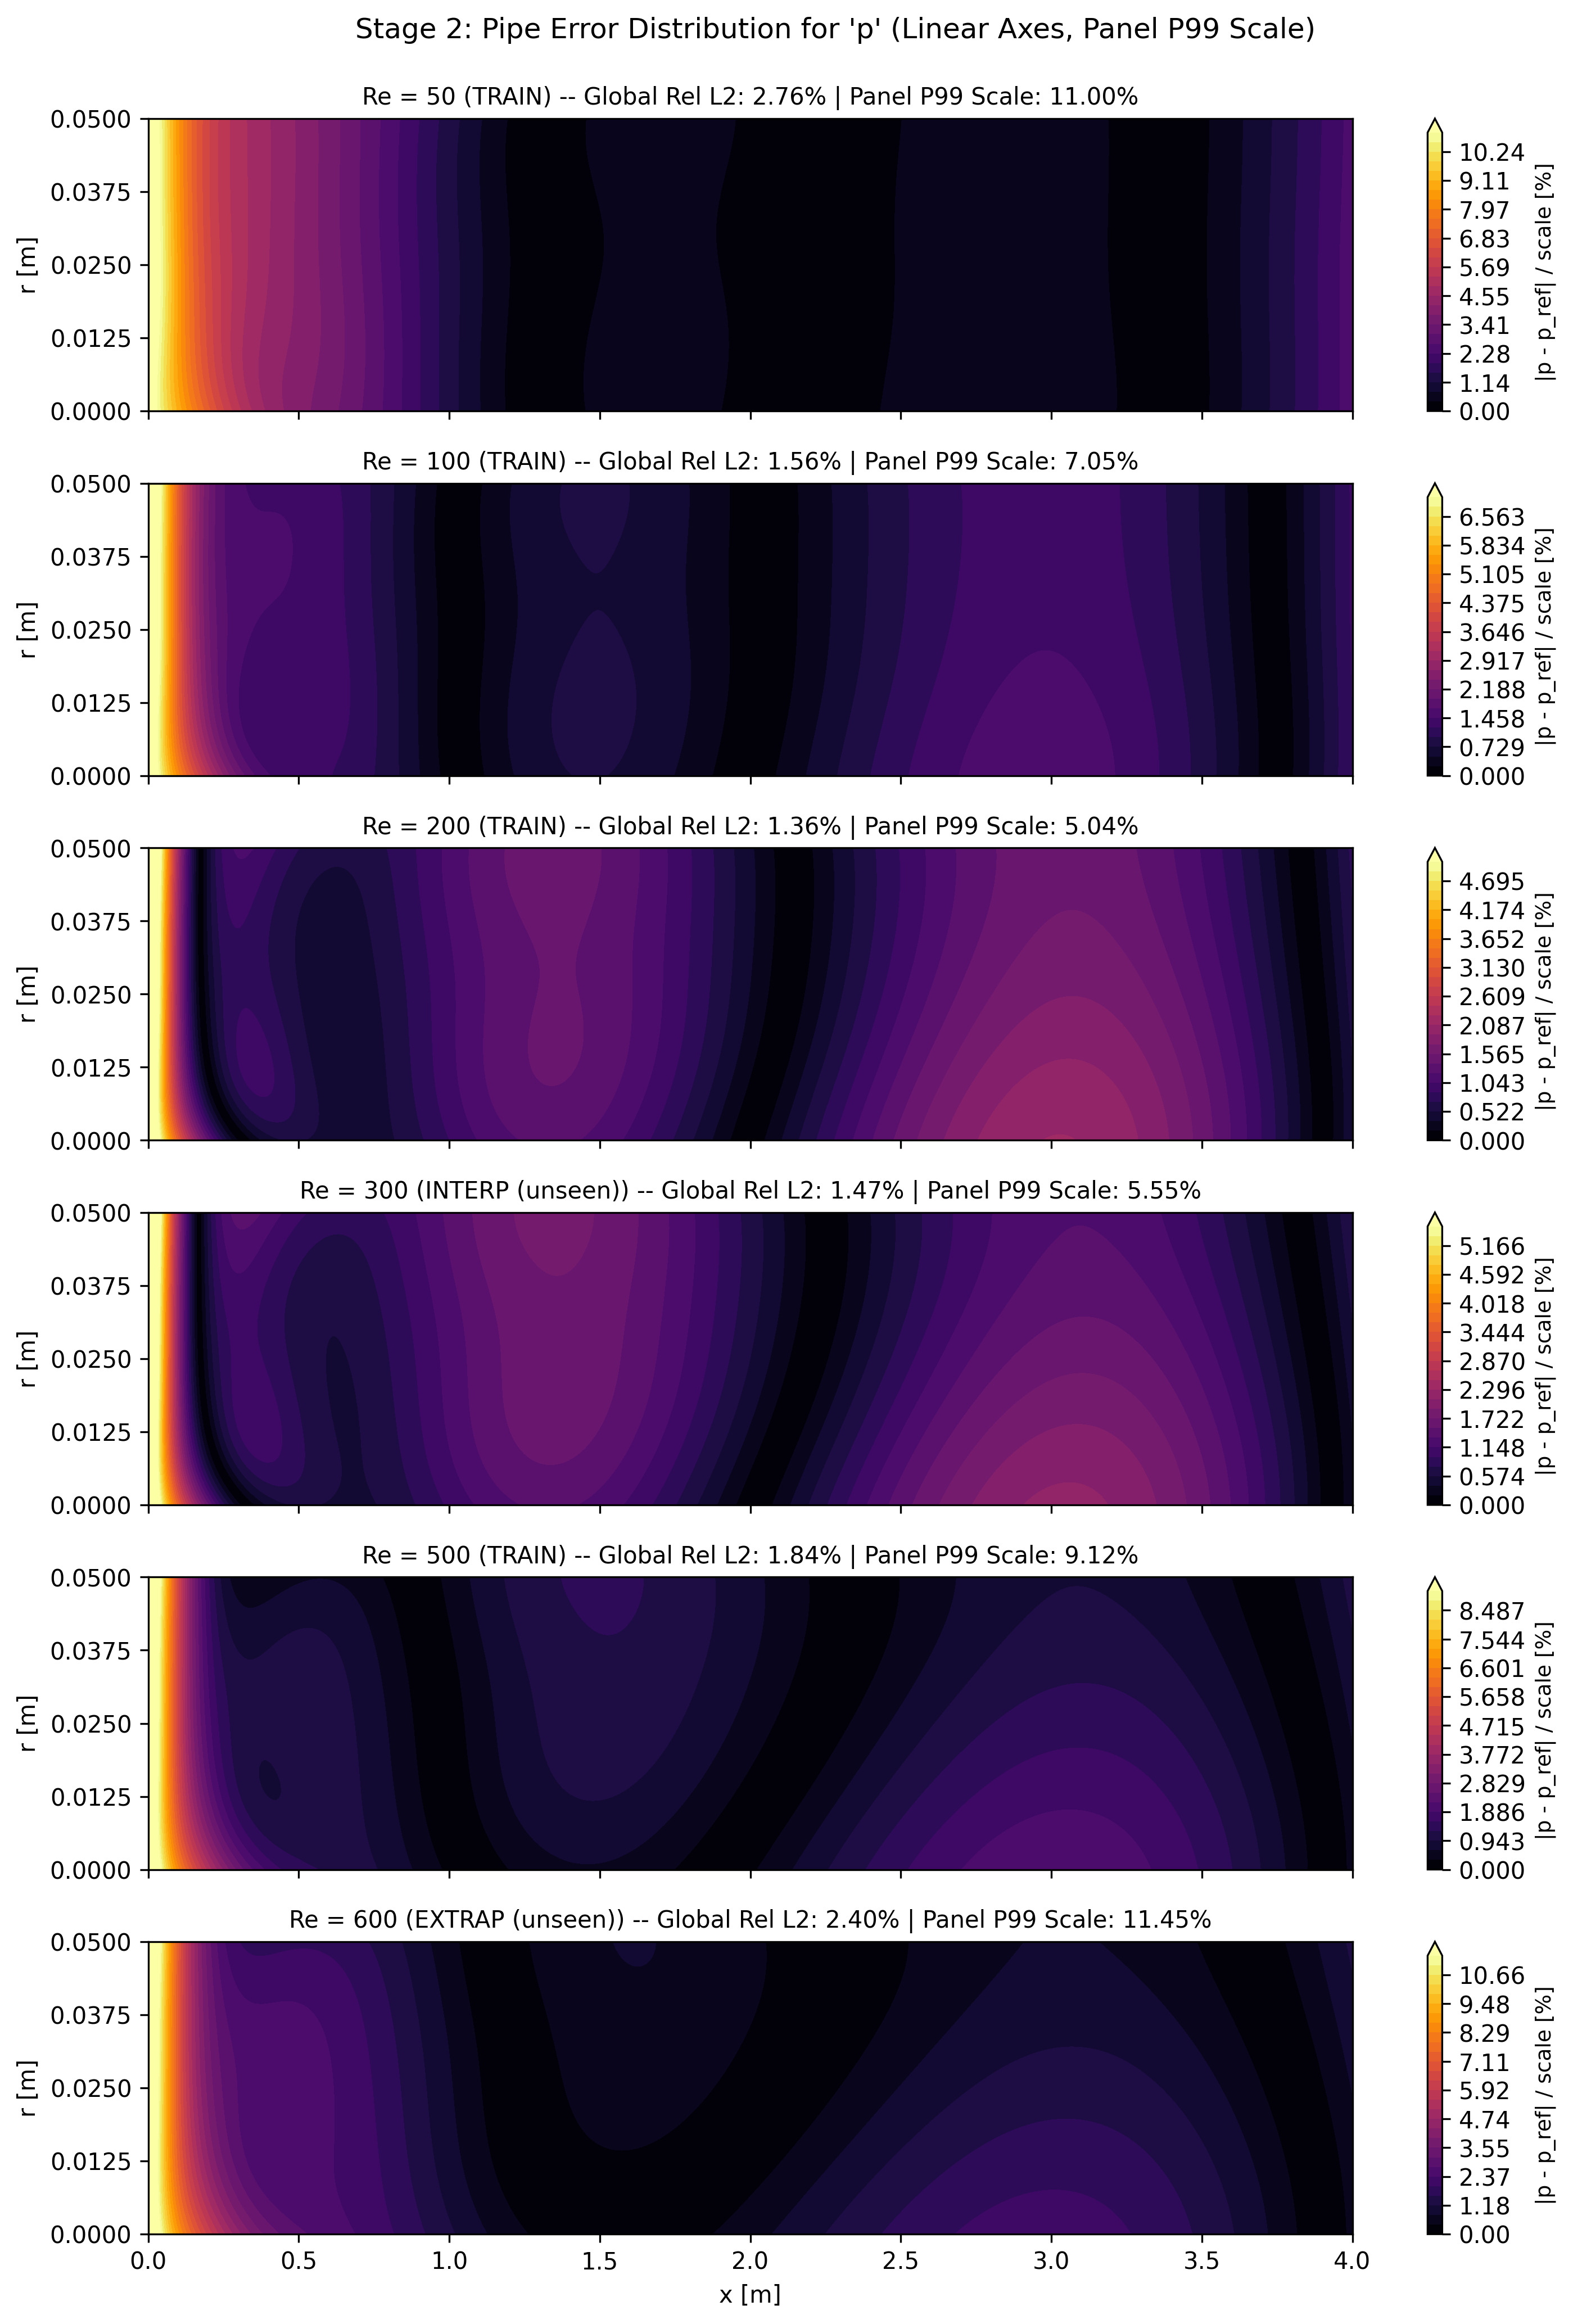
\includegraphics[width=0.95\textwidth]{stage2_error_p.png}
\caption{Stage 2: Kinematic pressure error $|p - p_{\mathrm{ref}}|/p_{\mathrm{scale}}$ [\%] across the Reynolds sweep.}
\label{fig:stage2_error_p}
\end{figure}

\noindent\textbf{Interpretation of Results:}
% src: 2/outputs/metrics_summary.json; 2/outputs/reference_data.npz
The circular pipe achieves lower velocity errors than the 2D channel ($2.20\%$--$4.16\%$ vs.\ $3.88\%$--$5.69\%$). Pointwise median errors range from $1.11\%$ to $2.13\%$, with 95th percentiles (P95) between $4.42\%$ and $11.54\%$. Area-weighted radial sampling ($dA = 2\pi r\,dr$) concentrates collocation points towards the pipe wall, providing denser resolution across the developing shear layer. Pressure relative $L_2$ errors remain below $2.76\%$. 


\subsection{Predicted Flow Fields}
Figures~\ref{fig:stage2_pred_re100} and~\ref{fig:stage2_pred_re600} display the predicted axisymmetric pipe flow fields ($L=4.0\,\text{m}$, $R=0.05\,\text{m}$, $L/R=80$) at $\mathrm{Re} = 100$ and $600$. The radial coordinate is stretched by a factor $k \approx 29$ relative to the physical aspect ratio for visual clarity.

Axial velocity $u_x$ develops smoothly from the uniform entrance condition to the quadratic Poiseuille profile along the pipe center. Radial velocity $u_r$ exhibits a localized inward flux near the inlet to accommodate boundary-layer displacement, diminishing to zero as the flow approaches the fully developed state. Streamlines demonstrate smooth parallel flow downstream, with monotonic axial pressure dissipation.

\begin{figure}[H]
\centering
\begin{subfigure}[b]{0.48\textwidth}
\centering
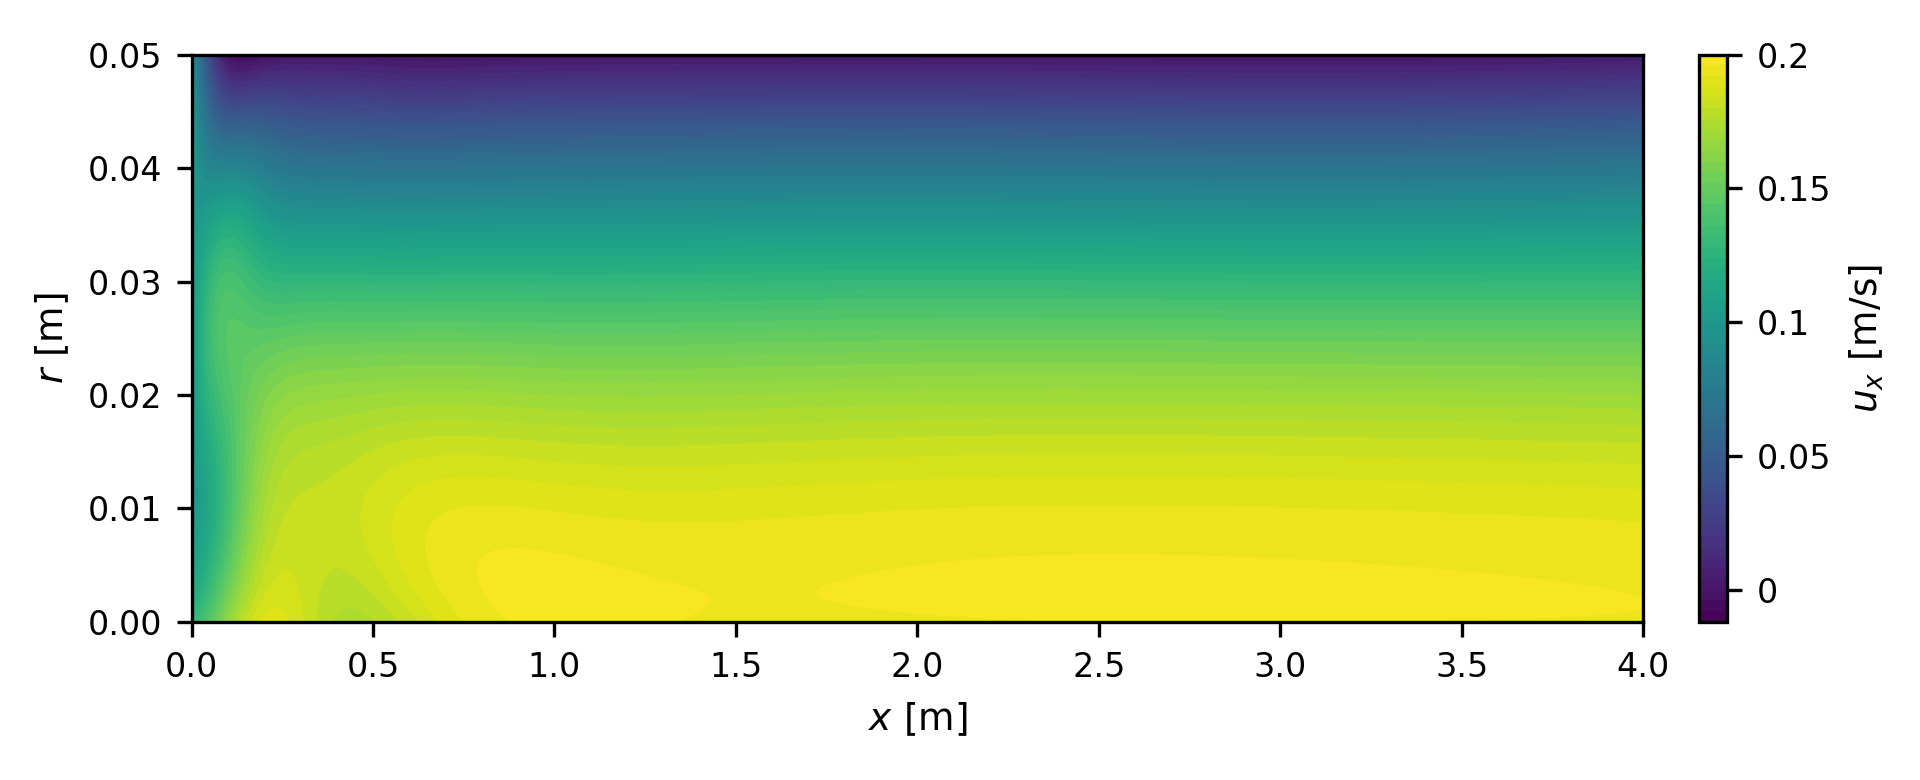
\includegraphics[width=\textwidth]{stage2_pred_ux_Re100.png}
\caption{Axial velocity $u_x$ [m/s].}
\end{subfigure}
\hfill
\begin{subfigure}[b]{0.48\textwidth}
\centering
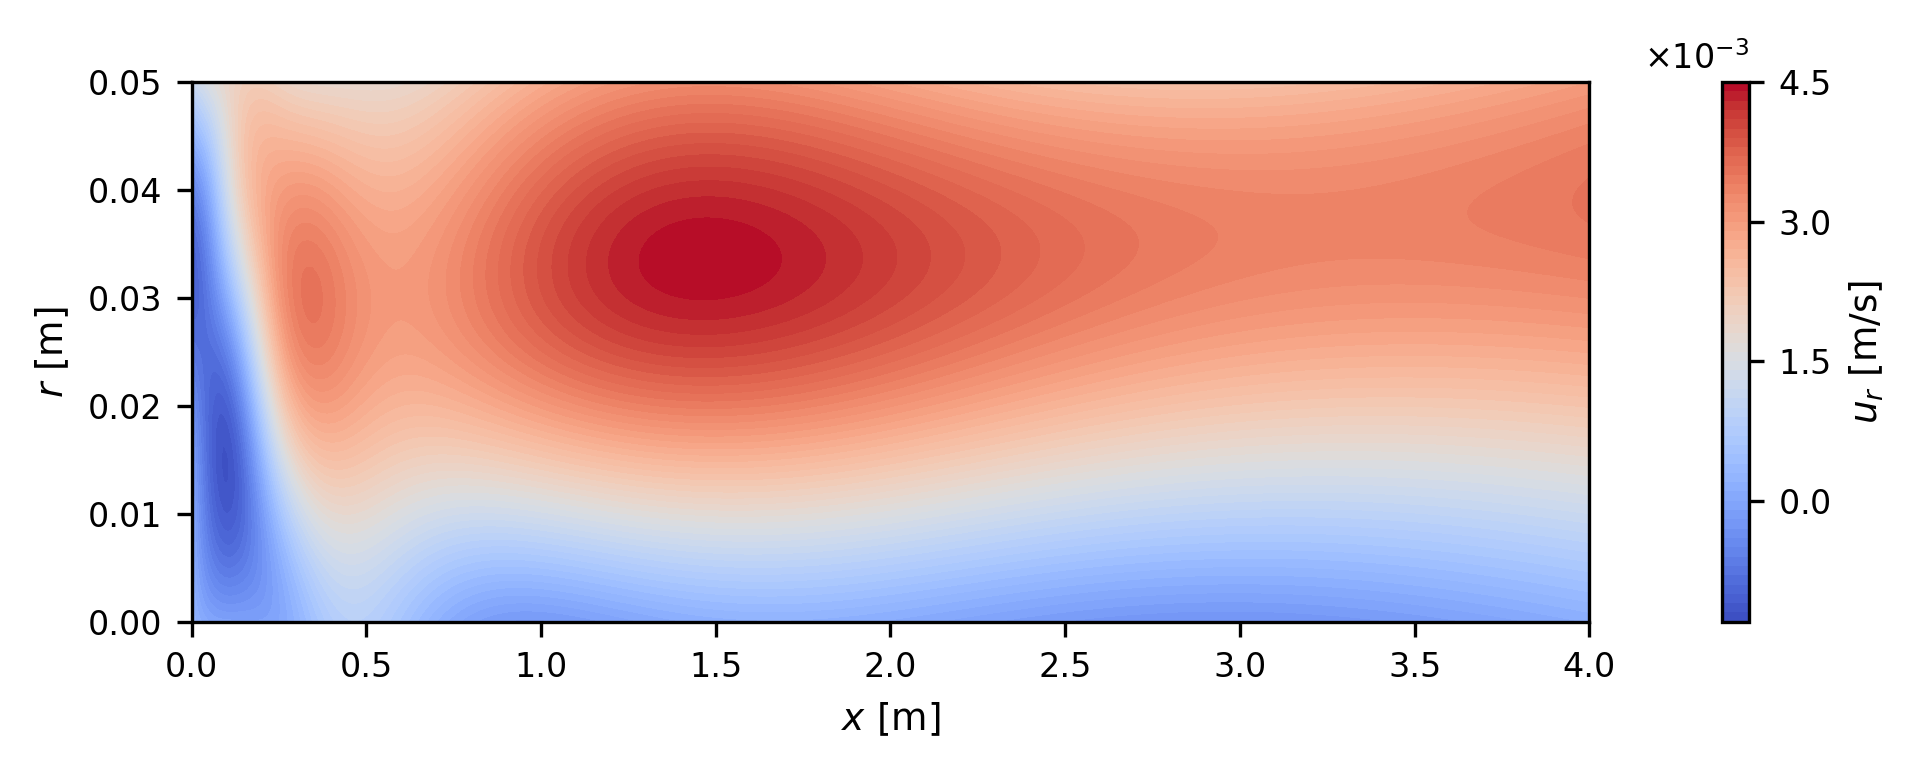
\includegraphics[width=\textwidth]{stage2_pred_ur_Re100.png}
\caption{Radial velocity $u_r$ [m/s].}
\end{subfigure}
\vskip\baselineskip
\begin{subfigure}[b]{0.48\textwidth}
\centering
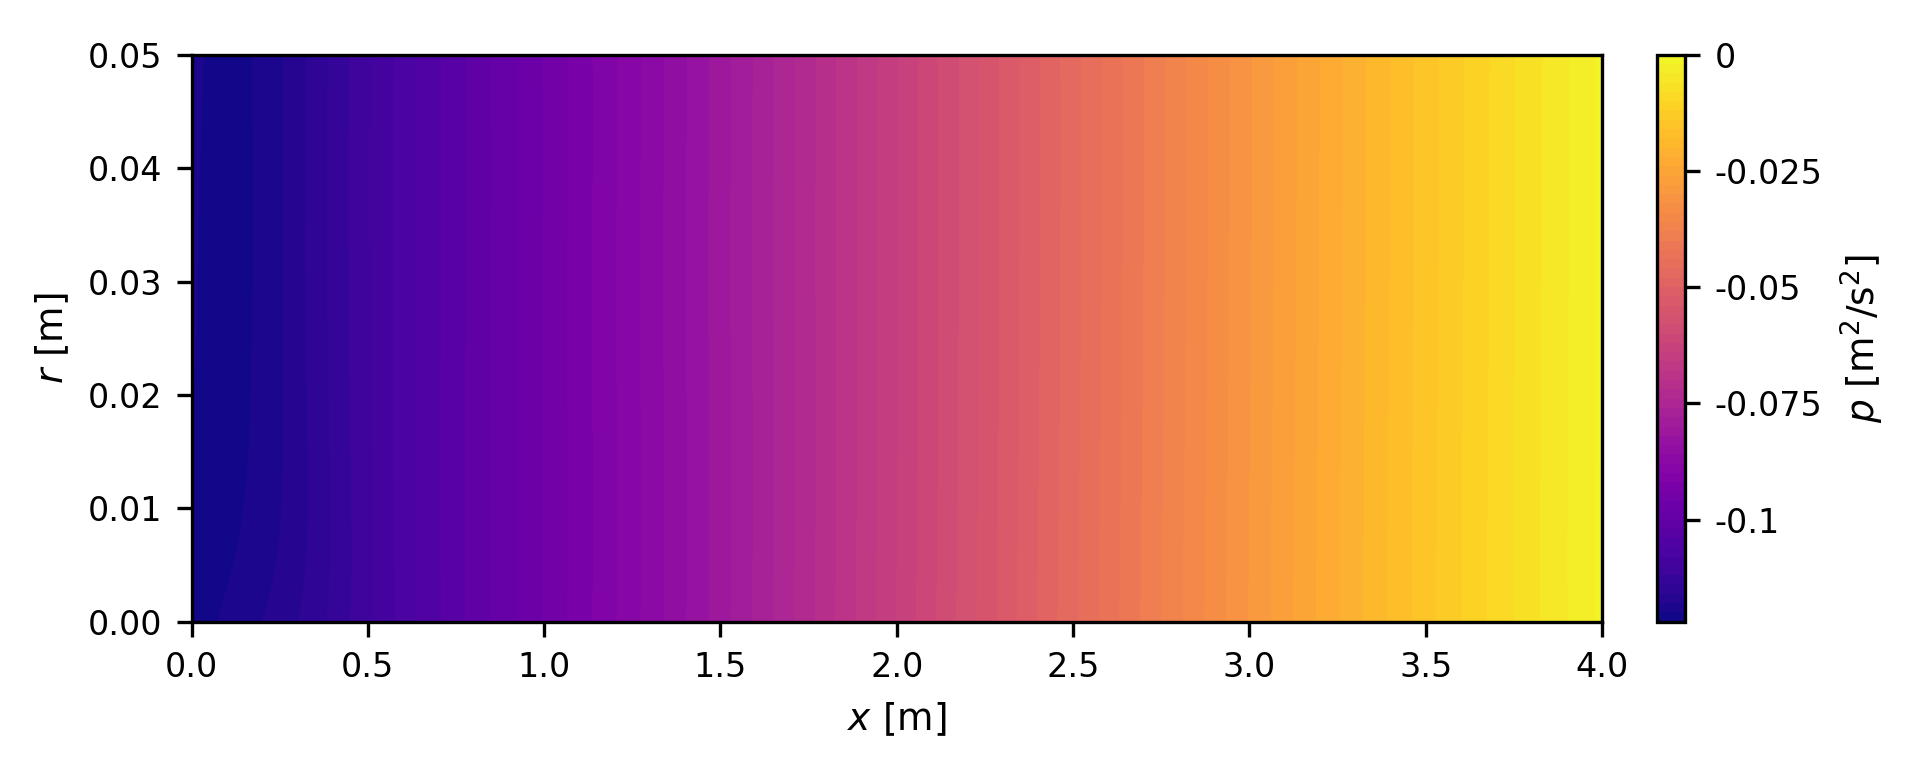
\includegraphics[width=\textwidth]{stage2_pred_p_Re100.png}
\caption{Kinematic pressure $p$ [$\mathrm{m^2/s^2}$].}
\end{subfigure}
\hfill
\begin{subfigure}[b]{0.48\textwidth}
\centering
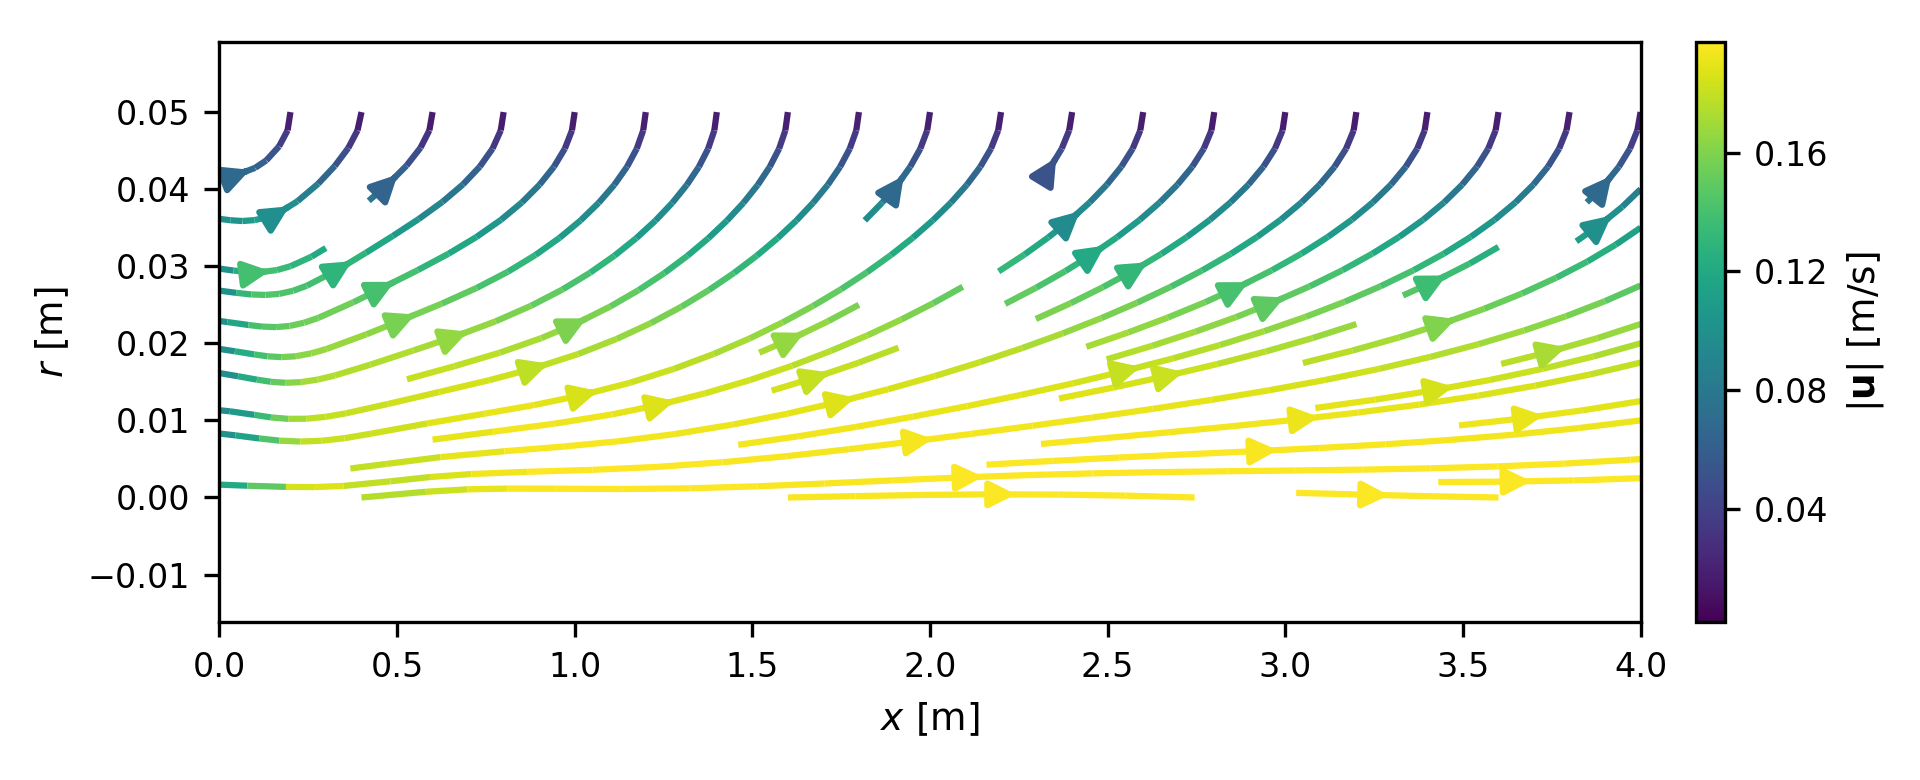
\includegraphics[width=\textwidth]{stage2_pred_streamlines_Re100.png}
\caption{Predicted streamlines colored by speed.}
\end{subfigure}
\caption{Stage 2: Predicted laminar pipe flow fields at $\mathrm{Re} = 100$ (radial axis stretched by a factor $k \approx 29$).}
\label{fig:stage2_pred_re100}
\end{figure}

\begin{figure}[H]
\centering
\begin{subfigure}[b]{0.48\textwidth}
\centering
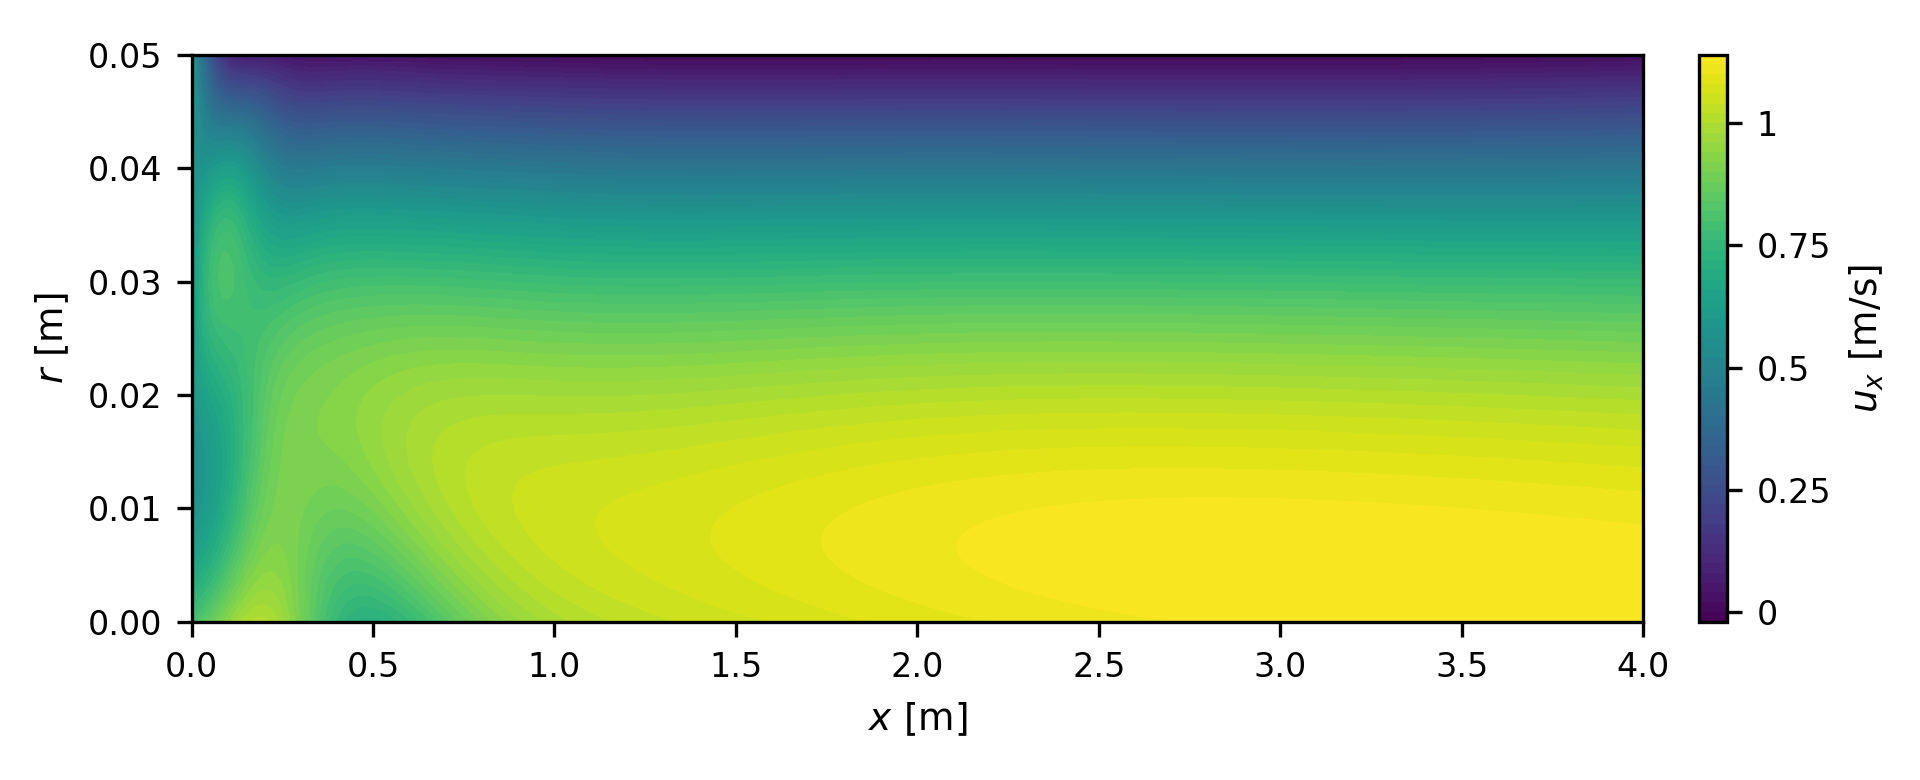
\includegraphics[width=\textwidth]{stage2_pred_ux_Re600.png}
\caption{Axial velocity $u_x$ [m/s].}
\end{subfigure}
\hfill
\begin{subfigure}[b]{0.48\textwidth}
\centering
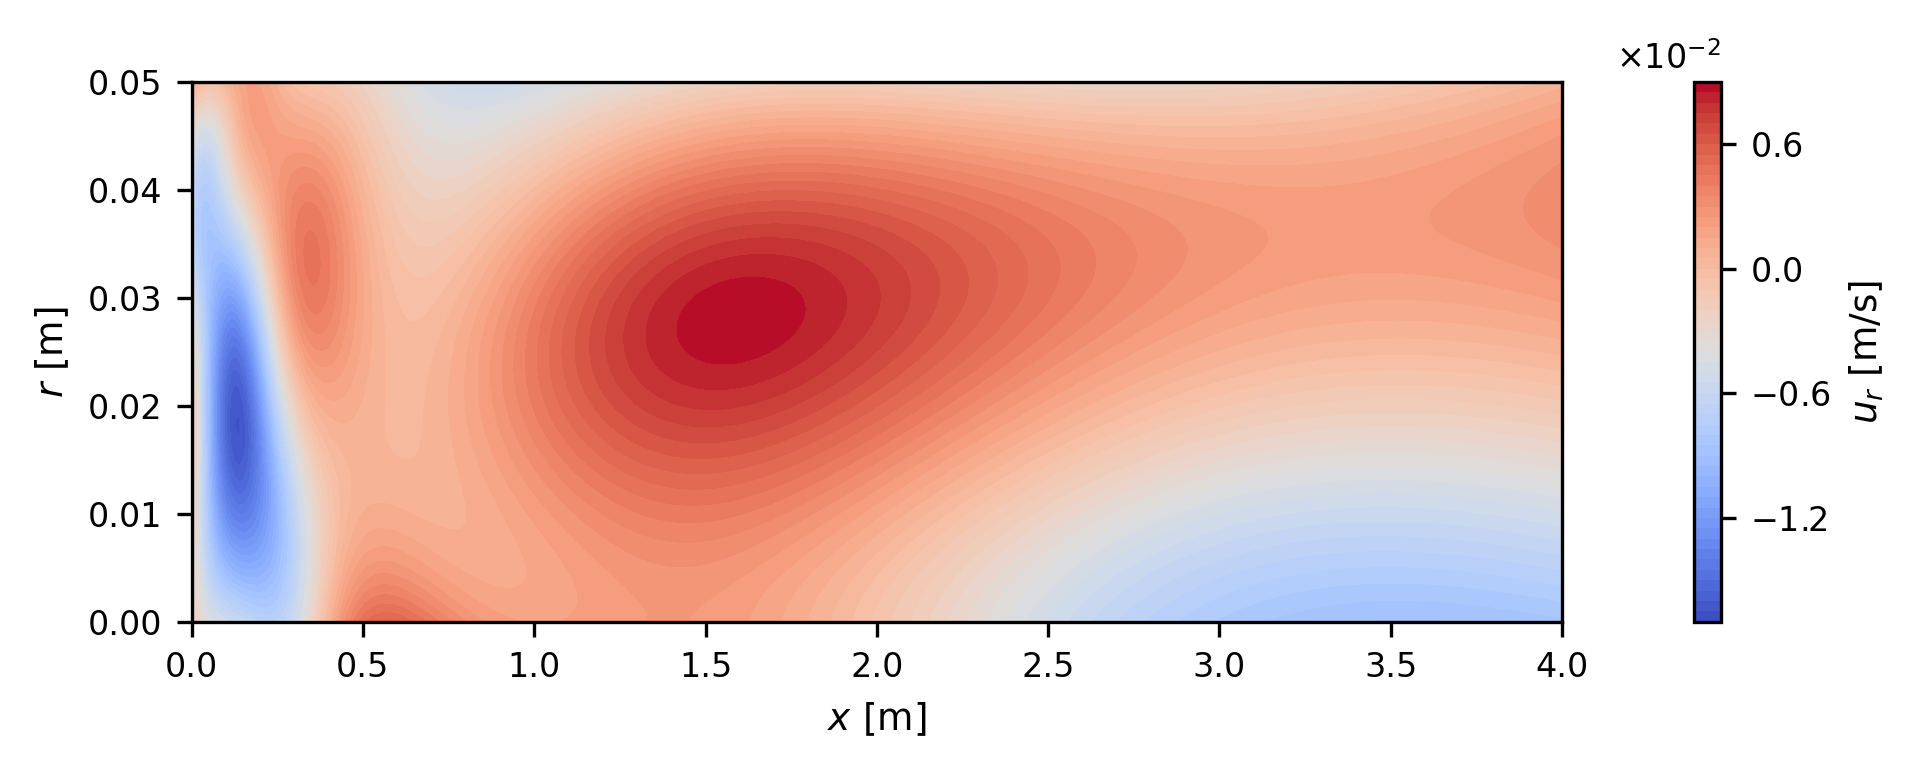
\includegraphics[width=\textwidth]{stage2_pred_ur_Re600.png}
\caption{Radial velocity $u_r$ [m/s].}
\end{subfigure}
\vskip\baselineskip
\begin{subfigure}[b]{0.48\textwidth}
\centering
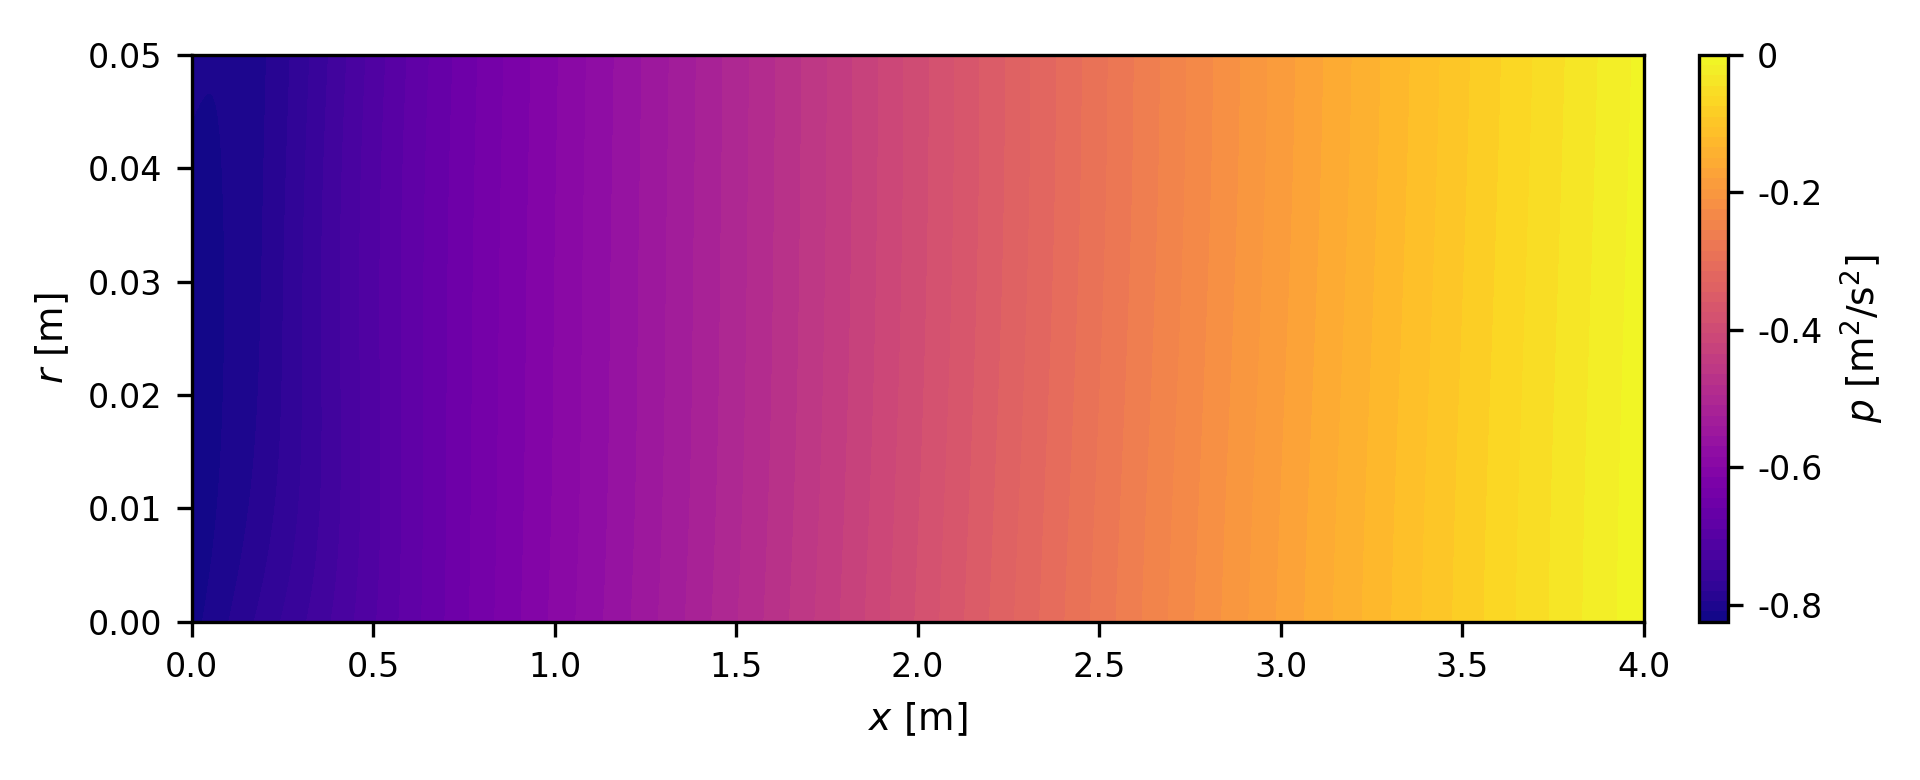
\includegraphics[width=\textwidth]{stage2_pred_p_Re600.png}
\caption{Kinematic pressure $p$ [$\mathrm{m^2/s^2}$].}
\end{subfigure}
\hfill
\begin{subfigure}[b]{0.48\textwidth}
\centering
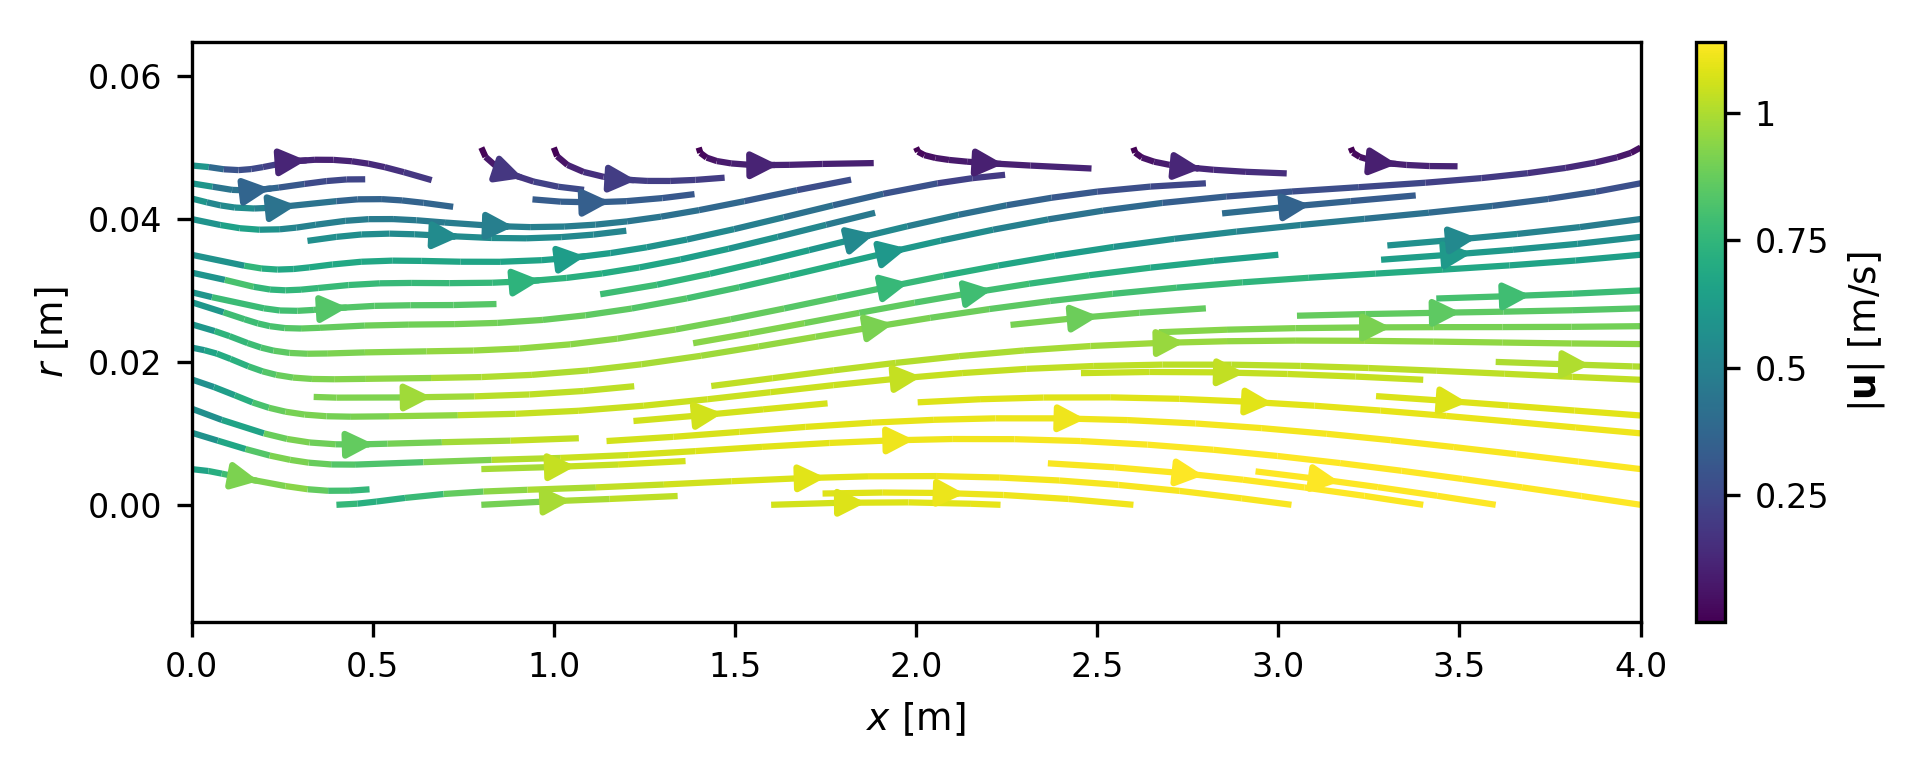
\includegraphics[width=\textwidth]{stage2_pred_streamlines_Re600.png}
\caption{Predicted streamlines colored by speed.}
\end{subfigure}
\caption{Stage 2: Predicted laminar pipe flow fields at $\mathrm{Re} = 600$ (radial axis stretched by a factor $k \approx 29$).}
\label{fig:stage2_pred_re600}
\end{figure}


\subsection{Discussion: Axis Singularity}
The primary challenge in Stage 2 is the $1/r$ geometric coordinate singularity at the centerline. Although L'H\^opital's rule resolves the singularity analytically, automatic differentiation near $r=0$ can experience gradient variance spikes. Enforcing $\partial u/\partial r = 0$ and $v=0$ via soft penalties introduces small residual oscillations along the centerline.

% ==============================================================================
% SECTION 5: STAGE 3
% ==============================================================================
\section{Stage 3: Laminar 3D Rectangular Duct Flow}
\label{sec:stage3}

\subsection{Geometry and Physical Problem Setup}
Stage 3 transitions to genuine three-dimensional laminar entrance flow in a rectangular duct. The cross-section has height $H = 0.10\,\text{m}$ and width $W = 0.20\,\text{m}$, defining an aspect ratio $\mathrm{AR} = W/H = 2.0$. The streamwise domain length is $L = 5.0\,\text{m}$. Hydraulic diameter is $D_h = 4(H W) / [2(H+W)] = 4(0.02) / 0.60 = 0.1333\,\text{m}$. Fluid kinematic viscosity is $\nu = 1.0\times 10^{-4}\,\text{m}^2/\text{s}$.

\begin{figure}[H]
\centering
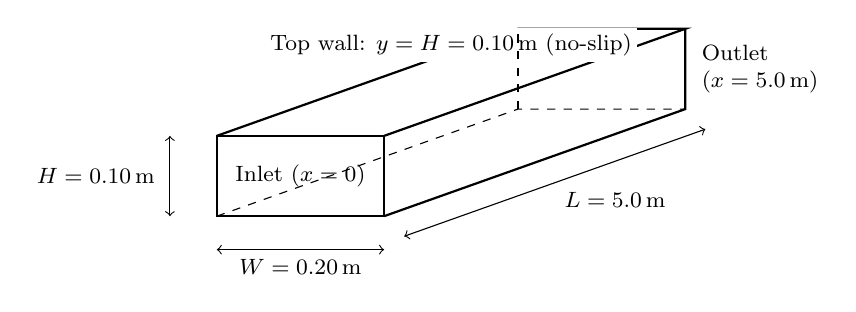
\begin{tikzpicture}[scale=0.85]
    \draw[thick] (0,0) rectangle (2.5, 1.2);
    \node at (1.25, 0.6) [font=\footnotesize, fill=white, inner sep=2pt] {Inlet ($x=0$)};
    \draw[thick] (0,1.2) -- (4.5, 2.8) -- (7.0, 2.8) -- (2.5, 1.2);
    \node[above, font=\footnotesize, fill=white, inner sep=2pt] at (3.5, 2.3) {Top wall: $y = H = 0.10\,\text{m}$ (no-slip)};
    \draw[thick] (2.5,0) -- (7.0, 1.6) -- (7.0, 2.8);
    \draw[dashed] (0,0) -- (4.5, 1.6) -- (7.0, 1.6);
    \draw[dashed] (4.5,1.6) -- (4.5, 2.8);
    \node[right, font=\footnotesize, align=left] at (7.1, 2.2) {Outlet\\($x = 5.0\,\text{m}$)};
    \draw[<->] (0, -0.5) -- (2.5, -0.5) node[midway, below, font=\footnotesize] {$W = 0.20\,\text{m}$};
    \draw[<->] (-0.7, 0) -- (-0.7, 1.2) node[midway, left=2pt, font=\footnotesize] {$H = 0.10\,\text{m}$};
    \draw[<->] (2.8, -0.3) -- (7.3, 1.3) node[midway, below right, font=\footnotesize] {$L = 5.0\,\text{m}$};
\end{tikzpicture}
\caption{Stage 3 geometry: 3D rectangular duct flow ($\mathrm{AR}=2.0, D_h=0.1333\,\text{m}$).}
\label{fig:stage3_geom}
\end{figure}

The Reynolds number is $\mathrm{Re} = U_{\mathrm{mean}} D_h / \nu \implies U_{\mathrm{mean}}(\mathrm{Re}) = 0.00075\,\mathrm{Re}\,\text{m/s}$. At $\mathrm{Re}=100$, mean velocity is $U_{\mathrm{mean}} = 0.075\,\text{m/s}$. Downstream, the flow converges to the analytical Fourier series solution, where the peak centerline velocity reaches $u_{\max}/U_{\mathrm{mean}} = 1.992$ for an $\mathrm{AR}=2.0$ duct.

\subsection{Governing Equations and Dimensionless Formulation}
The steady incompressible 3D Navier--Stokes equations in Cartesian coordinates $(x, y, z)$ are:
\begin{align}
\frac{\partial u}{\partial x} + \frac{\partial v}{\partial y} + \frac{\partial w}{\partial z} &= 0, \\
u \frac{\partial u}{\partial x} + v \frac{\partial u}{\partial y} + w \frac{\partial u}{\partial z} &= -\frac{\partial p}{\partial x} + \nu \nabla^2 u, \\
u \frac{\partial v}{\partial x} + v \frac{\partial v}{\partial y} + w \frac{\partial v}{\partial z} &= -\frac{\partial p}{\partial y} + \nu \nabla^2 v, \\
u \frac{\partial w}{\partial x} + v \frac{\partial w}{\partial y} + w \frac{\partial w}{\partial z} &= -\frac{\partial p}{\partial z} + \nu \nabla^2 w.
\end{align}
No-slip conditions apply at all four walls: $u=v=w=0$ at $y \in \{0, H\}$ and $z \in \{0, W\}$.

\subsection{Reference Marching Solver and Spatial Discretization}
Reference data was computed using an independent 3D parabolized finite-difference marching code (\texttt{3/duct\_solver.py}). The solver drops streamwise diffusion ($\partial^2 u/\partial x^2 = 0$) and cross-stream pressure gradients ($\partial p/\partial y = \partial p/\partial z = 0 \implies p = p(x)$). The computational grid comprises $N_x = 3624$ axial stations, $N_y = 41$ vertical points, and $N_z = 81$ horizontal points ($3624 \times 41 \times 81 = 12{,}035{,}304$ spatial nodes). Mass conservation $\int_0^W \int_0^H u\,dy\,dz = H W U_{\mathrm{mean}}$ is enforced via pressure-gradient superposition at each axial step.

As noted in Section~\ref{sec:elliptic_vs_parabolic}, the network is trained on the full 3D Navier--Stokes equations whereas the reference solver neglects axial diffusion; the resulting difference is largest near the inlet.

\subsection{Network Design and Hyperparameters}
\label{sec:stage3_arch}
% src: 3/pinn_model.py:61,72
The Stage 3 network (\texttt{3/pinn\_model.py}, class \texttt{DuctPINN}) takes four normalized inputs. The Reynolds number embedding $\mathrm{Re}_n$ is normalized over the full evaluation sweep $\mathrm{Re} \in [50, 600]$ ($\mathrm{Re}_{\min}=50, \mathrm{Re}_{\max}=600$, yielding $\mathrm{Re}_n = -0.4421$ at $\mathrm{Re}=100$; code \texttt{3/pinn\_model.py:27}):
\begin{equation}
\label{eq:stage3_renorm}
\hat{x} = \frac{x}{L}, \quad \hat{y} = \frac{y}{H}, \quad \hat{z} = \frac{z}{W}, \quad \mathrm{Re}_n = 2\frac{\log_{10}(\mathrm{Re}) - \log_{10}(50)}{\log_{10}(600) - \log_{10}(50)} - 1 \in [-1, 1].
\end{equation}
The normalization constants are fixed numbers; $\mathrm{Re} = 600$ does not enter the training set (training Reynolds numbers: 50, 100, 200, 500). Because the normalization range includes $\mathrm{Re} = 600$, the $\mathrm{Re} = 600$ test case lies at the edge of the normalized input range ($\mathrm{Re}_n = +1$), not outside it. No $\mathrm{Re} = 600$ data are used in training, so the case is an unseen Reynolds number; it is not an extrapolation in the sense used in Stages~4 and 5, where the test inputs lie outside the normalized training range.
The architecture contains four hidden layers of 80 neurons with $\tanh$ activations ($[4, 80, 80, 80, 80, 4]$, 20,164 parameters). Training uses Adam for 2500 iterations ($8.0\times 10^{-4}$ decayed via StepLR every 500 steps) followed by 300 iterations of L-BFGS polish.
% src: 3/train_hybrid.py:147-148
At each iteration, $N_{\mathrm{data}} = 2{,}000$ data points are sampled from the reference solution, and $N_{\mathrm{pde}} = 4{,}000$ collocation points are drawn uniformly across $[0, L] \times [0, H] \times [0, W]$. Collocation counts are 2,000 data points, 4,000 interior PDE points, and 1,000 boundary points.

\subsection{Composite Loss Formulation and Final Loss Weights}
The composite loss minimizes eight objective terms:
\begin{equation}
\mathcal{L} = w_{u}\mathcal{L}_{u} + w_{v}\mathcal{L}_{v} + w_{w}\mathcal{L}_{w} + w_{p}\mathcal{L}_{p} + w_{\mathrm{pde}}\mathcal{L}_{\mathrm{pde}} + w_{\mathrm{in}}\mathcal{L}_{\mathrm{in}} + w_{\mathrm{wall}}\mathcal{L}_{\mathrm{wall}} + w_{\mathrm{out}}\mathcal{L}_{\mathrm{out}}.
\end{equation}
The final loss weights read directly from \texttt{3/config.py} are:
\begin{equation}
% src: 3/config.py Line 85
\begin{aligned}
w_{u} &= 8.733, \quad & w_{v} &= 0.110, \quad & w_{w} &= 11.109, \quad & w_{p} &= 2.421, \\
w_{\mathrm{pde}} &= 32.183, \quad & w_{\mathrm{in}} &= 0.683, \quad & w_{\mathrm{wall}} &= 11.138, \quad & w_{\mathrm{out}} &= 0.639.
\end{aligned}
\end{equation}

\subsection{Forward Pass at a Single Point}
The pre-activation vector $z = W a_{\mathrm{prev}} + b$ represents the affine combination entering each layer, while the post-activation $a = \tanh(z)$ is its bounded output. Matrix $\|W\|_F$ denotes the Frobenius norm of the layer weight matrix, $\|b\|_2$ is the Euclidean norm of the bias vector, and $z[1:4]$ reports the numerical values of the first four neurons of each layer.

Table~\ref{tab:stage3_act} reports the deterministic forward pass evaluated from \texttt{3/checkpoints/duct\_pinn.pt} at the duct centerline $(x=2.5\,\text{m}, y=0.05\,\text{m}, z=0.10\,\text{m}, \mathrm{Re}=100)$.
\begin{table}[H]
\centering
\resizebox{\linewidth}{!}{%
\begin{tabular}{lcccc}
\toprule
\textbf{Network Layer} & \textbf{Pre-activations} $z_{[1:4]}$ & \textbf{Post-activations} $a_{[1:4]} = \tanh(z)$ & $\|W\|_F$ & $\|b\|_2$ \\
\midrule
Hidden 1 & $[-0.2847, -0.1165, 0.4132, 0.0802]$ & $[-0.2773, -0.1160, 0.3912, 0.0801]$ & 2.93 & 0.65 \\
Hidden 2 & $[-0.1891, 0.2480, -0.0711, 0.0232]$ & $[-0.1869, 0.2430, -0.0710, 0.0232]$ & 9.47 & 0.44 \\
Hidden 3 & $[0.6916, -0.3750, -0.1283, 0.2216]$ & $[0.5990, -0.3584, -0.1276, 0.2181]$ & 9.36 & 0.26 \\
Hidden 4 & $[0.1684, -0.4821, -0.1735, -0.1191]$ & $[0.1668, -0.4479, -0.1717, -0.1185]$ & 9.12 & 0.16 \\
Output & $[2.1008, -0.0022, -0.0020, 0.3058]$ & N/A & 2.96 & 0.04 \\
\bottomrule
\end{tabular}%
}
\caption{Deterministic layer-by-layer forward pass evaluated at $(x=2.5\,\text{m}, y=0.05\,\text{m}, z=0.10\,\text{m}, \mathrm{Re}=100)$. Normalized input vector: $[0.5000, 0.5000, 0.5000, -0.4421]^{\mathsf T}$. Checkpoint SHA256: \texttt{fa39850d5892dc98...}.}
\label{tab:stage3_act}
\end{table}
% src: 3/pinn_model.py:84-85; verify_forward_pass.py
Unlike Stage~1 ($p_{\mathrm{scale}} = 0.5 U_0^2$) and Stage~2 ($p_{\mathrm{scale}} = 32\nu U_0 L / D^2$), the Stage~3 scale $p_{\mathrm{scale}} = 0.5 U_{\mathrm{ref}}^2 (L / D_h) = 0.10547\,\text{m}^2/\text{s}^2$ scales dynamic pressure by duct slenderness $L / D_h = 37.5$ to characterize cumulative frictional pressure drop. The normalized inputs evaluate to $\hat{x}=0.5$, $\hat{y}=0.5$, $\hat{z}=0.5$, and $\mathrm{Re}_n=-0.4421$. With $U_{\mathrm{ref}} = 0.075$ m/s and $p_{\mathrm{scale}} = 0.10547$ m$^2$/s$^2$, physical predictions are:
\begin{align}
% src: 3/checkpoints/duct_pinn.pt; verify_forward_pass.py
u &= 2.1008 \times 0.075 = \mathbf{0.15756\,\text{m/s}} \quad (\text{reference: } 0.14947\,\text{m/s}, \text{ error } 5.41\%), \\
v &= -0.0022 \times 0.075 = -0.000165\,\text{m/s}, \\
w &= -0.0020 \times 0.075 = -0.000150\,\text{m/s}, \\
p &= 0.3058 \times 0.10547 = \mathbf{0.03226\,\text{m}^2/\text{s}^2} \quad (\text{reference gauge: } 0.03267\,\text{m}^2/\text{s}^2, \text{ error } 1.27\%).
\end{align}
At mid-domain ($x=2.5\,\text{m}$), the predicted centerline velocity ratio is $u/U_{\mathrm{mean}} = 2.1008$ ($+5.46\%$ above the fully developed value of $1.992$).

\subsection{Empirical Results and Centerline Velocity Profiles}
Table~\ref{tab:stage3_metrics} compiles quantitative errors across all evaluated Reynolds numbers. These $L_2$ errors include the reference inlet transient and the outlet gauge offset; they do not measure the friction gradient alone. For the developed region $x \in [1.5, 5.0]\,\text{m}$ the comparison of pressure gradients is given in Table~\ref{tab:stage3_dp_ratio} (slope ratios $0.22$ to $1.04$); the full-domain $L_2$ error is dominated by the inlet transient and the gauge difference.
\begin{table}[H]
\centering
\resizebox{\textwidth}{!}{
\begin{tabular}{lcccccc}
\toprule
\textbf{Metric Variable} & $\mathbf{Re=50}$ & $\mathbf{Re=100}$ & $\mathbf{Re=200}$ & $\mathbf{Re=300}$ (TEST-interp) & $\mathbf{Re=500}$ & $\mathbf{Re=600}$ (TEST-extrap) \\
\midrule
$u$ (Axial Velocity Rel $L_2$) & 8.81\% & 8.91\% & 9.77\% & 10.62\% & 12.08\% & 12.69\% \\
$v$ (Vertical Velocity Rel $L_2$) & 2.79\% & 2.46\% & 2.02\% & 1.74\% & 1.40\% & 1.30\% \\
$w$ (Horizontal Velocity Rel $L_2$) & 1.72\% & 1.42\% & 1.11\% & 0.94\% & 0.73\% & 0.66\% \\
$p$ (Kinematic Pressure Rel $L_2$) & 80.70\% & 73.86\% & 66.66\% & 56.77\% & 67.22\% & 106.39\% \\
\bottomrule
\end{tabular}
}
\caption{Stage 3: Full-domain relative $L_2$ errors for 3D rectangular duct flow (Source: \texttt{3/figures/global\_summary.txt}).}
\label{tab:stage3_metrics}
\end{table}


Centerline velocity evaluation at the duct exit ($x=5.0\,\text{m}, y=0.05\,\text{m}, z=0.10\,\text{m}$) directly evaluated from checkpoint \texttt{3/checkpoints/duct\_pinn.pt} yields:
\begin{itemize}[leftmargin=1.5em]
    \item $\mathrm{Re}=100$: Exit velocity $u_{\mathrm{exit}} = 0.16160\,\text{m/s} \implies u_{\mathrm{exit}}/U_{\mathrm{mean}} = \mathbf{2.1547}$ ($+8.17\%$ overprediction vs.\ analytical series $1.992$).
    \item $\mathrm{Re}=300$: Exit velocity $u_{\mathrm{exit}} = 0.47149\,\text{m/s} \implies u_{\mathrm{exit}}/U_{\mathrm{mean}} = \mathbf{2.0955}$ ($+5.20\%$ overprediction vs.\ analytical series $1.992$).
\end{itemize}


\subsection{Predicted Flow Fields}
Figures~\ref{fig:stage3_pred_crossplanes_re100} through~\ref{fig:stage3_pred_longitudinal} illustrate the predicted three-dimensional laminar duct flow fields ($H=0.10\,\text{m}$, $W=0.20\,\text{m}$, $L=5.0\,\text{m}$) at $\mathrm{Re} = 100$ and $600$.

Predicted cross-plane velocities ($u, v, w$) at $x = 1.0\,\text{m}$ and $x = 5.0\,\text{m}$ illustrate the two-dimensional boundary-layer growth originating from the rectangular conduit perimeter. Mid-plane contours ($z = W/2$) capture the progressive acceleration of the duct core velocity towards its fully developed peak. The centerline pressure profiles exhibit a continuous axial drop along the conduit length.

\begin{figure}[H]
\centering
\begin{subfigure}[b]{0.32\textwidth}
\centering
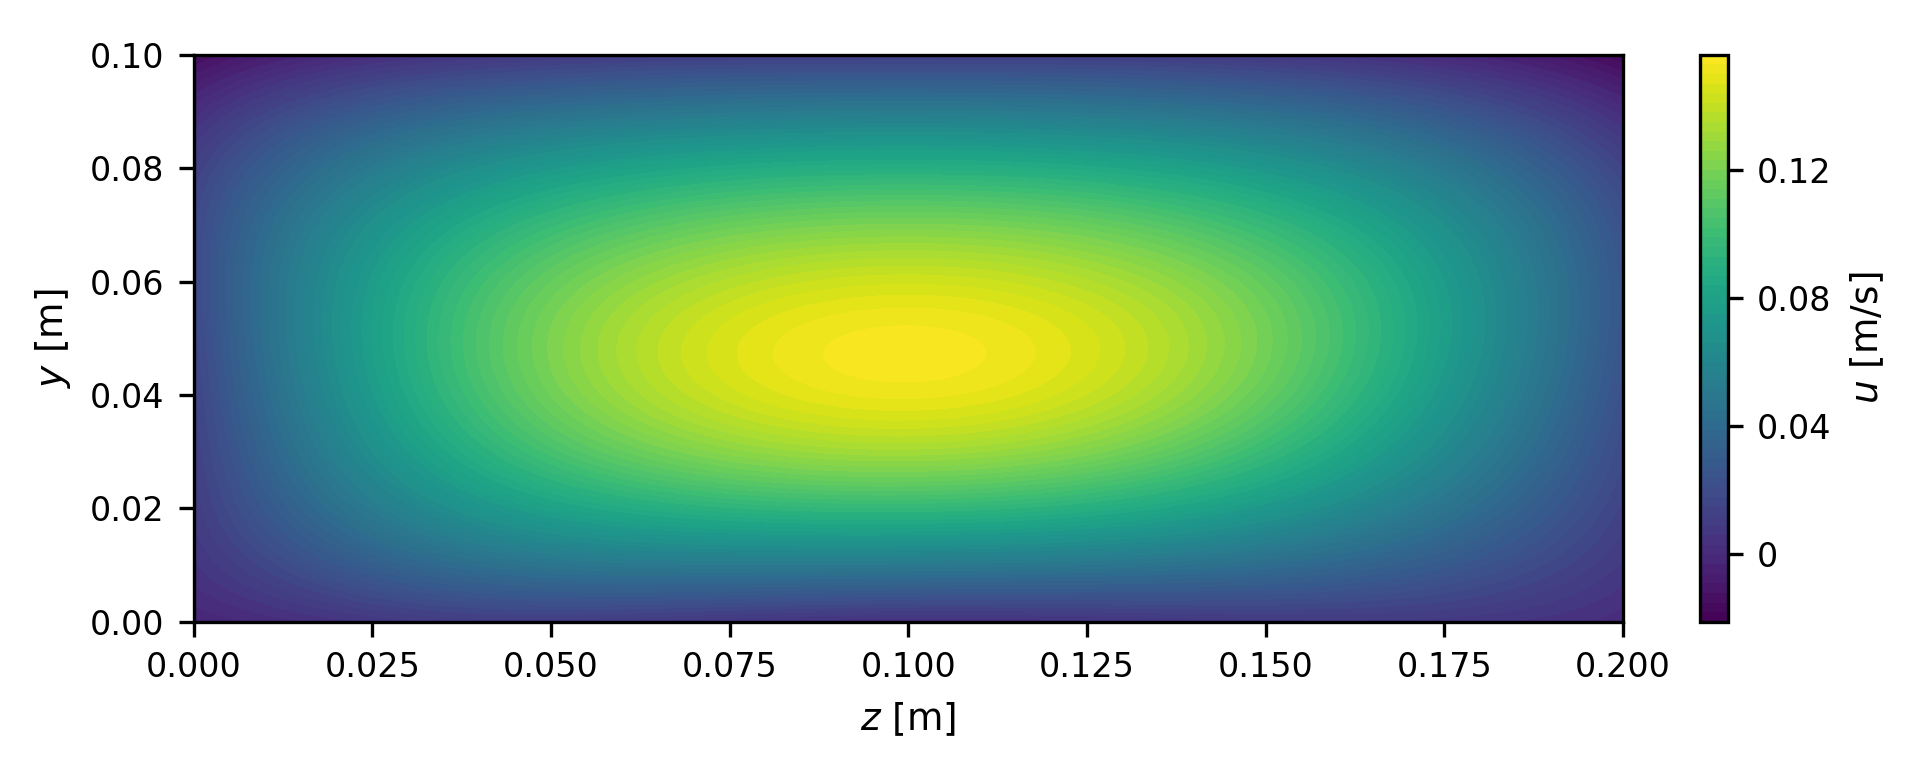
\includegraphics[width=\textwidth]{stage3_pred_u_x1m_Re100.png}
\caption{$u$ at $x=1.0\,\text{m}$ [m/s].}
\end{subfigure}
\hfill
\begin{subfigure}[b]{0.32\textwidth}
\centering
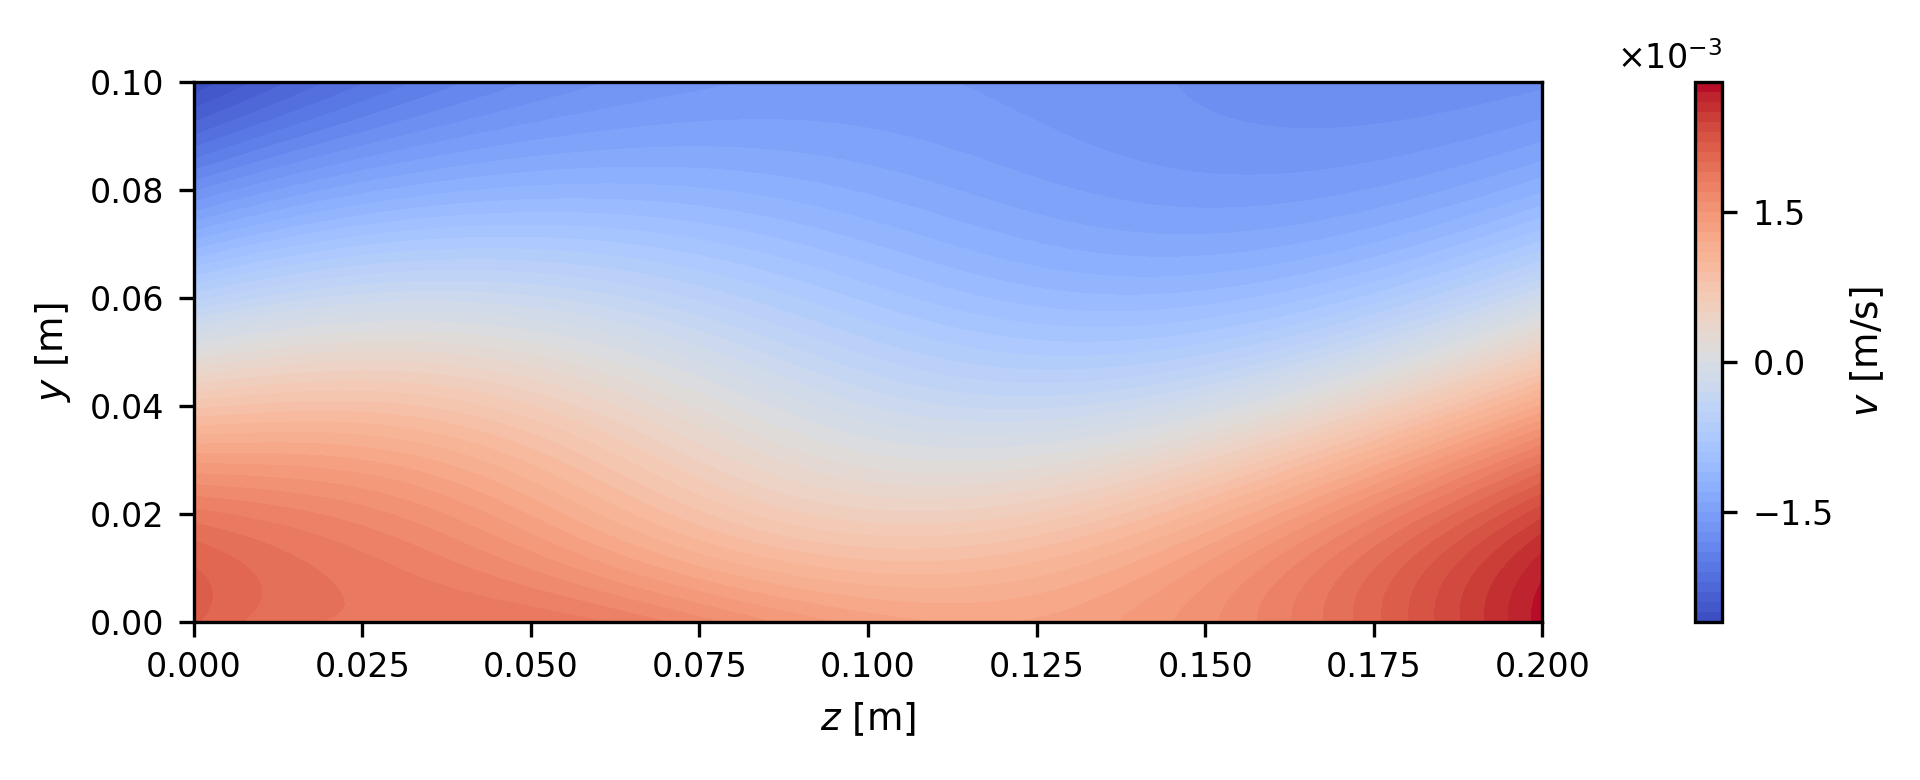
\includegraphics[width=\textwidth]{stage3_pred_v_x1m_Re100.png}
\caption{$v$ at $x=1.0\,\text{m}$ [m/s].}
\end{subfigure}
\hfill
\begin{subfigure}[b]{0.32\textwidth}
\centering
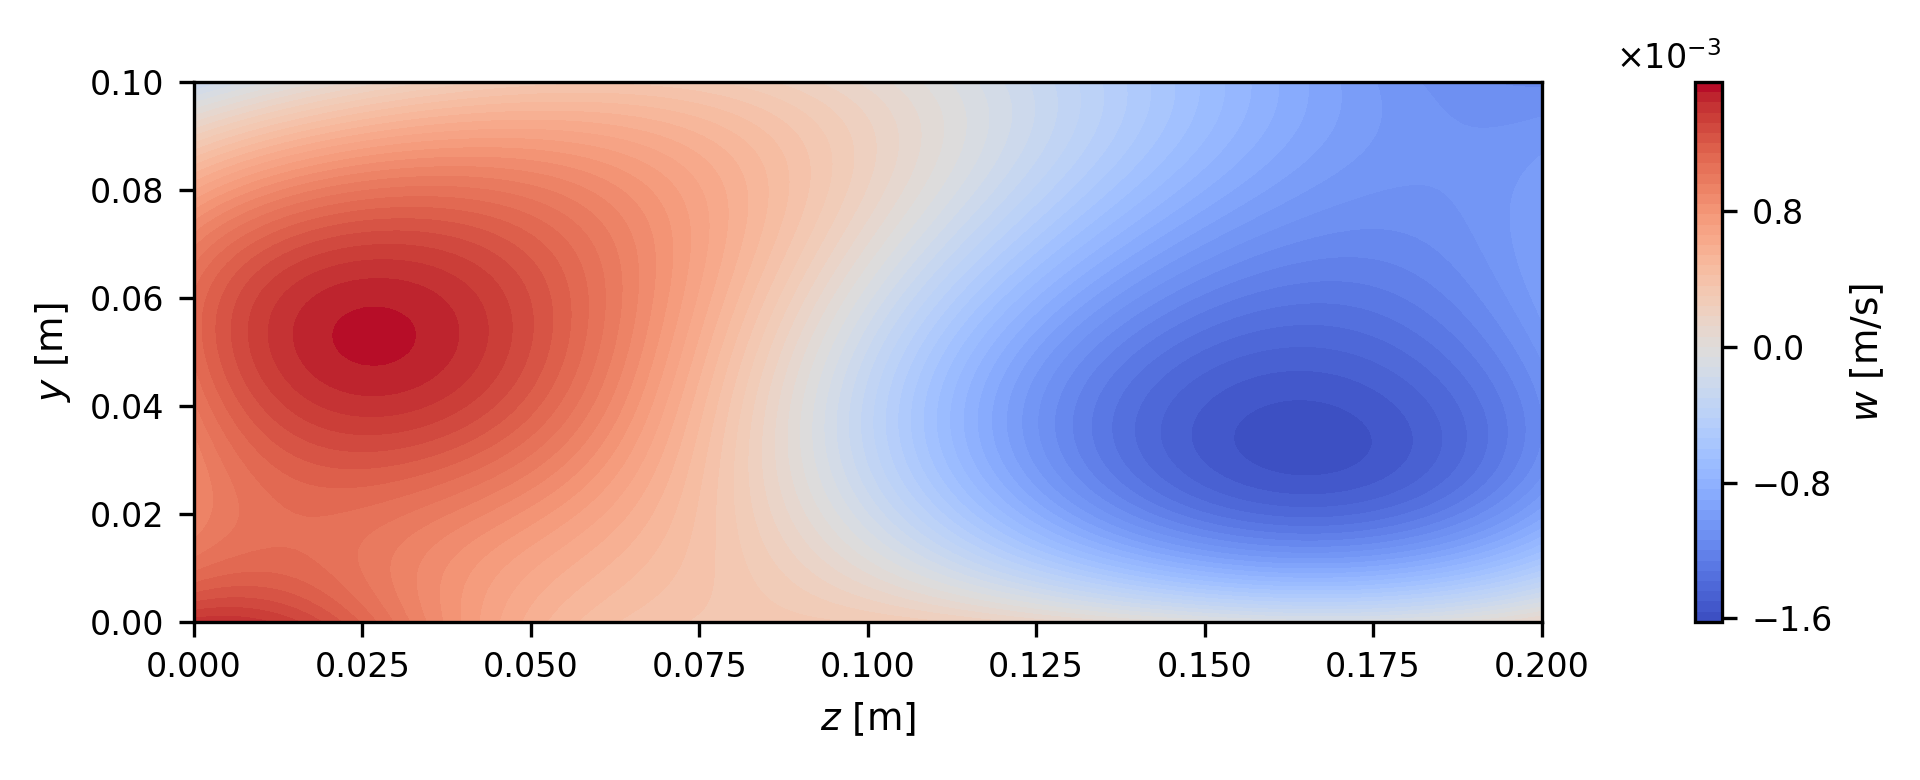
\includegraphics[width=\textwidth]{stage3_pred_w_x1m_Re100.png}
\caption{$w$ at $x=1.0\,\text{m}$ [m/s].}
\end{subfigure}
\vskip\baselineskip
\begin{subfigure}[b]{0.32\textwidth}
\centering
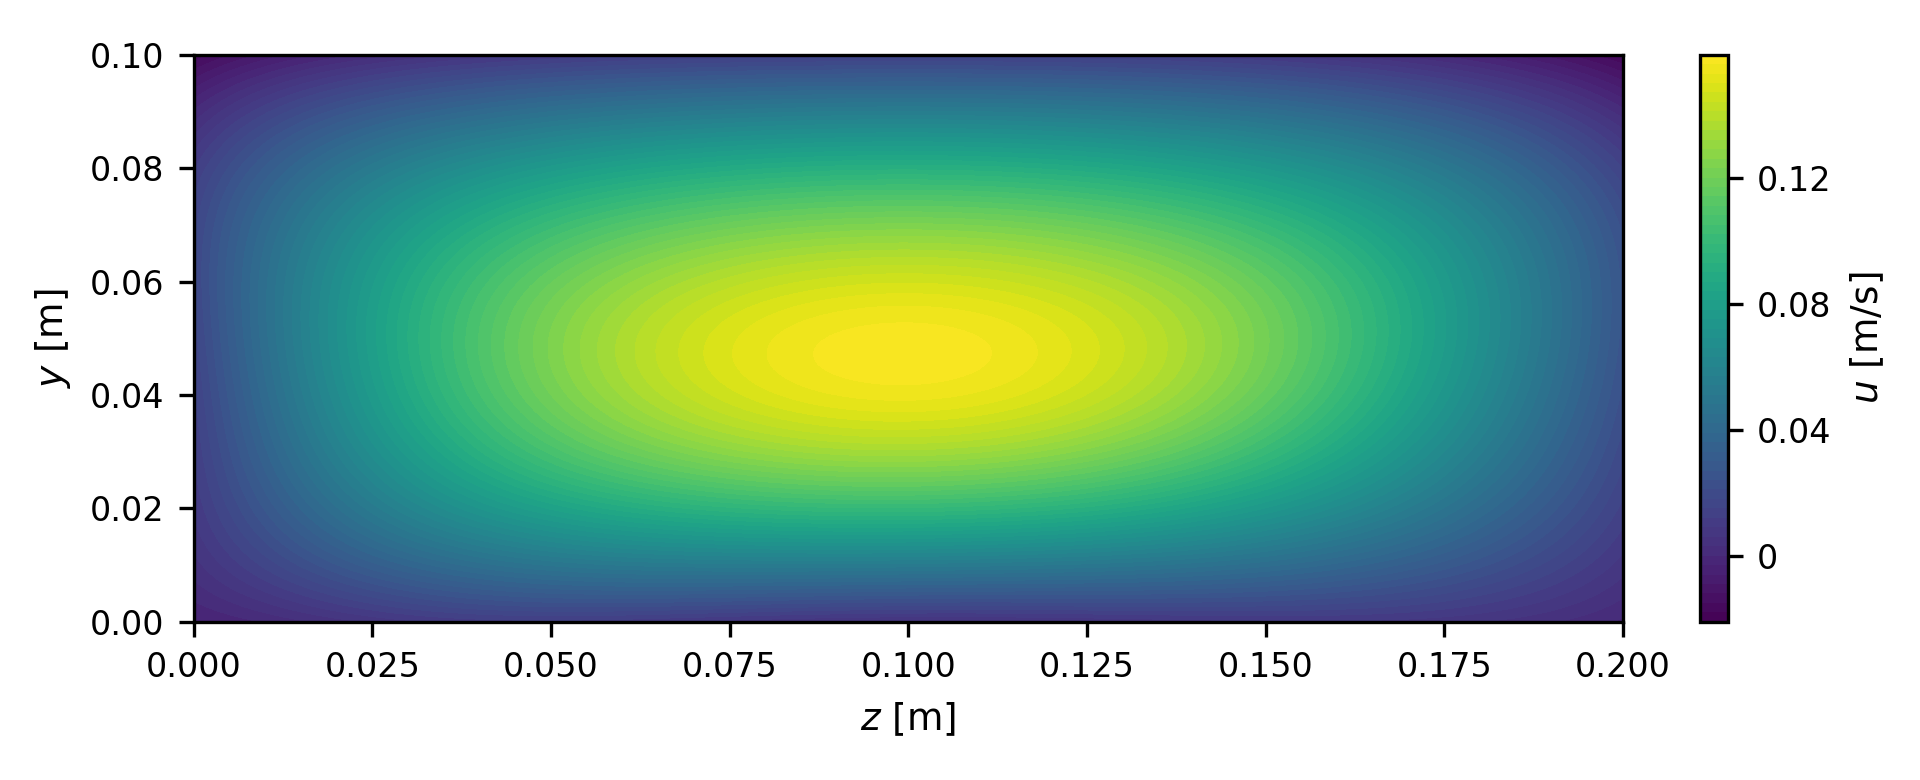
\includegraphics[width=\textwidth]{stage3_pred_u_x5m_Re100.png}
\caption{$u$ at $x=5.0\,\text{m}$ [m/s].}
\end{subfigure}
\hfill
\begin{subfigure}[b]{0.32\textwidth}
\centering
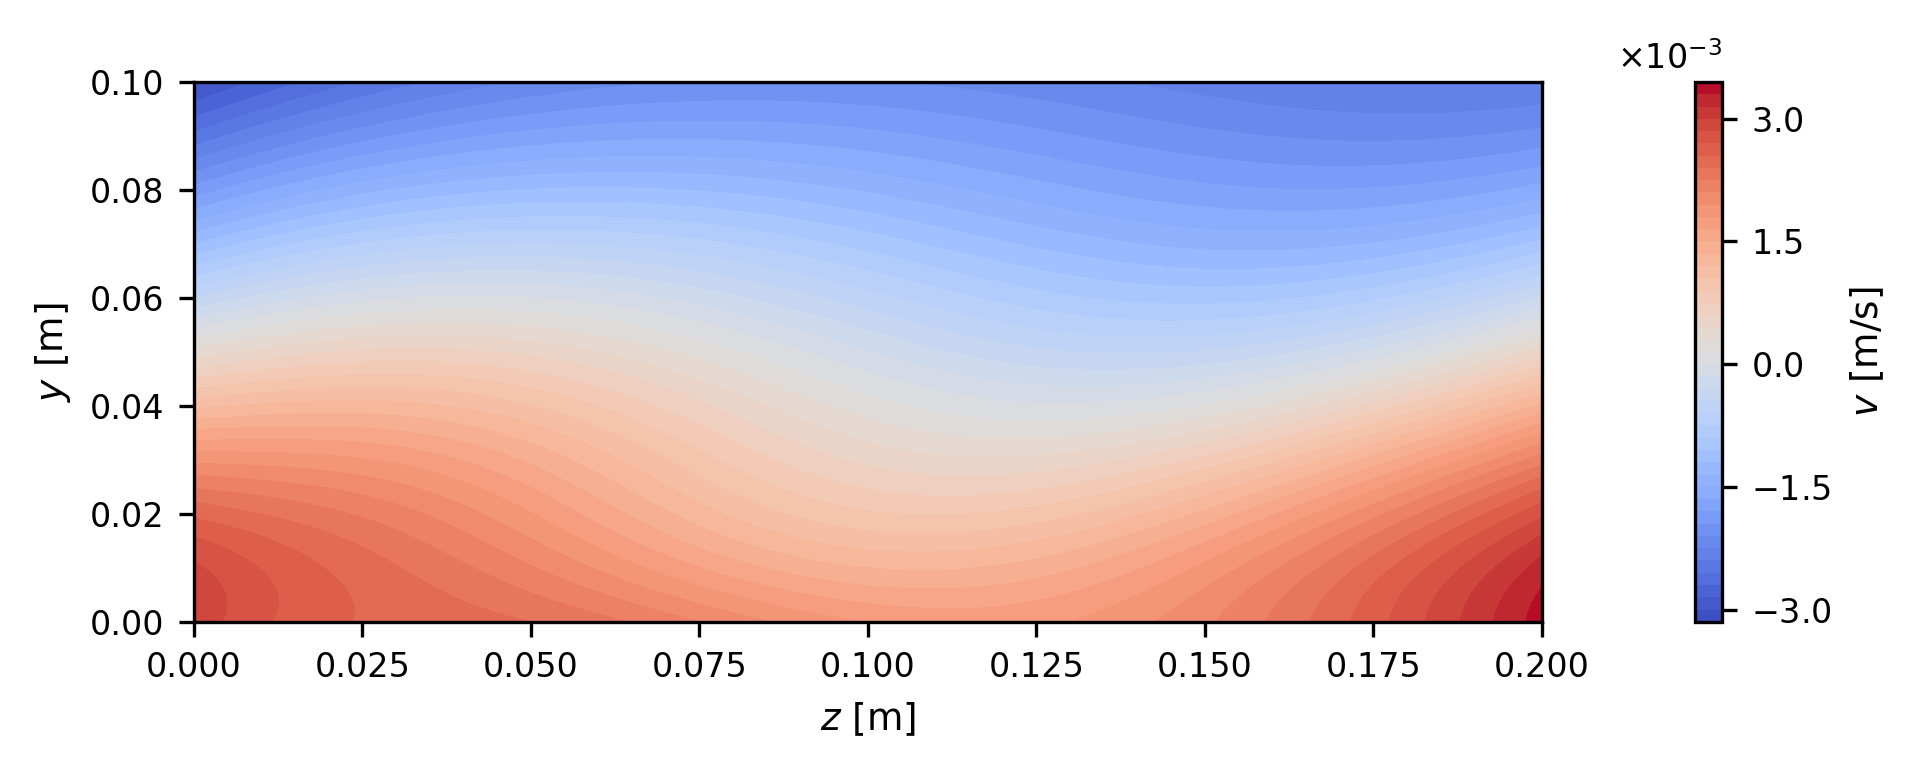
\includegraphics[width=\textwidth]{stage3_pred_v_x5m_Re100.png}
\caption{$v$ at $x=5.0\,\text{m}$ [m/s].}
\end{subfigure}
\hfill
\begin{subfigure}[b]{0.32\textwidth}
\centering
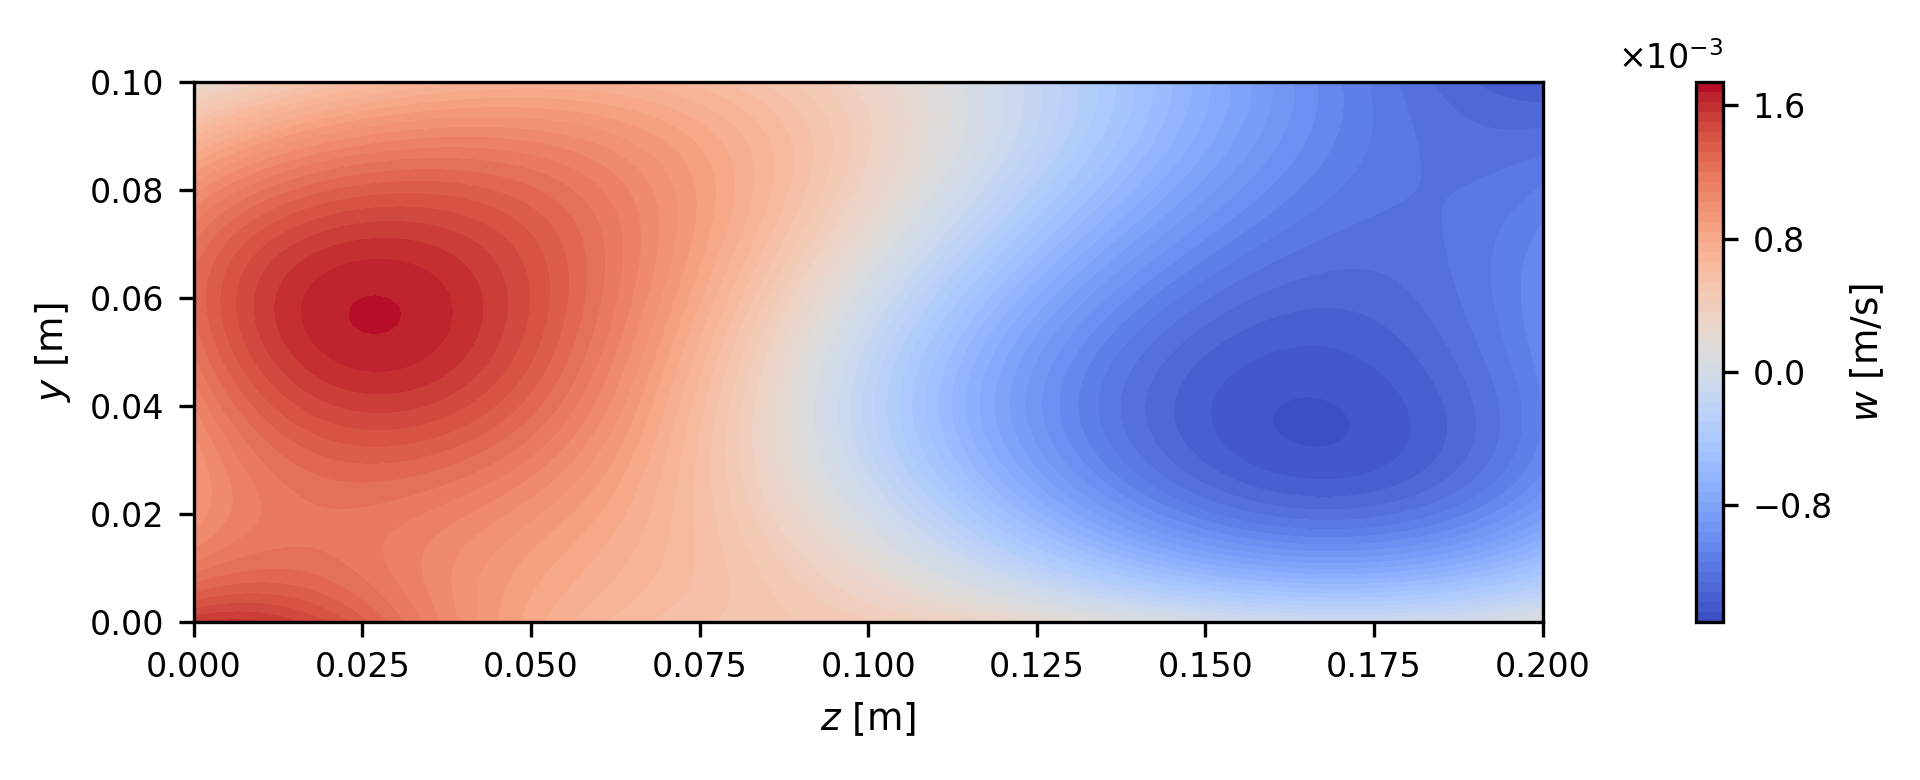
\includegraphics[width=\textwidth]{stage3_pred_w_x5m_Re100.png}
\caption{$w$ at $x=5.0\,\text{m}$ [m/s].}
\end{subfigure}
\caption{Stage 3: Predicted cross-plane velocity fields ($u, v, w$) at $x = 1.0\,\text{m}$ and $x = 5.0\,\text{m}$ for $\mathrm{Re} = 100$.}
\label{fig:stage3_pred_crossplanes_re100}
\end{figure}

\begin{figure}[H]
\centering
\begin{subfigure}[b]{0.48\textwidth}
\centering
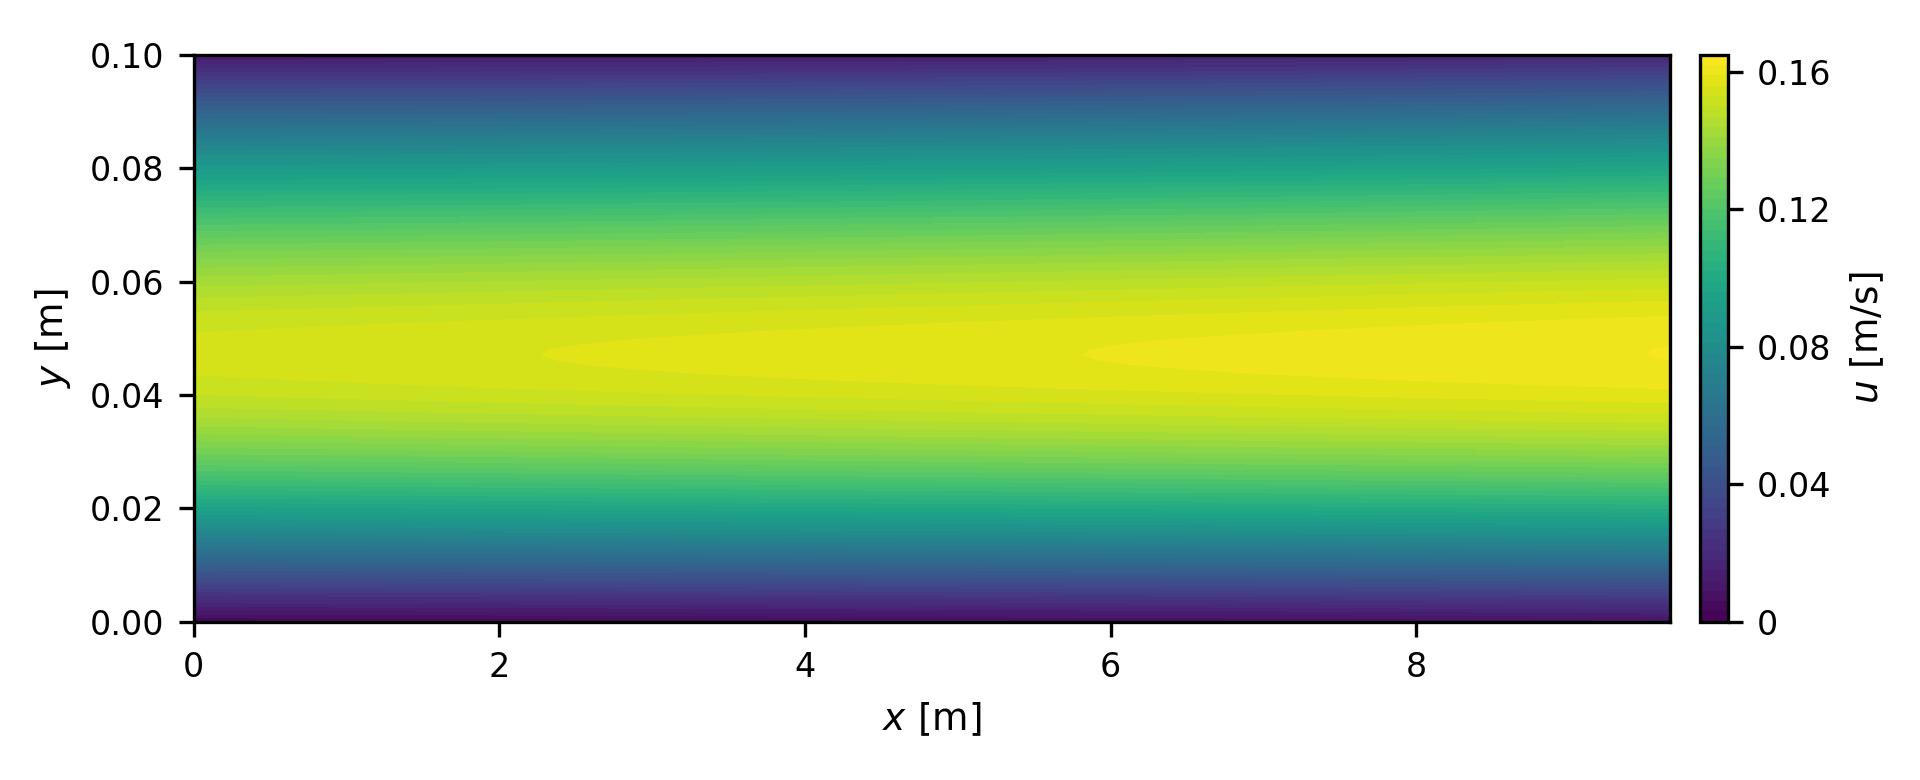
\includegraphics[width=\textwidth]{stage3_pred_u_midplane_Re100.png}
\caption{Mid-plane axial velocity $u$ ($z = W/2$) [m/s].}
\end{subfigure}
\hfill
\begin{subfigure}[b]{0.48\textwidth}
\centering
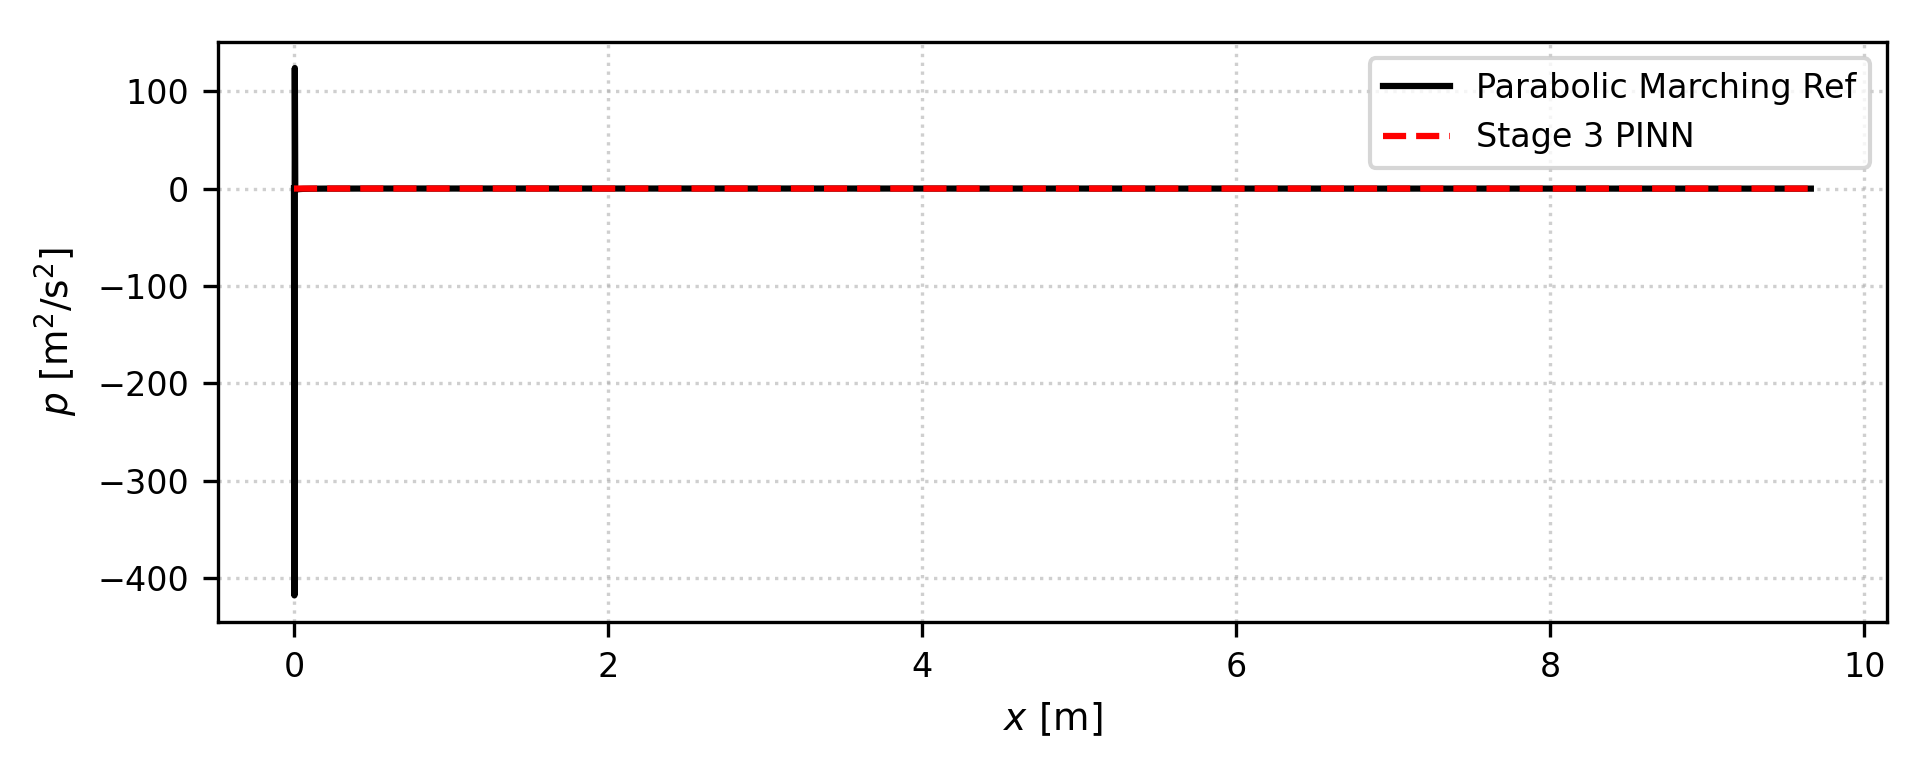
\includegraphics[width=\textwidth]{stage3_pred_p_centerline_Re100.png}
\caption{Centerline kinematic pressure $p(x)$ [$\mathrm{m^2/s^2}$].}
\end{subfigure}
\vskip\baselineskip
\begin{subfigure}[b]{0.48\textwidth}
\centering
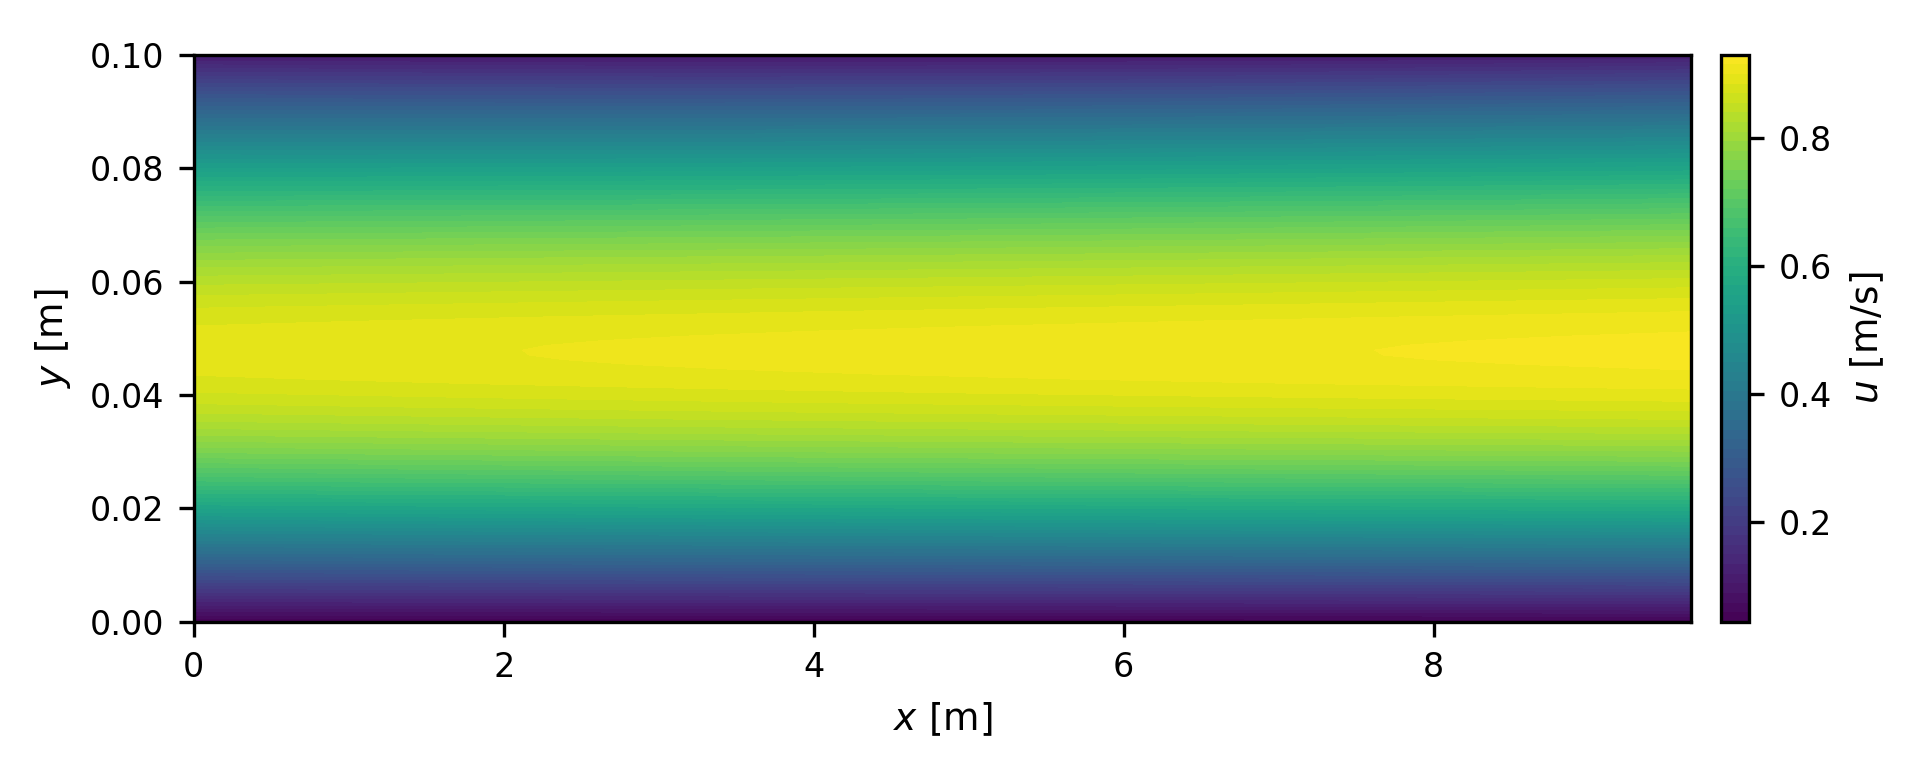
\includegraphics[width=\textwidth]{stage3_pred_u_midplane_Re600.png}
\caption{Mid-plane axial velocity $u$, $\mathrm{Re} = 600$ [m/s].}
\end{subfigure}
\hfill
\begin{subfigure}[b]{0.48\textwidth}
\centering
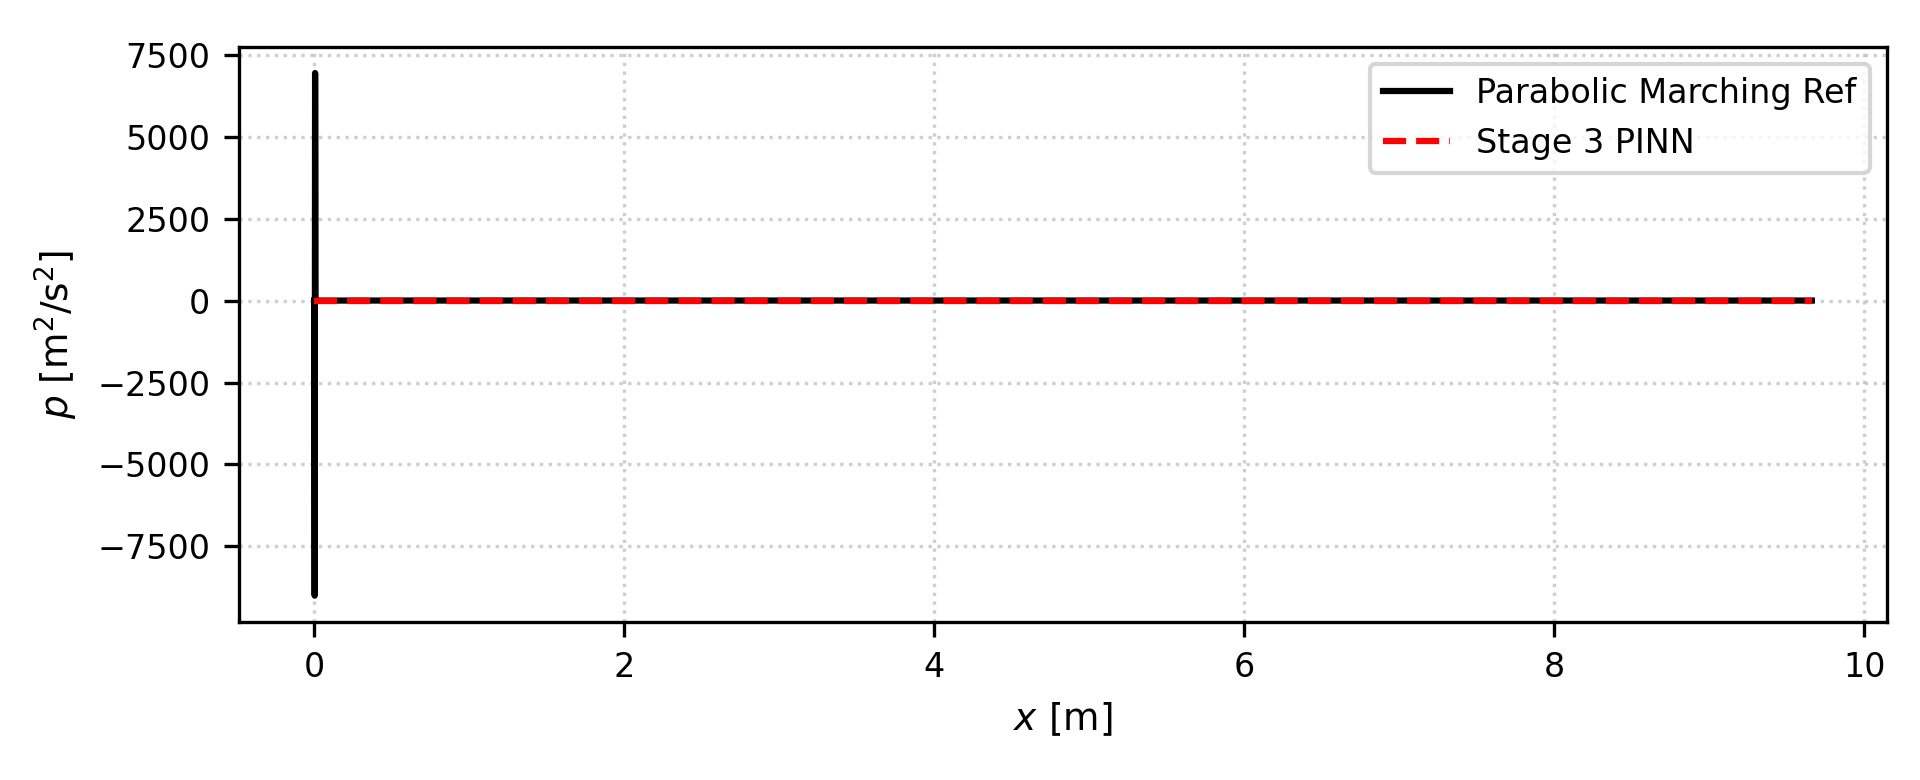
\includegraphics[width=\textwidth]{stage3_pred_p_centerline_Re600.png}
\caption{Centerline kinematic pressure $p(x)$, $\mathrm{Re} = 600$ [$\mathrm{m^2/s^2}$].}
\end{subfigure}
\caption{Stage 3: Longitudinal mid-plane velocity and centerline pressure drop predicted by the PINN at $\mathrm{Re} = 100$ and $600$.}
\label{fig:stage3_pred_longitudinal}
\end{figure}


\subsection{Discussion: Pressure Gradient and Inlet Velocity Error}
Comparative evaluation identifies two primary failure modes in Stage 3:
\begin{enumerate}[leftmargin=1.5em]
% % src: 3/figures/global_summary.txt: $\mathrm{Re}=50: 80.7\%, \mathrm{Re}=100: 73.9\%, \mathrm{Re}=200: 66.7\%, \mathrm{Re}=300: 56.8\%, \mathrm{Re}=500: 67.2\%, \mathrm{Re}=600: 106.4\%$
    \item \textbf{Centerline Pressure Gradient and Inlet Transient Mismatch:} As documented in Table~\ref{tab:stage3_metrics}, kinematic pressure exhibits large relative $L_2$ errors ranging from $\mathbf{56.8\%}$ to $\mathbf{106.4\%}$. In the downstream window ($x \in [1.5, 5.0]\,\text{m}$), both reference solver and PINN predict falling pressure downstream; the PINN pressure slope divided by the reference slope is $0.22$ at $\mathrm{Re}=50$, $0.38$ at $\mathrm{Re}=100$, $0.64$ at $\mathrm{Re}=200$, $0.83$ at $\mathrm{Re}=300$, and $1.01$--$1.04$ at $\mathrm{Re}=500$--$600$ (Table~\ref{tab:stage3_dp_ratio}). Over the full domain $[0.05, 5.0]\,\text{m}$, the reference centerline pressure difference is dominated by an inlet transient ($x < 0.5\,\text{m}$), where $p_{\mathrm{ref}}$ dips to $-0.301\,\mathrm{m^2/s^2}$ at $x=0.05\,\text{m}$ before recovering, producing an apparent full-domain pressure rise ($+0.362\,\mathrm{m^2/s^2}$ at $\mathrm{Re}=100$, $5.5\times$ the analytic fully developed estimate $0.065\,\mathrm{m^2/s^2}$; Fig.~\ref{fig:stage3_centerline_p_analytic}), whereas the PINN pressure falls monotonically ($\Delta p_{\mathrm{PINN}} = -0.022\,\mathrm{m^2/s^2}$). Untested candidate causes include the gauge level (outlet) differing between reference and PINN, different pressure references or gauge conventions between the parabolic reference solver and the full Navier--Stokes network, the modest pressure loss weight ($w_p = 2.421$), and the large pressure scale $p_{\mathrm{scale}}$.
% src: 3/data/duct_Re*.npz; 3/checkpoints/duct_pinn.pt
    \item \textbf{Inlet Centerline Velocity Error:} Examination of Figure~\ref{fig:stage3_errors}a demonstrates that the largest axial velocity errors occur at the \textit{inlet core} ($x < 0.5\,\text{m}$, where local P99 errors reach $26\%$--$68\%$), rather than at the duct corners. This is the region where the flat inlet profile changes fastest; the cause of the larger error was not isolated.
\end{enumerate}

\begin{figure}[H]
\centering
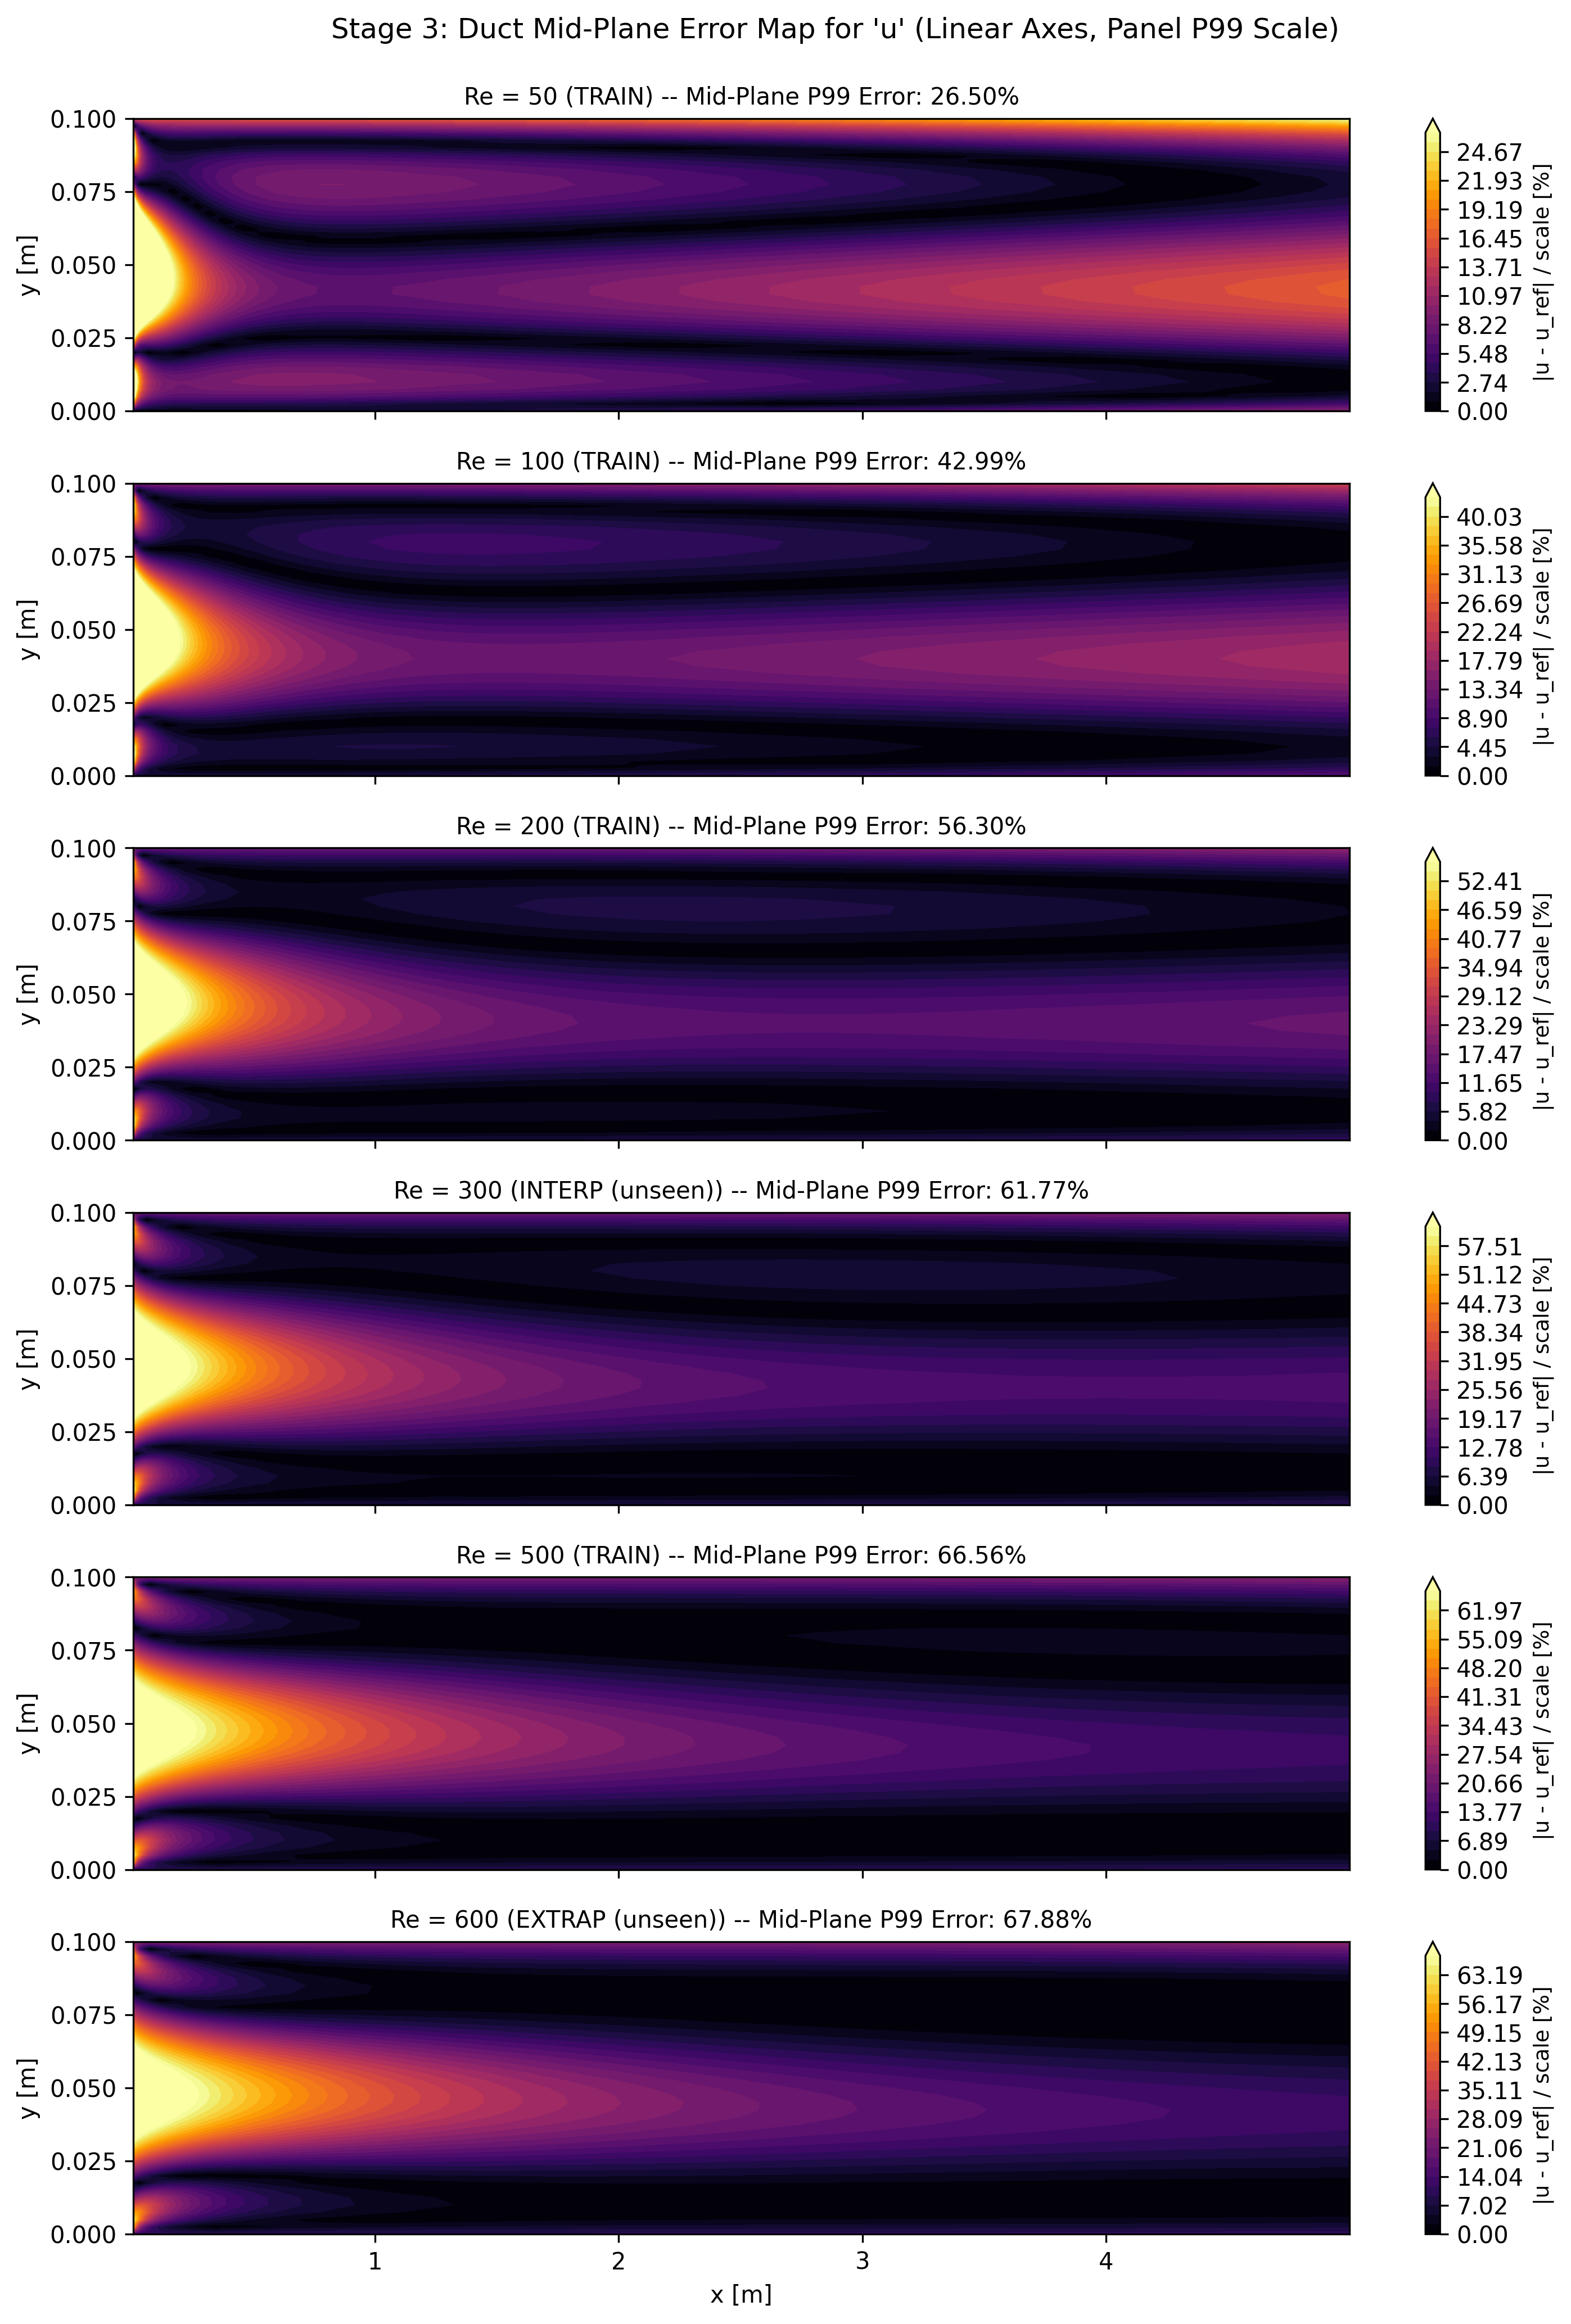
\includegraphics[width=0.92\textwidth]{duct_error_domain_u_linear.png}
\caption{Stage 3: Whole-domain axial velocity error maps for rectangular duct flow ($AR=2.0$).}
\label{fig:stage3_errors}
\end{figure}

% ==============================================================================
% SECTION 6: STAGE 4
% ==============================================================================
\section{Stage 4: Developing Turbulent Channel Flow (RANS + SA)}
\label{sec:stage4}

\subsection{Geometry and Physical Problem Setup}
Stage 4 extends the pipeline to high-Reynolds-number wall-bounded turbulence in a two-dimensional channel ($L/h = 160, \mathrm{Re} \in [10^4, 1.2\times 10^5]$). Due to mid-plane symmetry, the computational domain models the lower half-channel: $x \in [0, 160h]$ and $y \in [0, h]$, where $h = 1.0$ is the half-height.

\begin{figure}[H]
\centering
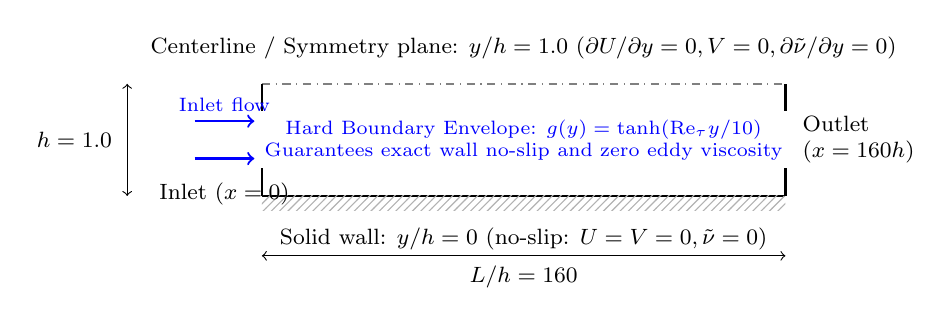
\begin{tikzpicture}[scale=0.95]
    \node[above, font=\footnotesize] at (3.5, 1.7) {Centerline / Symmetry plane: $y/h = 1.0$ ($\partial U/\partial y = 0, V = 0, \partial \tilde{\nu}/\partial y = 0$)};
    \draw[dashdotted, thick, gray] (0, 1.5) -- (7.0, 1.5);
    \draw[thick] (0, 0) -- (7.0, 0);
    \fill[pattern=north east lines, pattern color=gray!60] (0, -0.2) rectangle (7.0, 0);
    \node[below, font=\footnotesize] at (3.5, -0.3) {Solid wall: $y/h = 0$ (no-slip: $U=V=0, \tilde{\nu}=0$)};
    \draw[thick] (0, 0) -- (0, 1.5);
    \draw[blue, thick, ->] (-0.9, 1.0) -- (-0.1, 1.0);
    \draw[blue, thick, ->] (-0.9, 0.5) -- (-0.1, 0.5);
    \node[blue, font=\scriptsize, above] at (-0.5, 1.0) {Inlet flow};
    \node[font=\footnotesize, below] at (-0.5, 0.3) {Inlet ($x=0$)};
    \draw[thick] (7.0, 0) -- (7.0, 1.5);
    \node[right, font=\footnotesize, align=left] at (7.1, 0.75) {Outlet\\($x=160h$)};
    \node[blue, font=\scriptsize, fill=white, inner sep=3pt, align=center] at (3.5, 0.75) {Hard Boundary Envelope: $g(y) = \tanh(\mathrm{Re}_\tau y / 10)$\\Guarantees exact wall no-slip and zero eddy viscosity};
    \draw[<->] (0, -0.8) -- (7.0, -0.8) node[midway, below, font=\footnotesize] {$L/h = 160$};
    \draw[<->] (-1.8, 0) -- (-1.8, 1.5) node[midway, left=2pt, font=\footnotesize] {$h = 1.0$};
\end{tikzpicture}
\caption{Stage 4 geometry: turbulent developing semi-channel domain ($y/h \in [0, 1.0]$).}
\label{fig:stage4_geom}
\end{figure}

Non-dimensionalization sets channel half-height $h = 1.0$ and bulk velocity $U_b = 1.0$. The kinematic viscosity is $\nu = 4/\mathrm{Re}$. The Reynolds number range is parameterized via $\mathrm{Re} = 4\,\mathrm{Re}_h \in [10^4, 1.2\times 10^5]$ (training: $\{10^4, 2\times 10^4, 4\times 10^4, 8\times 10^4\}$; test interpolation: $2.8\times 10^4$; test extrapolation: $9.6\times 10^4, 1.2\times 10^5$).

\subsection{Governing Equations and Spalart--Allmaras RANS Closure}
The flow is governed by the steady 2D Reynolds-Averaged Navier--Stokes equations closed with the one-equation Spalart--Allmaras (SA) model~\cite[Sec.~2.1, p.~2]{allmaras2012}:
\begin{align}
\label{eq:stage4_cont}
\frac{\partial U}{\partial x} + \frac{\partial V}{\partial y} &= 0, \\
\label{eq:stage4_mom_x}
U \frac{\partial U}{\partial x} + V \frac{\partial U}{\partial y} &= -\frac{\partial P}{\partial x} + \frac{\partial}{\partial x}\left(2\nu_{\mathrm{eff}}\frac{\partial U}{\partial x}\right) + \frac{\partial}{\partial y}\left(\nu_{\mathrm{eff}}\left(\frac{\partial U}{\partial y} + \frac{\partial V}{\partial x}\right)\right), \\
\label{eq:stage4_mom_y}
U \frac{\partial V}{\partial x} + V \frac{\partial V}{\partial y} &= -\frac{\partial P}{\partial y} + \frac{\partial}{\partial x}\left(\nu_{\mathrm{eff}}\left(\frac{\partial U}{\partial y} + \frac{\partial V}{\partial x}\right)\right) + \frac{\partial}{\partial y}\left(2\nu_{\mathrm{eff}}\frac{\partial V}{\partial y}\right),
\end{align}
where effective viscosity is $\nu_{\mathrm{eff}} = \nu + \nu_t$, and turbulent eddy viscosity is $\nu_t = \tilde{\nu} f_{v1}$.
The working variable $\tilde{\nu}$ satisfies the transport equation:
\begin{equation}
\label{eq:stage4_sa}
U \frac{\partial \tilde{\nu}}{\partial x} + V \frac{\partial \tilde{\nu}}{\partial y} = c_{b1} \tilde{S} \tilde{\nu} - c_{w1} f_w \left(\frac{\tilde{\nu}}{d}\right)^2 + \frac{1}{\sigma}\left[ \nabla \cdot ((\nu + \tilde{\nu})\nabla \tilde{\nu}) + c_{b2} (\nabla \tilde{\nu})^2 \right].
\end{equation}
Model constants and damping functions follow standard NASA Turbulence Modeling Resource formulations:
\begin{align}
\chi &= \frac{\tilde{\nu}}{\nu}, \quad f_{v1} = \frac{\chi^3}{\chi^3 + c_{v1}^3}, \quad f_{v2} = 1 - \frac{\chi}{1 + \chi f_{v1}}, \\
\tilde{S} &= S + \frac{\tilde{\nu}}{\kappa^2 d^2} f_{v2}, \quad S = \left|\frac{\partial U}{\partial y} - \frac{\partial V}{\partial x}\right|, \quad r = \min\left(\frac{\tilde{\nu}}{\tilde{S} \kappa^2 d^2}, 10\right), \\
g &= r + c_{w2}(r^6 - r), \quad f_w = g \left(\frac{1 + c_{w3}^6}{g^6 + c_{w3}^6}\right)^{1/6}, \\
c_{b1} &= 0.1355, \; c_{b2} = 0.622, \; \sigma = 2/3, \; \kappa = 0.41, \; c_{w1} = \frac{c_{b1}}{\kappa^2} + \frac{1+c_{b2}}{\sigma}, \; c_{w2} = 0.3, \; c_{w3} = 2.0, \; c_{v1} = 7.1.
\end{align}

\subsection{Reference Marching Solver and Discretization}
Reference data was computed with an independent marching solver (\texttt{4/}\allowbreak\texttt{reference\_solver.py}) using the Spalart--Allmaras model without the $f_{t2}$ term ($c_{t3} = 0$)~\cite[Sec.~2.3, p.~3]{allmaras2012}. The code integrates the parabolic thin-shear-layer equations:
\begin{align}
\frac{\partial U}{\partial x} + \frac{\partial V}{\partial y} &= 0, \\
U \frac{\partial U}{\partial x} + V \frac{\partial U}{\partial y} &= -\frac{dP}{dx} + \frac{\partial}{\partial y}\left(\nu_{\mathrm{eff}}\frac{\partial U}{\partial y}\right), \\
U \frac{\partial \tilde{\nu}}{\partial x} + V \frac{\partial \tilde{\nu}}{\partial y} &= c_{b1}\tilde{S}\tilde{\nu} - c_{w1}f_w\left(\frac{\tilde{\nu}}{d}\right)^2 + \frac{1}{\sigma}\frac{\partial}{\partial y}\left((\nu+\tilde{\nu})\frac{\partial \tilde{\nu}}{\partial y}\right) + \frac{c_{b2}}{\sigma}\left(\frac{\partial \tilde{\nu}}{\partial y}\right)^2.
\end{align}
% src: 4/reference_solver.py:10-35; 4/config.py:33-35
\noindent\textbf{Terms Dropped in Parabolic Formulation:} The reference marching scheme drops all streamwise diffusion ($\partial^2 U/\partial x^2 = 0, \partial^2 \tilde{\nu}/\partial x^2 = 0$) and neglects transverse pressure variation ($\partial P/\partial y = 0 \implies P = P(x)$). Constant mass flux $\int_0^1 U\,dy = 1$ is enforced by decomposing velocity into particular and homogeneous fields ($U = U_a - \frac{dP}{dx} U_b$).

\noindent\textbf{Spatial Discretization and Grid:} Numerical integration employs an implicit backward-Euler marching scheme in $x$ with Picard iteration for nonlinear coefficients. The spatial grid consists of $N_x = 800$ axial stations (power-law clustered toward the inlet) and $N_y = 400$ wall-normal finite-volume cells (tanh-stretched with first cell $y^+ < 1.0$).

As noted in Section~\ref{sec:elliptic_vs_parabolic}, the network is trained on the full elliptic RANS system (Eqs.~\eqref{eq:stage4_cont}--\eqref{eq:stage4_sa}) whereas the reference solver neglects axial diffusion and transverse pressure variations; the resulting difference is largest near the inlet.

\subsection{Network Design, 4-Feature Inputs, and Hard Boundary Envelopes}
% src: 4/model.py:58-65
The neural network (\texttt{4/model.py}, class \texttt{ChannelPINN}) employs an MLP with four hidden layers of 64 neurons ($[4, 64, 64, 64, 64, 4]$, 13,060 parameters). It takes four engineered input features rescaled to $[-1, 1]$:
\begin{equation}
f_1 = 2\sqrt{\frac{x}{L}} - 1, \quad f_2 = 2y - 1, \quad f_3 = 2\frac{\ln(1 + \mathrm{Re}_\tau y)}{\ln(1 + \mathrm{Re}_\tau)} - 1, \quad f_4 = \frac{\log_{10} \mathrm{Re} - 4.4515}{0.4515},
\end{equation}
At the extrapolation Reynolds numbers $f_4$ exceeds 1 (where $\mathrm{Re}_\tau=0.0955\,(\mathrm{Re}/2)^{0.875}$, and the bounds of $\log_{10}\mathrm{Re}$ (midpoint $4.4515$, half-range $0.4515$) correspond to the training range $10^4$--$8\times 10^4$. At the extrapolation Reynolds numbers $f_4$ exceeds 1 ($1.18$ at $\mathrm{Re} = 96{,}000$ and $1.39$ at $\mathrm{Re} = 120{,}000$). To enforce exact boundary conditions without soft penalties, the raw network outputs $\mathbf{a} = [a_0, a_1, a_2, a_3]^{\mathsf T}$ pass through algebraic hard envelopes:
\begin{align}
% src: 4/model.py:72-78
g(y) &= \tanh\left(\frac{\mathrm{Re}_\tau y}{10}\right), \\
U &= g(y)\,(1 + a_0), \quad V = v_s\,g(y)^2\,a_1, \quad \hat{P} = a_2, \quad \tilde{\nu} = \nu\,\mathrm{Re}_\tau\,g(y)\,\operatorname{softplus}(a_3 + b_{\mathrm{nt}}),
\end{align}
where $v_s = 0.05 \sqrt{0.5 \times 0.073 (\mathrm{Re}/2)^{-0.25}}$, $b_{\mathrm{nt}} = -3.0$, and $\nu = 4/\mathrm{Re}$. This guarantees $U=V=\tilde{\nu}=0$ identically at $y=0$ for any network parameter values.
% src: 4/train.py:39,139; 4/weight_search.py:98
Training was conducted using Adam (12,000 iterations, exponential decay $100\times$ from $4.37\times 10^{-3}$) followed by 200 iterations of L-BFGS polish. At each iteration, $N_{\mathrm{data}} = 2{,}048$ reference points are drawn from the precomputed reference store, and $N_{\mathrm{pde}} = 2{,}048$ collocation points are drawn anew with log-uniform clustering in $y^+$ across the viscous sublayer ($y^+ \in [0.5, \mathrm{Re}_\tau]$). Collocation counts per iteration are 2,048 data points, 2,048 interior PDE points, and 512 boundary points. Loss weights were found via Optuna TPE Bayesian optimization (44 trials with HyperbandPruner).

\subsection{Composite Loss Formulation and Numeric Weights}
The Stage 4 loss function minimizes:
\begin{equation}
\mathcal{L} = w_{\mathrm{data}}\mathcal{L}_{\mathrm{data}} + w_{\mathrm{mom}}\mathcal{L}_{\mathrm{mom}} + w_{\mathrm{sa}}\mathcal{L}_{\mathrm{sa}} + w_{\mathrm{cont}}\mathcal{L}_{\mathrm{cont}} + w_{\mathrm{in}}\mathcal{L}_{\mathrm{in}} + w_{\mathrm{out}}\mathcal{L}_{\mathrm{out}} + w_{\mathrm{sym}}\mathcal{L}_{\mathrm{sym}}.
\end{equation}
The final weights read from \texttt{4/outputs/best\_weights.json} are:
\begin{align}
% src: 4/outputs/best_weights.json
w_{\mathrm{data}} &= 6768.75, \quad w_{\mathrm{mom}} = 3.44\times 10^{-5}, \quad w_{\mathrm{sa}} = 3.31\times 10^{-5}, \quad w_{\mathrm{cont}} = 225.41, \\
w_{v} &= 0.0064, \quad w_{p} = 0.169, \quad w_{\mathrm{in}} = 0.120, \quad w_{\mathrm{out}} = 5.525, \quad w_{\mathrm{sym}} = 1.324.
\end{align}
\noindent\textbf{Comparison of Loss Weights:} The ratio of momentum physics weight to data weight is:
\begin{align}
\frac{w_{\mathrm{mom}}}{w_{\mathrm{data}}} &= \frac{3.44\times 10^{-5}}{6768.75} \approx \mathbf{5.08\times 10^{-9}}, \\
\frac{w_{\mathrm{sa}}}{w_{\mathrm{data}}} &= \frac{3.31\times 10^{-5}}{6768.75} \approx \mathbf{4.89\times 10^{-9}}.
\end{align}
The gradient-norm weighting of Wang et al.~\cite[Alg.~1, p.~10]{wang2021} was not applied in any stage; the weights were fixed beforehand by the procedures listed in Tables~\ref{tab:training_recipes_laminar}--\ref{tab:training_recipes_turb}, and the Stage~4 result shows the consequence of a very small SA weight (Sec.~\ref{sec:stage4_disc}).

\subsection{Forward Pass at a Single Point}
The pre-activation vector $z = W a_{\mathrm{prev}} + b$ represents the affine combination entering each layer, while the post-activation $a = \tanh(z)$ is its bounded output. Matrix $\|W\|_F$ denotes the Frobenius norm of the layer weight matrix, $\|b\|_2$ is the Euclidean norm of the bias vector, and $z[1:4]$ reports the numerical values of the first four neurons of each layer.

Table~\ref{tab:stage4_act} presents the forward pass evaluated from checkpoint \texttt{4/outputs/final\_s0.pt} at $(x=40h, y=0.5h, \mathrm{Re}=20{,}000)$.
\begin{table}[H]
\centering
\resizebox{\linewidth}{!}{%
\begin{tabular}{lcccc}
\toprule
\textbf{Network Layer} & \textbf{Pre-activations} $z_{[1:4]}$ & \textbf{Post-activations} $a_{[1:4]} = \tanh(z)$ & $\|W\|_F$ & $\|b\|_2$ \\
\midrule
Hidden 1 & $[-0.2403, 0.0214, 0.1577, -0.3019]$ & $[-0.2358, 0.0214, 0.1564, -0.2931]$ & 3.50 & 1.41 \\
Hidden 2 & $[-0.1327, -0.3392, -1.7185, -1.1004]$ & $[-0.1319, -0.3267, -0.9377, -0.8007]$ & 11.07 & 1.22 \\
Hidden 3 & $[13.9724, -1.0994, 3.3107, -2.2269]$ & $[1.0000, -0.8003, 0.9973, -0.9770]$ & 11.47 & 0.81 \\
Hidden 4 & $[2.8991, 3.1455, -6.1401, 2.1948]$ & $[0.9940, 0.9963, -1.0000, 0.9755]$ & 10.35 & 0.97 \\
Output & $[0.0830, 0.0649, 0.7981, -5.8677]$ & N/A & 5.09 & 0.52 \\
\bottomrule
\end{tabular}%
}
\caption{Deterministic layer-by-layer forward pass evaluated at $(x=40h, y=0.5h, \mathrm{Re}=20{,}000)$. Normalized input vector: $[0.0000, 0.0000, 0.7585, -0.3333]^{\mathsf T}$. Checkpoint SHA256: \texttt{579b1eff68ca1791...}.}
\label{tab:stage4_act}
\end{table}
Evaluating the hard boundary envelopes yields physical predictions:
\begin{align}
% src: verify_forward_pass.py; 4/outputs/final_s0.pt
U &= \mathbf{1.08304} \quad (\text{reference: } 1.07181, \text{ error } 1.05\%), \\
V &= 0.00004 \quad (\text{reference: } 0.0), \\
P &= \mathbf{0.79815} \quad (\text{reference: } 0.79877, \text{ error } 0.08\%), \\
\tilde{\nu} &= \mathbf{8.51\times 10^{-6}} \quad (\text{reference: } 0.00298, \text{ error } \mathbf{99.71\%}).
\end{align}

\subsection{Empirical Results, Velocity Profiles, and Skin Friction Evaluation}
Table~\ref{tab:stage4_metrics} reports quantitative evaluation across the complete Reynolds number suite.
\begin{table}[H]
\centering
\resizebox{\textwidth}{!}{
\begin{tabular}{lccc}
\toprule
\textbf{Metric Variable} & $\mathbf{Re=28{,}000}$ (TEST-interp) & $\mathbf{Re=96{,}000}$ (TEST-extrap 1.2$\times$) & $\mathbf{Re=120{,}000}$ (TEST-extrap 1.5$\times$) \\
\midrule
$u$ (Axial Velocity Rel $L_2$) & 0.42\% & 0.48\% & 0.58\% \\
$v$ (Vertical Velocity Rel $L_2$) & 16.86\% & 6.50\% & 7.14\% \\
$p$ (Kinematic Pressure Rel $L_2$) & 0.38\% & 0.44\% & 0.58\% \\
$C_f$ (Skin Friction Rel Error) & 6.11\% & 5.23\% & 5.22\% \\
$\tilde{\nu}$ (Eddy Viscosity Rel $L_2$) & 99.21\% & 99.47\% & 99.50\% \\
\bottomrule
\end{tabular}
}
\caption{Stage 4: Exact quantitative test metrics for turbulent channel flow (Source: \texttt{4/outputs/final\_metrics.csv} and checkpoint evaluation). $C_f$ error is the relative error of the wall shear stress coefficient with respect to the reference solver.}
\label{tab:stage4_metrics}
\end{table}


% src: 4/outputs/final_metrics.csv
Velocity predictions achieve high accuracy ($U$ relative $L_2$ errors $0.42\%$--$0.58\%$). At $\mathrm{Re}=120{,}000$, the predicted fully developed wall shear stress coefficient is $C_f^{\mathrm{PINN}} = 0.00475$, the reference marching solver gives $C_f^{\mathrm{ref}} = 0.00466$, and Dean's empirical formula ($C_f = 0.073\,(\mathrm{Re}/2)^{-0.25}$) gives $C_f^{\mathrm{Dean}} = 0.00466$. The difference between PINN and Dean is $1.8\%$, while the whole-domain relative $L_2$ error of $C_f(x)$ with respect to the reference solver is $5.22\%$ (Table~\ref{tab:stage4_metrics}). Fully developed velocity profiles follow the logarithmic law of the wall ($u^+ = \frac{1}{0.41}\ln y^+ + 5.0$, authors' choice of standard constants), benchmarked against the DNS data of Moser et al.~\cite{moser1999}. 


\subsection{Predicted Flow Fields}
Figures~\ref{fig:stage4_pred_re28k} and~\ref{fig:stage4_pred_re120k} present the predicted turbulent channel flow fields ($L/h = 160$, $y \in [0, 1]$) at test Reynolds numbers $\mathrm{Re} = 28{,}000$ and $120{,}000$. The wall-normal axis is stretched by a factor $k \approx 57$ for visual clarity.

Streamwise velocity $U/U_{\mathrm{in}}$ exhibits steep near-wall boundary layer development followed by a flattened turbulent core profile. Wall-normal velocity $V$ is confined to the immediate inlet zone. the Spalart--Allmaras working variable field $\tilde{\nu}/\nu$ is nearly zero throughout the entire conduit domain ($< 10^{-4}$), visually confirming the complete eddy-viscosity extinction failure discussed in Section~\ref{sec:stage4_disc}.

\begin{figure}[H]
\centering
\begin{subfigure}[b]{0.48\textwidth}
\centering
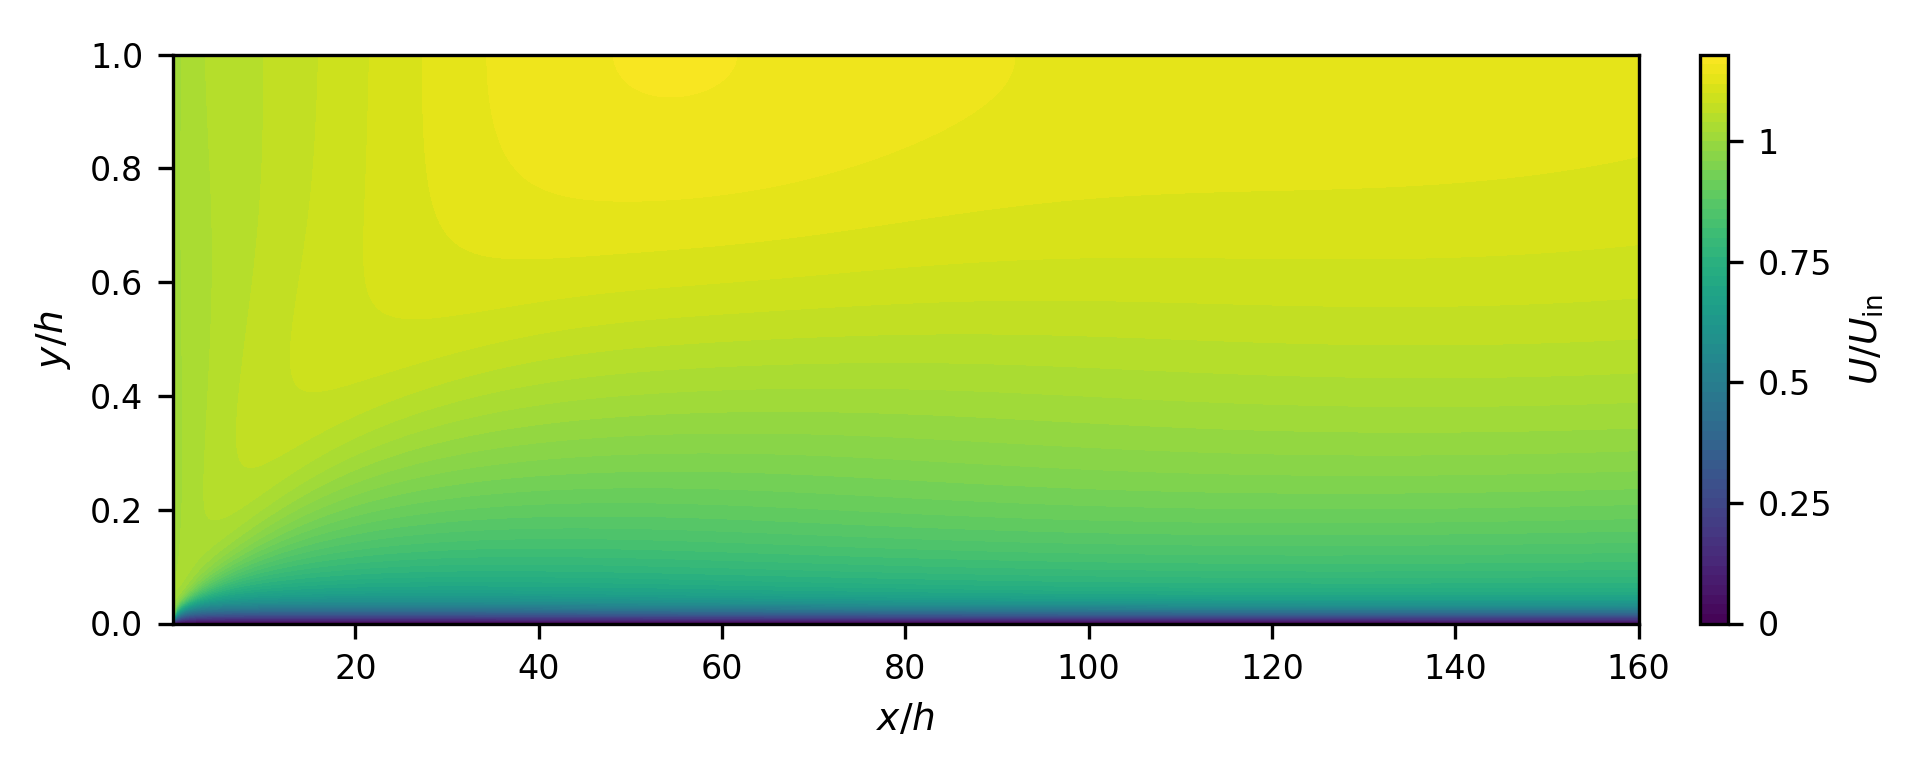
\includegraphics[width=\textwidth]{stage4_pred_U_Re28000.png}
\caption{Streamwise velocity $U / U_{\mathrm{in}}$.}
\end{subfigure}
\hfill
\begin{subfigure}[b]{0.48\textwidth}
\centering
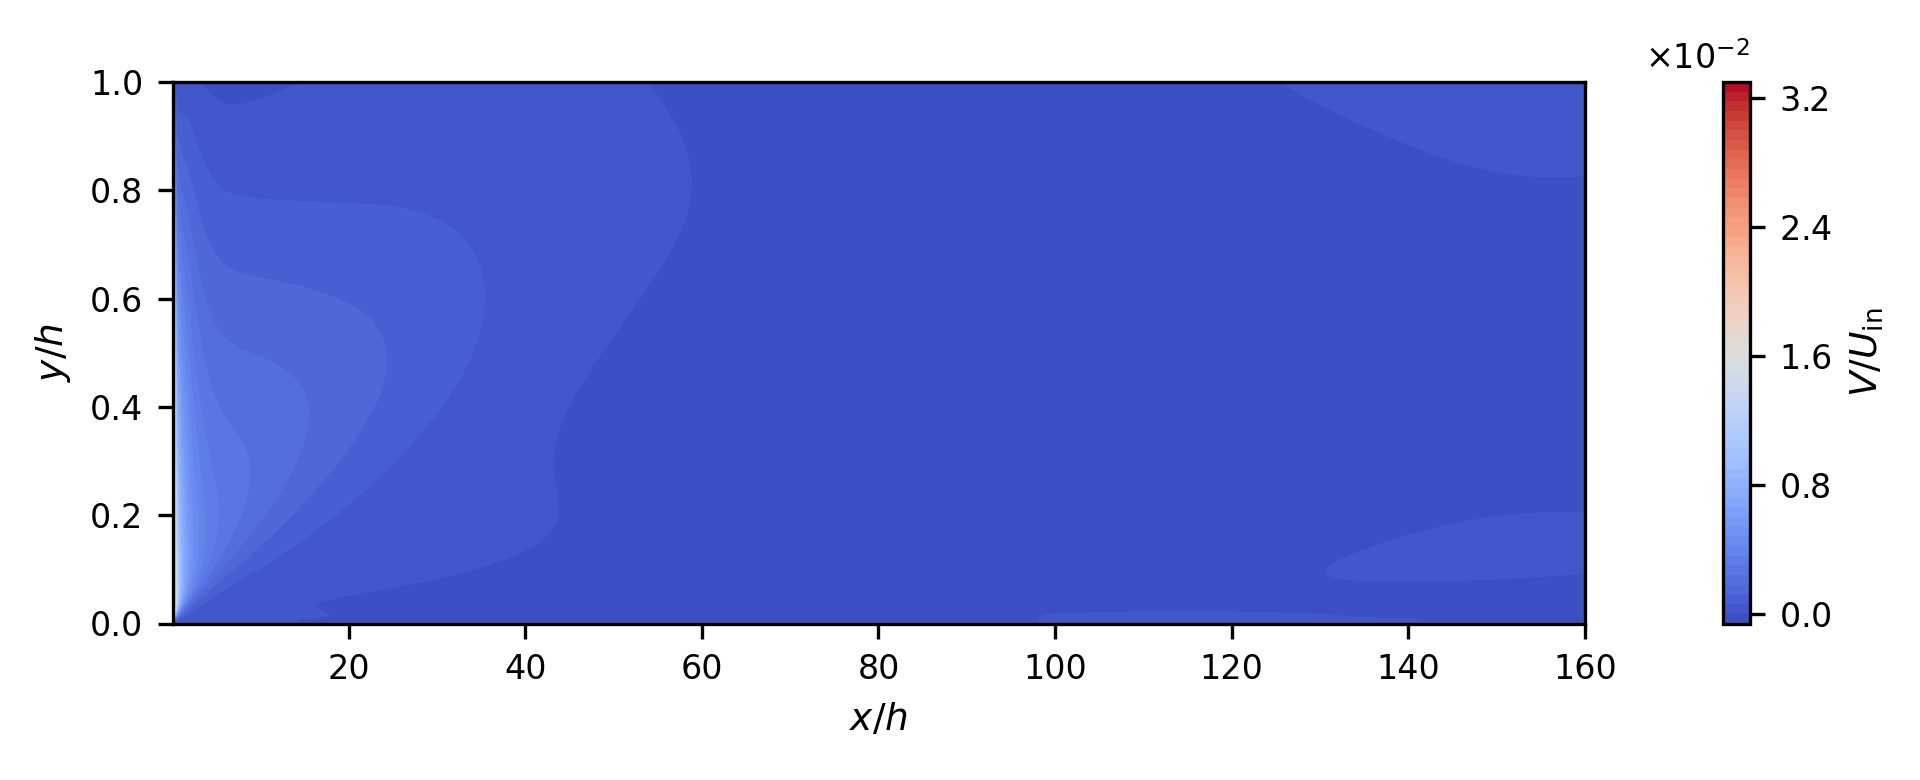
\includegraphics[width=\textwidth]{stage4_pred_V_Re28000.png}
\caption{Wall-normal velocity $V / U_{\mathrm{in}}$.}
\end{subfigure}
\vskip\baselineskip
\begin{subfigure}[b]{0.48\textwidth}
\centering
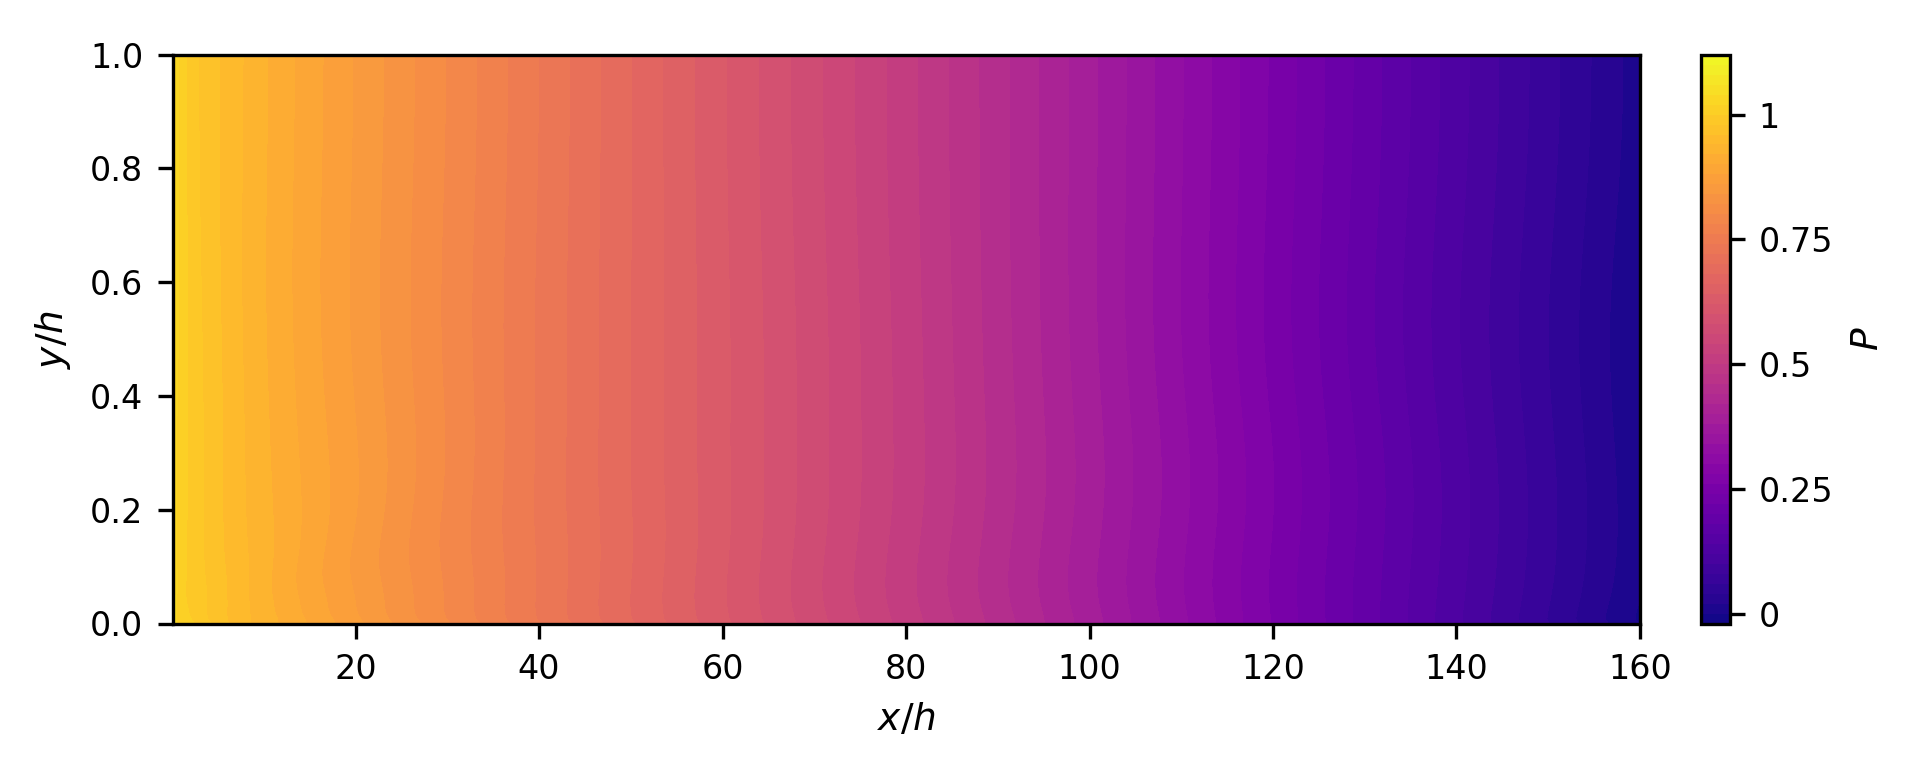
\includegraphics[width=\textwidth]{stage4_pred_P_Re28000.png}
\caption{Dimensionless pressure $P$.}
\end{subfigure}
\hfill
\begin{subfigure}[b]{0.48\textwidth}
\centering
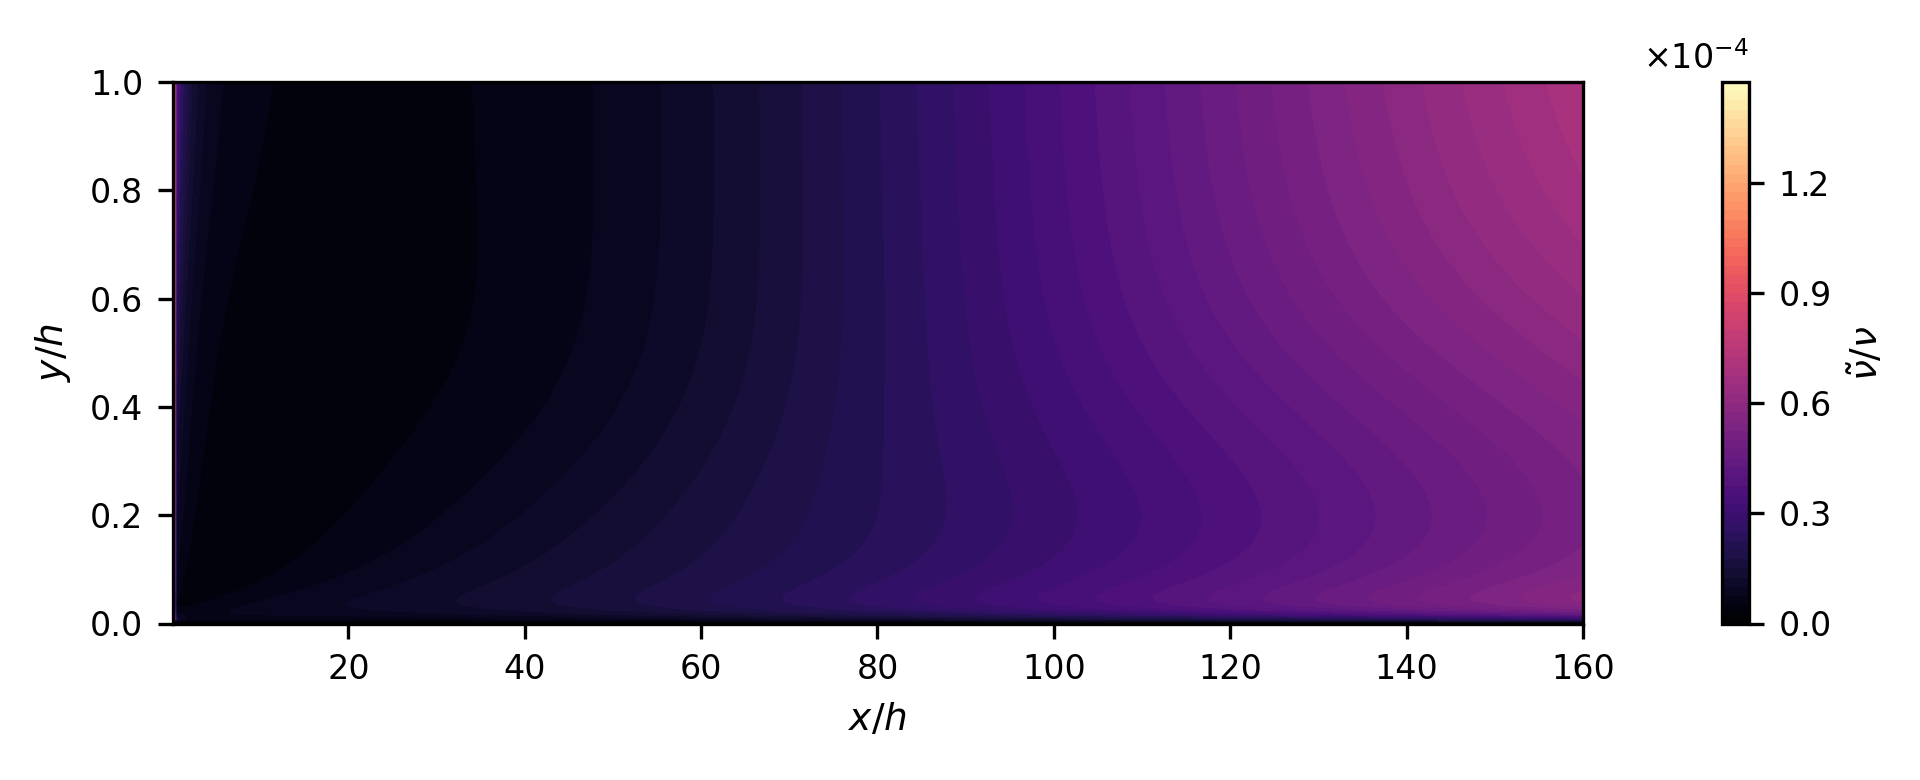
\includegraphics[width=\textwidth]{stage4_pred_nut_Re28000.png}
\caption{Working variable $\tilde{\nu} / \nu$ (network prediction).}
\end{subfigure}
\caption{Stage 4: Predicted turbulent channel flow fields at $\mathrm{Re} = 28{,}000$ (wall-normal axis stretched by a factor $k \approx 57$).}
\label{fig:stage4_pred_re28k}
\end{figure}

\begin{figure}[H]
\centering
\begin{subfigure}[b]{0.48\textwidth}
\centering
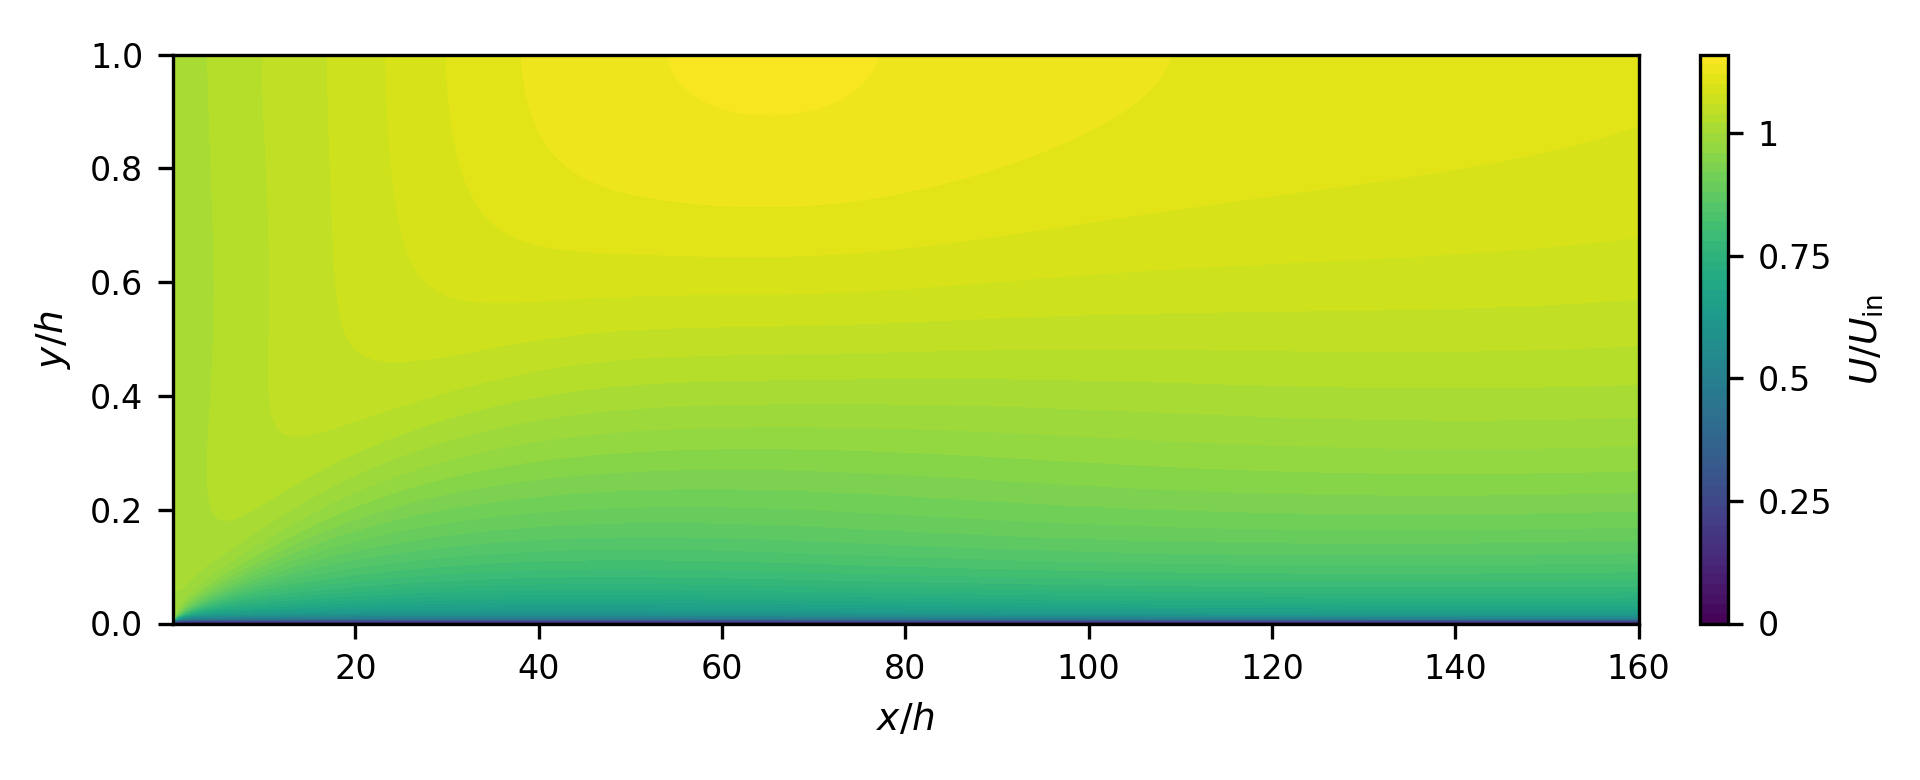
\includegraphics[width=\textwidth]{stage4_pred_U_Re120000.png}
\caption{Streamwise velocity $U / U_{\mathrm{in}}$.}
\end{subfigure}
\hfill
\begin{subfigure}[b]{0.48\textwidth}
\centering
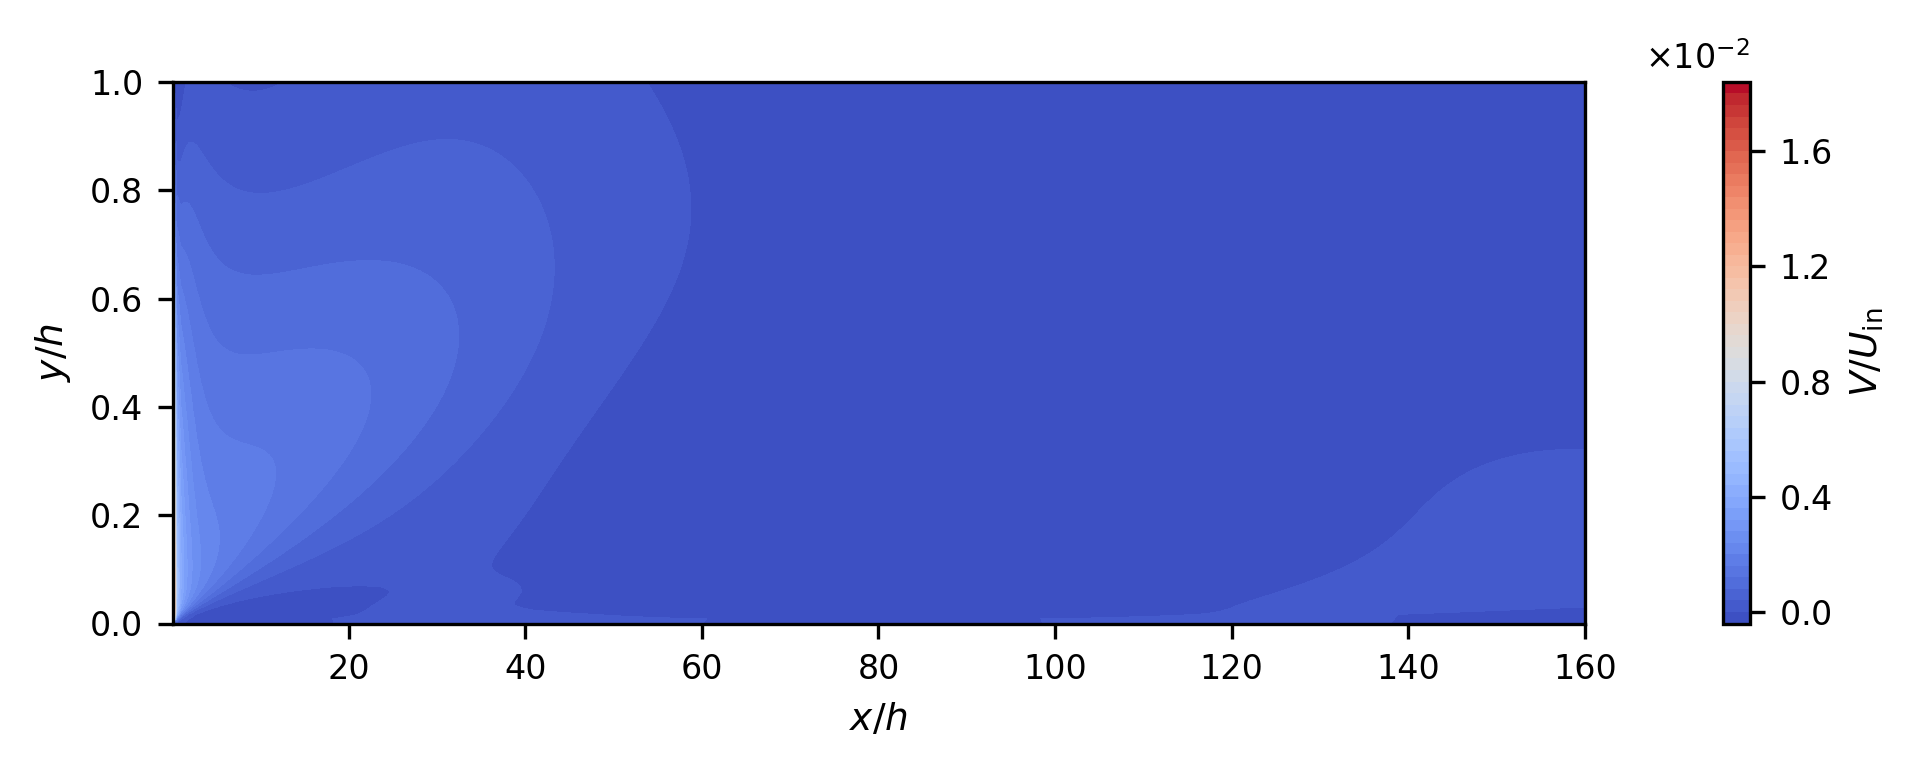
\includegraphics[width=\textwidth]{stage4_pred_V_Re120000.png}
\caption{Wall-normal velocity $V / U_{\mathrm{in}}$.}
\end{subfigure}
\vskip\baselineskip
\begin{subfigure}[b]{0.48\textwidth}
\centering
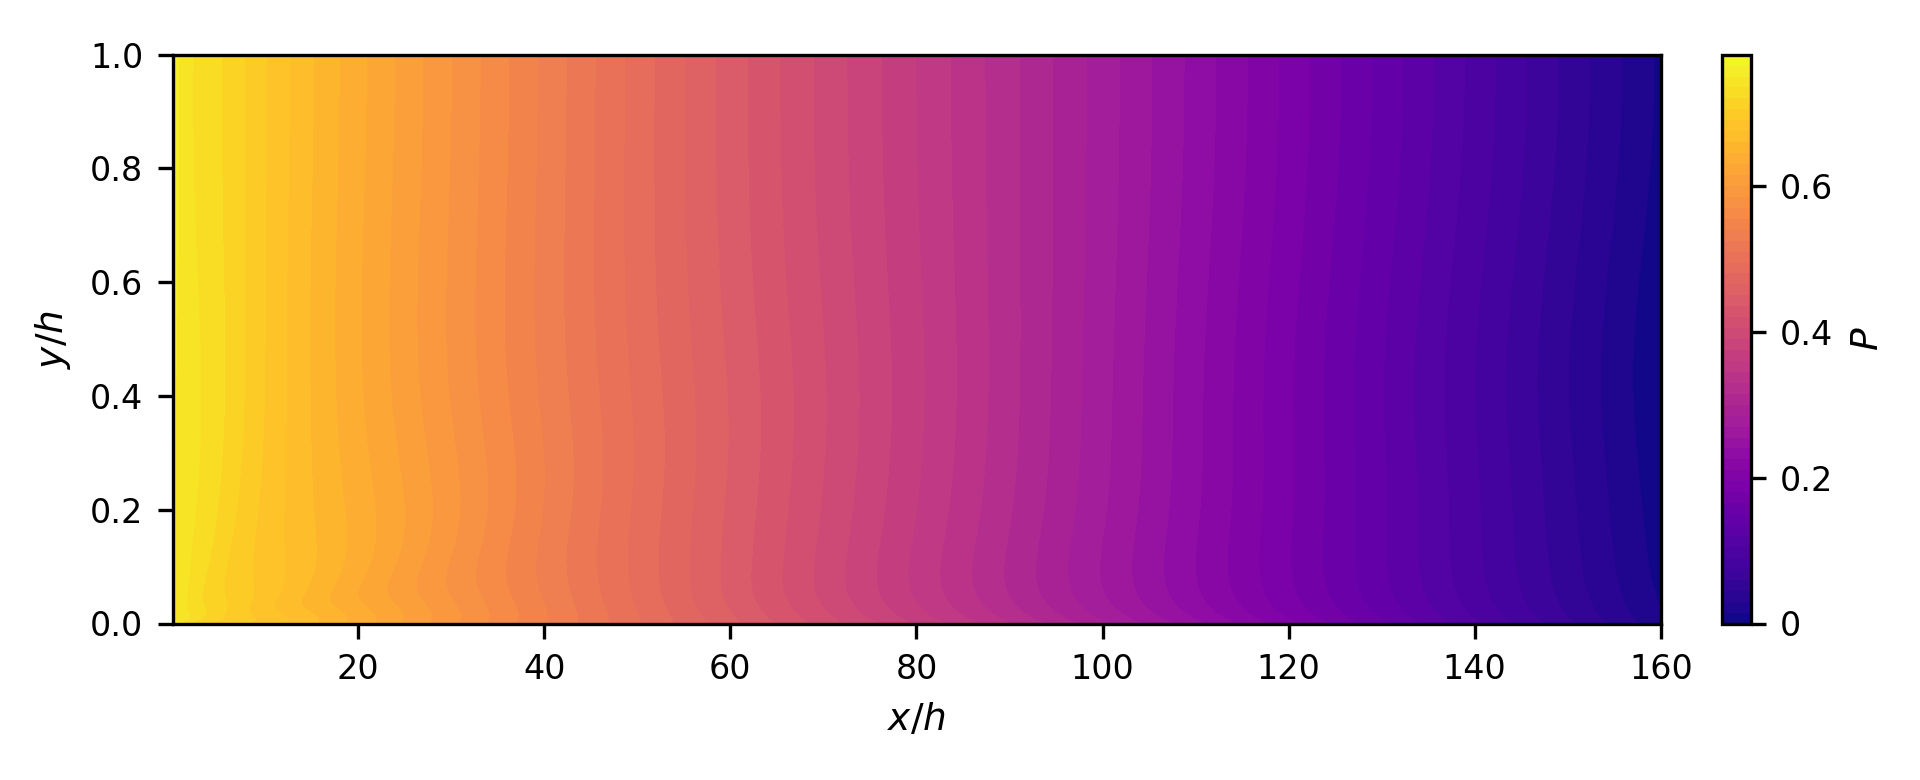
\includegraphics[width=\textwidth]{stage4_pred_P_Re120000.png}
\caption{Dimensionless pressure $P$.}
\end{subfigure}
\hfill
\begin{subfigure}[b]{0.48\textwidth}
\centering
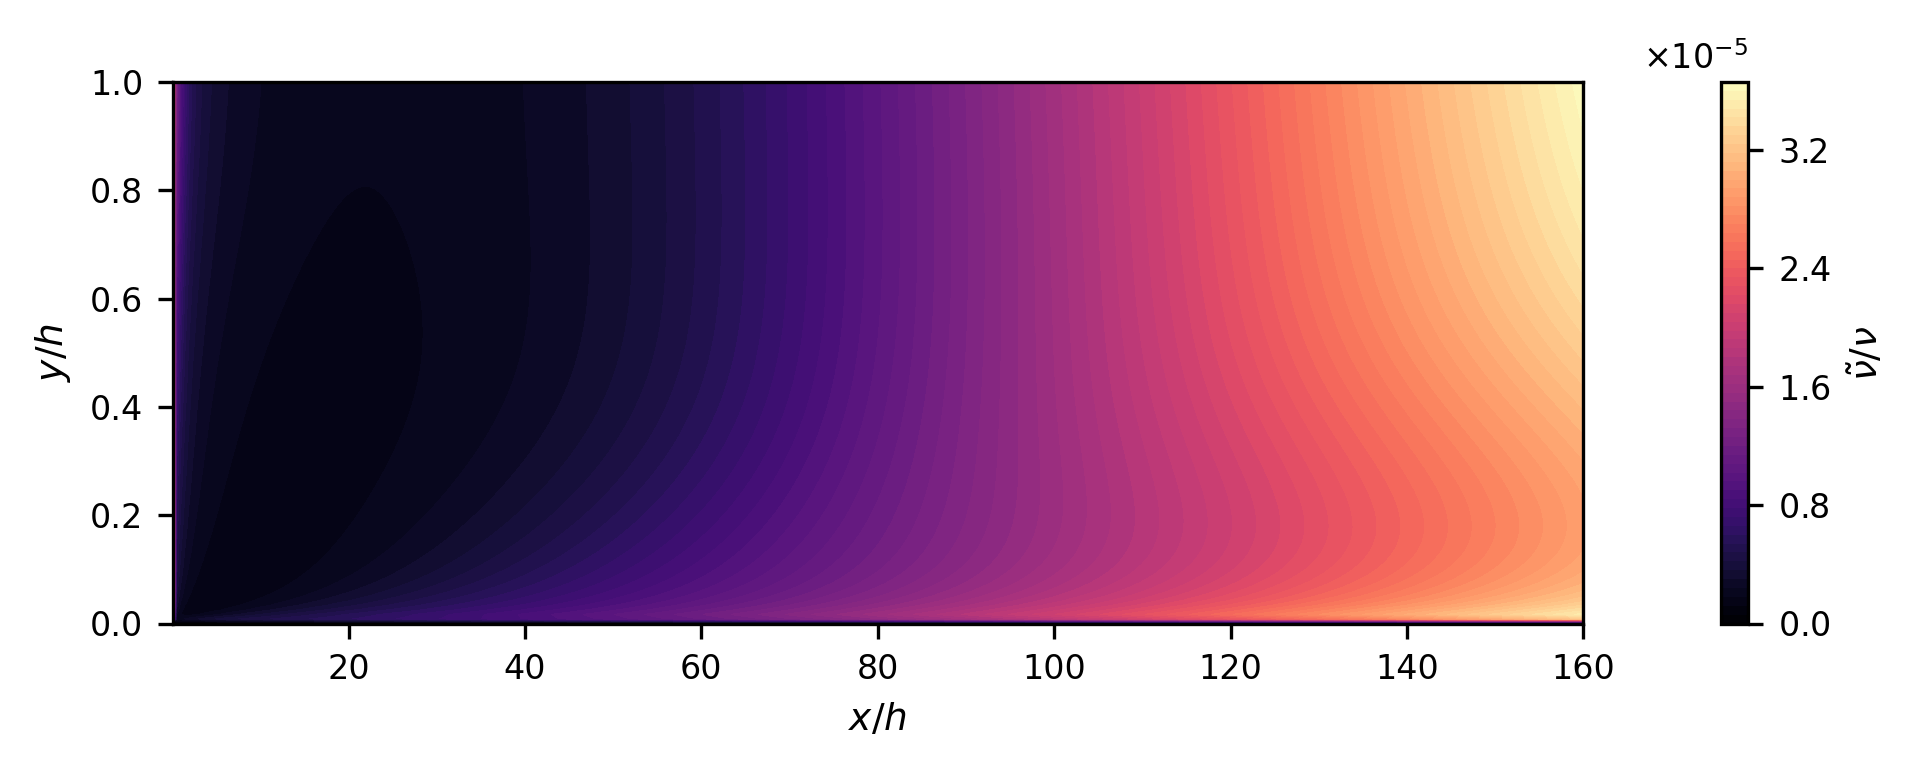
\includegraphics[width=\textwidth]{stage4_pred_nut_Re120000.png}
\caption{Working variable $\tilde{\nu} / \nu$ (network prediction).}
\end{subfigure}
\caption{Stage 4: Predicted turbulent channel flow fields at $\mathrm{Re} = 120{,}000$ (wall-normal axis stretched by a factor $k \approx 57$).}
\label{fig:stage4_pred_re120k}
\end{figure}


\subsection{Discussion: Eddy-Viscosity Variable}
\label{sec:stage4_disc}
\noindent\textbf{Behavior of the Eddy-Viscosity Variable.}
% % src: 4/outputs/final_metrics.csv
Despite accurate mean streamwise velocity ($u$ error $0.42\%$--$0.58\%$; the $v$ error is larger, $6.5\%$--$16.9\%$ at the test Reynolds numbers), the learned turbulent working variable $\tilde{\nu}$ exhibits relative errors of $\mathbf{99.21\%}$ to $\mathbf{99.50\%}$ vs.\ the reference. Over the full domain, the maximum of $\tilde{\nu}/\nu$ in the network prediction is $0.91$ at $\mathrm{Re}=28{,}000$ and $1.09$ at $\mathrm{Re}=120{,}000$ (with domain means of $0.13$ and $0.28$), against reference values reaching $38.48$ and $142.25$ (domain means of $13.52$ and $43.32$). 

This extinction is consistent with the loss weighting, though the root cause was not isolated:
\begin{enumerate}[leftmargin=1.5em]
    \item The training dataset $\mathcal{L}_{\mathrm{data}}$ contained measurements of velocity $(U, V)$ and pressure $P$, but contained \textit{zero direct supervision on $\tilde{\nu}$}. The weights were chosen by the Optuna search scored on data accuracy; the eddy-viscosity field is not part of the training data, so only the physics terms constrain it.
    \item The Optuna search selected a large weight for the data term ($w_{\mathrm{data}} \approx 6768.75$) and very small weights for the physics residuals: the turbulence-equation (SA) loss weight ratio is $w_{\mathrm{sa}}/w_{\mathrm{data}} \approx 4.89\times 10^{-9}$ ($3.31\times 10^{-5}/6768.75$), while the momentum weight ratio is $w_{\mathrm{mom}}/w_{\mathrm{data}} \approx 5.08\times 10^{-9}$ ($3.44\times 10^{-5}/6768.75$).
\end{enumerate}
With molecular viscosity $\nu$ alone sufficient for the flexible MLP to fit the boundary-layer velocity data, the result is consistent with the network minimizing the dominant data loss while leaving $\tilde{\nu} \approx 0$; no ablation isolates this cause.

\begin{figure}[H]
\centering
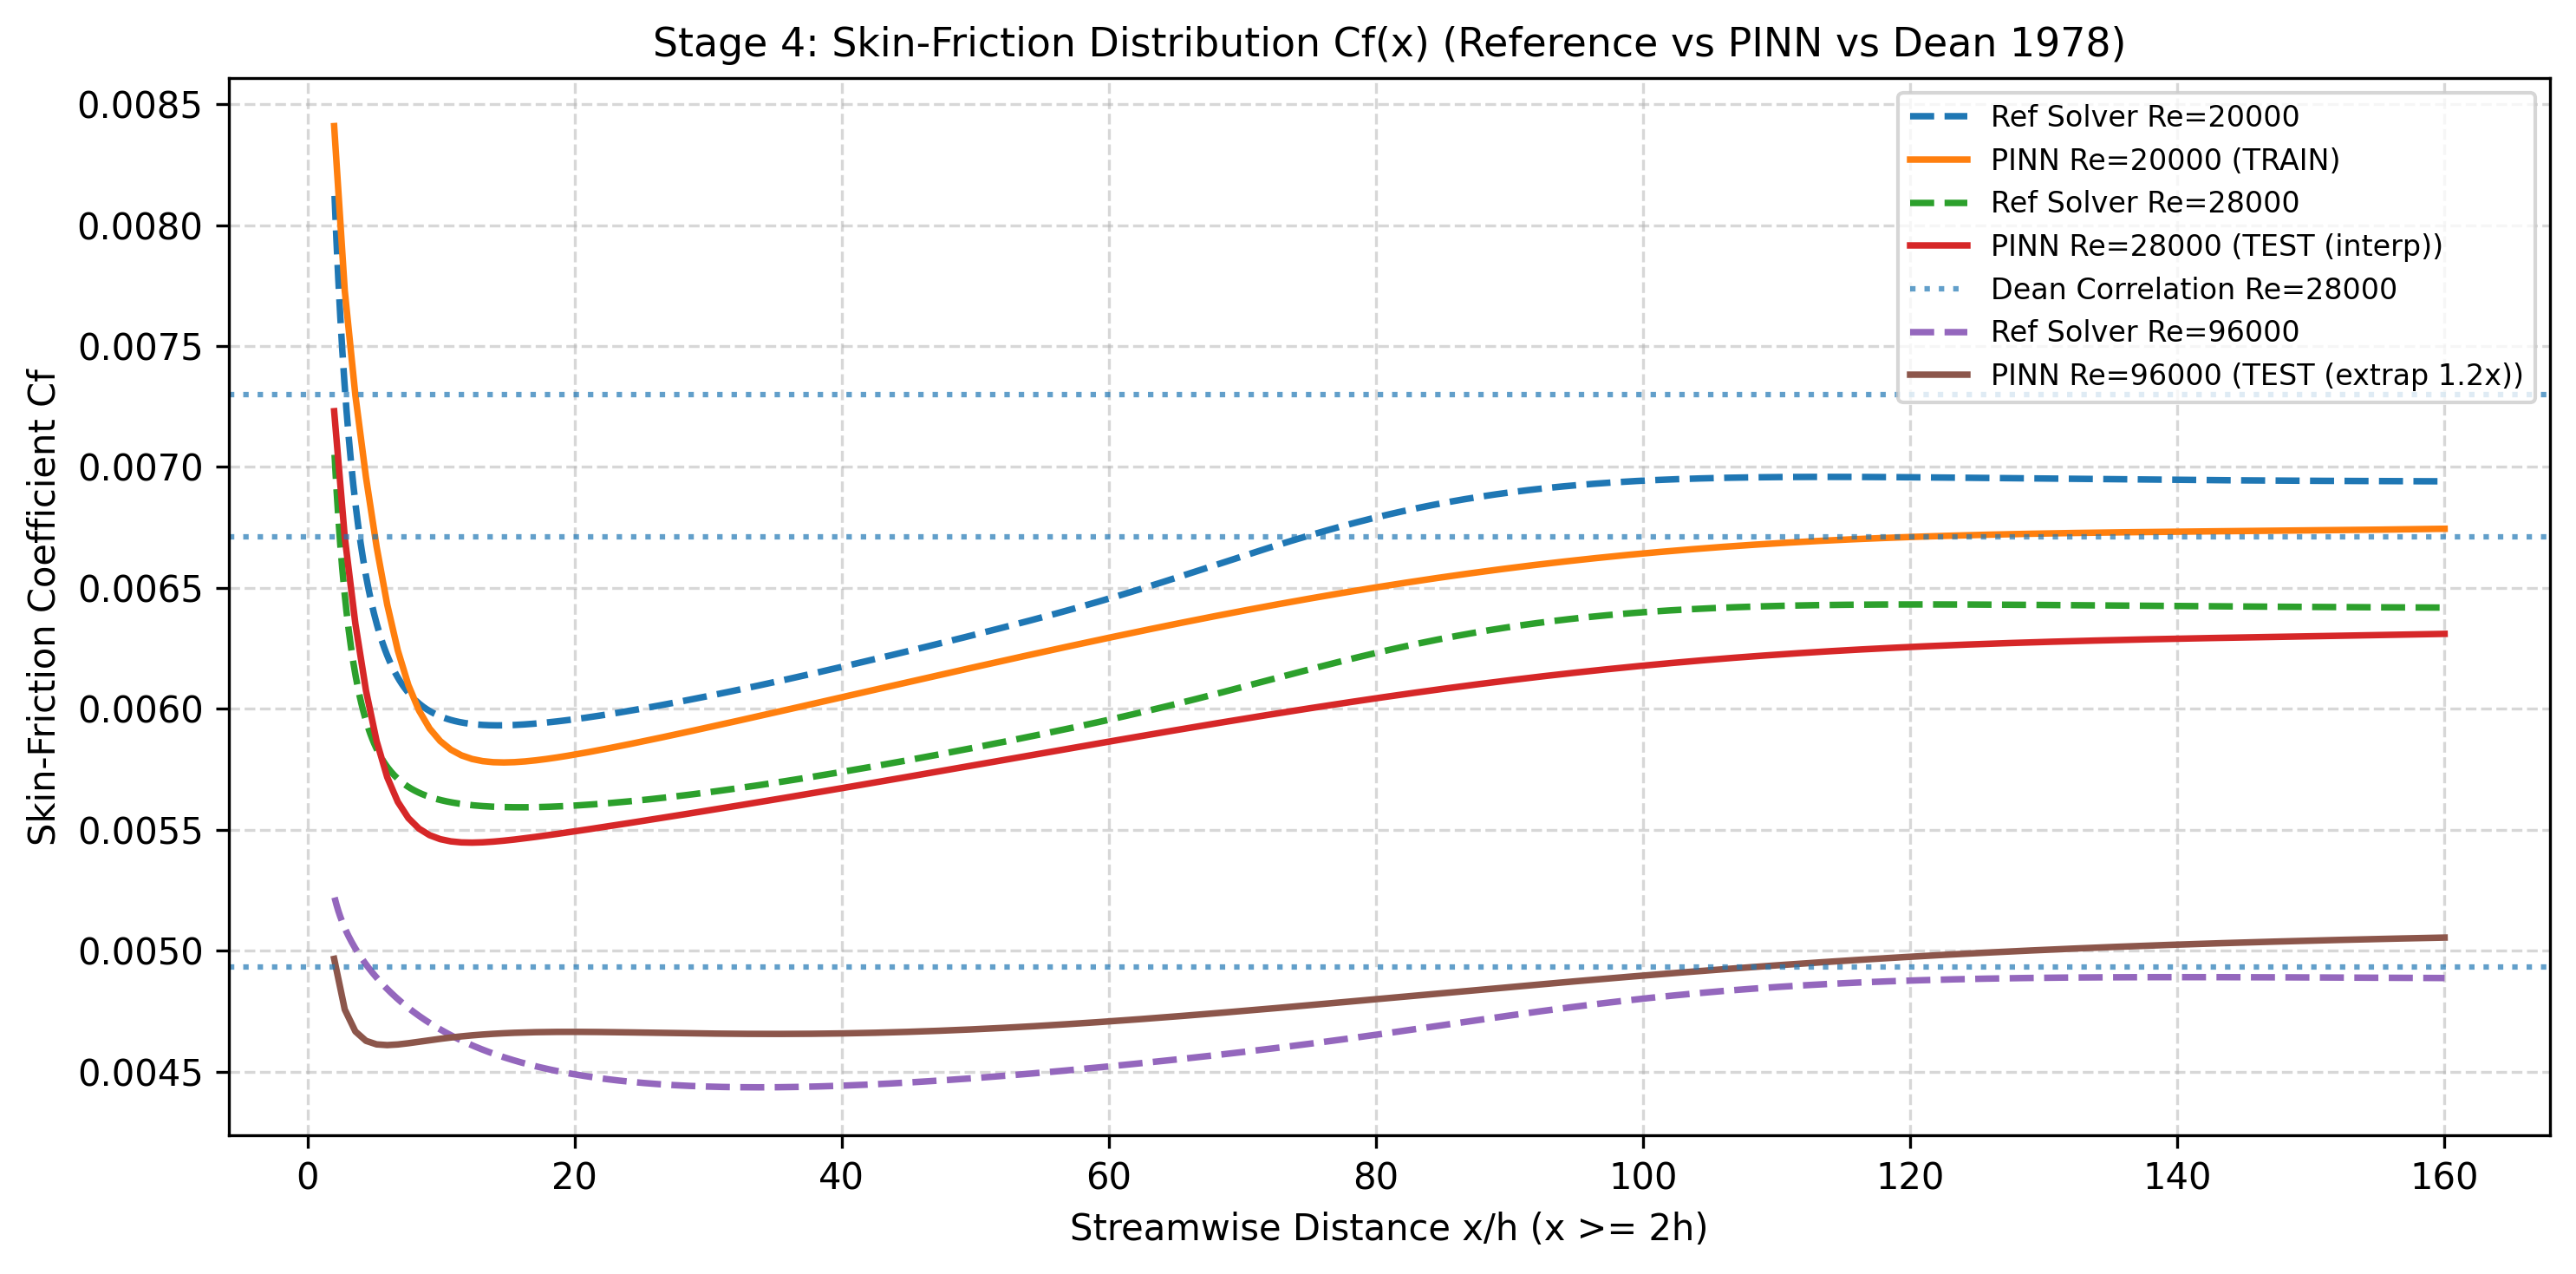
\includegraphics[width=\textwidth]{channel_turb_skin_friction_cf_comparison.png}
\caption{Stage 4: Skin friction coefficient $C_f(x)$ comparison between PINN, reference solver, and Dean-type empirical correlation.}
\label{fig:stage4_cf}
\end{figure}

% ==============================================================================
% SECTION 7: STAGE 5
% ==============================================================================
\section{Stage 5: Developing Turbulent Pipe Flow and Superpipe Validation}
\label{sec:stage5}

\subsection{Geometry and Physical Problem Setup}
Stage 5 investigates developing turbulent flow in a circular pipe ($L/R = 160, \mathrm{Re} \in [10^4, 1.2\times 10^5]$). Non-dimensionalization sets pipe radius $R = 1.0$ and bulk velocity $U_b = 1.0$. The computational domain spans $(x, r) \in [0, 160] \times [0, 1]$. Kinematic viscosity is $\nu = 2/\mathrm{Re}$.

\begin{figure}[H]
\centering
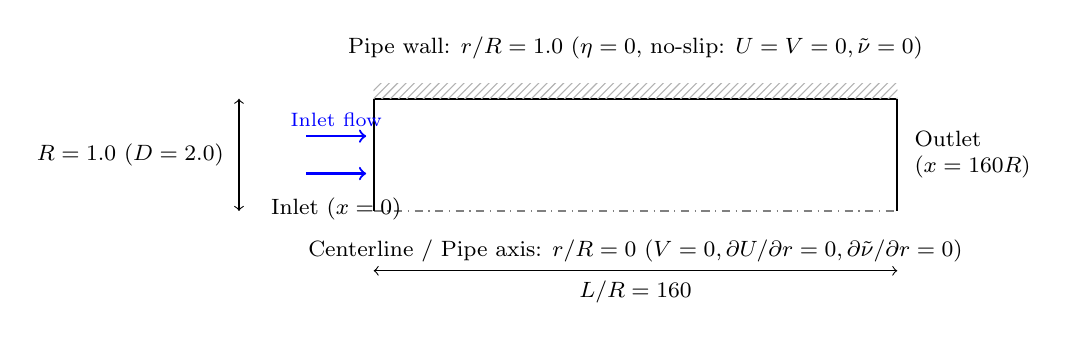
\begin{tikzpicture}[scale=0.95]
    \node[above, font=\footnotesize] at (3.5, 1.9) {Pipe wall: $r/R = 1.0$ ($\eta = 0$, no-slip: $U=V=0, \tilde{\nu}=0$)};
    \draw[thick] (0, 1.5) -- (7.0, 1.5);
    \fill[pattern=north east lines, pattern color=gray!60] (0, 1.5) rectangle (7.0, 1.7);
    \draw[dashdotted, thick, gray] (0, 0) -- (7.0, 0);
    \node[below, font=\footnotesize] at (3.5, -0.25) {Centerline / Pipe axis: $r/R = 0$ ($V=0, \partial U/\partial r = 0, \partial \tilde{\nu}/\partial r = 0$)};
    \draw[thick] (0, 0) -- (0, 1.5);
    \draw[blue, thick, ->] (-0.9, 1.0) -- (-0.1, 1.0);
    \draw[blue, thick, ->] (-0.9, 0.5) -- (-0.1, 0.5);
    \node[blue, font=\scriptsize, above] at (-0.5, 1.0) {Inlet flow};
    \node[font=\footnotesize, below] at (-0.5, 0.3) {Inlet ($x=0$)};
    \draw[thick] (7.0, 0) -- (7.0, 1.5);
    \node[right, font=\footnotesize, align=left] at (7.1, 0.75) {Outlet\\($x=160R$)};
    \draw[<->] (0, -0.8) -- (7.0, -0.8) node[midway, below, font=\footnotesize] {$L/R = 160$};
    \draw[<->] (-1.8, 0) -- (-1.8, 1.5) node[midway, left=2pt, font=\footnotesize] {$R = 1.0$ ($D = 2.0$)};
\end{tikzpicture}
\caption{Stage 5 geometry: turbulent pipe domain ($r/R \in [0, 1.0]$).}
\label{fig:stage5_geom}
\end{figure}

\subsection{Governing Equations and Axisymmetric Cylindrical RANS+SA System}
The axisymmetric cylindrical RANS equations are:
\begin{align}
\label{eq:pipe_rans_cont}
\frac{\partial U}{\partial x} + \frac{1}{r}\frac{\partial (r V)}{\partial r} &= 0, \\
\label{eq:pipe_rans_mom_x}
U \frac{\partial U}{\partial x} + V \frac{\partial U}{\partial r} &= -\frac{\partial P}{\partial x} + \frac{\partial}{\partial x}\left(2\nu_{\mathrm{eff}}\frac{\partial U}{\partial x}\right) + \frac{1}{r}\frac{\partial}{\partial r}\left(r \nu_{\mathrm{eff}}\left(\frac{\partial U}{\partial r} + \frac{\partial V}{\partial x}\right)\right), \\
\label{eq:pipe_rans_mom_r}
U \frac{\partial V}{\partial x} + V \frac{\partial V}{\partial r} &= -\frac{\partial P}{\partial r} + \frac{\partial}{\partial x}\left(\nu_{\mathrm{eff}}\left(\frac{\partial U}{\partial r} + \frac{\partial V}{\partial x}\right)\right) + \frac{1}{r}\frac{\partial}{\partial r}\left(2 r \nu_{\mathrm{eff}}\frac{\partial V}{\partial r}\right) - 2\nu_{\mathrm{eff}}\frac{V}{r^2}.
\end{align}
The SA working variable $\tilde{\nu}$ satisfies:
\begin{equation}
\label{eq:pipe_rans_sa}
\begin{split}
U \frac{\partial \tilde{\nu}}{\partial x} + V \frac{\partial \tilde{\nu}}{\partial r} = c_{b1} \tilde{S} \tilde{\nu} - c_{w1} f_w \left(\frac{\tilde{\nu}}{d}\right)^2 &+ \frac{1}{\sigma}\left[ \frac{\partial}{\partial x}\left((\nu+\tilde{\nu})\frac{\partial \tilde{\nu}}{\partial x}\right) + \frac{1}{r}\frac{\partial}{\partial r}\left(r (\nu+\tilde{\nu})\frac{\partial \tilde{\nu}}{\partial r}\right) \right. \\
&\quad\left. +\, c_{b2}\left(\left(\frac{\partial \tilde{\nu}}{\partial x}\right)^2 + \left(\frac{\partial \tilde{\nu}}{\partial r}\right)^2\right) \right].
\end{split}
\end{equation}
The eddy viscosity is $\nu_t = \tilde{\nu} f_{v1}$ and $\nu_{\mathrm{eff}} = \nu + \nu_t$. Standard NASA Turbulence Modeling Resource closure definitions in cylindrical coordinates are:
\begin{align}
\chi &= \frac{\tilde{\nu}}{\nu}, \quad f_{v1} = \frac{\chi^3}{\chi^3 + c_{v1}^3}, \quad f_{v2} = 1 - \frac{\chi}{1 + \chi f_{v1}}, \\
\tilde{S} &= S + \frac{\tilde{\nu}}{\kappa^2 d^2} f_{v2}, \quad S = \left|\frac{\partial U}{\partial r} - \frac{\partial V}{\partial x}\right|, \quad r_d = \min\left(\frac{\tilde{\nu}}{\tilde{S}\kappa^2 d^2}, 10\right), \\
g_w &= r_d + c_{w2}(r_d^6 - r_d), \quad f_w = g_w \left(\frac{1 + c_{w3}^6}{g_w^6 + c_{w3}^6}\right)^{1/6},
\end{align}
where $d = 1 - r$ denotes normal distance to the pipe wall, and empirical model constants are $c_{b1} = 0.1355$, $c_{b2} = 0.622$, $\sigma = 2/3$, $\kappa = 0.41$, $c_{w1} = c_{b1}/\kappa^2 + (1+c_{b2})/\sigma$, $c_{w2} = 0.3$, $c_{w3} = 2.0$, and $c_{v1} = 7.1$. Turbulent pipe flow friction law and DNS velocity benchmarks are documented by Pirozzoli et al.~\cite[Eq.~(3.2), p.~7]{pirozzoli2021}.

\subsection{Reference Marching Solver and Discretization}
Reference data was computed with an independent axisymmetric marching code (\texttt{5/reference\_}\allowbreak\texttt{solver.py}) on an $800 \times 400$ wall-stretched grid ($N_X = 800, N_R = 400$). The reference solver solves the parabolized cylindrical boundary-layer equations:
\begin{align}
\frac{\partial U}{\partial x} + \frac{1}{r}\frac{\partial(r V)}{\partial r} &= 0, \\
U \frac{\partial U}{\partial x} + V \frac{\partial U}{\partial r} &= -\frac{dP}{dx} + \frac{1}{r}\frac{\partial}{\partial r}\left(r \nu_{\mathrm{eff}}\frac{\partial U}{\partial r}\right), \\
U \frac{\partial \tilde{\nu}}{\partial x} + V \frac{\partial \tilde{\nu}}{\partial r} &= c_{b1}\tilde{S}\tilde{\nu} - c_{w1}f_w\left(\frac{\tilde{\nu}}{d}\right)^2 + \frac{1}{\sigma}\frac{1}{r}\frac{\partial}{\partial r}\left(r (\nu+\tilde{\nu})\frac{\partial \tilde{\nu}}{\partial r}\right) + \frac{c_{b2}}{\sigma}\left(\frac{\partial \tilde{\nu}}{\partial r}\right)^2.
\end{align}
% src: 5/reference_solver.py:10-40; 5/config.py:30-32
\noindent\textbf{Terms Dropped in Parabolic Formulation:}\\[0.2em]
The marching solver drops all axial diffusion ($\partial^2 U/\partial x^2 = 0$, $\partial^2 \tilde{\nu}/\partial x^2 = 0$) and drops radial momentum balance ($\partial P/\partial r = 0 \implies P = P(x)$). Constant volumetric mass flux $2\int_0^1 U r\,dr = 1$ is maintained via pressure-gradient superposition ($U = U_a - \frac{dP}{dx} U_b$).

\noindent\textbf{Discretization and Computational Grid:} Spatial discretization uses implicit axial marching with a damped Levenberg--Marquardt Newton iteration at each streamwise station. The computational mesh comprises $N_X = 800$ axial stations (power-law clustered near the inlet) and $N_R = 400$ wall-stretched radial cells (tanh-stretched with $y^+ < 1.0$ at $r=1.0$).

As noted in Section~\ref{sec:elliptic_vs_parabolic}, the reference solver is parabolic, whereas the PINN enforces the full elliptic cylindrical RANS system (Eqs.~\eqref{eq:pipe_rans_cont}--\eqref{eq:pipe_rans_sa}); the resulting difference is largest near the inlet.

\subsection{Network Design, Features, and Cylindrical Envelopes}
% src: 5/pinn.py:64-68
The neural network (\texttt{5/pinn.py}, class \texttt{PipePINN}) employs an MLP with four hidden layers of 64 neurons (13,060 parameters). Inputs are four features rescaled to $[-1, 1]$ with wall distance $\eta = 1 - r$:
\begin{equation}
f_1 = 2\sqrt{\frac{x}{L}} - 1, \quad f_2 = 2\eta - 1, \quad f_3 = 2\frac{\ln(1 + \mathrm{Re}_\tau \eta)}{\ln(1 + \mathrm{Re}_\tau)} - 1, \quad f_4 = \frac{\log_{10} \mathrm{Re} - 4.4515}{0.4515}.
\end{equation}
At the extrapolation Reynolds numbers $f_4$ exceeds 1 (1.18 at $\mathrm{Re} = 96{,}000$ and 1.39 at $\mathrm{Re} = 120{,}000$).
Cylindrical hard boundary envelopes enforce exact wall no-slip, centerline symmetry, and positivity:
\begin{align}
% src: 5/pinn.py:79-84
g(\eta) &= \tanh\left(\frac{\mathrm{Re}_\tau \eta}{10}\right), \\
U &= g(\eta)\,(1 + a_0), \quad V = (V_{\mathrm{scale}} u_\tau)\,g(\eta)^2\,r\,a_1, \quad \hat{P} = a_2, \quad \tilde{\nu} = \nu\,\mathrm{Re}_\tau\,g(\eta)\,\operatorname{softplus}(a_3 - 3.0),
\end{align}
where $u_\tau = \sqrt{\frac{1}{2}\times 0.0791 \mathrm{Re}^{-0.25}}$ (Blasius-type friction constant for the pipe; Stage 4 uses the Dean-type constant $0.073$ for the channel), $V_{\mathrm{scale}} = 0.10$, and $\nu = 2/\mathrm{Re}$. Centerline regularity $V(r=0) = 0$ is enforced by the explicit factor $r$.
% src: 5/config.py:71; 5/train.py:124; 5/search_weights.py
Optimization uses Adam for 12,000 iterations (initial learning rate $8.40\times 10^{-3}$, exponential decay $100\times$) followed by 200 iterations of L-BFGS polish. At each iteration, $N_{\mathrm{data}} = 2{,}048$ data points are sampled from the reference pool, and $N_{\mathrm{pde}} = 2{,}048$ collocation points are drawn anew with log-uniform near-wall clustering in $y^+$. Collocation counts per iteration are 2,048 data points, 2,048 interior PDE points, and 512 boundary points. Optimal loss weights were discovered using Optuna TPE Bayesian optimization.

\subsection{Composite Loss Formulation and Final Weights}
The Stage 5 loss function incorporates identical objective terms to Stage 4. The final weights read from \texttt{5/outputs/best\_weights\_dense.json} are:
\begin{align}
% src: 5/outputs/best_weights_dense.json
w_{\mathrm{data}} &= 1996.58, \quad w_{\mathrm{mom}} = 5.52\times 10^{-4}, \quad w_{\mathrm{sa}} = \mathbf{2.233}, \quad w_{\mathrm{cont}} = 11.82, \\
w_{v} &= 0.015, \quad w_{p} = 0.363, \quad w_{\mathrm{in}} = 1.515, \quad w_{\mathrm{out}} = 2.055, \quad w_{\mathrm{sym}} = 0.359.
\end{align}
\noindent\textbf{Comparison of Loss Weights Between Stages:} The relative SA physics-to-data weight ratio is:
\begin{equation}
\frac{w_{\mathrm{sa}}}{w_{\mathrm{data}}} = \frac{2.233}{1996.58} \approx \mathbf{1.12\times 10^{-3}},
\end{equation}
which is about $2.3\times 10^5$ times larger than the Stage~4 SA ratio ($w_{\mathrm{sa}}/w_{\mathrm{data}} \approx 4.89\times 10^{-9}$), while the momentum ratio ($w_{\mathrm{mom}}/w_{\mathrm{data}} \approx 2.76\times 10^{-7}$) is about $54\times$ larger than in Stage~4 ($5.08\times 10^{-9}$).

\subsection{Forward Pass at a Single Point}
The pre-activation vector $z = W a_{\mathrm{prev}} + b$ represents the affine combination entering each layer, while the post-activation $a = \tanh(z)$ is its bounded output. Matrix $\|W\|_F$ denotes the Frobenius norm of the layer weight matrix, $\|b\|_2$ is the Euclidean norm of the bias vector, and $z[1:4]$ reports the numerical values of the first four neurons of each layer.

Table~\ref{tab:stage5_act} reports the deterministic forward pass evaluated from the Stage~5 dense checkpoint at $(x=40R, r=0.5R, \mathrm{Re}=40{,}000)$.
\begin{table}[H]
\centering
\resizebox{\linewidth}{!}{%
\begin{tabular}{lcccc}
\toprule
\textbf{Network Layer} & \textbf{Pre-activations} $z_{[1:4]}$ & \textbf{Post-activations} $a_{[1:4]} = \tanh(z)$ & $\|W\|_F$ & $\|b\|_2$ \\
\midrule
Hidden 1 & $[-0.2267, 0.3997, 0.2123, 0.3520]$ & $[-0.2229, 0.3797, 0.2091, 0.3382]$ & 4.24 & 2.41 \\
Hidden 2 & $[1.7690, -1.0227, 1.5966, -4.9825]$ & $[0.9435, -0.7710, 0.9212, -0.9999]$ & 13.35 & 1.71 \\
Hidden 3 & $[3.0137, -0.7519, 0.4437, -0.0928]$ & $[0.9952, -0.6363, 0.4167, -0.0925]$ & 12.81 & 1.23 \\
Hidden 4 & $[2.0068, -0.4525, -2.8995, -0.6122]$ & $[0.9645, -0.4240, -0.9940, -0.5457]$ & 10.87 & 1.51 \\
Output & $[0.1523, -0.1620, 1.3229, -1.4583]$ & N/A & 5.37 & 0.57 \\
\bottomrule
\end{tabular}%
}
\caption{Deterministic layer-by-layer forward pass evaluated at $(x=40R, r=0.5R, \mathrm{Re}=40{,}000)$. Normalized input vector: $[0.0000, 0.0000, 0.8010, 0.3335]^{\mathsf T}$. Checkpoint SHA256: \texttt{82a6cf755909e86e...}.}
\label{tab:stage5_act}
\end{table}
Envelopes yield physical predictions:
\begin{align}
% src: verify_forward_pass.py; 5/outputs/models/dense/final_seed0.pt
U &= \mathbf{1.15230} \quad (\text{reference: } 1.14827, \text{ error } 0.35\%), \\
V &= -0.00045 \quad (\text{reference: } -1.2\times 10^{-6}), \\
P &= \mathbf{1.32287} \quad (\text{reference: } 1.31942, \text{ error } 0.26\%), \\
\tilde{\nu} &= \mathbf{0.000604} \quad (\text{reference: } 0.002364, \text{ error } \mathbf{74.47\%}).
\end{align}

\subsection{Empirical Results, Radial Profiles, and Princeton Superpipe Validation}
Table~\ref{tab:stage5_metrics} compiles quantitative errors across all evaluated Reynolds numbers.
\begin{table}[H]
\centering
\resizebox{\textwidth}{!}{
\begin{tabular}{lccc}
\toprule
\textbf{Metric Variable} & $\mathbf{Re=28{,}000}$ (TEST-interp) & $\mathbf{Re=96{,}000}$ (TEST-extrap 1.2$\times$) & $\mathbf{Re=120{,}000}$ (TEST-extrap 1.5$\times$) \\
\midrule
$u$ (Axial Velocity Rel $L_2$) & 0.36\% & 0.38\% & 0.57\% \\
$v$ (Radial Velocity Rel $L_2$) & 4.69\% & 2.87\% & 4.47\% \\
$p$ (Kinematic Pressure Rel $L_2$) & 0.65\% & 0.98\% & 2.57\% \\
$C_f$ (Skin Friction Rel Error) & 1.47\% & 1.77\% & 2.24\% \\
$\tilde{\nu}$ (Eddy Viscosity Whole-Domain Rel $L_2$) & 47.11\% & 77.23\% & 79.64\% \\
$\tilde{\nu}$ (Eddy Viscosity Exit $x=160R$ Rel $L_2$) & 51.98\% & 79.39\% & 81.11\% \\
\bottomrule
\end{tabular}
}
\caption{Stage 5: Exact quantitative test metrics for axisymmetric turbulent pipe flow (Source: \texttt{5/outputs/eval\_dense\_final\_test.json} and checkpoint evaluation). $C_f$ error is the relative error of the wall shear stress coefficient with respect to the reference solver.}
\label{tab:stage5_metrics}
\end{table}


% % src: 5/outputs/eval_dense_final_test.json
Velocity errors range between $0.36\%$ and $0.57\%$ . For skin friction, the PINN agrees within $1.47\%$--$2.24\%$ relative error against the reference solver across the test Reynolds numbers (Table~\ref{tab:stage5_metrics}) and within $1.22\%$--$4.65\%$ against the smooth-pipe friction law ($1/\lambda^{1/2} = 2.102\log_{10}(\mathrm{Re}_b \lambda^{1/2}) - 1.148$, with $C_f = \lambda/4$~\cite[Eq.~(3.2), p.~7]{pirozzoli2021}). At $\mathrm{Re} = 120{,}000$ ($x = 160R$), the fully developed skin friction is $C_f^{\mathrm{PINN}} = 0.004449$, the reference solver gives $C_f^{\mathrm{ref}} = 0.004441$ (difference $0.18\%$), and the friction law gives $C_f = 0.004251$ (difference $4.65\%$).

\noindent\textbf{Experimental Validation Against Princeton Superpipe Traverses:}
% % src: tables/table_c3_superpipe.tex: minimum $2.81\%$ for dataset \texttt{zag\_1.4579E+05.txt}, maximum $4.18\%$ for dataset \texttt{mck\_1.4458E+05.txt}
The network was benchmarked directly against eight high-precision Pitot traverse datasets from the Princeton Superpipe experiment~\cite{superpipe_data} spanning $\mathrm{Re} = 31{,}577$ to $145{,}790$. The two datasets at $\mathrm{Re} = 144{,}580$ and $145{,}790$ lie above the largest Reynolds number used in the test split ($120{,}000$). Table~\ref{tab:superpipe_all_re} in Appendix~\ref{sec:app_tables} presents complete metrics. Across all eight experimental profiles, the relative $L_2$ error spans $\mathbf{2.81\%}$ to $\mathbf{4.18\%}$. The Superpipe profiles are Pitot-tube measurements; the probe-size and static-pressure corrections are described in the data source~\cite{superpipe_data}. The comparison tests the mean velocity profile of the network; it does not by itself validate the Spalart--Allmaras eddy-viscosity closure, whose predicted eddy viscosity still differs from the reference solver (Table~\ref{tab:stage5_metrics}).

\begin{figure}[H]
\centering
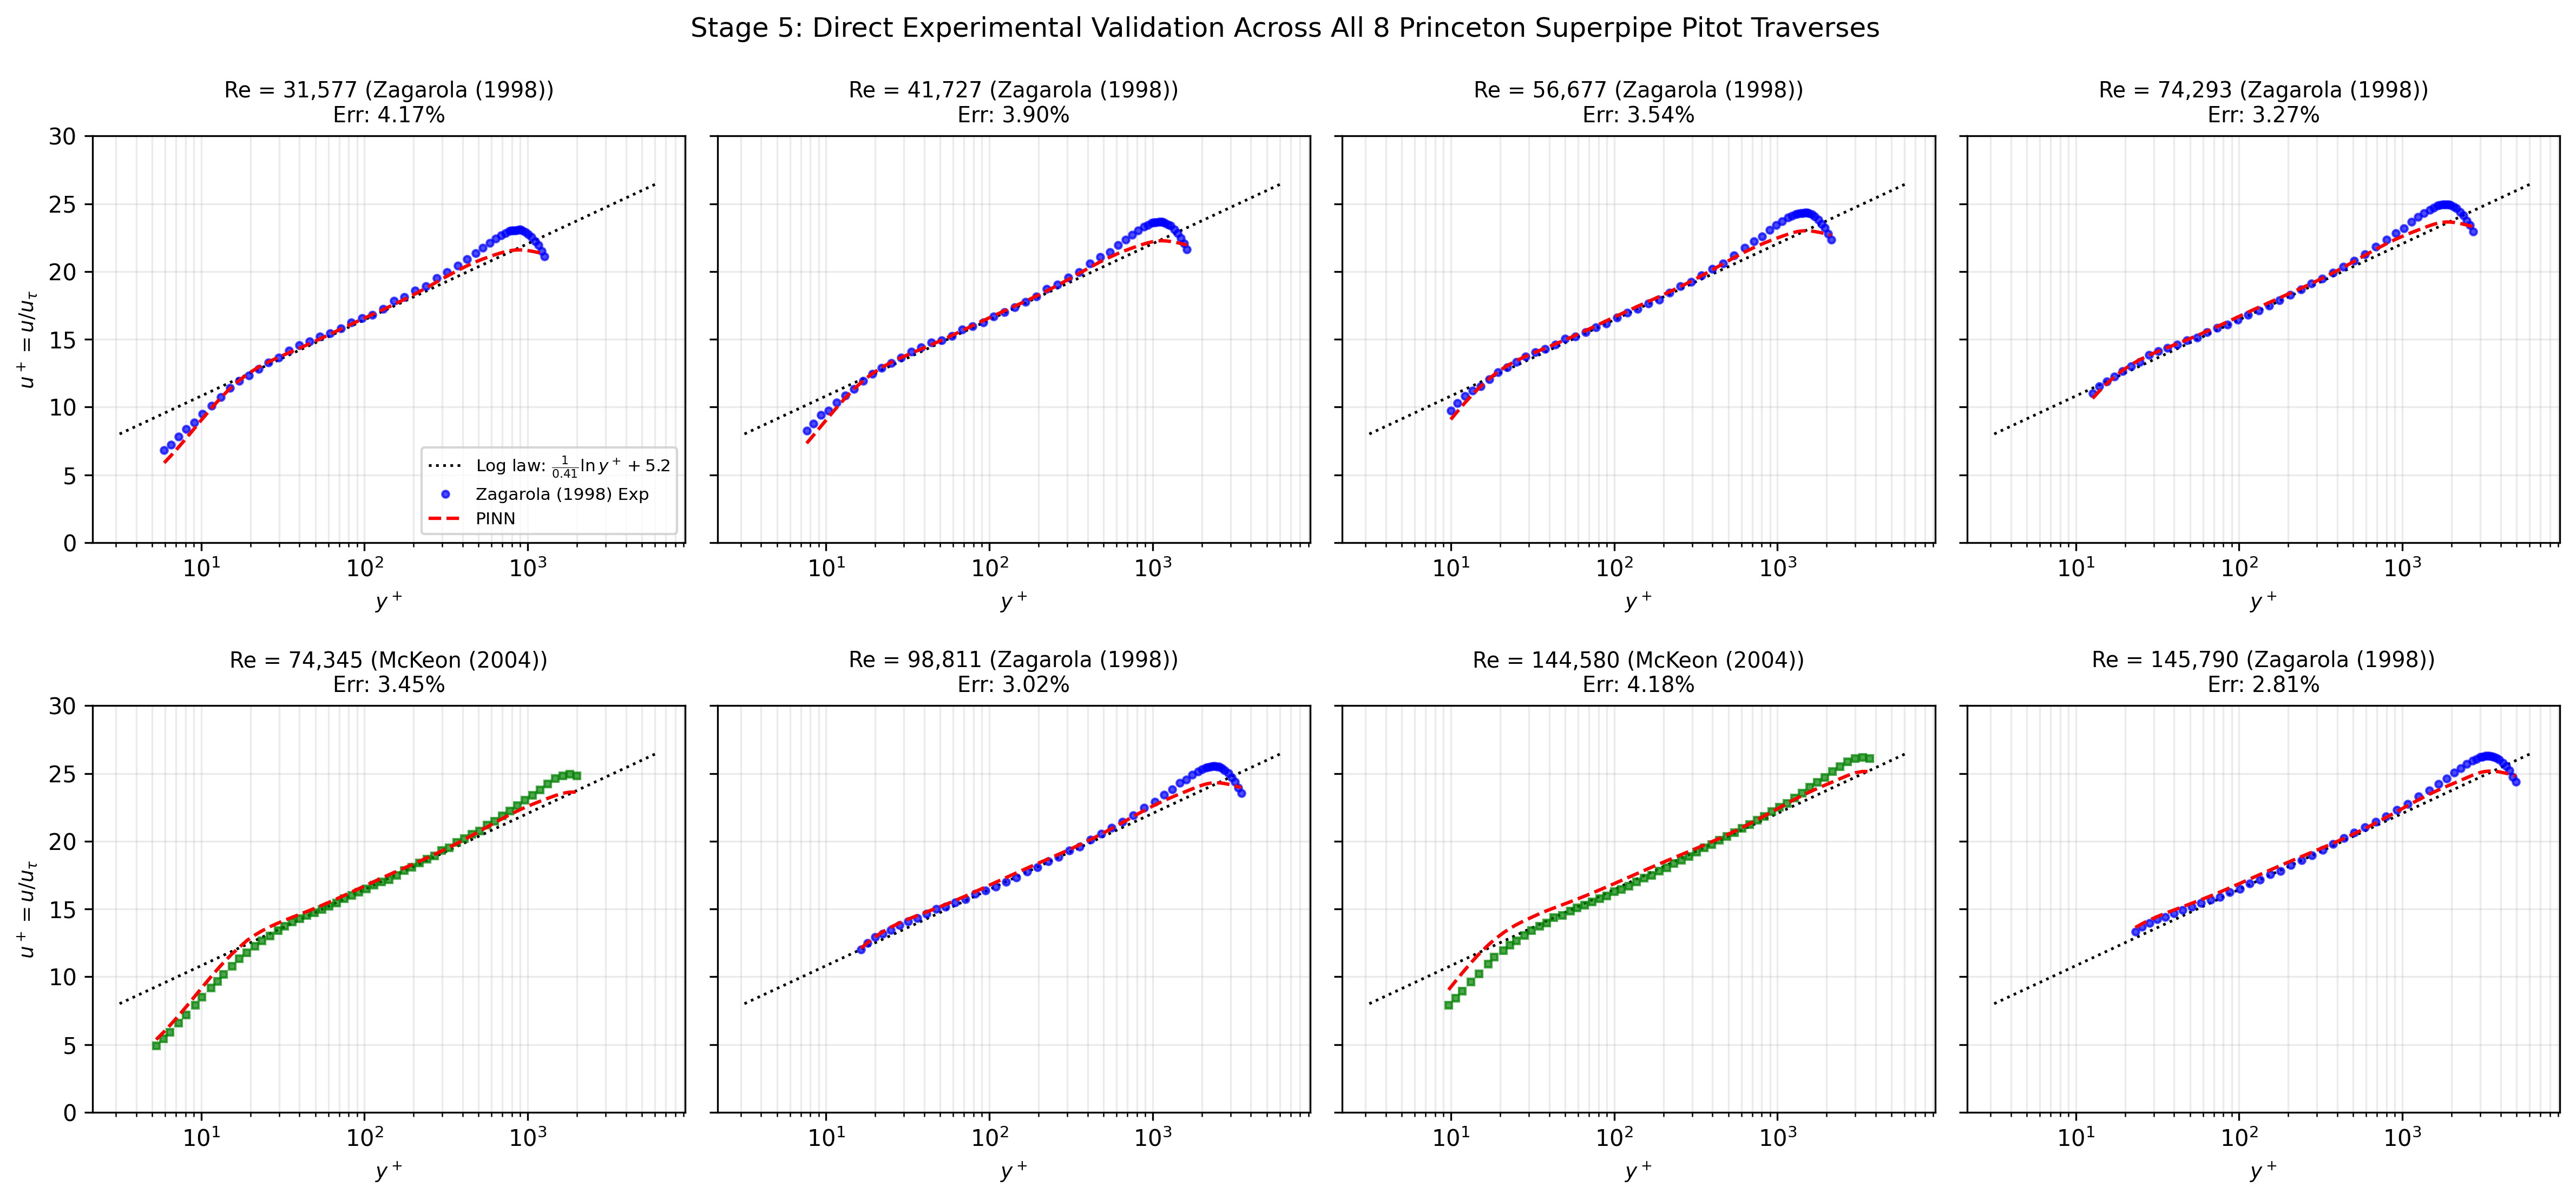
\includegraphics[width=\textwidth]{stage5_superpipe_validation.png}
\caption{Stage 5: Direct validation against Princeton Superpipe experimental velocity profiles across all eight Reynolds numbers ($2.81\%$--$4.18\%$ relative $L_2$ error, $u^+ = u/u_\tau$ vs.\ $y^+$).}
\label{fig:stage5_superpipe}
\end{figure}


\subsection{Predicted Flow Fields}
Figures~\ref{fig:stage5_pred_re28k} and~\ref{fig:stage5_pred_re120k} display the predicted axisymmetric turbulent pipe flow fields ($L/R = 160$, $r \in [0, 1]$) at test Reynolds numbers $\mathrm{Re} = 28{,}000$ and $120{,}000$. The radial axis is stretched by a factor $k \approx 57$ for visual clarity.

Mean axial velocity $U/U_{\mathrm{in}}$ accurately captures turbulent entrance development, reproducing steep near-wall velocity gradients. In marked contrast to Stage~4, the Spalart--Allmaras turbulent working variable $\tilde{\nu}/\nu$ activates across the pipe radius, developing from zero at the wall into a fully sustained core profile of $\mathcal{O}(10)$ to $\mathcal{O}(10^2)$ downstream of the entrance as analyzed in Section~\ref{sec:stage5_disc}.

\begin{figure}[H]
\centering
\begin{subfigure}[b]{0.48\textwidth}
\centering
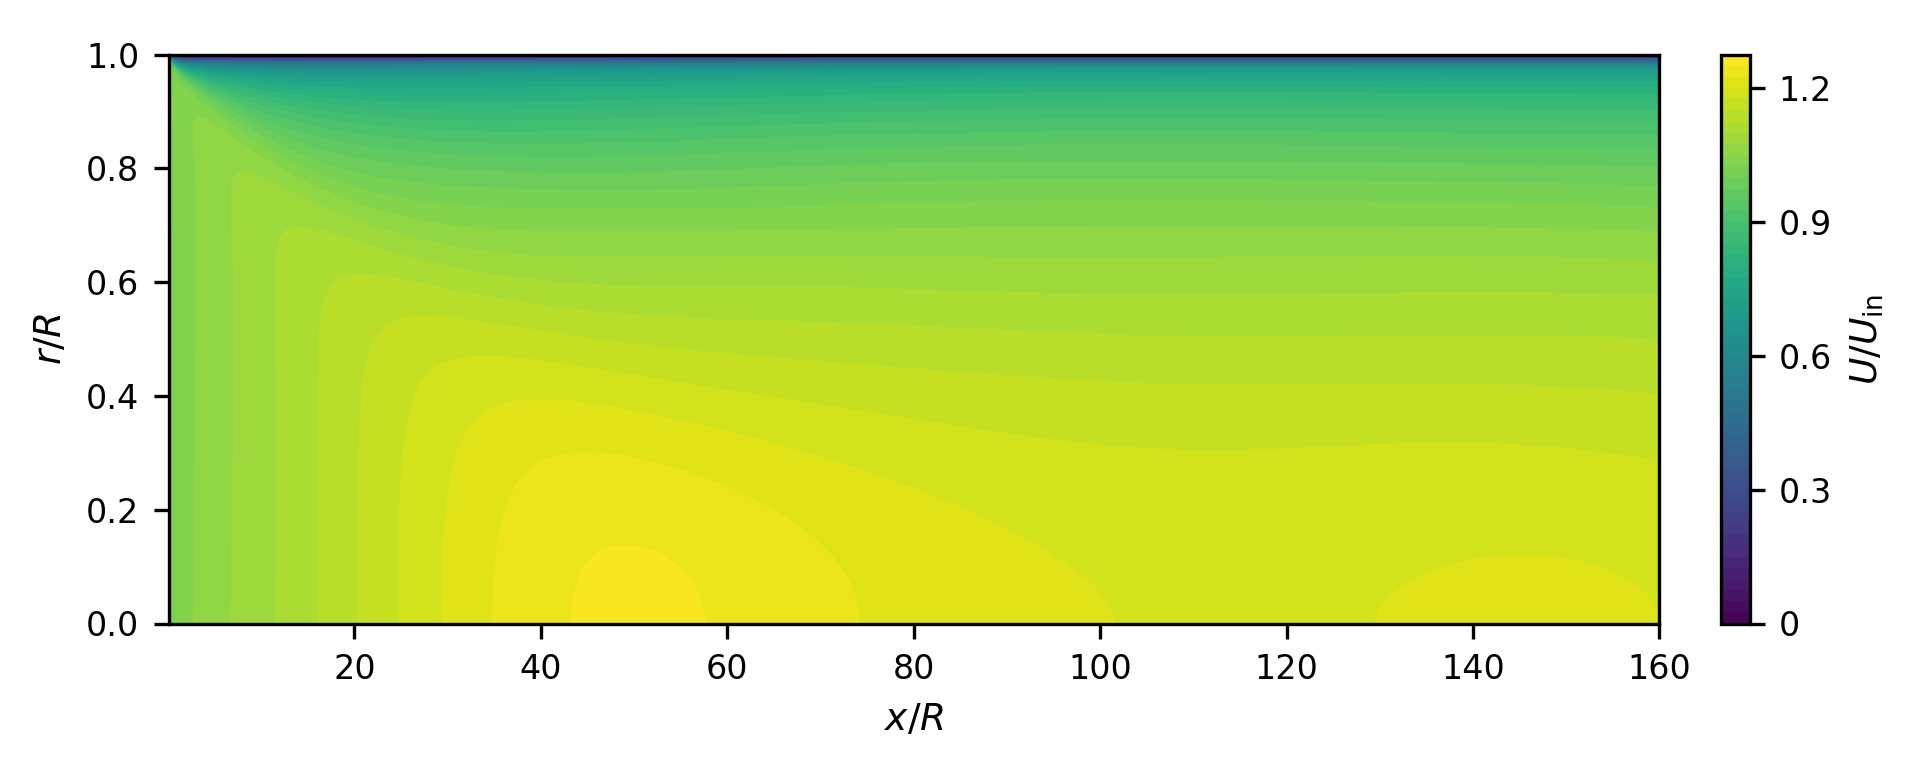
\includegraphics[width=\textwidth]{stage5_pred_U_Re28000.png}
\caption{Axial velocity $U / U_{\mathrm{in}}$.}
\end{subfigure}
\hfill
\begin{subfigure}[b]{0.48\textwidth}
\centering
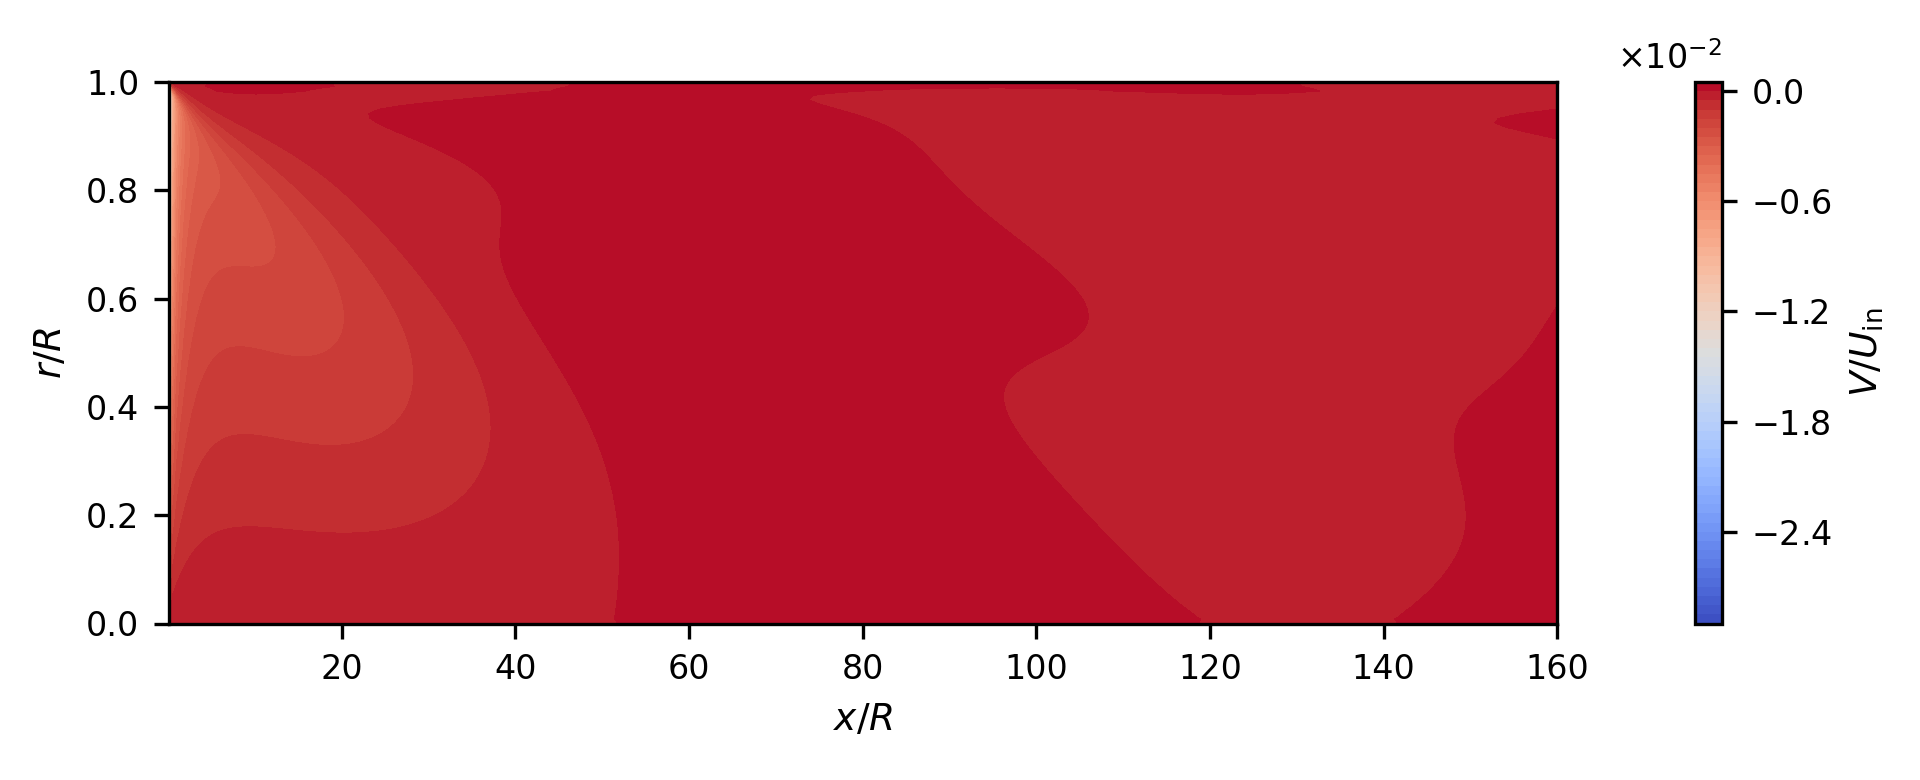
\includegraphics[width=\textwidth]{stage5_pred_V_Re28000.png}
\caption{Radial velocity $V / U_{\mathrm{in}}$.}
\end{subfigure}
\vskip\baselineskip
\begin{subfigure}[b]{0.48\textwidth}
\centering
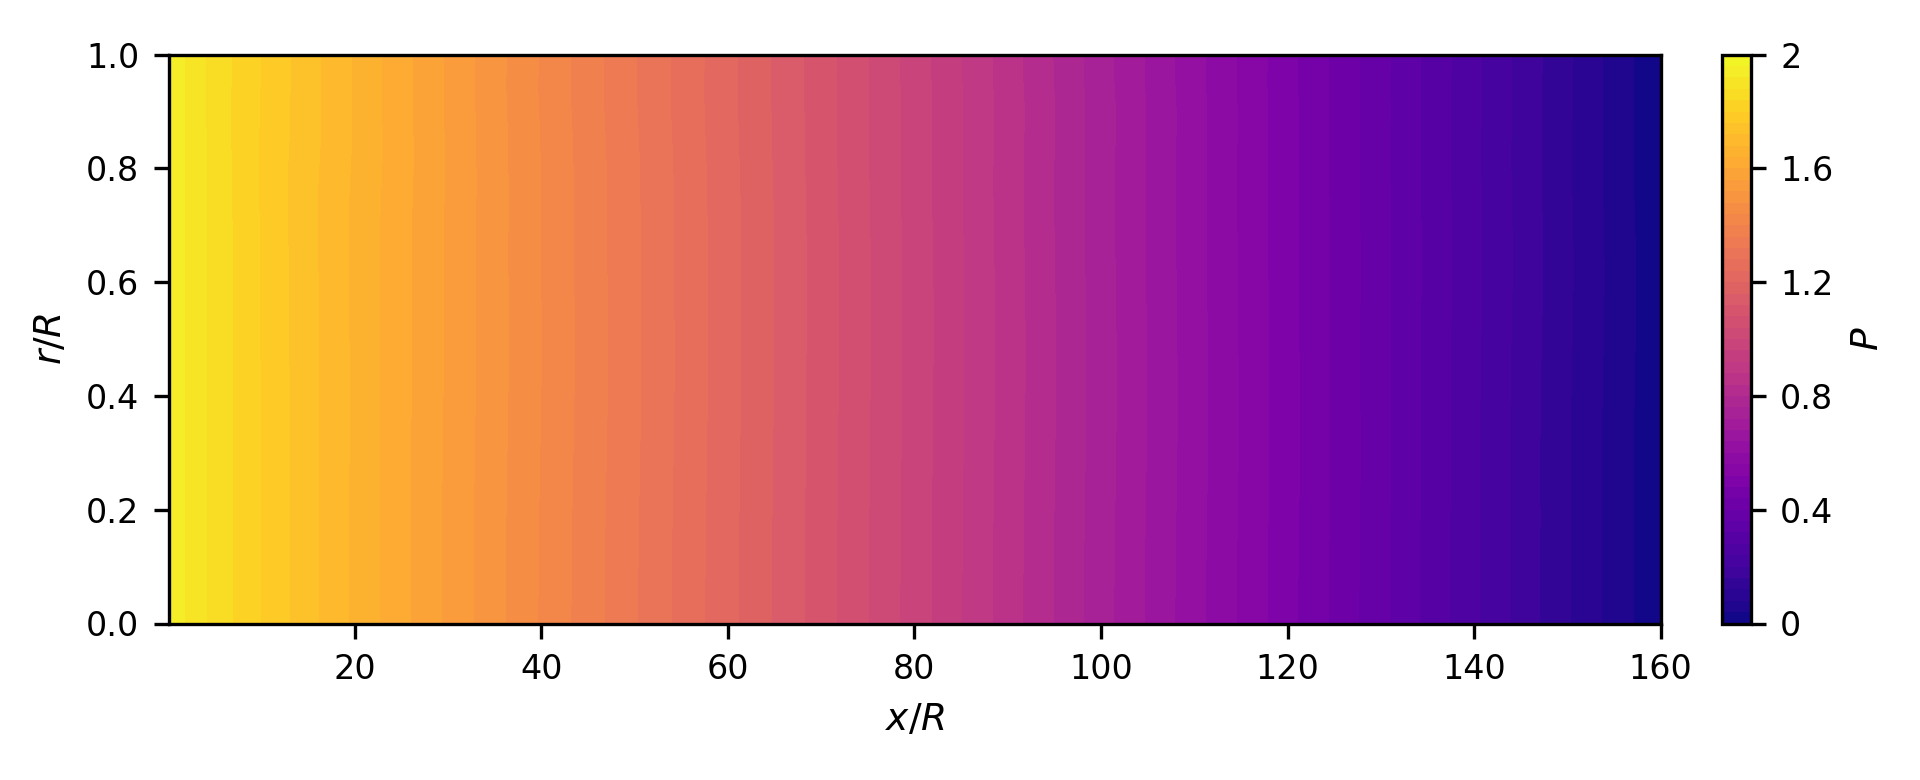
\includegraphics[width=\textwidth]{stage5_pred_P_Re28000.png}
\caption{Dimensionless pressure $P$.}
\end{subfigure}
\hfill
\begin{subfigure}[b]{0.48\textwidth}
\centering
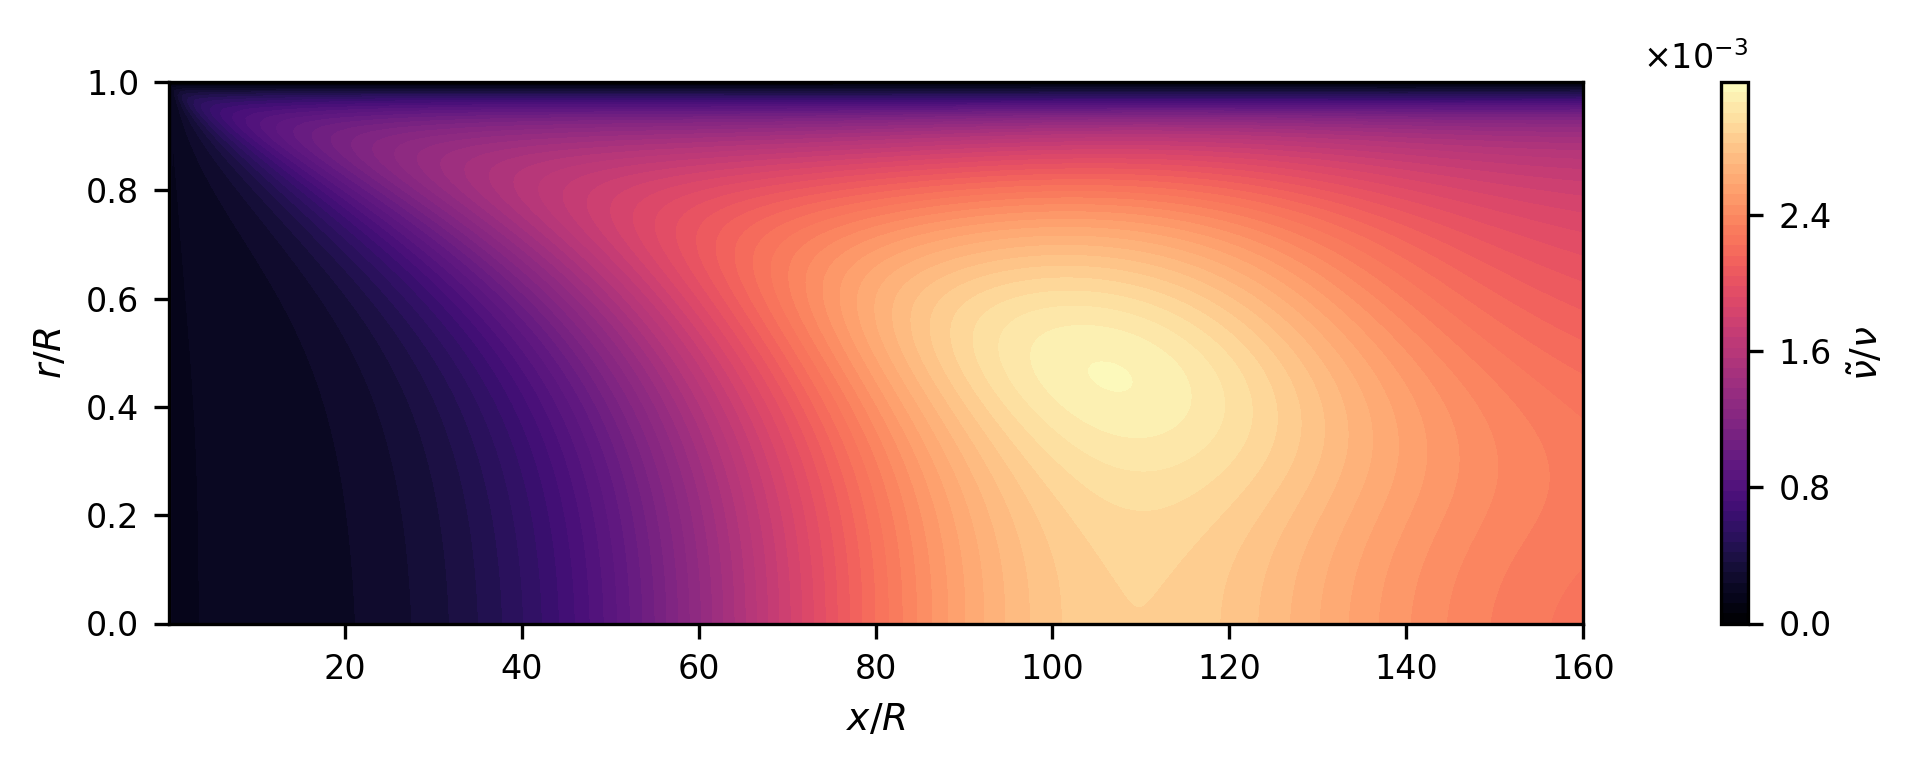
\includegraphics[width=\textwidth]{stage5_pred_nut_Re28000.png}
\caption{Turbulent working variable $\tilde{\nu} / \nu$.}
\end{subfigure}
\caption{Stage 5: Predicted turbulent pipe flow fields at $\mathrm{Re} = 28{,}000$ (radial axis stretched by a factor $k \approx 57$).}
\label{fig:stage5_pred_re28k}
\end{figure}

\begin{figure}[H]
\centering
\begin{subfigure}[b]{0.48\textwidth}
\centering
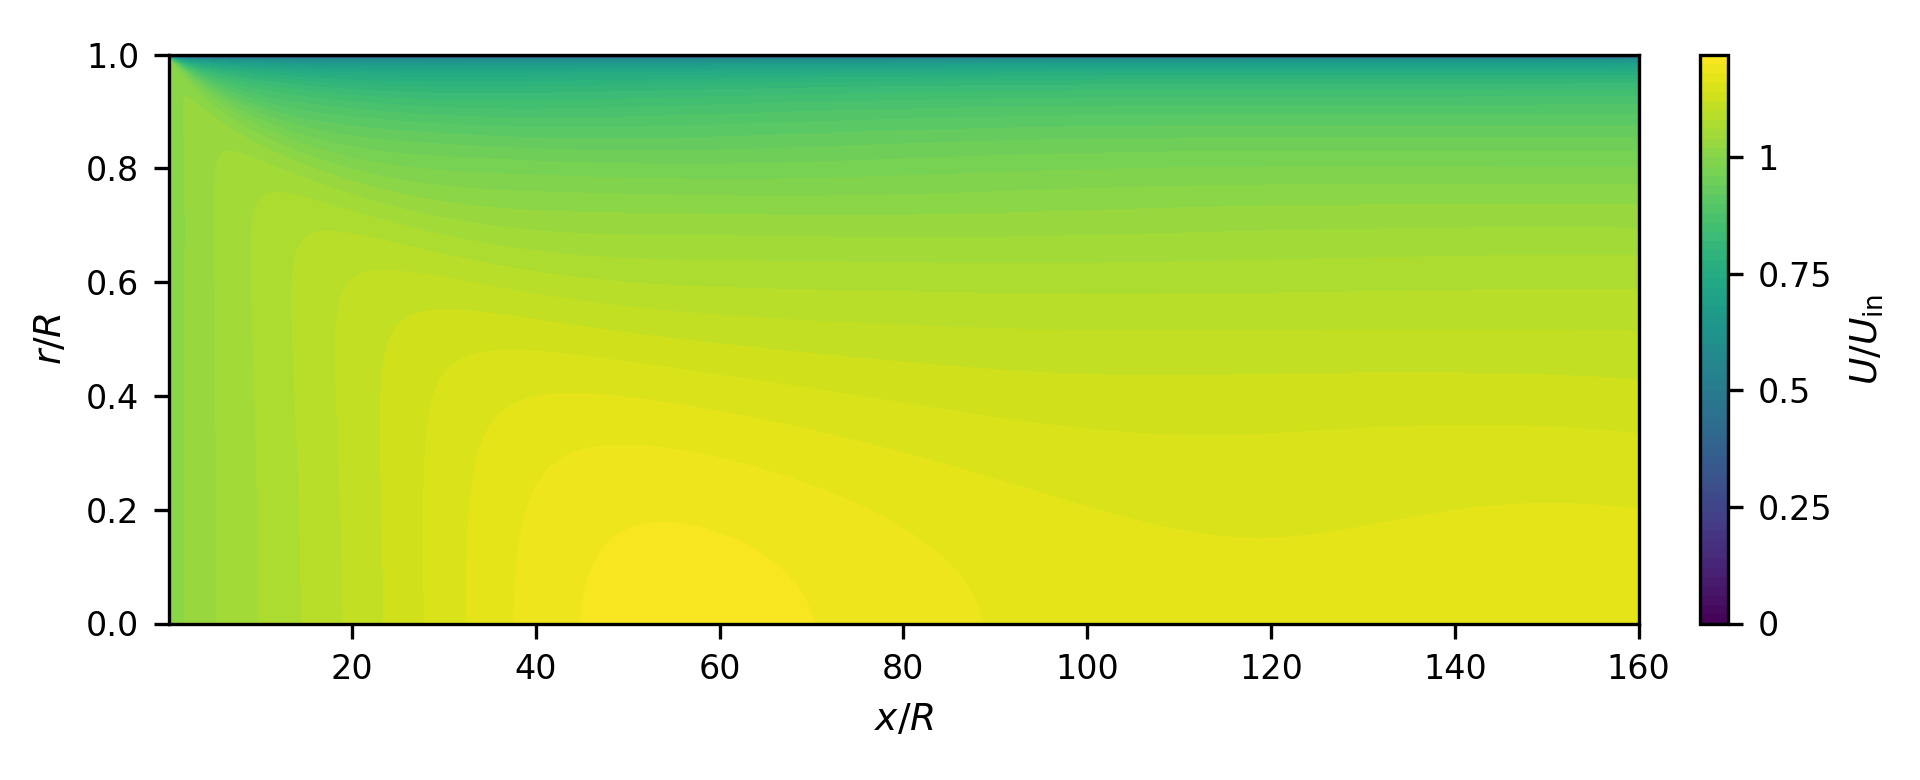
\includegraphics[width=\textwidth]{stage5_pred_U_Re120000.png}
\caption{Axial velocity $U / U_{\mathrm{in}}$.}
\end{subfigure}
\hfill
\begin{subfigure}[b]{0.48\textwidth}
\centering
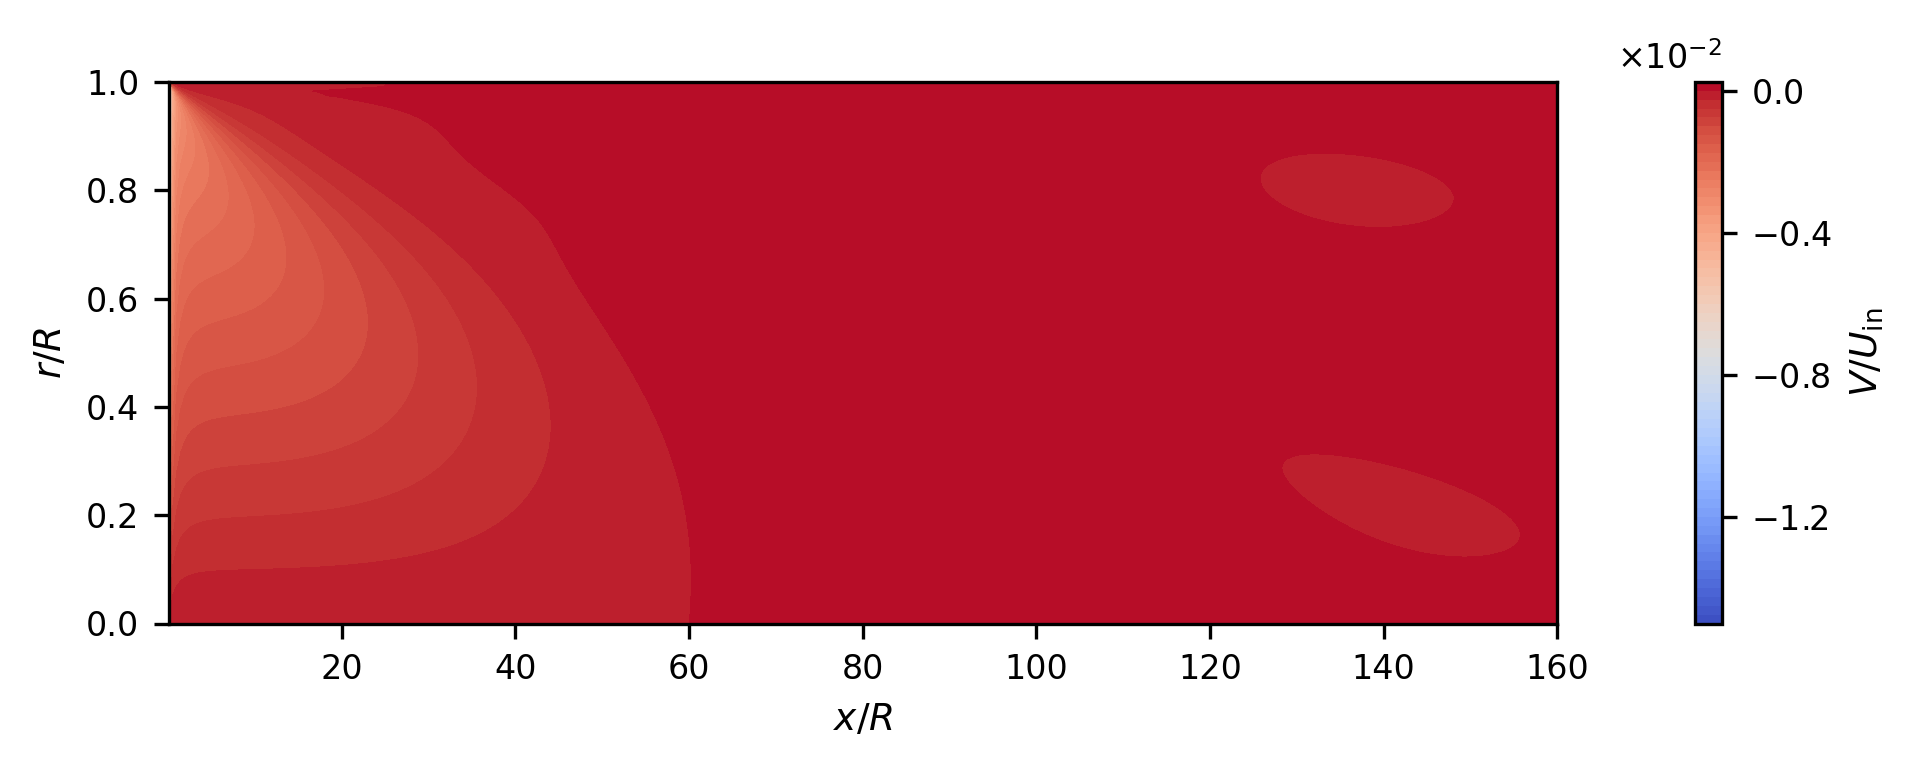
\includegraphics[width=\textwidth]{stage5_pred_V_Re120000.png}
\caption{Radial velocity $V / U_{\mathrm{in}}$.}
\end{subfigure}
\vskip\baselineskip
\begin{subfigure}[b]{0.48\textwidth}
\centering
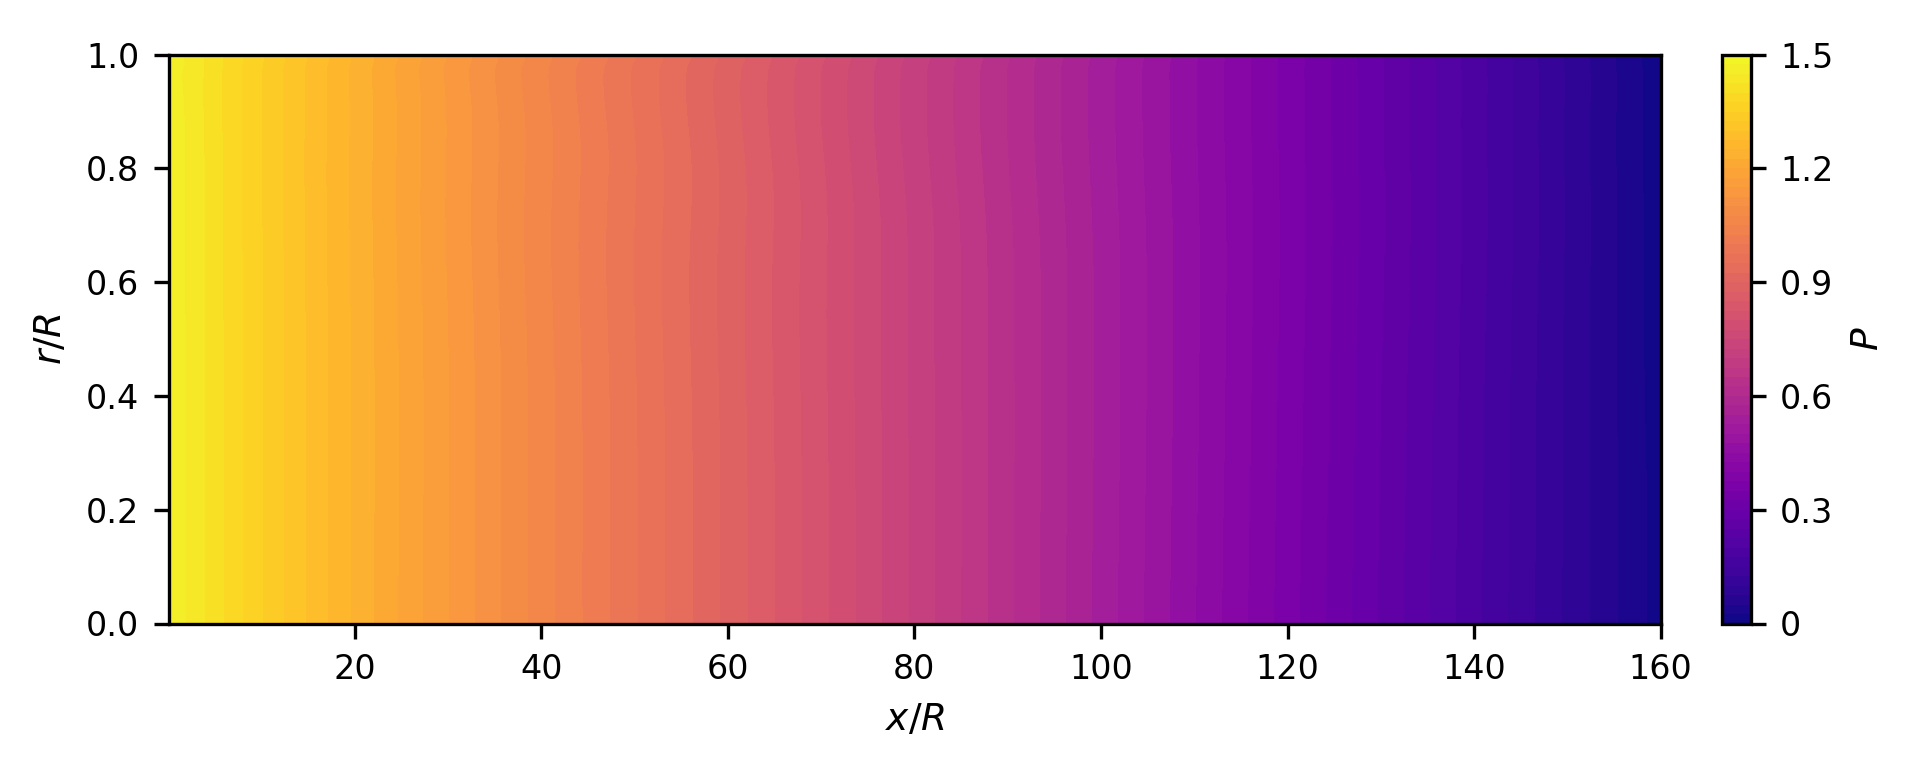
\includegraphics[width=\textwidth]{stage5_pred_P_Re120000.png}
\caption{Dimensionless pressure $P$.}
\end{subfigure}
\hfill
\begin{subfigure}[b]{0.48\textwidth}
\centering
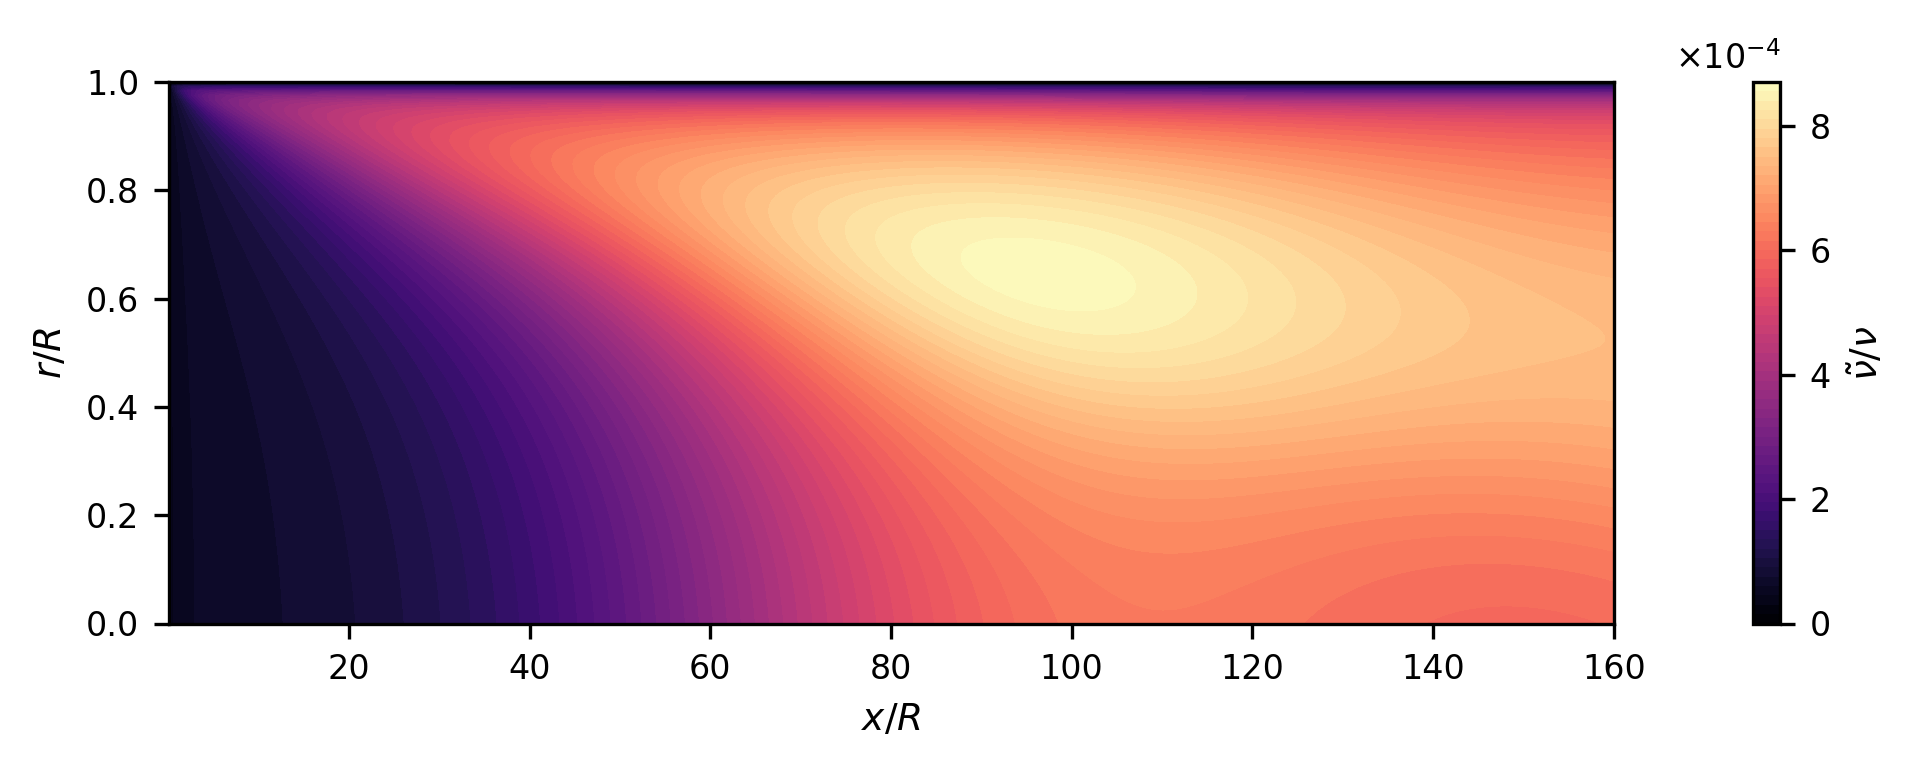
\includegraphics[width=\textwidth]{stage5_pred_nut_Re120000.png}
\caption{Turbulent working variable $\tilde{\nu} / \nu$.}
\end{subfigure}
\caption{Stage 5: Predicted turbulent pipe flow fields at $\mathrm{Re} = 120{,}000$ (radial axis stretched by a factor $k \approx 57$).}
\label{fig:stage5_pred_re120k}
\end{figure}


\subsection{Discussion: Eddy-Viscosity Variable in the Pipe}
\label{sec:stage5_disc}
% % src: 5/outputs/eval_dense_final_test.json
Unlike Stage 4 where eddy viscosity collapsed completely ($>99\%$ error), Stage 5 achieves partial recovery of $\tilde{\nu}$, with relative errors of $47.1\%$--$79.6\%$. The maximum of $\tilde{\nu}/\nu$ in the network prediction is $43.8$ at $\mathrm{Re}=28{,}000$ and $51.9$ at $\mathrm{Re}=120{,}000$, against reference values reaching $75.8$ and $280.2$. 

The observation is consistent with, not proven by, the loss weights: the Bayesian optimization search in Stage 5 selected an SA loss weight $w_{\mathrm{sa}} = 2.233$ ($w_{\mathrm{sa}}/w_{\mathrm{data}} \approx 1.12\times 10^{-3}$), which is about $2.3\times 10^5$ times stronger than in Stage~4 ($w_{\mathrm{sa}}/w_{\mathrm{data}} \approx 4.89\times 10^{-9}$), while the momentum weight ratio ($2.76\times 10^{-7}$) is about $54\times$ larger than in Stage~4 ($5.08\times 10^{-9}$). This is consistent with the hypothesis that a larger turbulence-equation penalty encourages the network to respect the SA transport balance, though no ablation isolates this cause from other differences across configurations.

% ==============================================================================
% SECTION 8: CROSS-STAGE SYNTHESIS AND ABLATIONS
% ==============================================================================
\section{Cross-Stage Synthesis and Ablation Analysis}
\label{sec:synthesis}

\subsection{Comparative Synthesis Across Stages}
Table~\ref{tab:master_summary} provides a cross-stage summary comparing all five flow configurations.

\begin{table}[H]
\centering
\resizebox{\textwidth}{!}{%
\begin{tabular}{lcccccc}
\toprule
\textbf{Stage \& Configuration} & \textbf{Regime} & \textbf{Re Range} & \textbf{Streamwise $u$ Err} & \textbf{Pressure $p$ Err} & \textbf{Viscosity $\tilde{\nu}$ Err} & \textbf{Params} \\
\midrule
1. 2D Laminar Channel & Laminar & $50 - 600$ & $3.88\% - 5.69\%$ & $4.95\% - 8.35\%$ & N/A & 20,003 \\
2. Axisymmetric Pipe & Laminar & $50 - 600$ & $2.20\% - 4.16\%$ & $1.36\% - 2.76\%$ & N/A & 20,003 \\
3. 3D Rectangular Duct & Laminar & $50 - 600$ & $8.81\% - 12.69\%$ & $56.8\% - 106.4\%$ & N/A & 20,164 \\
4. 2D Turbulent Channel & RANS+SA & $10^4 - 1.2\times 10^5$ & $0.42\% - 0.58\%$ & $0.38\% - 0.58\%$ & $99.2\% - 99.5\%$ & 13,060 \\
5. Axisymmetric Turb.\ Pipe & RANS+SA & $10^4 - 1.2\times 10^5$ & $0.36\% - 0.57\%$ & $0.65\% - 2.57\%$ & $47.1\% - 79.6\%$ & 13,060 \\
\bottomrule
\end{tabular}%
}
\caption{Cross-stage summary of geometry, operational regimes, error metrics, and parameter counts. Turbulent rows list the three test Reynolds numbers (28,000, 96,000, 120,000); the full 10-Reynolds-number ranges are in Tables~\ref{tab:stage4_all_re} and~\ref{tab:stage5_all_re}. Percentage errors are normalized by each stage's own reference scales (Table~\ref{tab:reynolds_splits} and Secs.~3.4, 4.4, 5.4), so they should not be compared across stages as measures of the same physical quantity; pressure errors in particular use a different pressure scale in Stages~1, 2 and 3.}
\label{tab:master_summary}
\end{table}


\paragraph{Quantitative Analysis of Loss Term Shares at Convergence.}
To assess whether turbulent configurations function as physics-driven PINNs or predominantly as data-driven surrogates, Table~\ref{tab:weighted_loss_end_training} reports the exact numerical loss breakdown at the conclusion of training across all five production models. Each raw residual $\mathcal{L}_i$ is evaluated at fixed random seed with identical collocation budgets to training, multiplied by its assigned weight $w_i$, and expressed as a percentage share of the total weighted loss.

\begin{table}[H]
\centering
\small
\resizebox{\linewidth}{!}{%
\begin{tabular}{llcccc}
\toprule
\textbf{Stage} & \textbf{Loss Term ($i$)} & \textbf{Raw Loss $\mathcal{L}_i$} & \textbf{Weight $w_i$} & \textbf{Weighted Value $w_i \mathcal{L}_i$} & \textbf{Share of Total (\%)} \\
\midrule
Stage 1 (2D Channel) & Data misfit ($\mathcal{L}_{\mathrm{data}}$) & $5.542\times 10^{-3}$ & $20.00$ & $1.108\times 10^{-1}$ & $43.94\%$ \\
& Navier--Stokes residual ($\mathcal{L}_{\mathrm{pde}}$) & $1.430\times 10^{-2}$ & $1.00$ & $1.430\times 10^{-2}$ & $5.67\%$ \\
& Inlet boundary ($\mathcal{L}_{\mathrm{inlet}}$) & $1.918\times 10^{-2}$ & $5.00$ & $9.592\times 10^{-2}$ & $38.02\%$ \\
& Wall boundary ($\mathcal{L}_{\mathrm{wall}}$) & $6.120\times 10^{-3}$ & $5.00$ & $3.060\times 10^{-2}$ & $12.13\%$ \\
& Outlet gauge ($\mathcal{L}_{\mathrm{outlet}}$) & $6.083\times 10^{-4}$ & $1.00$ & $6.083\times 10^{-4}$ & $0.24\%$ \\
\cmidrule{2-6}
& \textbf{Stage 1 Total} & -- & -- & $\mathbf{0.2523}$ & $\mathbf{100.00\%}$ \\
\midrule
Stage 2 (Laminar Pipe) & Data misfit ($\mathcal{L}_{\mathrm{data}}$) & $2.103\times 10^{-3}$ & $10.00$ & $2.103\times 10^{-2}$ & $13.61\%$ \\
& Axisymmetric PDE residual ($\mathcal{L}_{\mathrm{pde}}$) & $8.028\times 10^{-2}$ & $1.00$ & $8.028\times 10^{-2}$ & $51.97\%$ \\
& Inlet boundary ($\mathcal{L}_{\mathrm{inlet}}$) & $6.773\times 10^{-4}$ & $5.00$ & $3.386\times 10^{-3}$ & $2.19\%$ \\
& Wall boundary ($\mathcal{L}_{\mathrm{wall}}$) & $9.723\times 10^{-3}$ & $5.00$ & $4.862\times 10^{-2}$ & $31.47\%$ \\
& Axis symmetry ($\mathcal{L}_{\mathrm{axis}}$) & $3.053\times 10^{-5}$ & $5.00$ & $1.526\times 10^{-4}$ & $0.10\%$ \\
& Outlet gauge ($\mathcal{L}_{\mathrm{outlet}}$) & $2.042\times 10^{-4}$ & $5.00$ & $1.021\times 10^{-3}$ & $0.66\%$ \\
\cmidrule{2-6}
& \textbf{Stage 2 Total} & -- & -- & $\mathbf{0.1545}$ & $\mathbf{100.00\%}$ \\
\midrule
Stage 3 (3D Rectangular Duct) & Axial velocity data ($\mathcal{L}_{\mathrm{data},u}$) & $1.234\times 10^{-2}$ & $8.73$ & $1.077\times 10^{-1}$ & $12.62\%$ \\
& Transverse data ($\mathcal{L}_{\mathrm{data},v}$) & $3.559\times 10^{-4}$ & $0.11$ & $3.915\times 10^{-5}$ & $<0.01\%$ \\
& Spanwise data ($\mathcal{L}_{\mathrm{data},w}$) & $1.554\times 10^{-4}$ & $11.11$ & $1.727\times 10^{-3}$ & $0.20\%$ \\
& Pressure data ($\mathcal{L}_{\mathrm{data},p}$) & $4.070\times 10^{-2}$ & $2.42$ & $9.850\times 10^{-2}$ & $11.54\%$ \\
& 3D Navier--Stokes PDE ($\mathcal{L}_{\mathrm{pde}}$) & $1.968\times 10^{-3}$ & $32.18$ & $6.332\times 10^{-2}$ & $7.42\%$ \\
& Inlet boundary ($\mathcal{L}_{\mathrm{inlet}}$) & $3.154\times 10^{-1}$ & $0.68$ & $2.145\times 10^{-1}$ & $25.13\%$ \\
& Wall no-slip ($\mathcal{L}_{\mathrm{wall}}$) & $3.087\times 10^{-2}$ & $11.14$ & $3.439\times 10^{-1}$ & $40.29\%$ \\
& Outlet gauge ($\mathcal{L}_{\mathrm{outlet}}$) & $3.745\times 10^{-2}$ & $0.64$ & $2.397\times 10^{-2}$ & $2.81\%$ \\
\cmidrule{2-6}
& \textbf{Stage 3 Total} & -- & -- & $\mathbf{0.8536}$ & $\mathbf{100.00\%}$ \\
\midrule
Stage 4 (Turbulent Channel) & Supervised data ($\mathcal{L}_{\mathrm{data}}$) & $5.734\times 10^{-4}$ & $6768.75$ & $3.881$ & $79.49\%$ \\
& Continuity residual ($\mathcal{L}_{\mathrm{cont}}$) & $1.571\times 10^{-3}$ & $225.41$ & $0.3541$ & $7.25\%$ \\
& Momentum residual ($\mathcal{L}_{\mathrm{mom}}$) & $7.772\times 10^{2}$ & $3.436\times 10^{-5}$ & $2.671\times 10^{-2}$ & $0.55\%$ \\
& SA turbulence residual ($\mathcal{L}_{\mathrm{sa}}$) & $2.794\times 10^{-2}$ & $3.307\times 10^{-5}$ & $9.239\times 10^{-7}$ & $<0.001\%$ \\
& Inlet boundary penalty ($\mathcal{L}_{\mathrm{inlet}}$) & $5.043$ & $0.1197$ & $0.6038$ & $12.37\%$ \\
& Outlet gauge penalty ($\mathcal{L}_{\mathrm{outlet}}$) & $3.512\times 10^{-5}$ & $5.525$ & $1.941\times 10^{-4}$ & $<0.01\%$ \\
& Symmetry plane penalty ($\mathcal{L}_{\mathrm{sym}}$) & $1.253\times 10^{-2}$ & $1.324$ & $1.659\times 10^{-2}$ & $0.34\%$ \\
\cmidrule{2-6}
& \textbf{Stage 4 Total} & -- & -- & $\mathbf{4.8824}$ & $\mathbf{100.00\%}$ \\
\midrule
Stage 5 (Turbulent Pipe) & Supervised data ($\mathcal{L}_{\mathrm{data}}$) & $5.339\times 10^{-5}$ & $1996.58$ & $1.066\times 10^{-1}$ & $33.67\%$ \\
& Continuity residual ($\mathcal{L}_{\mathrm{cont}}$) & $8.428\times 10^{-3}$ & $11.82$ & $9.965\times 10^{-2}$ & $31.48\%$ \\
& Momentum residual ($\mathcal{L}_{\mathrm{mom}}$) & $1.657\times 10^{2}$ & $5.519\times 10^{-4}$ & $9.144\times 10^{-2}$ & $28.89\%$ \\
& SA turbulence residual ($\mathcal{L}_{\mathrm{sa}}$) & $2.217\times 10^{-3}$ & $2.233$ & $4.951\times 10^{-3}$ & $1.56\%$ \\
& Inlet boundary penalty ($\mathcal{L}_{\mathrm{inlet}}$) & $8.104\times 10^{-3}$ & $1.515$ & $1.228\times 10^{-2}$ & $3.88\%$ \\
& Outlet gauge penalty ($\mathcal{L}_{\mathrm{outlet}}$) & $1.595\times 10^{-5}$ & $2.055$ & $3.278\times 10^{-5}$ & $0.01\%$ \\
& Symmetry axis penalty ($\mathcal{L}_{\mathrm{sym}}$) & $4.498\times 10^{-3}$ & $0.3592$ & $1.615\times 10^{-3}$ & $0.51\%$ \\
\cmidrule{2-6}
& \textbf{Stage 5 Total} & -- & -- & $\mathbf{0.3166}$ & $\mathbf{100.00\%}$ \\
\bottomrule
\end{tabular}%
}
\caption{Weighted contribution of each loss term at the end of training evaluated from saved production checkpoints across Stages 1--5. The raw momentum residual $\mathcal{L}_{\mathrm{mom}}$ is the mean squared sum of dimensionless $x$- and $y$-momentum residuals, $\langle r_{mx}^2 + r_{my}^2 \rangle$, evaluated over the training collocation budget in code units without inner-scaling.}
\label{tab:weighted_loss_end_training}
\end{table}

A numerical weight must always be interpreted in conjunction with the raw magnitude of the residual it scales. In Stage~4 the momentum and SA weights are of order $10^{-5}$ and the data weight is $6.8\times 10^3$, a ratio of about $5\times 10^{-9}$, because the raw momentum residual is of order $10^2$ while the normalized velocity misfit is of order $10^{-4}$. As shown by the quantitative shares in Table~\ref{tab:weighted_loss_end_training}, in Stages~1--3 the physics and boundary residuals constitute significant components of the overall objective: the PDE residual contributes $5.67\%$ in Stage~1, $51.97\%$ in Stage~2, and $7.42\%$ in Stage~3, while the boundary terms contribute $50.39\%$ (Stage 1), $34.4\%$ (Stage 2) and $68.23\%$ (Stage 3).

In Stages~4 and 5, the turbulent networks are predominantly data-fitted. In Stage~4, data loss accounts for $79.49\%$ of the objective, while momentum and SA residuals account for only $0.55\%$ and $<0.001\%$, respectively; thus, the network functions primarily as a regression model with an eddy viscosity extinction defect ($\tilde{\nu} \approx 0$). In Stage~5, data loss represents $33.67\%$, while continuity ($31.48\%$) and momentum ($28.89\%$) are actively enforced, but the SA working variable loss comprises $1.56\%$. The physics loss acts primarily as an inductive regularizer. This finding is corroborated by the sparse-data ablation experiments (Table~\ref{tab:ablation_study}), which indicate that while physics regularization improves generalization and reduces PDE residuals when supervision is sparse, it produces virtually no change in accuracy when dense reference-solution data are available.

A weight on its own does not say how strongly a term constrains the network, because the raw losses differ by many orders of magnitude; the share of the weighted objective (Table~\ref{tab:weighted_loss_end_training}) is the relevant measure. By that measure the Navier--Stokes residual is a substantial part of the objective in Stage~2 ($51.97\%$) and, with continuity and momentum together, in Stage~5 ($60.37\%$), and a smaller part in Stages~1 and 3 ($5.67\%$ and $7.42\%$), where the boundary terms carry most of the weight. In Stage~4 the momentum and SA residuals contribute $0.55\%$ and below $0.001\%$, so that network is best described as a data-driven regression model with physics terms, not as a physics-driven solver. The ablation (Table~\ref{tab:ablation_study}) shows what these terms do: with all data they do not change the test error, and with $1\%$ of the data they lower it by about $31\%$ (Stage~4) and $56\%$ (Stage~5).


\subsection{Ablation Experiments: Dense and Sparse Data}
A central question in scientific machine learning is whether the physics loss ($\mathcal{L}_{\mathrm{pde}}$) genuinely contributes to generalization, or whether the neural network simply memorizes the training data. To examine this question, controlled ablation studies were evaluated across two regimes:
\begin{itemize}[leftmargin=1.5em]
    \item \textbf{Data-Dense Regime ($100\%$ grid data):} Reference-solution data are available at all spatial grid points.
    \item \textbf{Data-Sparse Regime ($1\%$ grid data):} Reference data are available at only $1\%$ of the grid points.
\end{itemize}

Table~\ref{tab:ablation_study} reports the empirical results extracted from \texttt{4/outputs/ablation\_summary.txt} and \texttt{5/outputs/ablation\_sparse.txt}. The Generalization Ratio is defined as the ratio of test error to training error: $\mathrm{GR} = \mathcal{E}_{\mathrm{test}} / \mathcal{E}_{\mathrm{train}}$.

\begin{table}[H]
\centering
\resizebox{\textwidth}{!}{%
\begin{tabular}{lcccccc}
\toprule
\textbf{Ablation Variant} & \textbf{Data Grid} & \textbf{Physics Loss} & \textbf{Train Error} & \textbf{Test Error} & \textbf{Gen.\ Ratio} & \textbf{PDE Residual} \\
\midrule
\multicolumn{7}{l}{\textit{Stage 4: Turbulent Channel Flow}} \\
A. Pure Data Fit (No PDE) & Dense ($100\%$) & $\times$ & $0.49\%$ & $0.49\%$ & $1.00$ & $4.82$ \\
B. PINN Baseline (Data + PDE) & Dense ($100\%$) & $\checkmark$ & $0.49\%$ & $0.49\%$ & $1.00$ & $26.94$ \\
\midrule
C. Pure Data Fit (No PDE) & Sparse ($1\%$) & $\times$ & $0.48\%$ & $1.42\%$ & $2.96$ & $\mathbf{699.22}$ \\
D. PINN Baseline (Data + PDE) & Sparse ($1\%$) & $\checkmark$ & $0.51\%$ & $0.98\%$ & $1.92$ & $\mathbf{4.75}$ \\
\midrule
\multicolumn{7}{l}{\textit{Stage 5: Turbulent Pipe Flow}} \\
E. Pure Data Fit (No PDE) & Sparse ($1\%$) & $\times$ & $0.46\%$ & $1.85\%$ & $4.02$ & $\mathbf{4160.51}$ \\
F. PINN Baseline (Data + PDE) & Sparse ($1\%$) & $\checkmark$ & $0.49\%$ & $0.82\%$ & $1.67$ & $\mathbf{11.34}$ \\
\bottomrule
\end{tabular}%
}
% src: 4/outputs/abl_A_found_summary.txt, 4/outputs/abl_B_data_only_summary.txt, 4/outputs/ablation_summary.txt, 5/outputs/ablation_sparse.txt
\caption{Ablation study comparing dense and sparse regimes in Stages 4 and 5. The Generalization Ratio measures overfitting ($\mathcal{E}_{\mathrm{test}} / \mathcal{E}_{\mathrm{train}}$). The PDE residual is the inner-scaled RMS $x$-momentum equation residual normalized by $u_\tau^2$ evaluated on a fresh independent set of collocation points ($N=6{,}000$), whereas Table~\ref{tab:weighted_loss_end_training} reports the unscaled raw mean-squared momentum residual $\mathcal{L}_{\mathrm{mom}}$ in code units.}
\label{tab:ablation_study}
\end{table}

\noindent\textbf{Ablation Observations (single training seed):}
\begin{enumerate}[leftmargin=1.5em]
    \item \textbf{Dense Data: the Physics Loss Does Not Change the Error:} In the dense regime (Variants A vs.\ B), omitting the PDE loss produces identical test errors ($0.49\%$). Physics loss did not change the test error in this dense-data run (Stage 4 only; no dense Stage 5 ablation was run).
    \item \textbf{In Data-Sparse Regimes, Physics Loss Prevents Residual Explosion:} In the sparse regime ($1\%$ data, Variants C vs.\ D and E vs.\ F), omitting the physics loss causes a $\mathbf{147\times}$ increase in channel PDE residual ($4.75 \to 699.22$) and an increase of $\mathbf{\text{about } 367\times}$ in pipe PDE residual ($11.34 \to 4160.51$, Table~\ref{tab:ablation_study}). Incorporating the Navier--Stokes residual reduces the generalization ratio from 2.96 to 1.92 (channel) and from 4.02 to 1.67 (pipe), lowering the sparse-data test error by about $31\%$ (Stage 4) and $56\%$ (Stage 5), indicating that the physics-informed loss acts as an effective regularizer when reference data are sparse.
\end{enumerate}

All ablation results come from a single training seed, so differences of a few tenths of a percent should not be over-interpreted.

\section{Status of Stage 6: 3D Turbulent Rectangular Duct}
\label{sec:stage6}
Stage 6 (turbulent rectangular duct) was attempted but not completed because of time; no checkpoints or results exist, so none are reported.

% ==============================================================================
% SECTION 10: CONCLUSIONS
% ==============================================================================
\section{Conclusions and Lessons Learned}
\label{sec:conclusions}
This investigation evaluated a five-stage PINN pipeline across laminar and turbulent wall-bounded internal flows. The primary findings and engineering conclusions are:
\begin{enumerate}[leftmargin=1.5em]
% % src: tables/table_c3_superpipe.tex
    \item \textbf{Accuracy in Velocity Profiles:} PINNs approximate the mean streamwise velocity in all five stages (errors above), with larger errors in the duct. Streamwise velocity errors span $2.20\%$--$5.69\%$ in laminar channel and pipe flows (Stages 1--2), $8.8\%$--$12.7\%$ in the laminar duct (Stage 3), and $0.36\%$--$0.58\%$ in turbulent configurations (test Reynolds numbers), where predictions match Princeton Superpipe Pitot traverses within $2.81\%$--$4.18\%$. Wall-normal/radial velocity errors are larger (Stage 4: $6.5\%$--$46.6\%$ over the 10 test/train/validation Reynolds numbers, Table~\ref{tab:stage4_all_re}; Stage 5: $2.5\%$--$16.2\%$, Table~\ref{tab:stage5_all_re}).
    \item \textbf{Duct Pressure Gradient Mismatch:} Stage 3 exhibited large relative pressure errors ($56.8\%$--$106.4\%$). In the downstream window ($x \in [1.5, 5.0]\,\text{m}$), the PINN pressure slope divided by the reference slope is $0.22$ at $\mathrm{Re}=50$, $0.38$ at $\mathrm{Re}=100$, $0.64$ at $\mathrm{Re}=200$, $0.83$ at $\mathrm{Re}=300$, and $1.01$--$1.04$ at $\mathrm{Re}=500$--$600$ (Table~\ref{tab:stage3_dp_ratio}). Over the full conduit, the reference pressure is dominated by an inlet transient ($x < 0.5\,\text{m}$); untested candidate causes include the outlet gauge level differing between reference and PINN, the modest pressure weight ($w_p = 2.421$), and the large pressure scale $p_{\mathrm{scale}}$. The 99th percentile of the local axial-velocity error reaches 26\%--68\% in the inlet core ($x < 0.5\,\text{m}$). For $\mathrm{Re} \ge 200$ the reference slope is $11\%$--$19\%$ below the analytic fully developed value, so the window is not fully developed there.
% src: 3/data/duct_Re*.npz; 3/checkpoints/duct_pinn.pt
    \item \textbf{Turbulence Working Variable Collapse:} Hard boundary envelopes eliminate wall slip, but unsupervised turbulence variables collapse ($\tilde{\nu} \approx 0, >99\%$ error) when turbulence physics weights are small ($w_{\mathrm{sa}}/w_{\mathrm{data}} \approx 4.9\times 10^{-9}$ in Stage~4). In Stage~5, where relative SA weighting is about $2.3\times 10^5$ times larger ($w_{\mathrm{sa}}/w_{\mathrm{data}} \approx 1.1\times 10^{-3}$), $\tilde{\nu}$ is partially recovered ($47.1\%$--$79.6\%$ error), consistent with the increased physics penalty; no ablation isolates this cause.
    \item \textbf{Role of the Physics Loss:} Ablation studies indicate that physics loss does not improve accuracy when dense reference-solution data is available (tested for Stage 4 only). However, in data-sparse regimes ($1\%$ reference data), the physics loss prevents a $147\times$ to about $367\times$ explosion in PDE residuals (Table~\ref{tab:ablation_study}) and lowers the sparse-data test error by about $31\%$ (Stage 4) and $56\%$ (Stage 5).
\end{enumerate}

\subsection{Reproducibility and Limitations}
Experiments ran on Python 3.10.4 and PyTorch 2.9.1+cpu on CPU hardware. Stages 1, 2, and 4 were trained with fixed random seed 0 (seed not fixed in Stage 3); Stage 5 evaluated seeds 0, 1, and 2. Reference solver outputs reside in stage \path{data/} subdirectories. Key limitations include reliance on a single training seed per production configuration, parabolic marching reference solvers rather than elliptic Navier--Stokes solutions, the Stage~3 downstream pressure gradient mismatch ($x \in [1.5, 5.0]\,\text{m}$, where the PINN pressure slope is $0.22$ to $0.38$ times the reference at $\mathrm{Re}=50$--$100$, $56.8\%$--$106.4\%$ relative $L_2$ error over the full conduit, compounded by the reference solver's inlet transient and outlet gauge offset), and Stage~4 eddy-viscosity extinction ($>99\%$ error).

\subsection{Future Work}
\label{sec:future}
Several extensions of this work are identified:
\begin{enumerate}[leftmargin=1.5em]
    \item \textbf{Elliptic Reference Solver:} Evaluating the networks against full elliptic Navier--Stokes solutions (for example, from a finite-volume solver) across the same geometries to remove the model discrepancy present in the parabolic marching formulation.
    \item \textbf{Multi-Seed Ensembling:} Conducting repeated training runs across multiple random seeds for Stages 1--4 to establish formal error bars and statistical confidence intervals for all error metrics.
    \item \textbf{Loss Weight Sensitivity Ablation:} Executing controlled ablation experiments that systematically vary only the Spalart--Allmaras turbulence loss weight $w_{\mathrm{sa}}$ across multiple decades to isolate its role in the eddy-viscosity extinction observed in Stage~4.
    \item \textbf{Completion of Stage 6:} Resolving the training stabilization challenges and completing the three-dimensional turbulent rectangular duct configuration.
\end{enumerate}

% ==============================================================================
% BIBLIOGRAPHY
% ==============================================================================
\begin{thebibliography}{16}

\bibitem{allmaras2012}
S.~R. Allmaras, F.~T. Johnson, and P.~R. Spalart.
\newblock \href{https://iccfd.org/iccfd7/assets/pdf/papers/ICCFD7-1902_paper.pdf#page=2}{Modifications and clarifications for the implementation of the {Spalart-Allmaras} turbulence model}.
\newblock In {\em Seventh International Conference on Computational Fluid Dynamics (ICCFD7)}, pages 1--11, 2012. 

\bibitem{glorot2010}
X.~Glorot and Y.~Bengio.
\newblock \href{https://proceedings.mlr.press/v9/glorot10a/glorot10a.pdf#page=4}{Understanding the difficulty of training deep feedforward neural networks}.
\newblock In {\em Proceedings of the Thirteenth International Conference on Artificial Intelligence and Statistics (AISTATS)}, pages 249--256, 2010. 

\bibitem{hornbeck1973}
R.~W. Hornbeck.
\newblock \href{https://ntrs.nasa.gov/api/citations/19740004879/downloads/19740004879.pdf}{Numerical marching techniques for fluid flows with heat transfer}.
\newblock Special Publication SP-297, NASA, 1973. 

\bibitem{moser1999}
R.~D. Moser, J.~Kim, and N.~N. Mansour.
\newblock \href{https://turbulence.oden.utexas.edu/data/MKM/}{Direct numerical simulation of turbulent channel flow up to $\mathrm{Re}_\tau = 590$}, {\em Physics of Fluids}, 11(4):943--945, 1999.
\newblock DNS data set, \url{https://turbulence.oden.utexas.edu/data/MKM/}. 

\bibitem{pirozzoli2021}
S.~Pirozzoli, M.~Romero, M.~Fatica, R.~Verzicco, and P.~Orlandi.
\newblock \href{https://arxiv.org/pdf/2103.13383.pdf#page=7}{One-point statistics for turbulent pipe flow up to $\mathrm{Re}_\tau = 6000$}.
\newblock {\em Journal of Fluid Mechanics}, 926:A28, 2021. Page numbers in citations refer to the arXiv version, arXiv:2103.13383. 

\bibitem{ray2017}
B.~Ray, F.~Durst, and S.~Ray.
\newblock \href{https://arxiv.org/pdf/1707.04947.pdf#page=8}{Pressure drop and flow development in the entrance region of micro-channels with second order slip boundary conditions and the requirement for development length}.
\newblock {\em arXiv preprint arXiv:1707.04947}, 2017. 

\bibitem{superpipe_data}
M.~V. Zagarola and A.~J. Smits (1998, J. Fluid Mech. 373) and B.~J. McKeon, J.~Li, W.~Jiang, J.~F. Morrison, A.~J. Smits (2004, J. Fluid Mech. 501).
\newblock \href{https://smits.princeton.edu/superpipe-pitot-data}{Princeton Superpipe Pitot data}, \url{https://smits.princeton.edu/superpipe-pitot-data} (accessed November 10, 2026). 

\bibitem{raissi2019}
M.~Raissi, P.~Perdikaris, and G.~E. Karniadakis.
\newblock \href{https://arxiv.org/pdf/1711.10561.pdf#page=6}{Physics-informed neural networks: A deep learning framework for solving forward and inverse problems involving nonlinear partial differential equations}.
\newblock {\em Journal of Computational Physics}, 378:686--707, 2019. Page numbers in citations refer to the arXiv Part I preprint, arXiv:1711.10561. 

\bibitem{rao2020}
C.~Rao, H.~Sun, and Y.~Liu.
\newblock \href{https://arxiv.org/pdf/2002.10558.pdf#page=2}{Physics-informed deep learning for incompressible laminar flows}.
\newblock {\em Theoretical and Applied Mechanics Letters}, 10(3):207--212, 2020 (arXiv version: arXiv:2002.10558). 

\bibitem{wang2021}
S.~Wang, Y.~Teng, and P.~Perdikaris.
\newblock \href{https://arxiv.org/pdf/2001.04536.pdf#page=10}{Understanding and mitigating gradient pathologies in physics-informed neural networks}.
\newblock {\em SIAM Journal on Scientific Computing}, 43(5):A3055--A3081, 2021 (arXiv version: arXiv:2001.04536). 

\bibitem{jin2021}
X.~Jin, S.~Cai, H.~Li, and G.~E. Karniadakis.
\newblock \href{https://arxiv.org/pdf/2003.06496.pdf#page=1}{{NSFnets} (Navier-Stokes Flow nets): Physics-informed neural networks for the incompressible Navier-Stokes equations}.
\newblock {\em Journal of Computational Physics}, 426:109951, 2021 (arXiv version: arXiv:2003.06496). 

\bibitem{cai2021}
S.~Cai, Z.~Mao, Z.~Wang, M.~Yin, and G.~E. Karniadakis.
\newblock \href{https://arxiv.org/pdf/2105.09506.pdf#page=1}{Physics-informed neural networks (PINNs) for fluid mechanics: A review}.
\newblock {\em Acta Mechanica Sinica}, 37(12):1727--1738, 2021. 

\bibitem{eivazi2022}
H.~Eivazi, M.~Tahir, P.~Schlatter, and R.~Vinuesa.
\newblock \href{https://arxiv.org/pdf/2107.10711.pdf#page=1}{Physics-informed neural networks for solving Reynolds-averaged Navier-Stokes equations}.
\newblock {\em Physics of Fluids}, 34(7):075117, 2022 (arXiv version: arXiv:2107.10711). 

\bibitem{wang2022ntk}
S.~Wang, X.~Yu, and P.~Perdikaris.
\newblock \href{https://arxiv.org/pdf/2007.14527.pdf#page=1}{When and why {PINNs} fail to train: A neural tangent kernel perspective}.
\newblock {\em Journal of Computational Physics}, 449:110768, 2022 (arXiv version: arXiv:2007.14527). 

\bibitem{krishnapriyan2021}
A.~Krishnapriyan, A.~Gholami, S.~Zhe, R.~Kirby, and M.~W. Mahoney.
\newblock \href{https://arxiv.org/pdf/2109.01050.pdf#page=1}{Characterizing possible failure modes in physics-informed neural networks}.
\newblock In {\em Advances in Neural Information Processing Systems (NeurIPS)}, 34:26548--26560, 2021 (arXiv version: arXiv:2109.01050). 

\bibitem{kingma2015}
D.~P. Kingma and J.~Ba.
\newblock \href{https://arxiv.org/pdf/1412.6980.pdf#page=2}{Adam: A method for stochastic optimization}.
\newblock In {\em Proceedings of the 3rd International Conference on Learning Representations (ICLR)}, 2015. arXiv:1412.6980. 

\end{thebibliography}

\newpage
\appendix
% ==============================================================================
% APPENDIX A: CODE LISTINGS
% ==============================================================================

\section{Network Architecture Code Listings}
\label{sec:app_code}

\subsection{Stage 1: ChannelPINN (\texttt{1/model.py})}
\begin{lstlisting}[language=Python]
class ChannelPINN(nn.Module):
    """(x, y, Re) -> (u, v, p). Re enters as log10(Re), rescaled to
    [-1, 1] over the training range, per the log-Reynolds embedding
    which keeps tanh activations away from
    saturation across a 10x Re range."""

    def __init__(self, n_hidden=4, width=80, re_log_min=None, re_log_max=None):
        super().__init__()
        if re_log_min is None:
            re_log_min = float(torch.log10(torch.tensor(float(min(cfg.RE_TRAIN)))))
        if re_log_max is None:
            re_log_max = float(torch.log10(torch.tensor(float(max(cfg.RE_TRAIN)))))

        layers = [nn.Linear(3, width), nn.Tanh()]
        for _ in range(n_hidden - 1):
            layers += [nn.Linear(width, width), nn.Tanh()]
        layers += [nn.Linear(width, 3)]  # u~, v~, p~ (normalized outputs)
        self.net = nn.Sequential(*layers)

        # Xavier-normal init, standard for tanh PINNs (Raissi et al. 2019 practice).
        for m in self.net:
            if isinstance(m, nn.Linear):
                nn.init.xavier_normal_(m.weight)
                nn.init.zeros_(m.bias)

        # Stored as buffers so they save/load with the checkpoint.
        self.register_buffer("re_log_min", torch.tensor(float(re_log_min)))
        self.register_buffer("re_log_max", torch.tensor(float(re_log_max)))

    def _normalize_inputs(self, x, y, Re):
        xn = x / cfg.L          # x in [0,1]
        yn = y / cfg.h           # y in [-1,1]
        logRe = torch.log10(Re)
        ren = 2 * (logRe - self.re_log_min) / (self.re_log_max - self.re_log_min) - 1
        return torch.cat([xn, yn, ren], dim=1)

    def forward_normalized(self, x, y, Re):
        """Returns dimensionless (u/U_ref, v/U_ref, p/q) -- what the data
        and boundary losses are computed against directly in train_hybrid.py
        (avoids float32 round-off issues since these ratios are all O(1) regardless of Re)."""
        inp = self._normalize_inputs(x, y, Re)
        out = self.net(inp)
        return out[:, 0:1], out[:, 1:2], out[:, 2:3]

    def forward(self, x, y, Re):
        """Returns physical (u, v, p), rescaled by U_ref(Re) and q(Re)."""
        a, b, c = self.forward_normalized(x, y, Re)
        Uref = u_ref(Re)
        return a * Uref, b * Uref, c * p_scale(Re)
\end{lstlisting}

\subsection{Stage 2: PipePINN (\texttt{2/model.py})}
\begin{lstlisting}[language=Python]
class PipePINN(nn.Module):
    """(x, r, Re) -> (u_x, u_r, p) for axisymmetric circular-pipe flow.
    Architecture identical to the 2-D project's ChannelPINN (4 hidden
    layers, width 80, tanh, Xavier-normal init) so any accuracy
    differences between the two projects are attributable to the physics/
    geometry, not to a different network capacity. Re enters as
    log10(Re) rescaled to [-1,1] over the training range -- same
    log-Reynolds embedding and same rationale (keeps tanh away from
    saturation across a 10x Re range) as the 2-D project's model.py."""

    def __init__(self, n_hidden=4, width=80, re_log_min=None, re_log_max=None):
        super().__init__()
        if re_log_min is None:
            re_log_min = float(torch.log10(torch.tensor(float(min(cfg.RE_TRAIN)))))
        if re_log_max is None:
            re_log_max = float(torch.log10(torch.tensor(float(max(cfg.RE_TRAIN)))))

        layers = [nn.Linear(3, width), nn.Tanh()]
        for _ in range(n_hidden - 1):
            layers += [nn.Linear(width, width), nn.Tanh()]
        layers += [nn.Linear(width, 3)]  # u~, v~, p~ (normalized outputs)
        self.net = nn.Sequential(*layers)

        for m in self.net:
            if isinstance(m, nn.Linear):
                nn.init.xavier_normal_(m.weight)
                nn.init.zeros_(m.bias)

        self.register_buffer("re_log_min", torch.tensor(float(re_log_min)))
        self.register_buffer("re_log_max", torch.tensor(float(re_log_max)))

    def _normalize_inputs(self, x, r, Re):
        xn = x / cfg.L              # x in [0,1]
        rn = r / cfg.R               # r in [0,1] (axis to wall; no sign
                                     # ambiguity, unlike the channel's y
                                     # in [-1,1], since r is a radius)
        logRe = torch.log10(Re)
        ren = 2 * (logRe - self.re_log_min) / (self.re_log_max - self.re_log_min) - 1
        return torch.cat([xn, rn, ren], dim=1)

    def forward_normalized(self, x, r, Re):
        """Returns dimensionless (u_x/U_ref, u_r/U_ref, p/q)."""
        inp = self._normalize_inputs(x, r, Re)
        out = self.net(inp)
        return out[:, 0:1], out[:, 1:2], out[:, 2:3]

    def forward(self, x, r, Re):
        """Returns physical (u_x, u_r, p) at axisymmetric coordinate
        (x, r), rescaled by U_ref(Re) and q(Re)."""
        a, b, c = self.forward_normalized(x, r, Re)
        Uref = u_ref(Re)
        return a * Uref, b * Uref, c * p_scale(Re)

    def to_cartesian(self, x, y, z, Re, eps=1e-8):
        """Full 3-D field reconstruction at an arbitrary Cartesian point
        (x, y, z), y and z measured from the pipe axis. r = sqrt(y^2+z^2);
        the predicted radial velocity u_r is rotated onto the (y,z) plane
        (u_y = u_r*y/r, u_z = u_r*z/r) -- the standard cylindrical-to-
        Cartesian vector reconstruction for a swirl-free axisymmetric
        field (White 2006, App. B). Returns (u_x, u_y, u_z, p)."""
        r = torch.sqrt(y ** 2 + z ** 2 + eps ** 2)  # eps avoids a 0/0 exactly on the axis
        u_x, u_r, p = self.forward(x, r, Re)
        u_y = u_r * (y / r)
        u_z = u_r * (z / r)
        return u_x, u_y, u_z, p
\end{lstlisting}

\subsection{Stage 3: DuctPINN (\texttt{3/pinn\_model.py})}
\begin{lstlisting}[language=Python]
class DuctPINN(nn.Module):
    def __init__(self, depth=config.NET_DEPTH, width=config.NET_WIDTH):
        super().__init__()
        layers = [nn.Linear(4, width), nn.Tanh()]
        for _ in range(depth - 1):
            layers += [nn.Linear(width, width), nn.Tanh()]
        layers += [nn.Linear(width, 4)]  # u, v, w, p  (normalized)
        self.net = nn.Sequential(*layers)
        for m in self.net:
            if isinstance(m, nn.Linear):
                nn.init.xavier_normal_(m.weight)
                nn.init.zeros_(m.bias)

    def forward(self, x, y, z, Re_norm):
        """
        x,y,z,Re_norm: (N,1) tensors, ALREADY normalized
        (x/L, y/H, z/W, log10(Re)-rescaled respectively).
        Returns (u,v,w,p) normalized outputs, each (N,1).
        """
        inp = torch.cat([x, y, z, Re_norm], dim=1)
        out = self.net(inp)
        return out[:, 0:1], out[:, 1:2], out[:, 2:3], out[:, 3:4]

    def predict_physical(self, x_phys, y_phys, z_phys, Re, device="cpu"):
        """
        Convenience wrapper: physical (x,y,z,Re) arrays in -> physical
        (u,v,w,p) arrays out. Re may be a scalar (broadcast) or array.
        """
        x_phys = np.atleast_1d(x_phys).astype(np.float64)
        y_phys = np.atleast_1d(y_phys).astype(np.float64)
        z_phys = np.atleast_1d(z_phys).astype(np.float64)
        Re_arr = np.broadcast_to(Re, x_phys.shape).astype(np.float64)

        U_ref = Re_arr * config.NU / config.DH
        p_scale = 0.5 * U_ref ** 2 * (config.L_DOMAIN / config.DH)

        xn = torch.tensor((x_phys / config.L_DOMAIN).reshape(-1, 1), dtype=torch.float32, device=device)
        yn = torch.tensor((y_phys / config.H).reshape(-1, 1), dtype=torch.float32, device=device)
        zn = torch.tensor((z_phys / config.W).reshape(-1, 1), dtype=torch.float32, device=device)
        ren = torch.tensor(re_to_normalized(Re_arr).reshape(-1, 1), dtype=torch.float32, device=device)

        with torch.no_grad():
            u, v, w, p = self.forward(xn, yn, zn, ren)
        u = u.cpu().numpy().reshape(-1) * U_ref
        v = v.cpu().numpy().reshape(-1) * U_ref
        w = w.cpu().numpy().reshape(-1) * U_ref
        p = p.cpu().numpy().reshape(-1) * p_scale
        return u, v, w, p
\end{lstlisting}

\subsection{Stage 4: ChannelPINN (\texttt{4/model.py})}
\begin{lstlisting}[language=Python]
class ChannelPINN(nn.Module):
    def __init__(self, hidden=C.HIDDEN, width=C.WIDTH, re_min=C.RE_MIN, re_max=C.RE_MAX,
                 length=C.L_OVER_H, features="wall"):
        super().__init__()
        self.L = float(length)
        self.mid = 0.5 * (math.log10(re_min) + math.log10(re_max))
        self.half = 0.5 * (math.log10(re_max) - math.log10(re_min))
        self.features = features
        n_in = 4 if features == "wall" else 3
        layers = [nn.Linear(n_in, width)]
        for _ in range(hidden - 1):
            layers.append(nn.Linear(width, width))
        layers.append(nn.Linear(width, 4))
        self.layers = nn.ModuleList(layers)
        for m in self.layers:
            nn.init.xavier_normal_(m.weight)
            nn.init.zeros_(m.bias)
        self.b_nt = -3.0

    # Re-only helpers (torch versions of config.py functions)
    @staticmethod
    def retau(Re):
        return 0.0955 * (Re / 2.0) ** 0.875

    def _features(self, x, y, Re):
        s = torch.sqrt(x / self.L + 1e-8)
        f = [2.0 * s - 1.0, 2.0 * y - 1.0]
        if self.features == "wall":
            rt = self.retau(Re)
            z = torch.log1p(rt * y) / torch.log1p(rt)
            f.append(2.0 * z - 1.0)
        f.append((torch.log10(Re) - self.mid) / self.half)
        return torch.cat(f, dim=1)

    def forward(self, x, y, Re):
        h = self._features(x, y, Re)
        for lin in self.layers[:-1]:
            h = torch.tanh(lin(h))
        a = self.layers[-1](h)
        rt = self.retau(Re)
        g = torch.tanh(rt * y / 10.0)                     # exact 0 at the wall
        nu = 4.0 / Re
        vs = C.VSCALE_FRAC * torch.sqrt(0.5 * 0.073 * (Re / 2.0) ** -0.25)   # 0.05*u_tau,est
        U = g * (1.0 + a[:, 0:1])
        V = vs * g * g * a[:, 1:2]
        Ph = a[:, 2:3]
        nt = nu * rt * g * F.softplus(a[:, 3:4] + self.b_nt)
        return U, V, Ph, nt
\end{lstlisting}

\subsection{Stage 5: PipePINN (\texttt{5/pinn.py})}
\begin{lstlisting}[language=Python]
class PipePINN(nn.Module):
    def __init__(self, depth=C.NET_DEPTH, width=C.NET_WIDTH):
        super().__init__()
        layers = [nn.Linear(4, width)]
        for _ in range(depth - 1):
            layers.append(nn.Linear(width, width))
        self.hidden = nn.ModuleList(layers)
        self.out = nn.Linear(width, 4)
        for m in list(self.hidden) + [self.out]:
            nn.init.xavier_normal_(m.weight)
            nn.init.zeros_(m.bias)
        self.depth, self.width = depth, width

    def features(self, x, r, Re, ret):
        eta = 1.0 - r
        f1 = 2.0 * torch.sqrt(torch.clamp(x, min=0.0) / C.L + 1e-12) - 1.0
        f2 = 2.0 * eta - 1.0
        f3 = 2.0 * torch.log1p(ret * eta) / torch.log1p(ret) - 1.0
        f4 = (torch.log10(Re) - LOG_MID) / LOG_HALF
        return torch.stack([f1, f2, f3, f4], dim=-1)

    def forward(self, x, r, Re):
        """x, r, Re : tensors of identical shape (n,). returns U, V, P_hat, nu_tilde (n,)"""
        _, ut, ret, nu = est_torch(Re)
        h = self.features(x, r, Re, ret)
        for lin in self.hidden:
            h = torch.tanh(lin(h))
        a = self.out(h)
        eta = 1.0 - r
        g = torch.tanh(ret * eta / 10.0)
        U = g * (1.0 + a[..., 0])
        V = (V_SCALE_FACTOR * ut) * g * g * r * a[..., 1]
        P = a[..., 2]
        nt = nu * ret * g * nn.functional.softplus(a[..., 3] - 3.0)
        return U, V, P, nt



\end{lstlisting}

\newpage
% ==============================================================================
% APPENDIX B: SUPPLEMENTARY FIGURES
% ==============================================================================
\section{Supplementary Diagnostic and Physical Figures}
\label{sec:app_figs}

\subsection{Stage 1: Laminar Channel Streamlines, Profiles, and Residuals}
\begin{figure}[H]
\centering
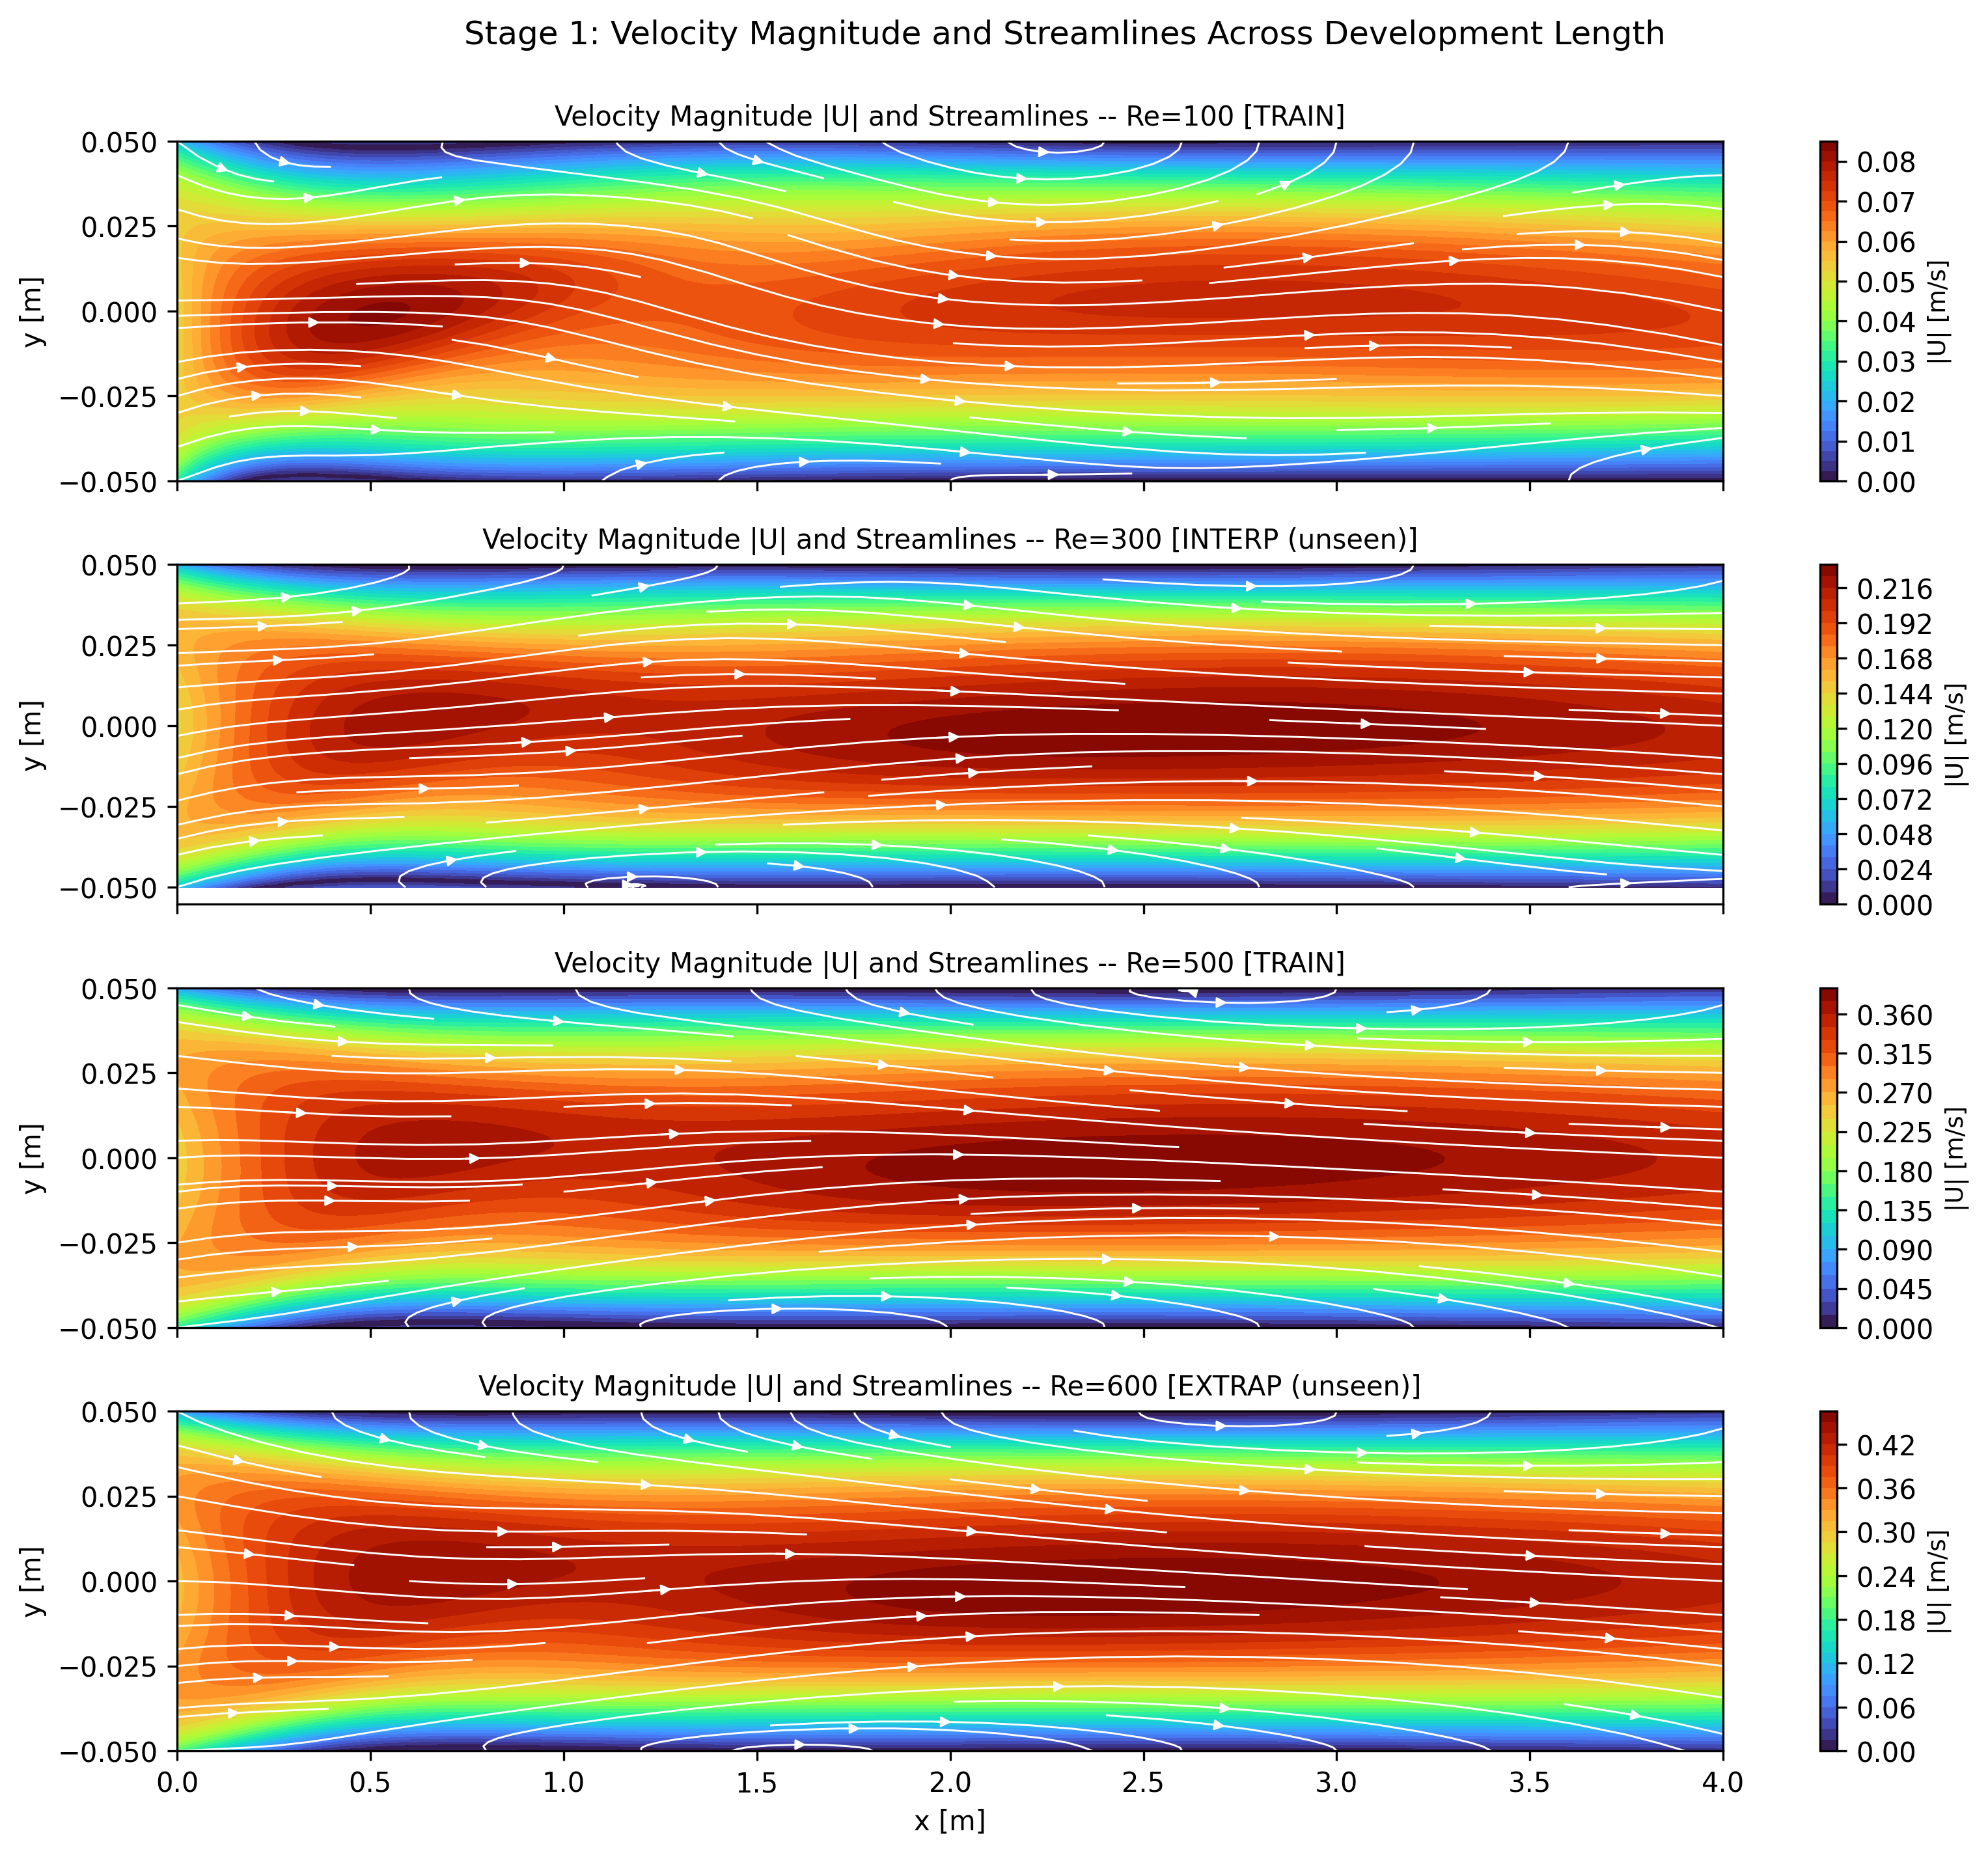
\includegraphics[width=0.85\textwidth]{stage1_flowfield.png}
\caption{Stage 1: Predicted flowfield streamlines and velocity contours across the 2D channel entrance length.}
\label{fig:app_stage1_flowfield}
\end{figure}

\begin{figure}[H]
\centering
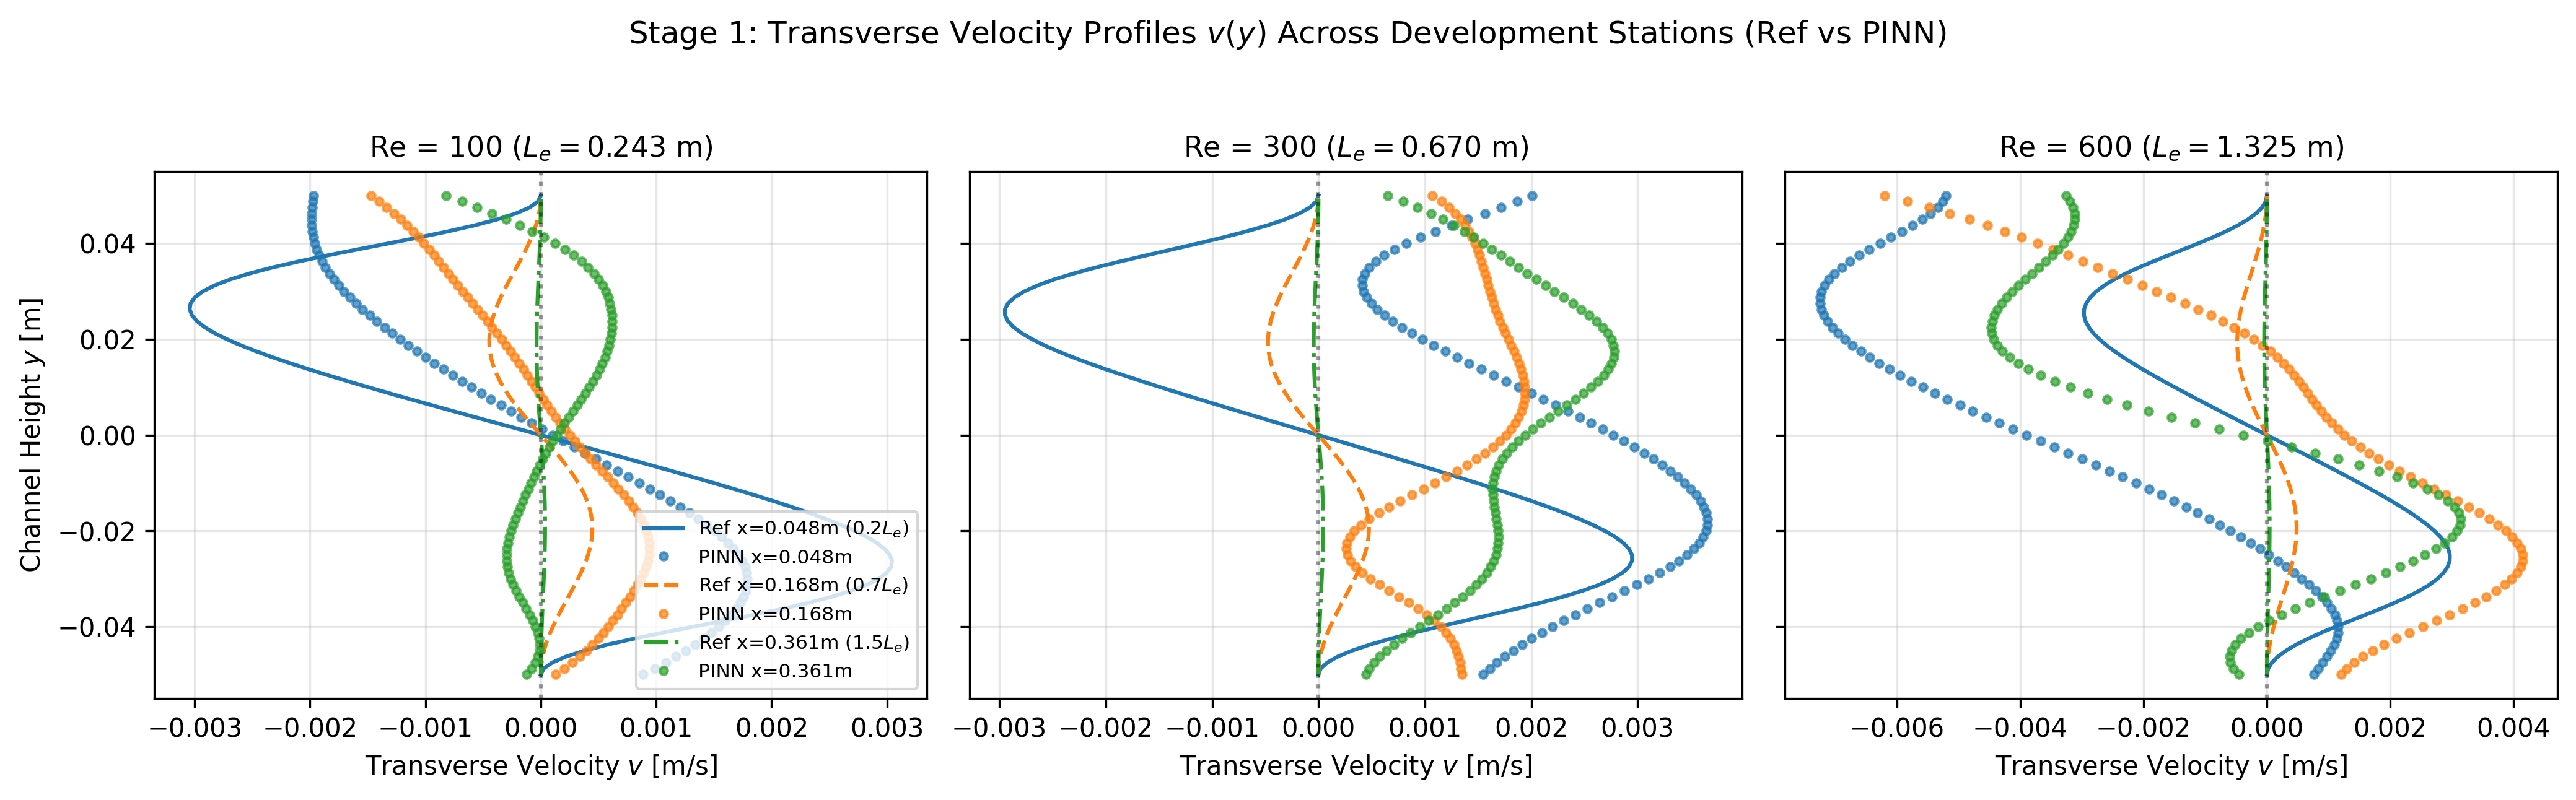
\includegraphics[width=0.85\textwidth]{stage1_v_profiles.png}
\caption{Stage 1: Transverse velocity profiles $v(y)$ compared against reference solver at profile stations $x = 0.243$, $0.670$, and $1.325\,\text{m}$.}
\label{fig:app_stage1_v_profiles}
\end{figure}

\begin{figure}[H]
\centering
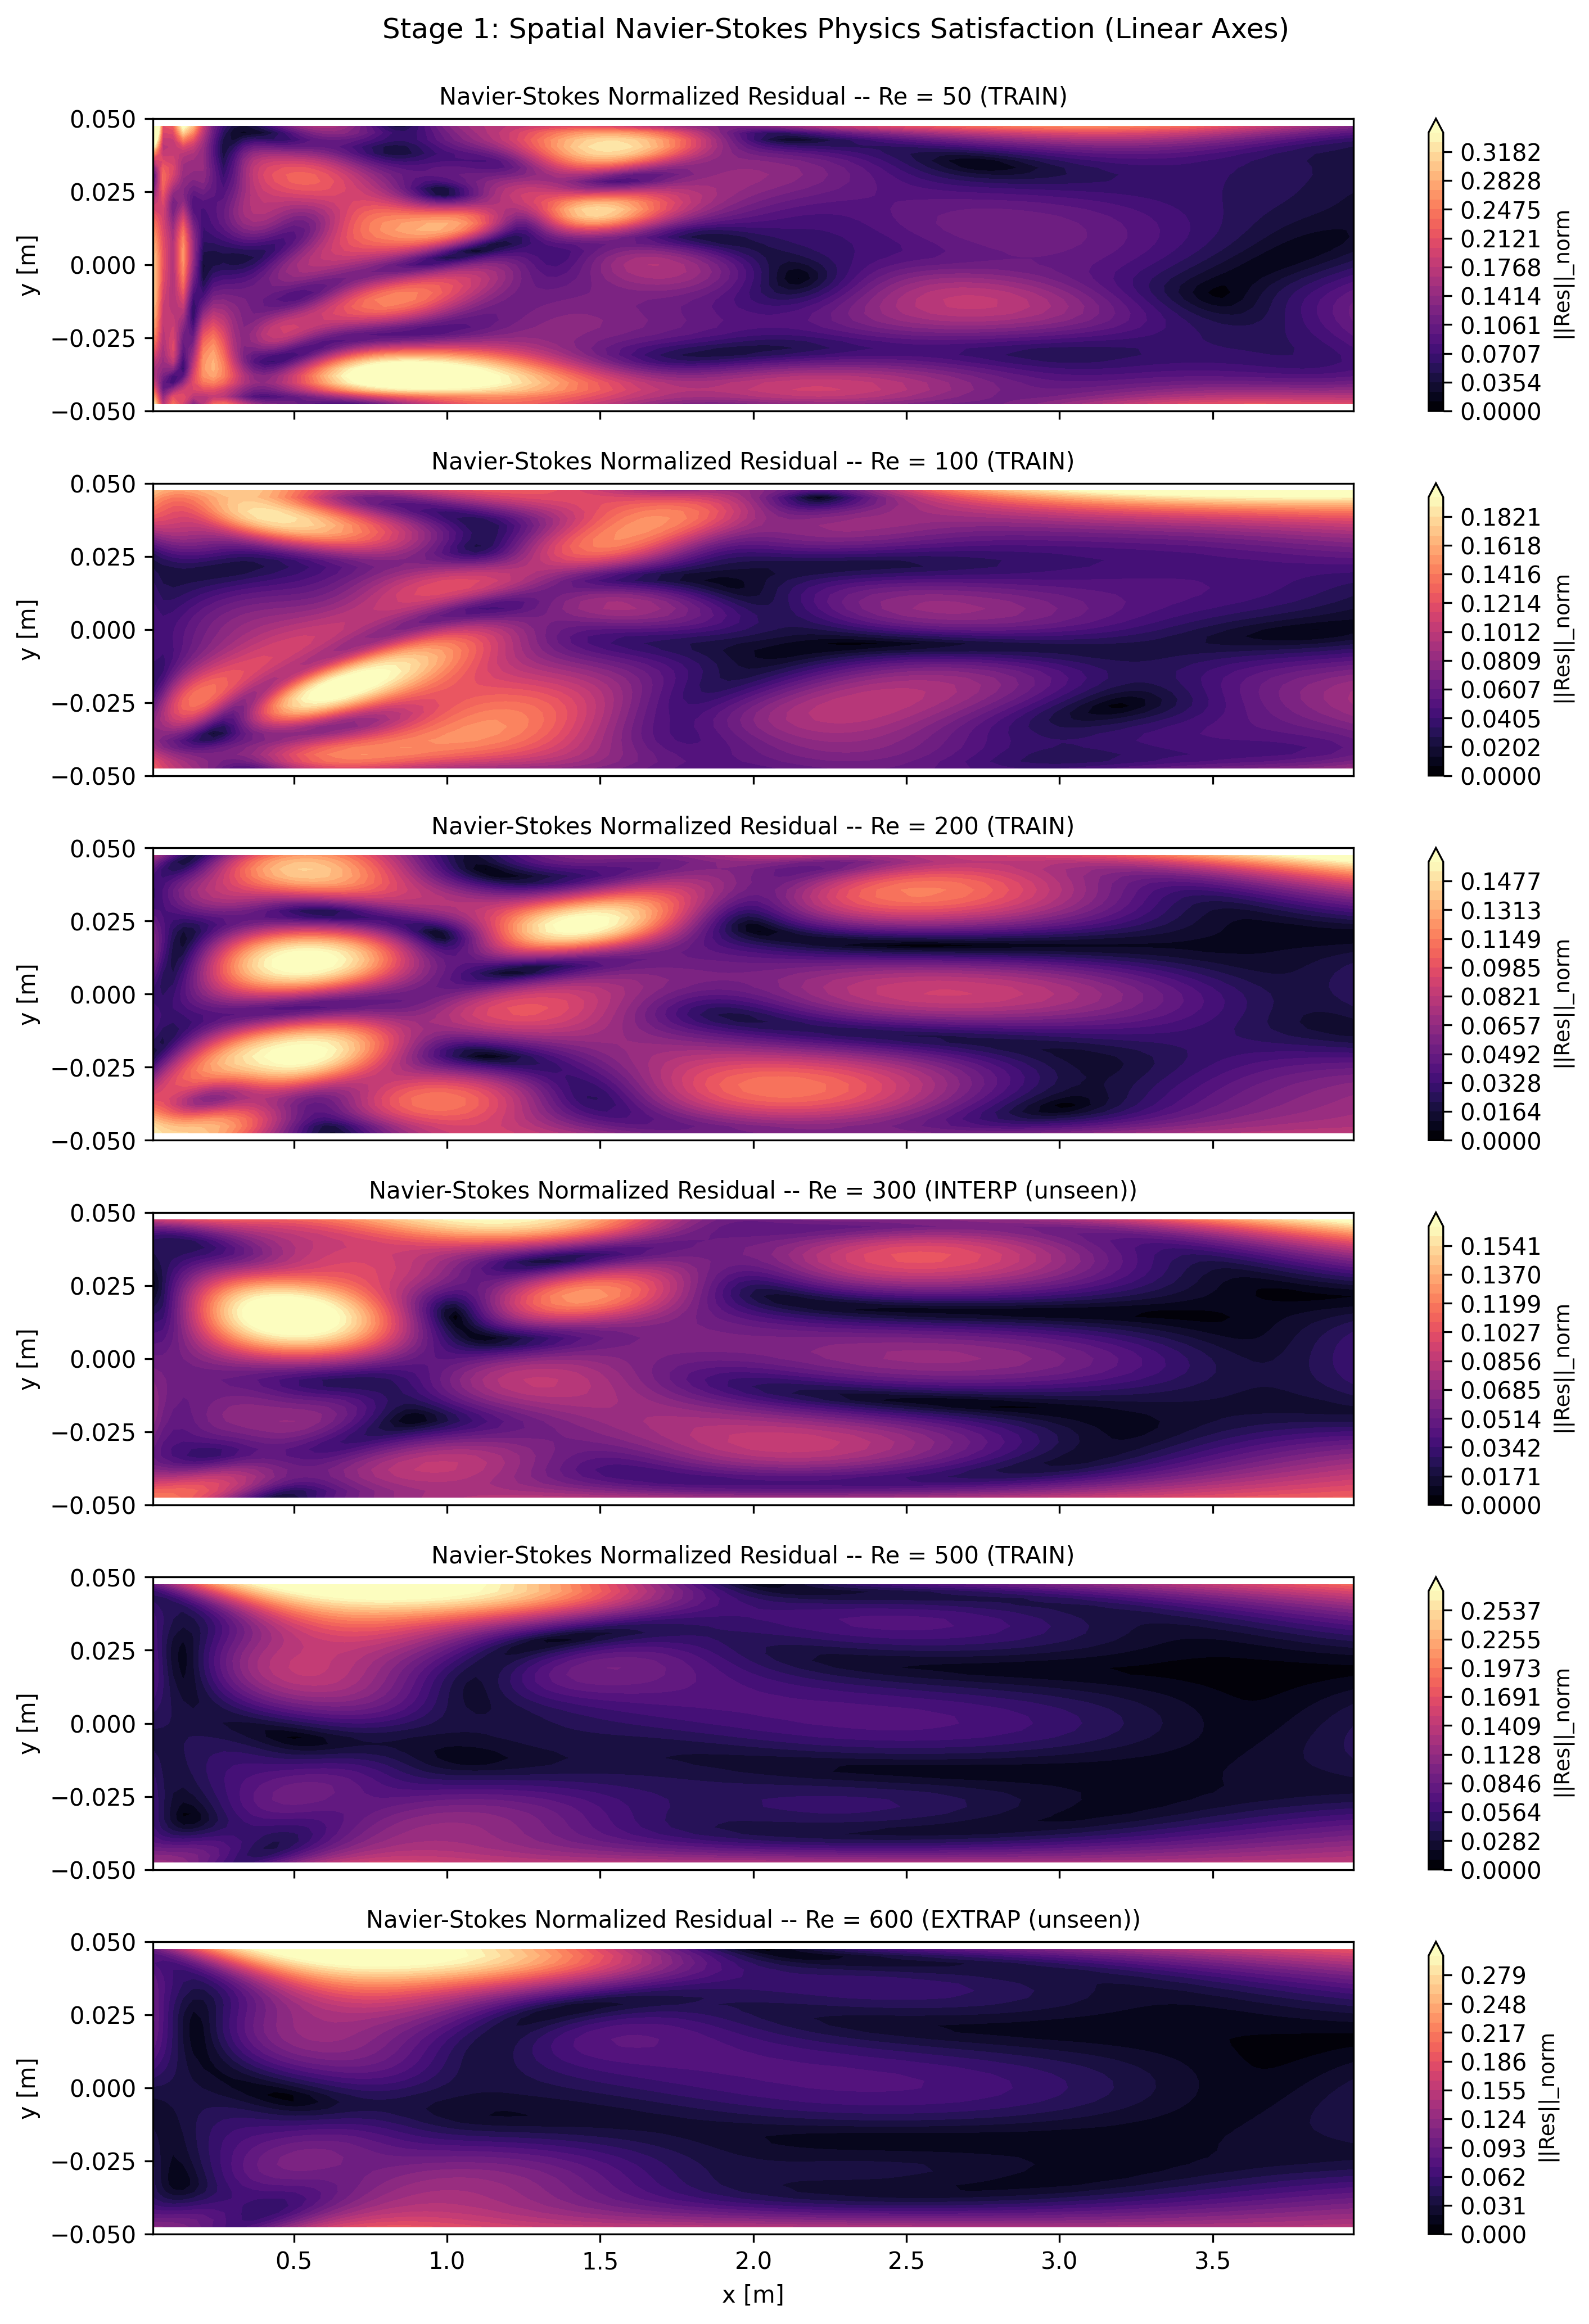
\includegraphics[width=0.85\textwidth]{stage1_residuals.png}
\caption{Stage 1: Spatial distribution of continuity and momentum PDE residuals.}
\label{fig:app_stage1_residuals}
\end{figure}

\clearpage
\subsection{Stage 2: Laminar Pipe Streamlines and Radial Profiles}
\begin{figure}[H]
\centering
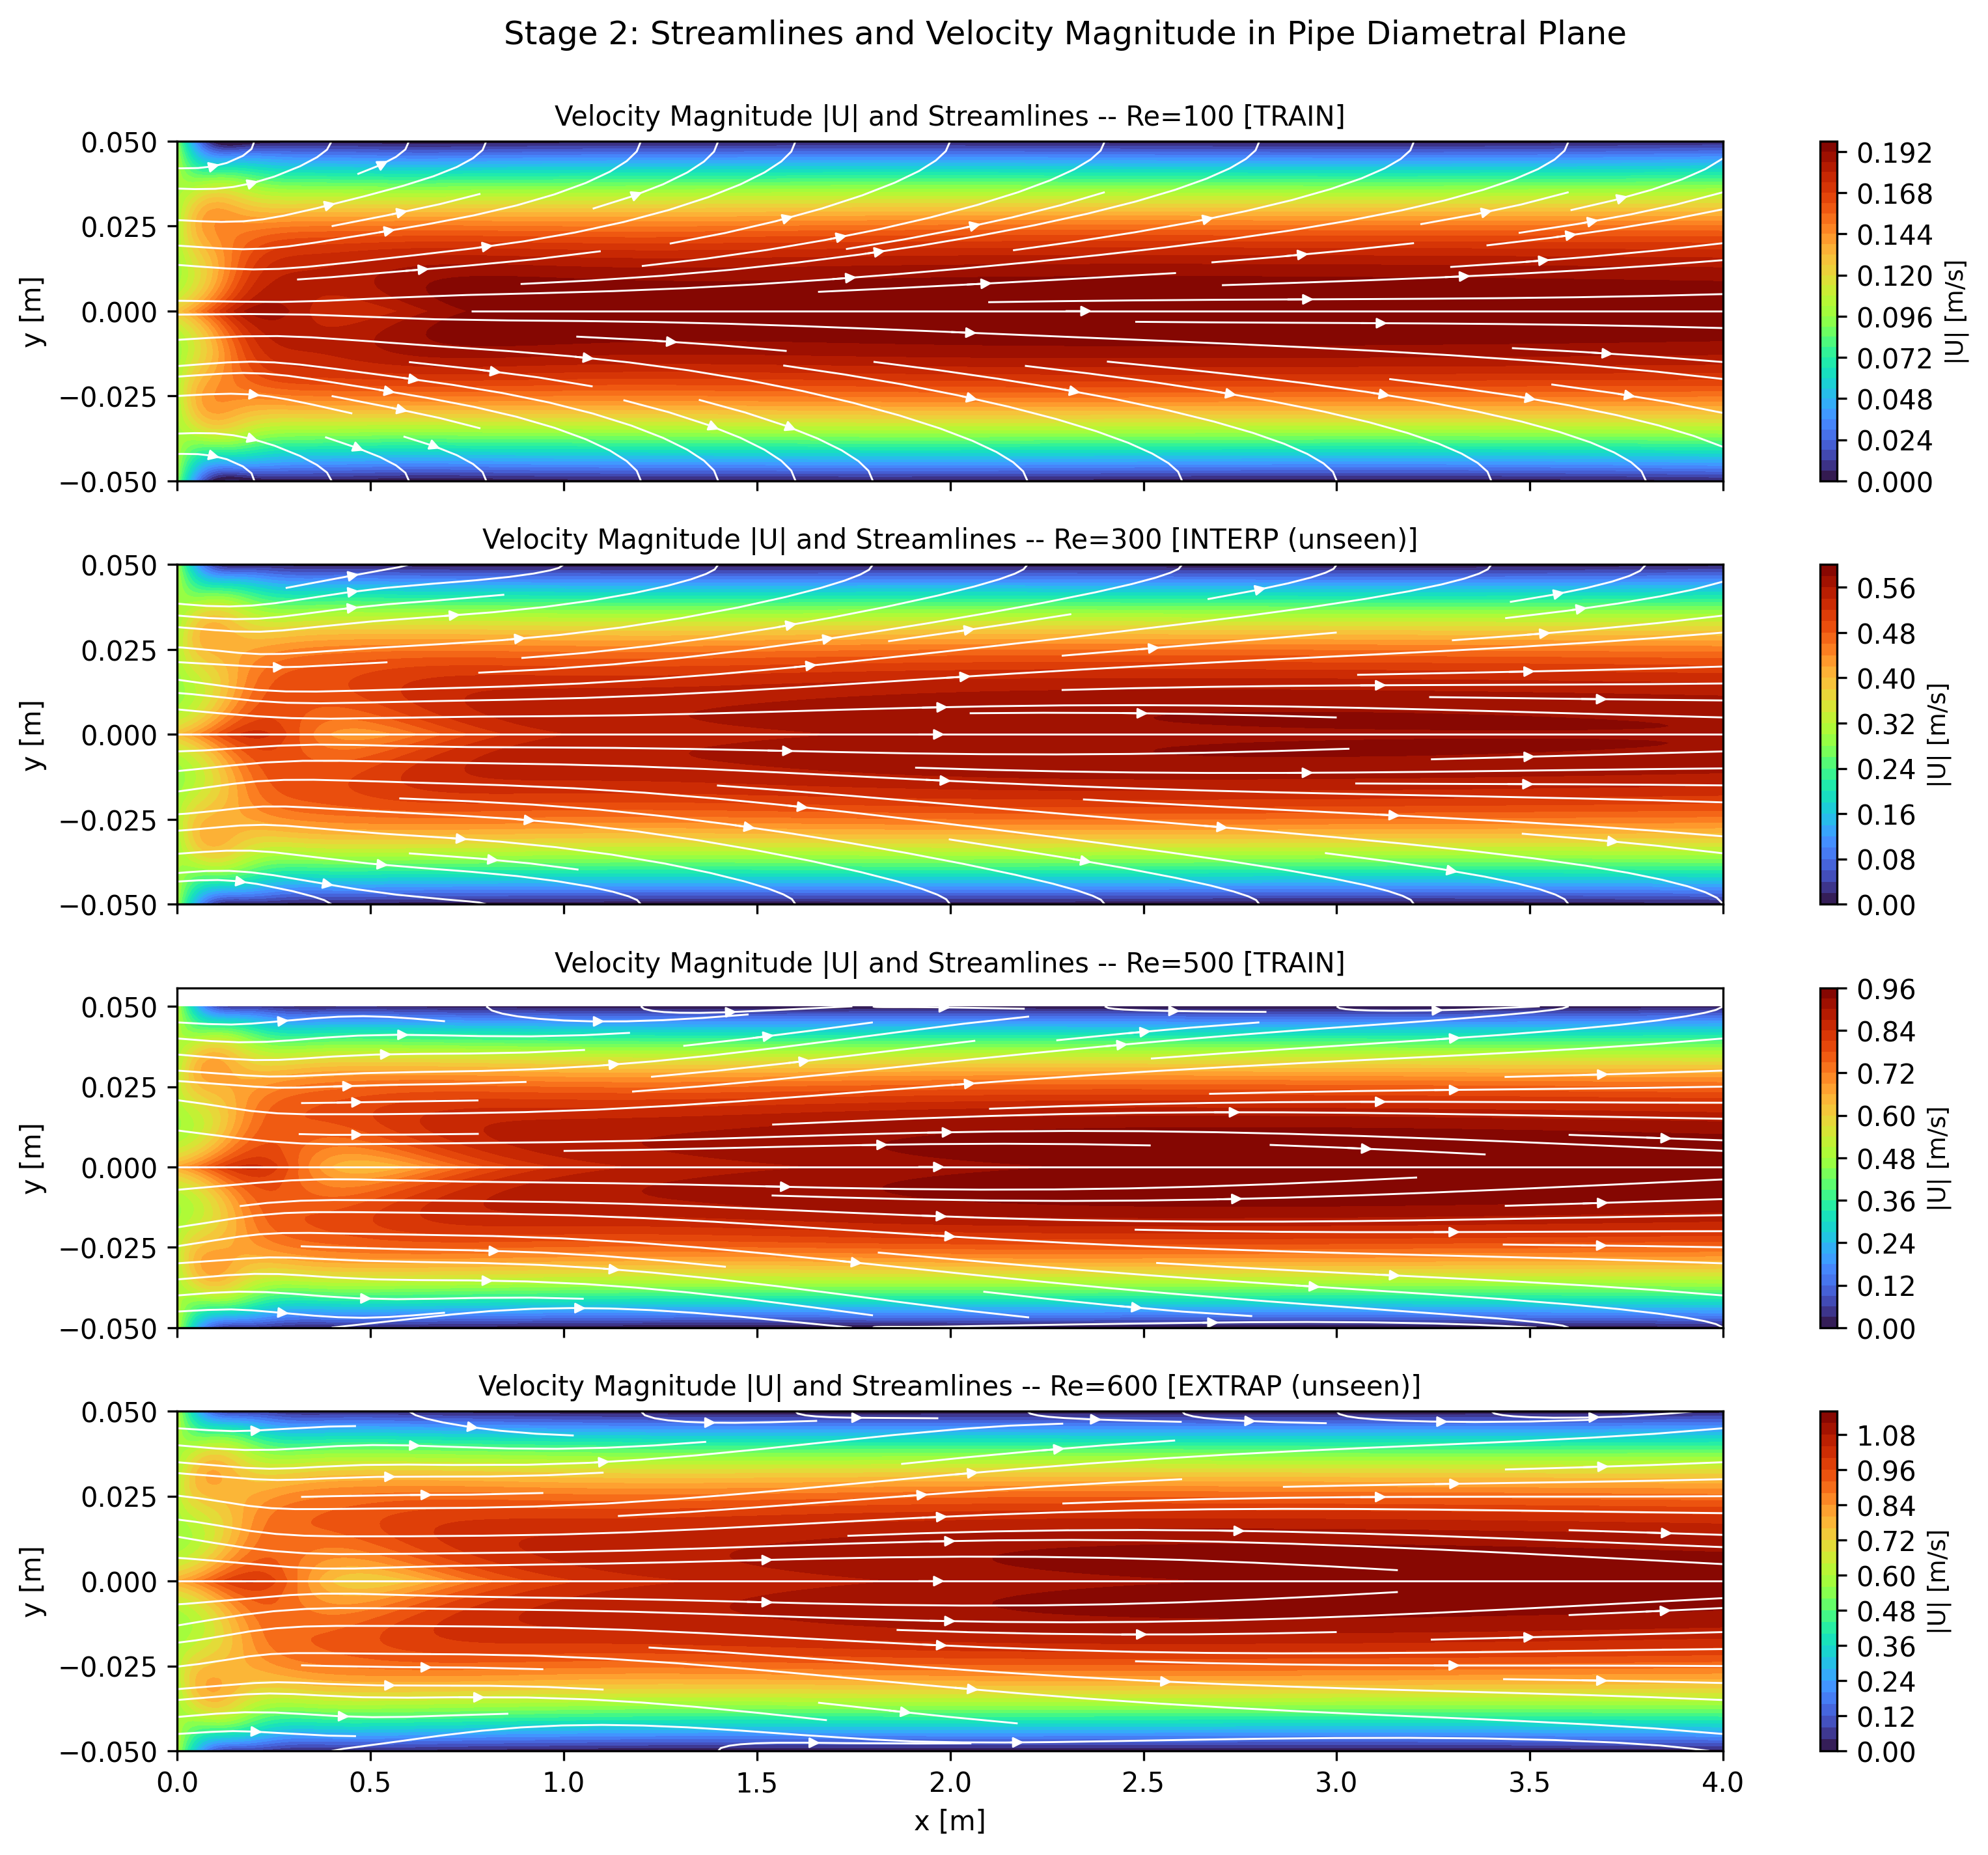
\includegraphics[width=0.85\textwidth]{stage2_flowfield.png}
\caption{Stage 2: Diametral plane velocity magnitude and streamlines in the circular pipe entrance.}
\label{fig:app_stage2_flowfield}
\end{figure}

\begin{figure}[H]
\centering
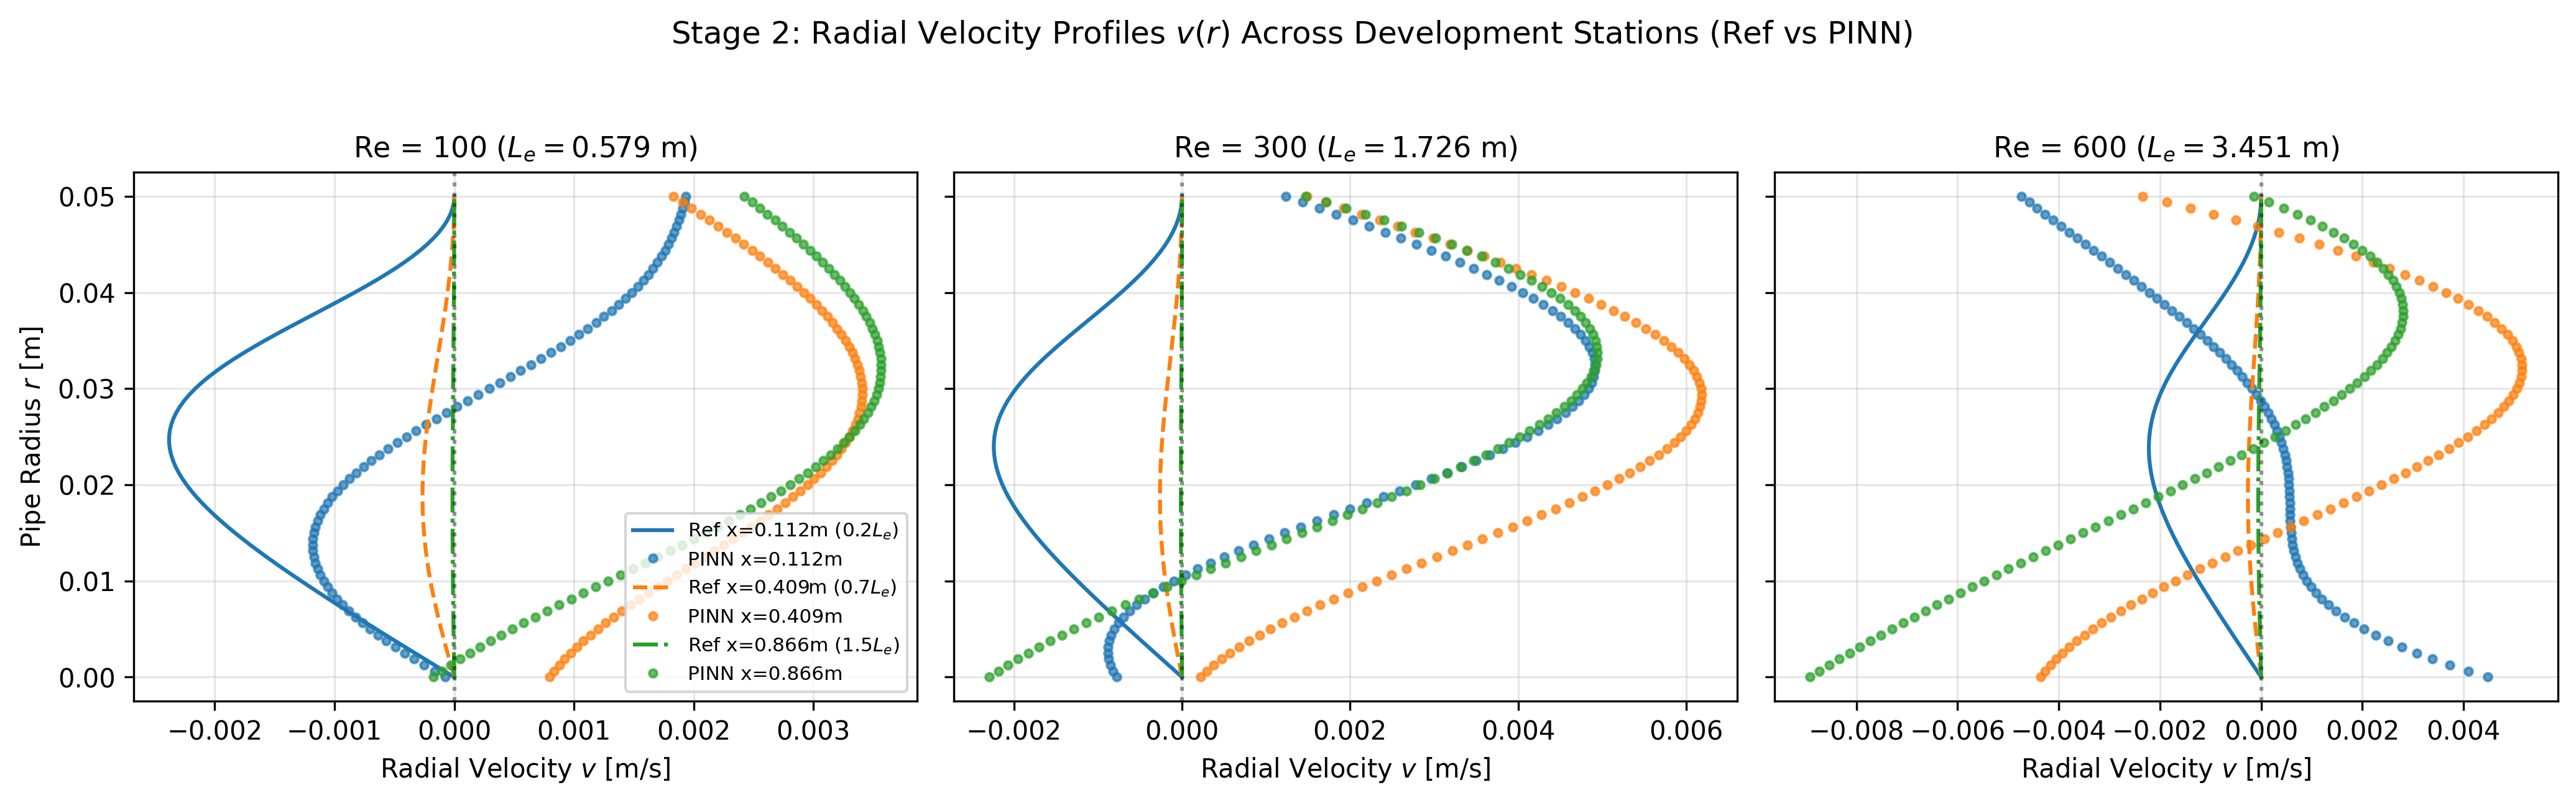
\includegraphics[width=0.85\textwidth]{stage2_v_profiles.png}
\caption{Stage 2: Radial velocity profiles $v(r)$ compared against Hornbeck reference marching solver.}
\label{fig:app_stage2_v_profiles}
\end{figure}

\begin{figure}[H]
\centering
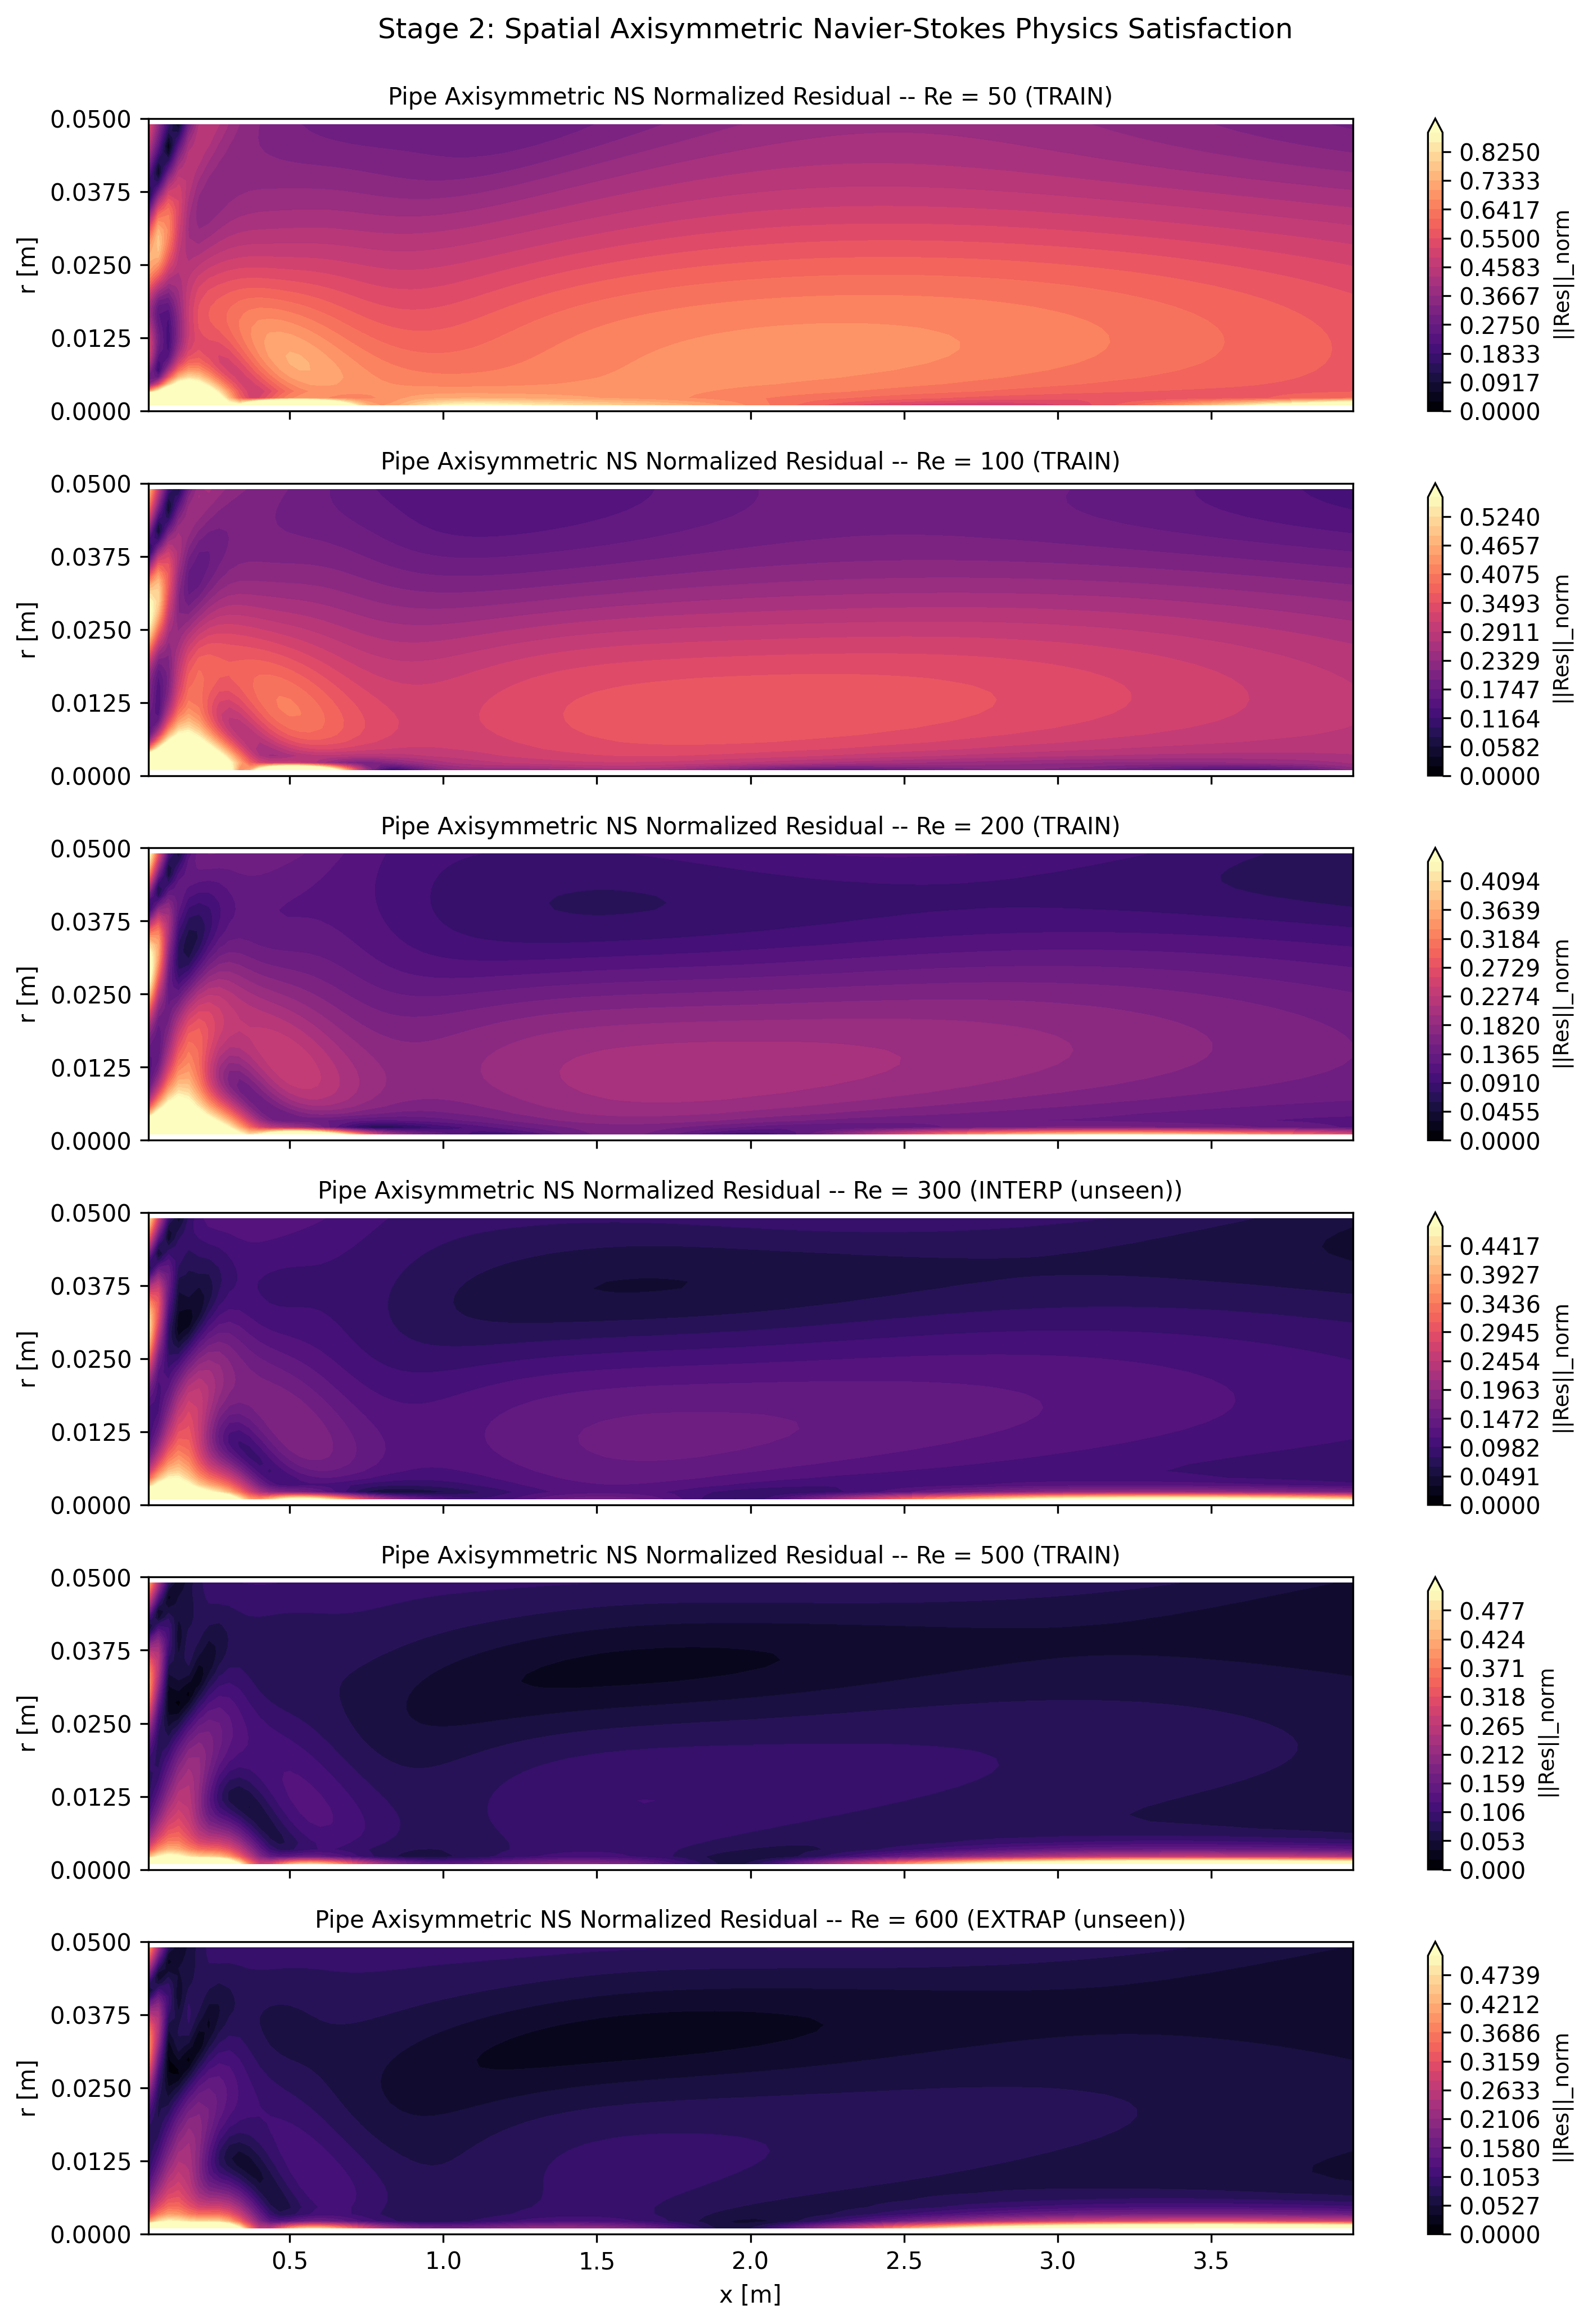
\includegraphics[width=0.85\textwidth]{stage2_residuals.png}
\caption{Stage 2: Axisymmetric continuity and momentum equation residuals.}
\label{fig:app_stage2_residuals}
\end{figure}

\clearpage
\subsection{Stage 3: 3D Duct Cross-Planes and Analytical Fourier Solution}
\begin{figure}[H]
\centering
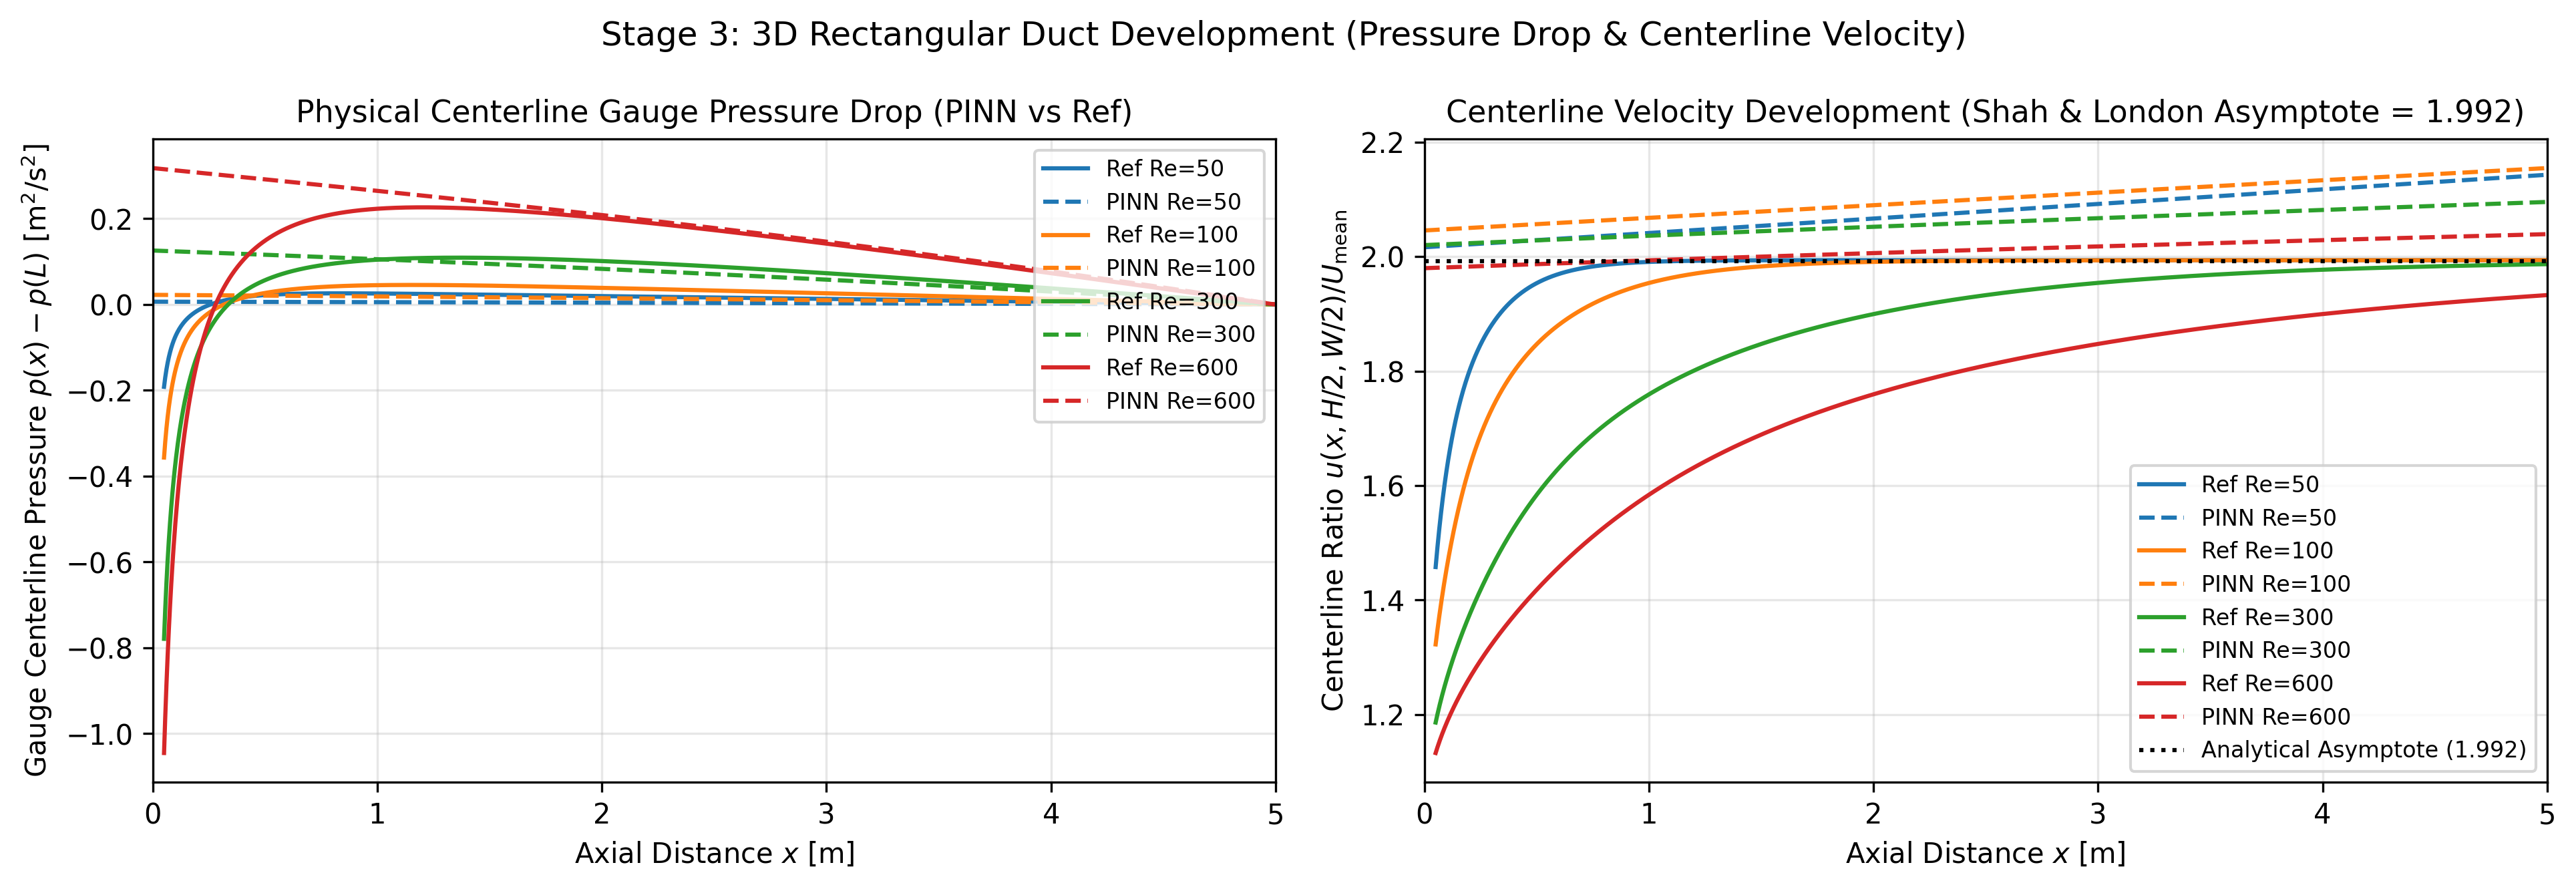
\includegraphics[width=0.85\textwidth]{duct_centerline_p_comparison.png}
\caption{Stage 3: Centerline pressure distribution comparing PINN against reference marching solver across Re, showing the inlet reference transient and downstream gradient differences.}
\label{fig:app_stage3_p_centerline}
\end{figure}

\begin{figure}[H]
\centering
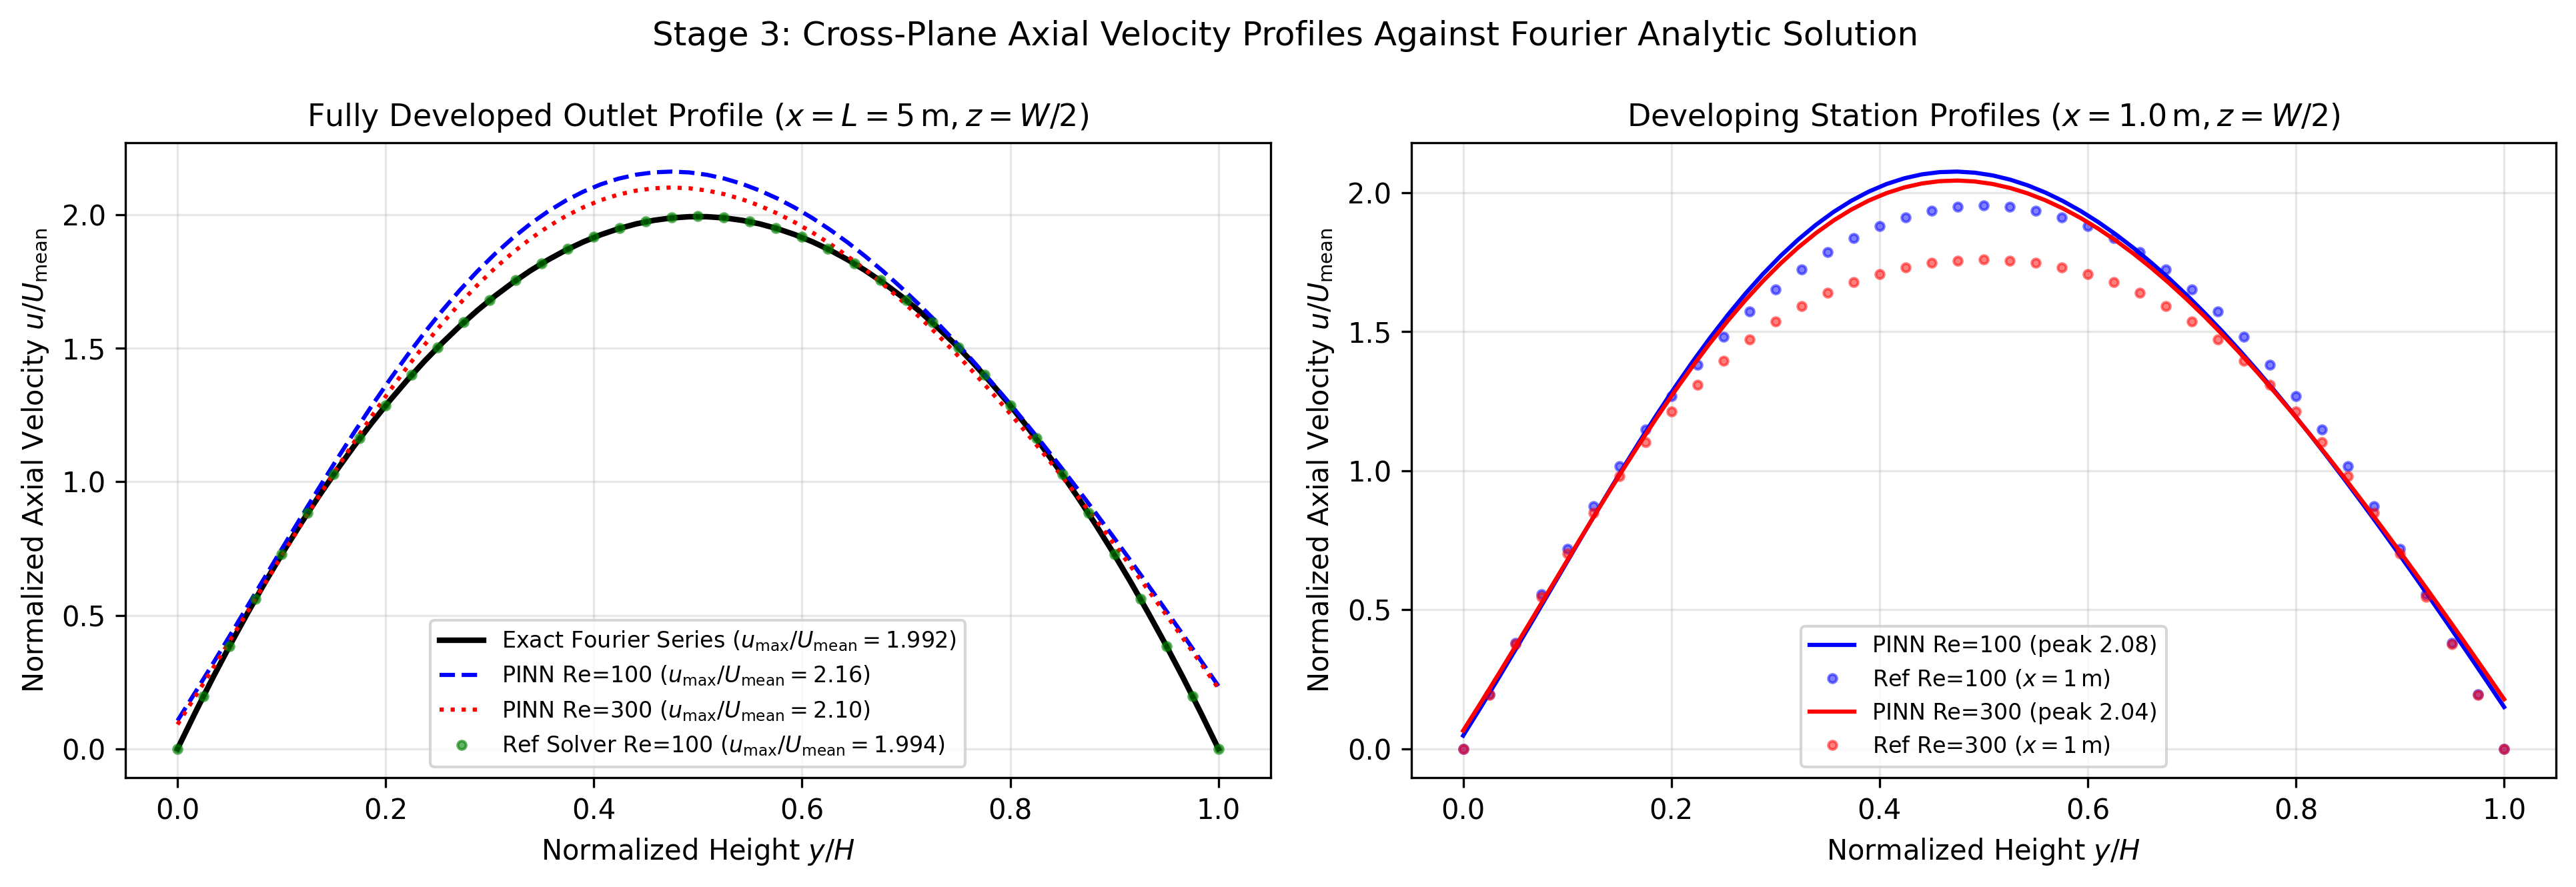
\includegraphics[width=0.85\textwidth]{duct_fourier_analytical_comparison.png}
\caption{Stage 3: Cross-plane axial velocity profiles compared against the Shah and London analytical Fourier series solution ($u_{\max}/U_{\mathrm{mean}} = 1.992$). Left: exit plane ($x=5.0\,\mathrm{m}$); right: developing station ($x=1.0\,\mathrm{m}$).}
\label{fig:app_stage3_fourier}
\end{figure}

\begin{figure}[H]
\centering
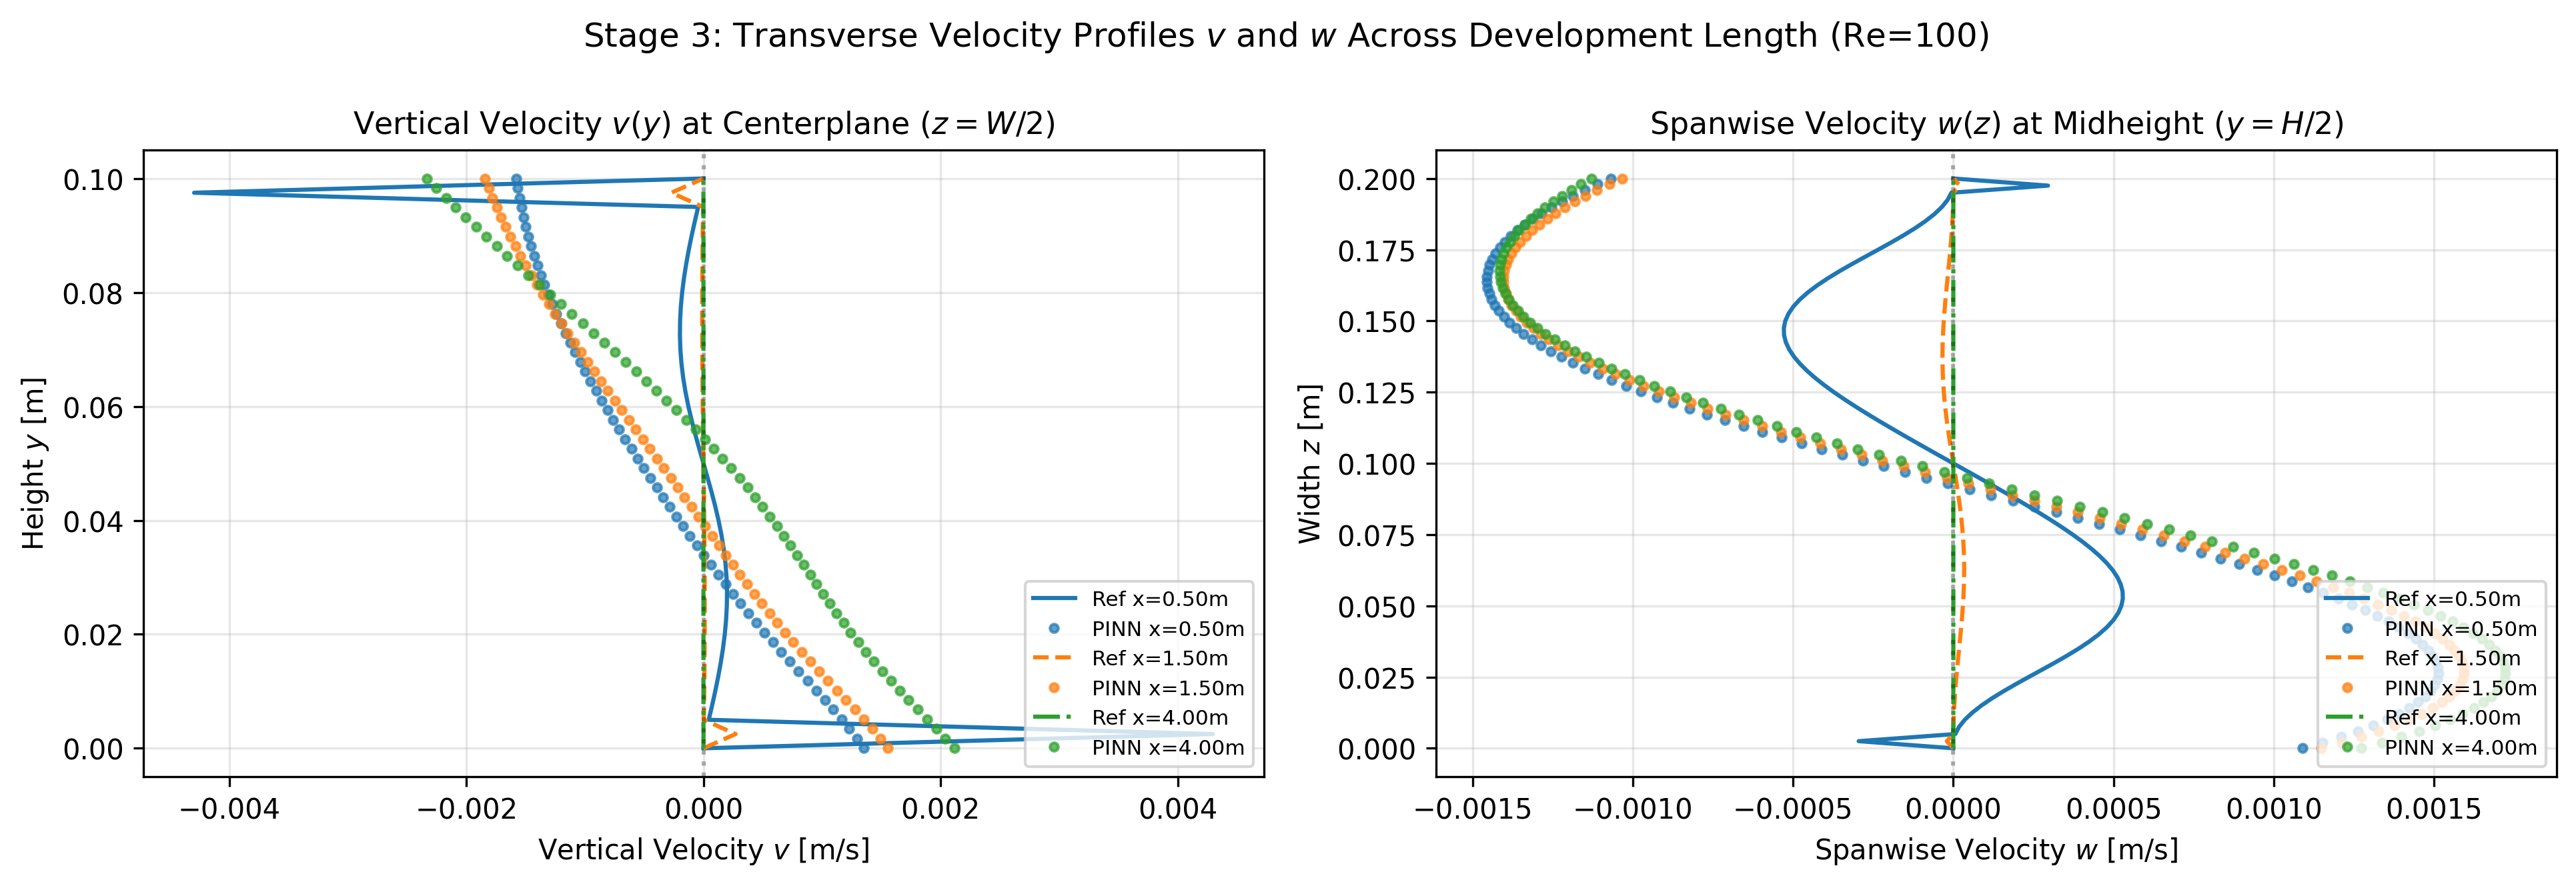
\includegraphics[width=0.85\textwidth]{stage3_vw_profiles.png}
\caption{Stage 3: Transverse cross-stream velocity components $v(y)$ and $w(z)$ along duct development length.}
\label{fig:app_stage3_vw_profiles}
\end{figure}

\clearpage
\subsection{Stage 4: Turbulent Channel Eddy Viscosity and Residuals}
\begin{figure}[H]
\centering
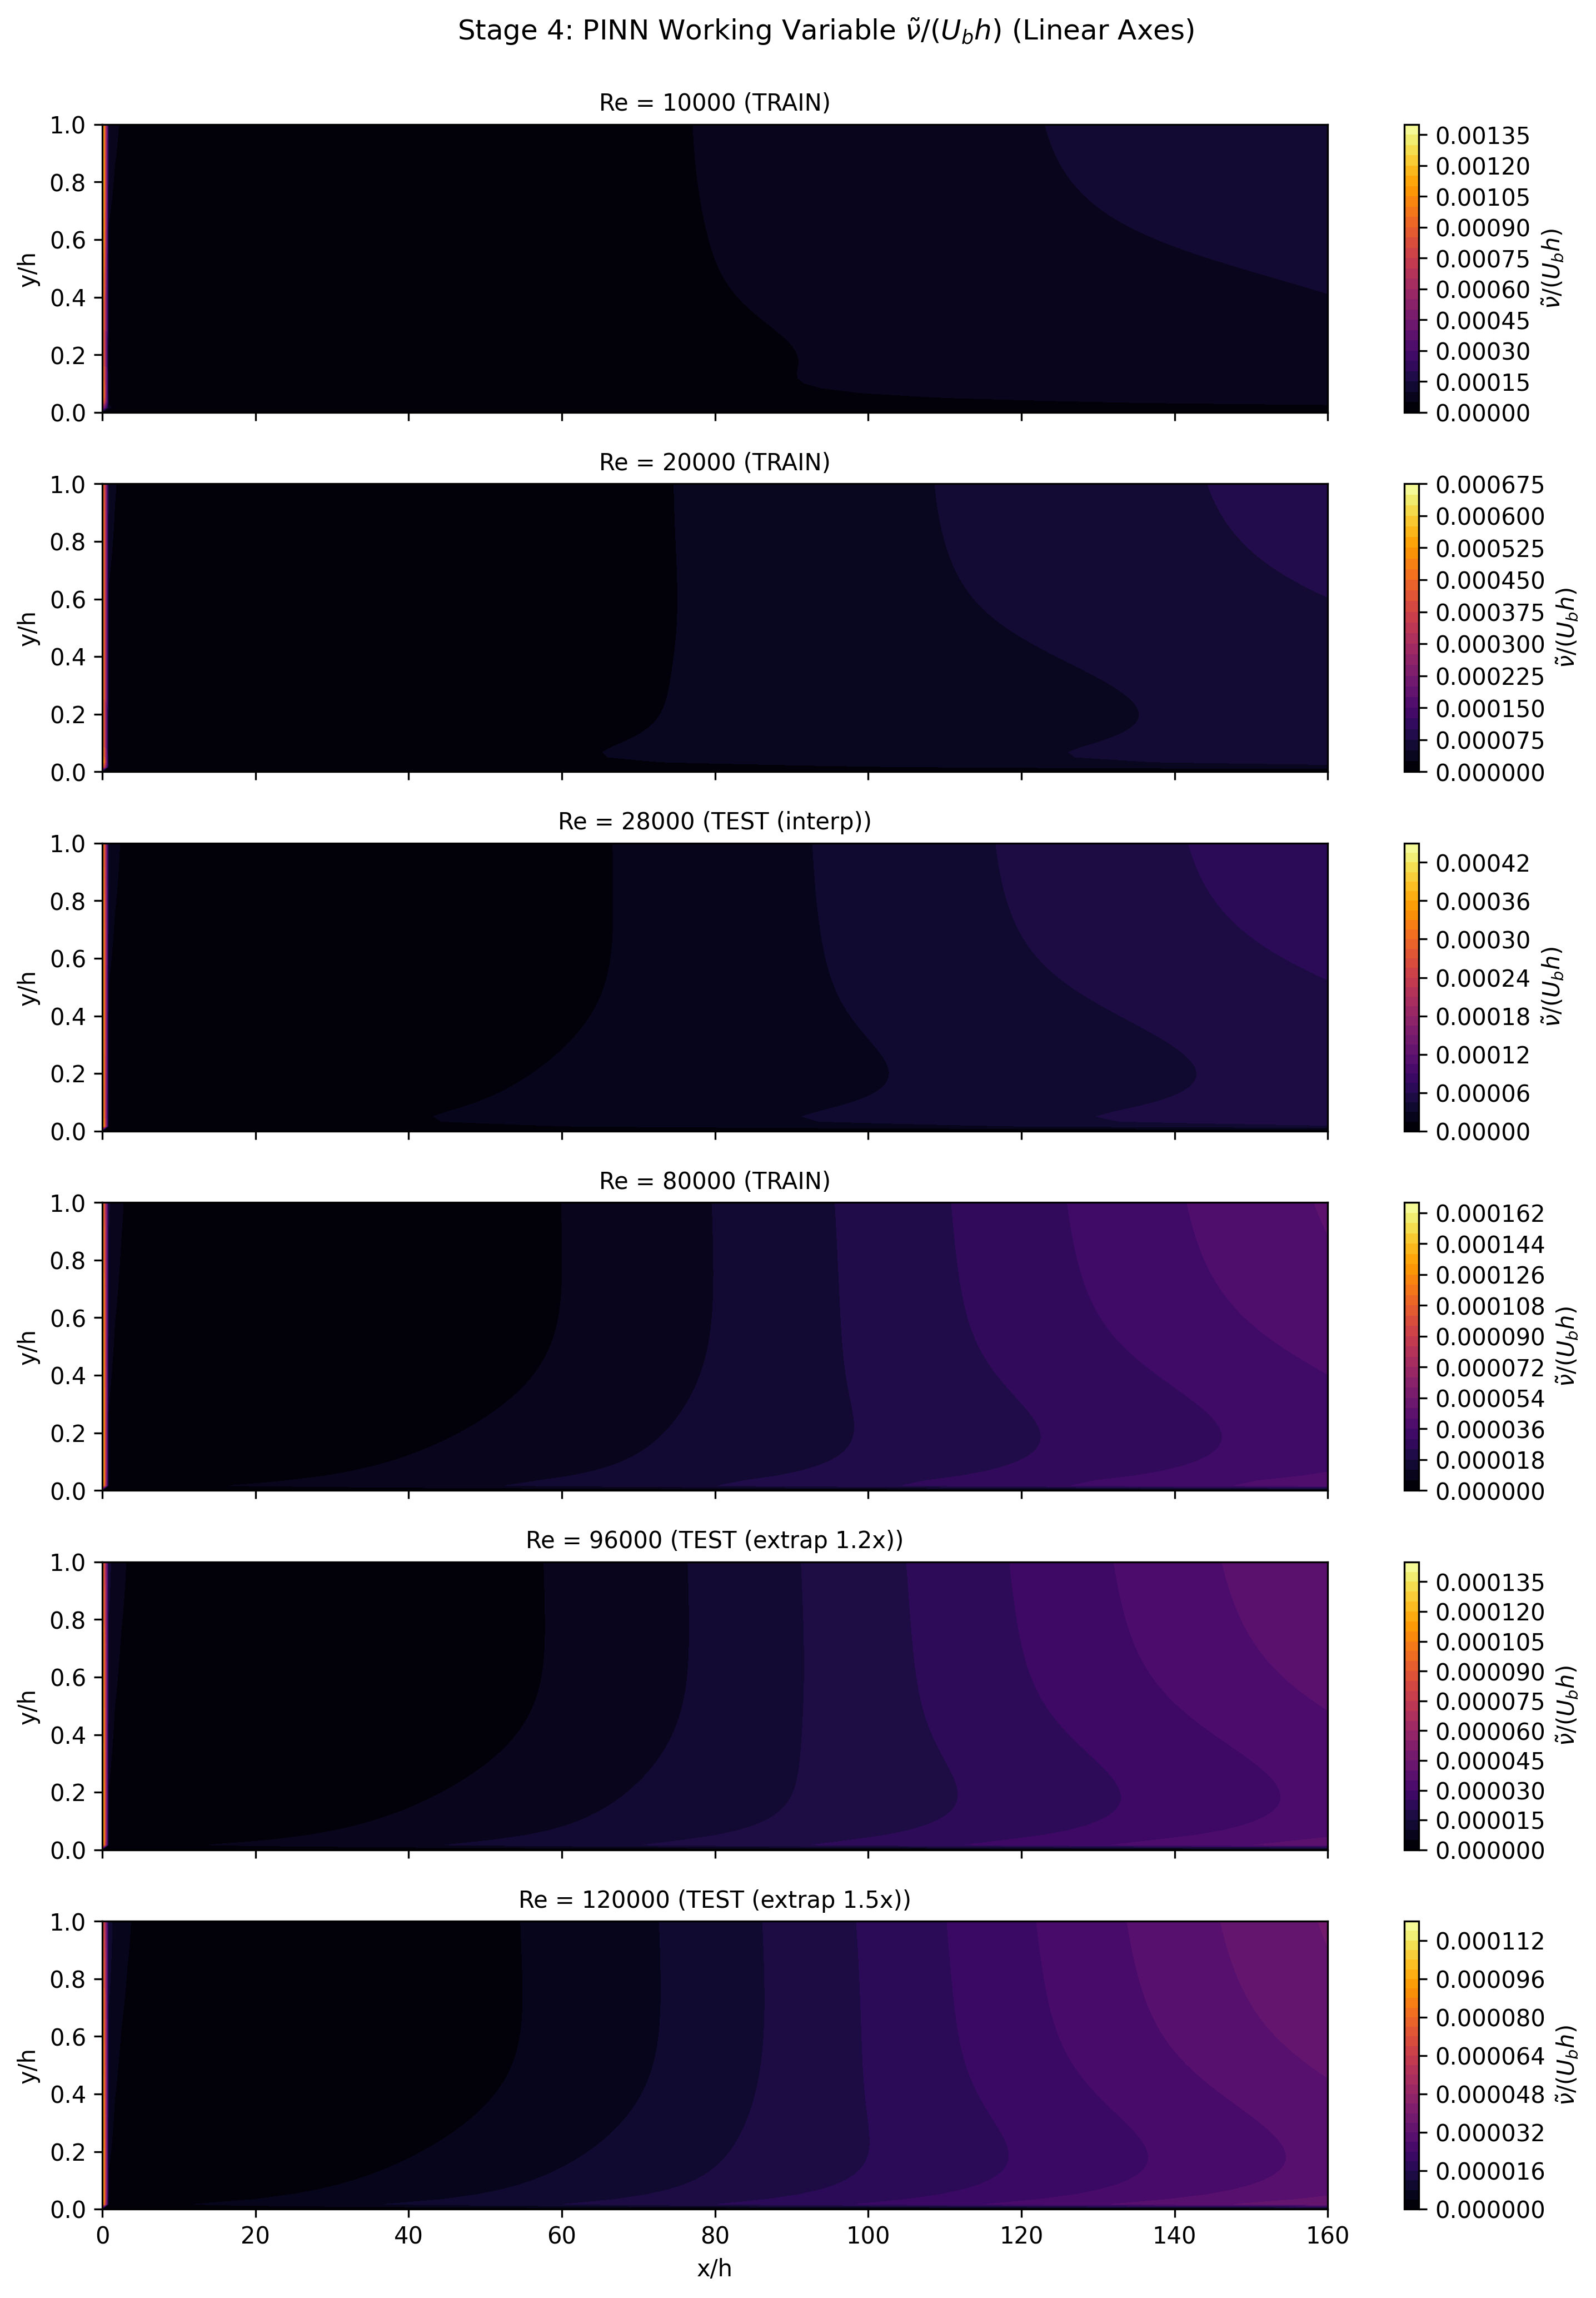
\includegraphics[width=0.85\textwidth]{channel_turb_flowfield_pinn_nut.png}
\caption{Stage 4: PINN predicted turbulent working variable $\tilde{\nu}/(U_b h)$ illustrating eddy viscosity extinction.}
\label{fig:app_stage4_nut}
\end{figure}

\begin{figure}[H]
\centering
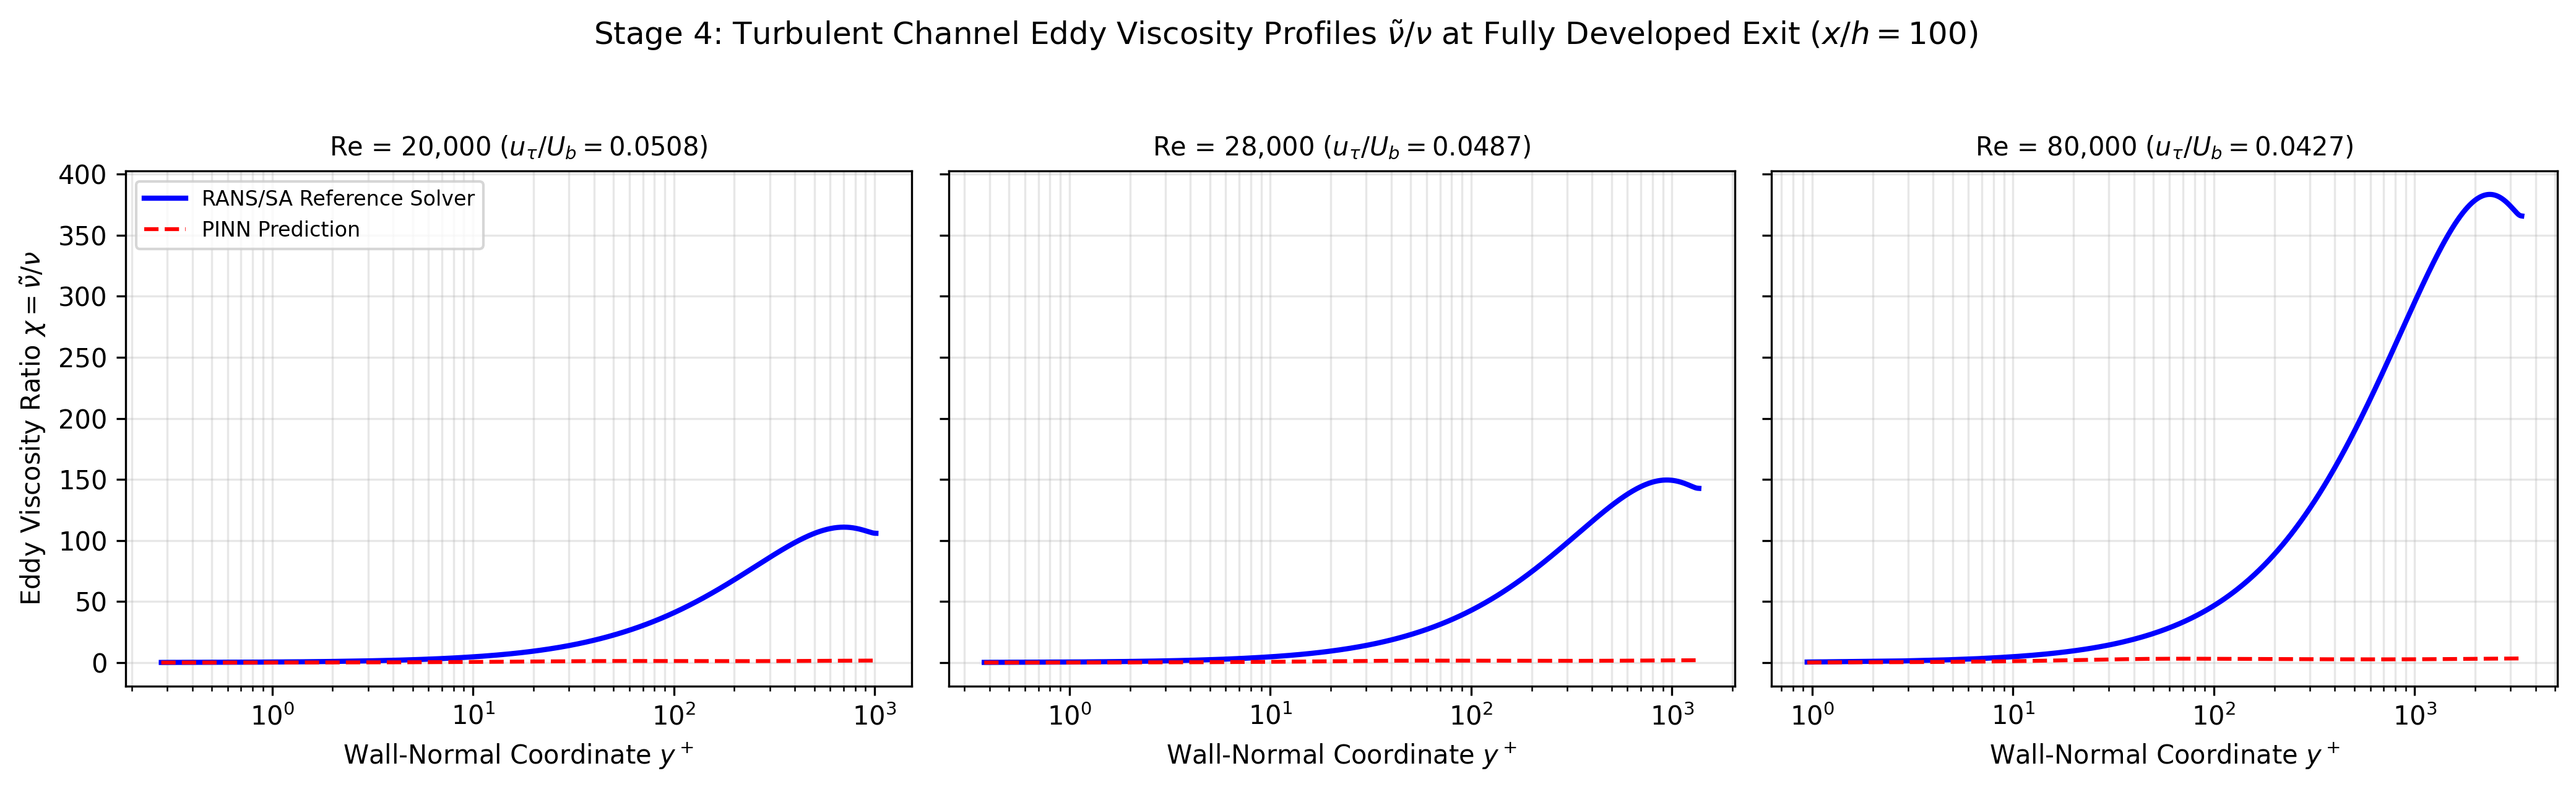
\includegraphics[width=0.85\textwidth]{stage4_nut_profiles_yplus.png}
\caption{Stage 4: Wall-normal eddy viscosity profiles $\tilde{\nu}^+(y^+)$ comparing PINN against reference solver.}
\label{fig:app_stage4_nut_yplus}
\end{figure}

\begin{figure}[H]
\centering
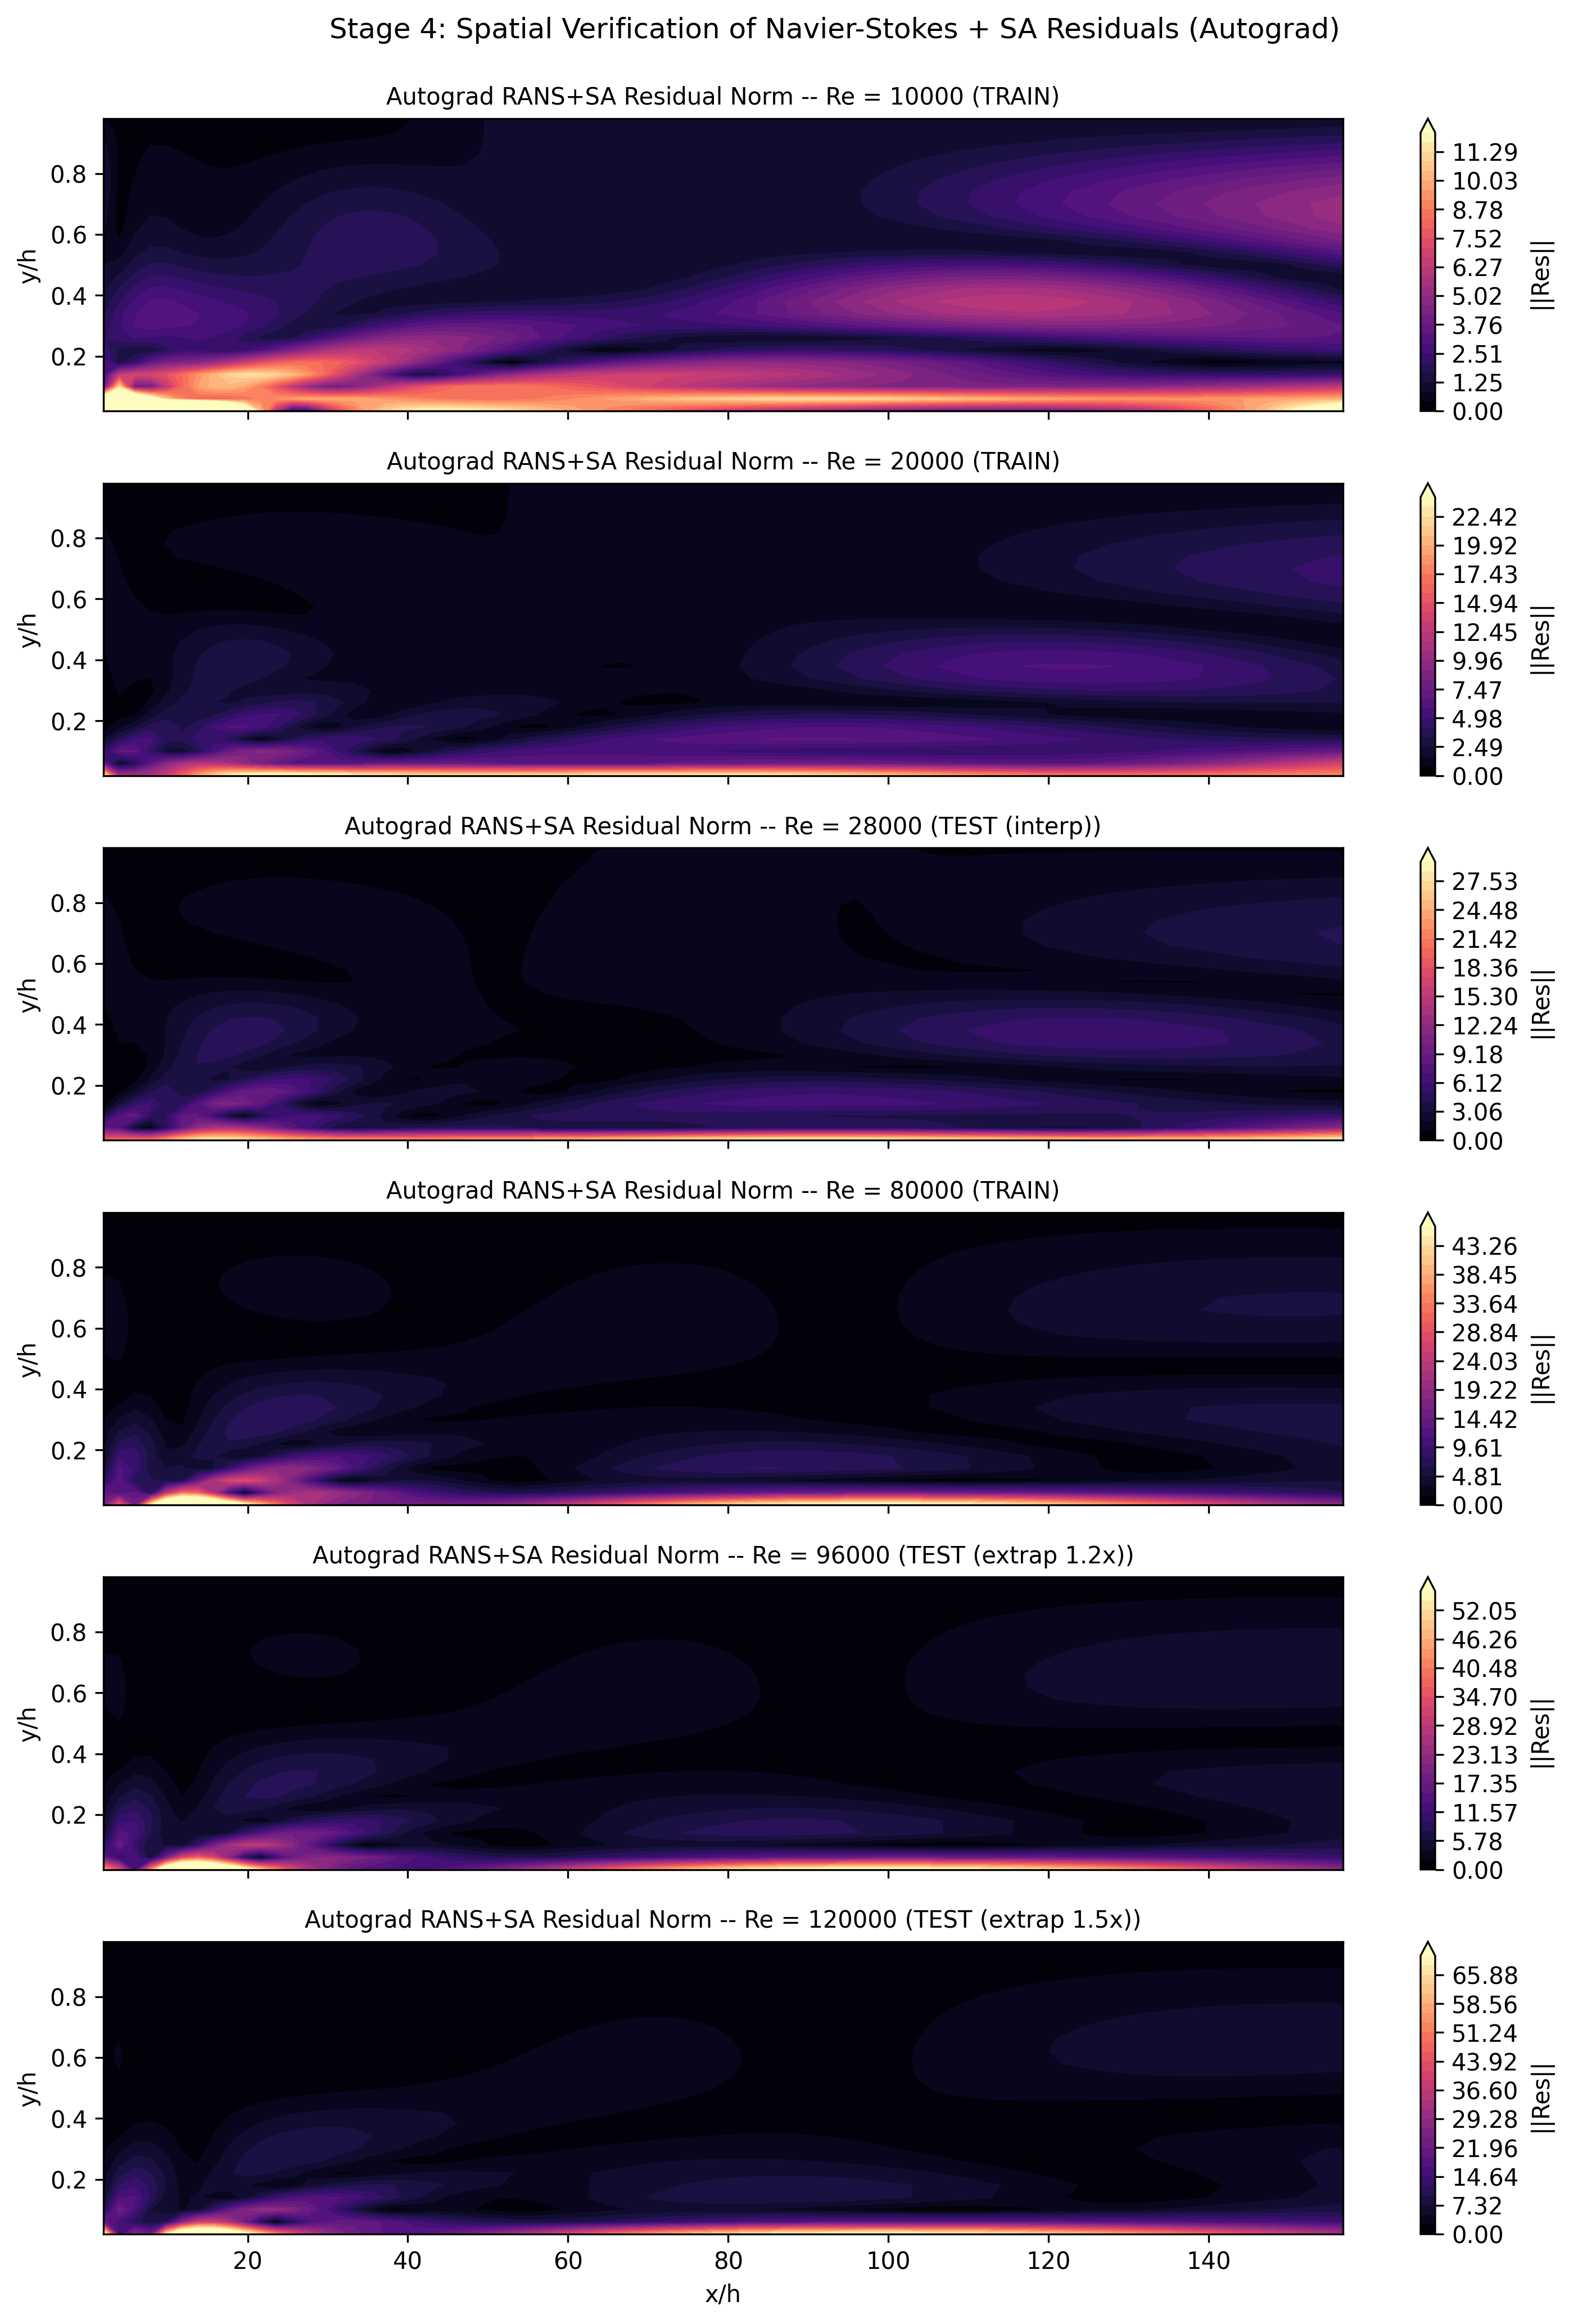
\includegraphics[width=0.85\textwidth]{stage4_residuals.png}
\caption{Stage 4: Whole-domain RANS momentum and Spalart--Allmaras equation residuals.}
\label{fig:app_stage4_residuals}
\end{figure}

\clearpage
\subsection{Stage 5: Turbulent Pipe Eddy Viscosity and Residuals}
\begin{figure}[H]
\centering
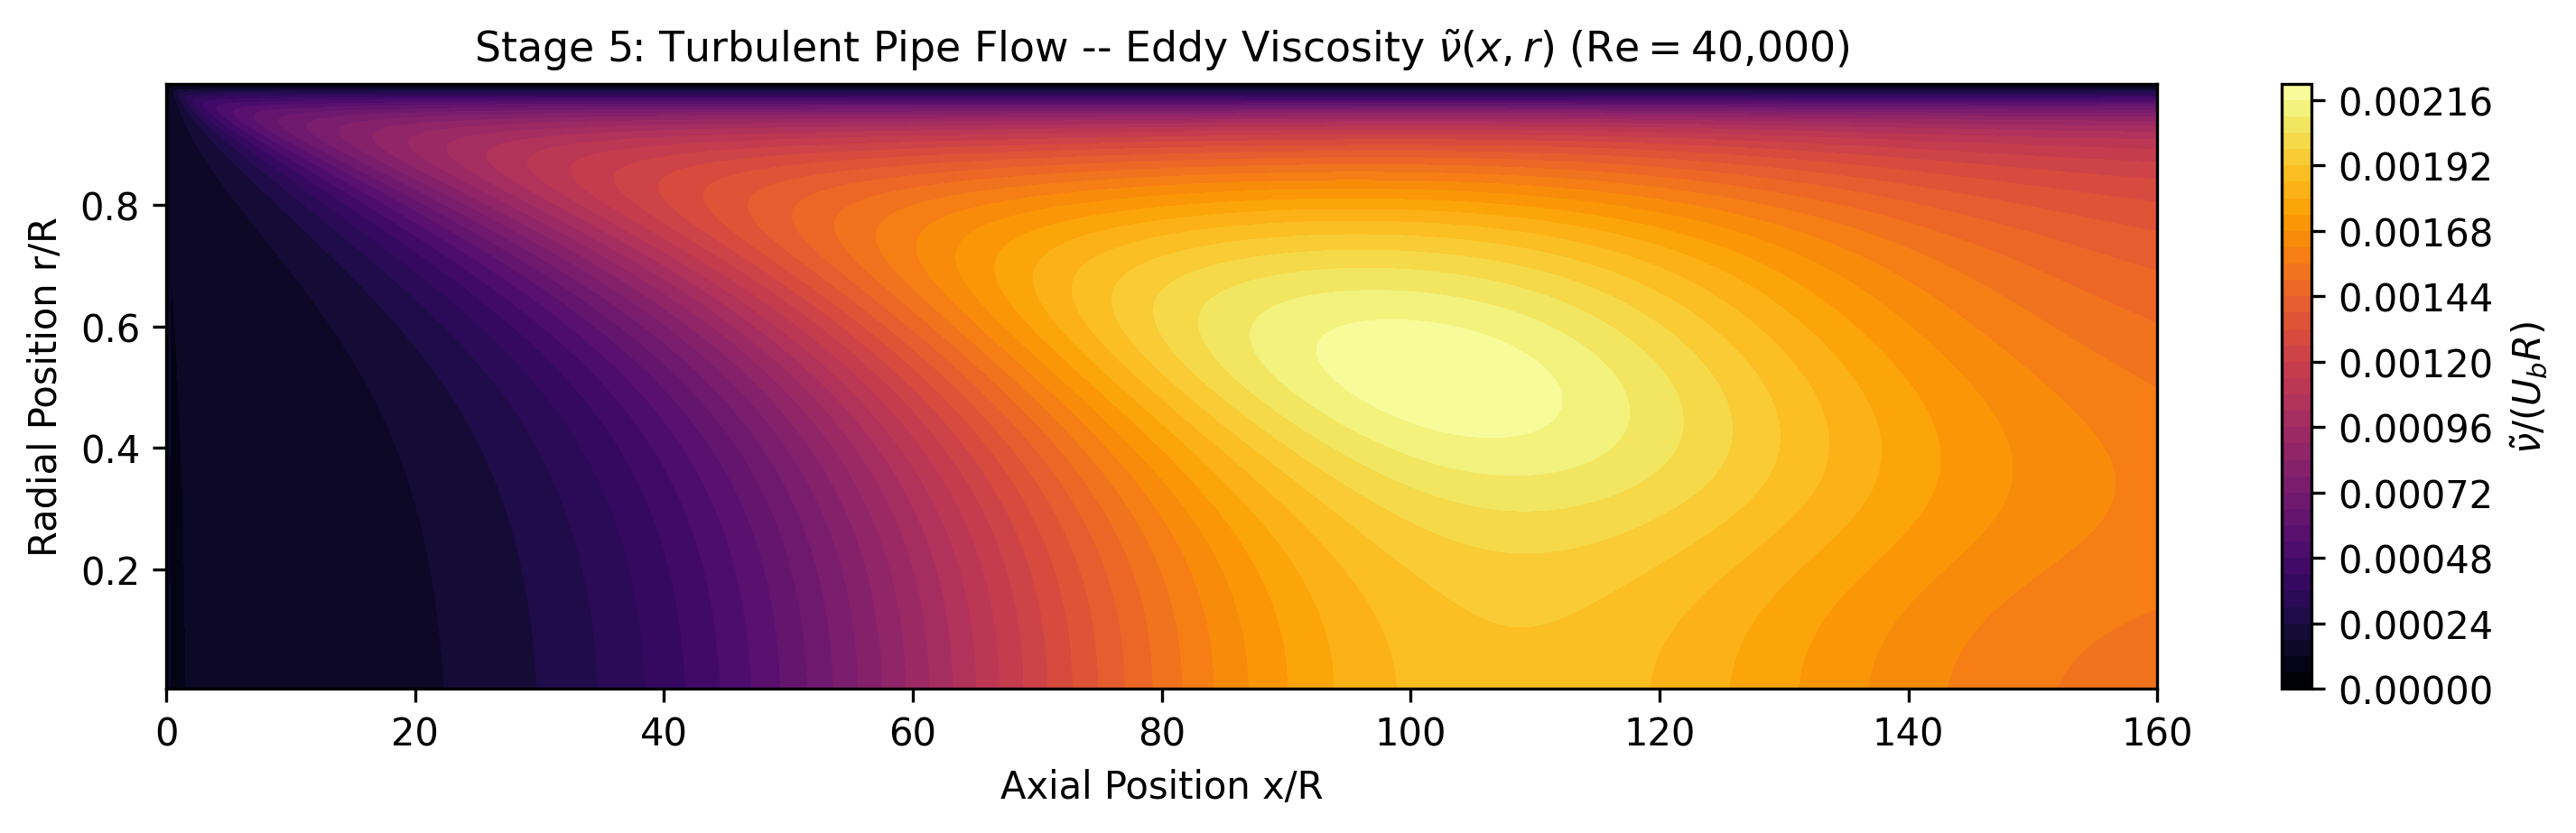
\includegraphics[width=0.85\textwidth]{pipe_turb_flowfield_pinn_nut.png}
\caption{Stage 5: PINN predicted eddy viscosity $\tilde{\nu}/(U_b R)$ showing partial recovery in cylindrical coordinates.}
\label{fig:app_stage5_nut}
\end{figure}

\begin{figure}[H]
\centering
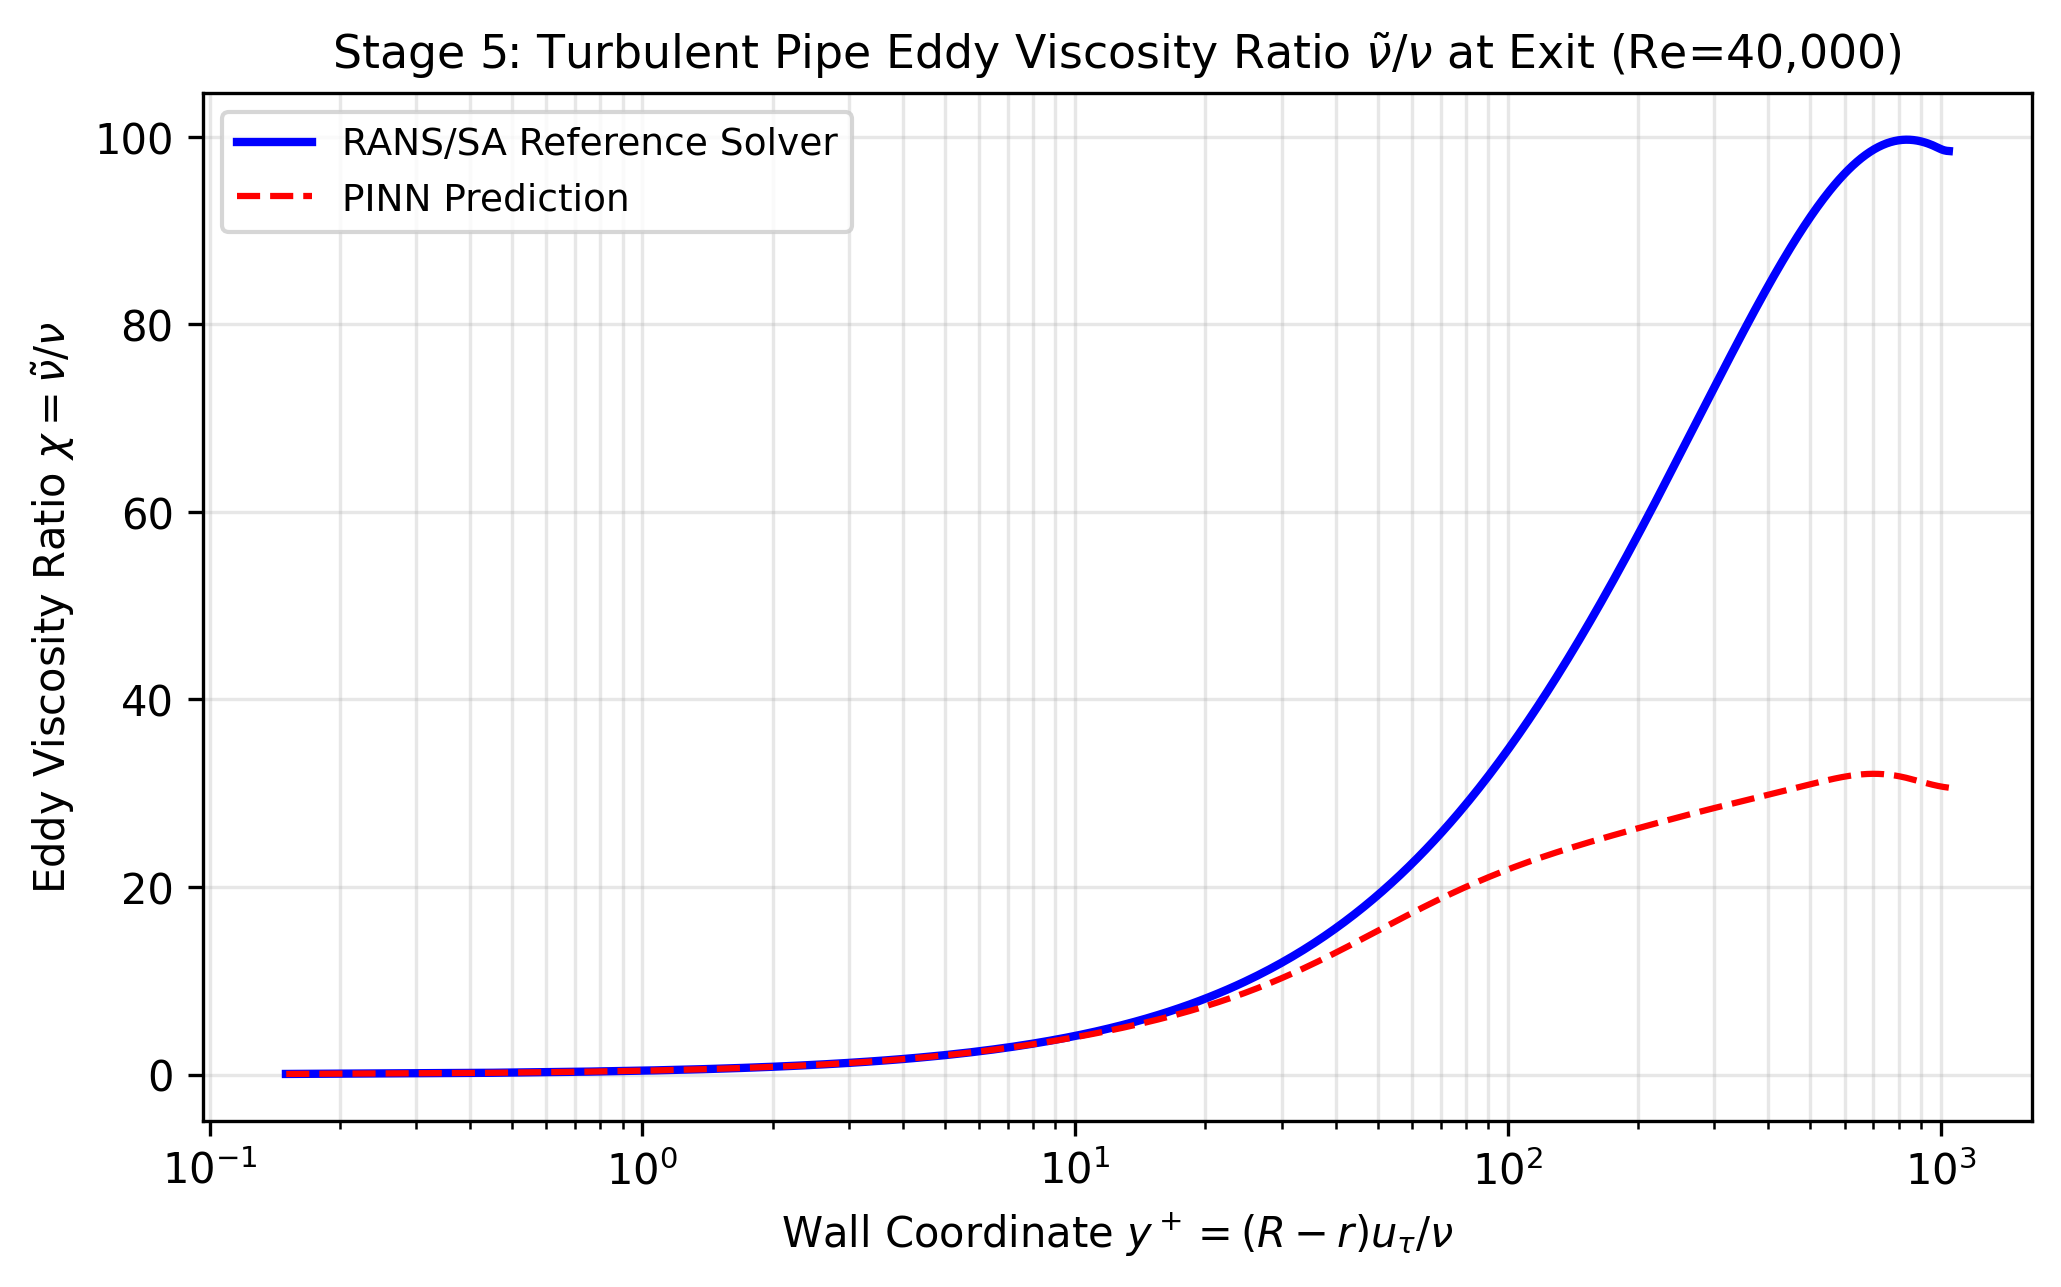
\includegraphics[width=0.85\textwidth]{stage5_nut_profiles_yplus.png}
\caption{Stage 5: Wall-normal eddy viscosity profiles $\tilde{\nu}^+(y^+)$ in pipe coordinates comparing PINN against reference.}
\label{fig:app_stage5_nut_yplus}
\end{figure}

\begin{figure}[H]
\centering
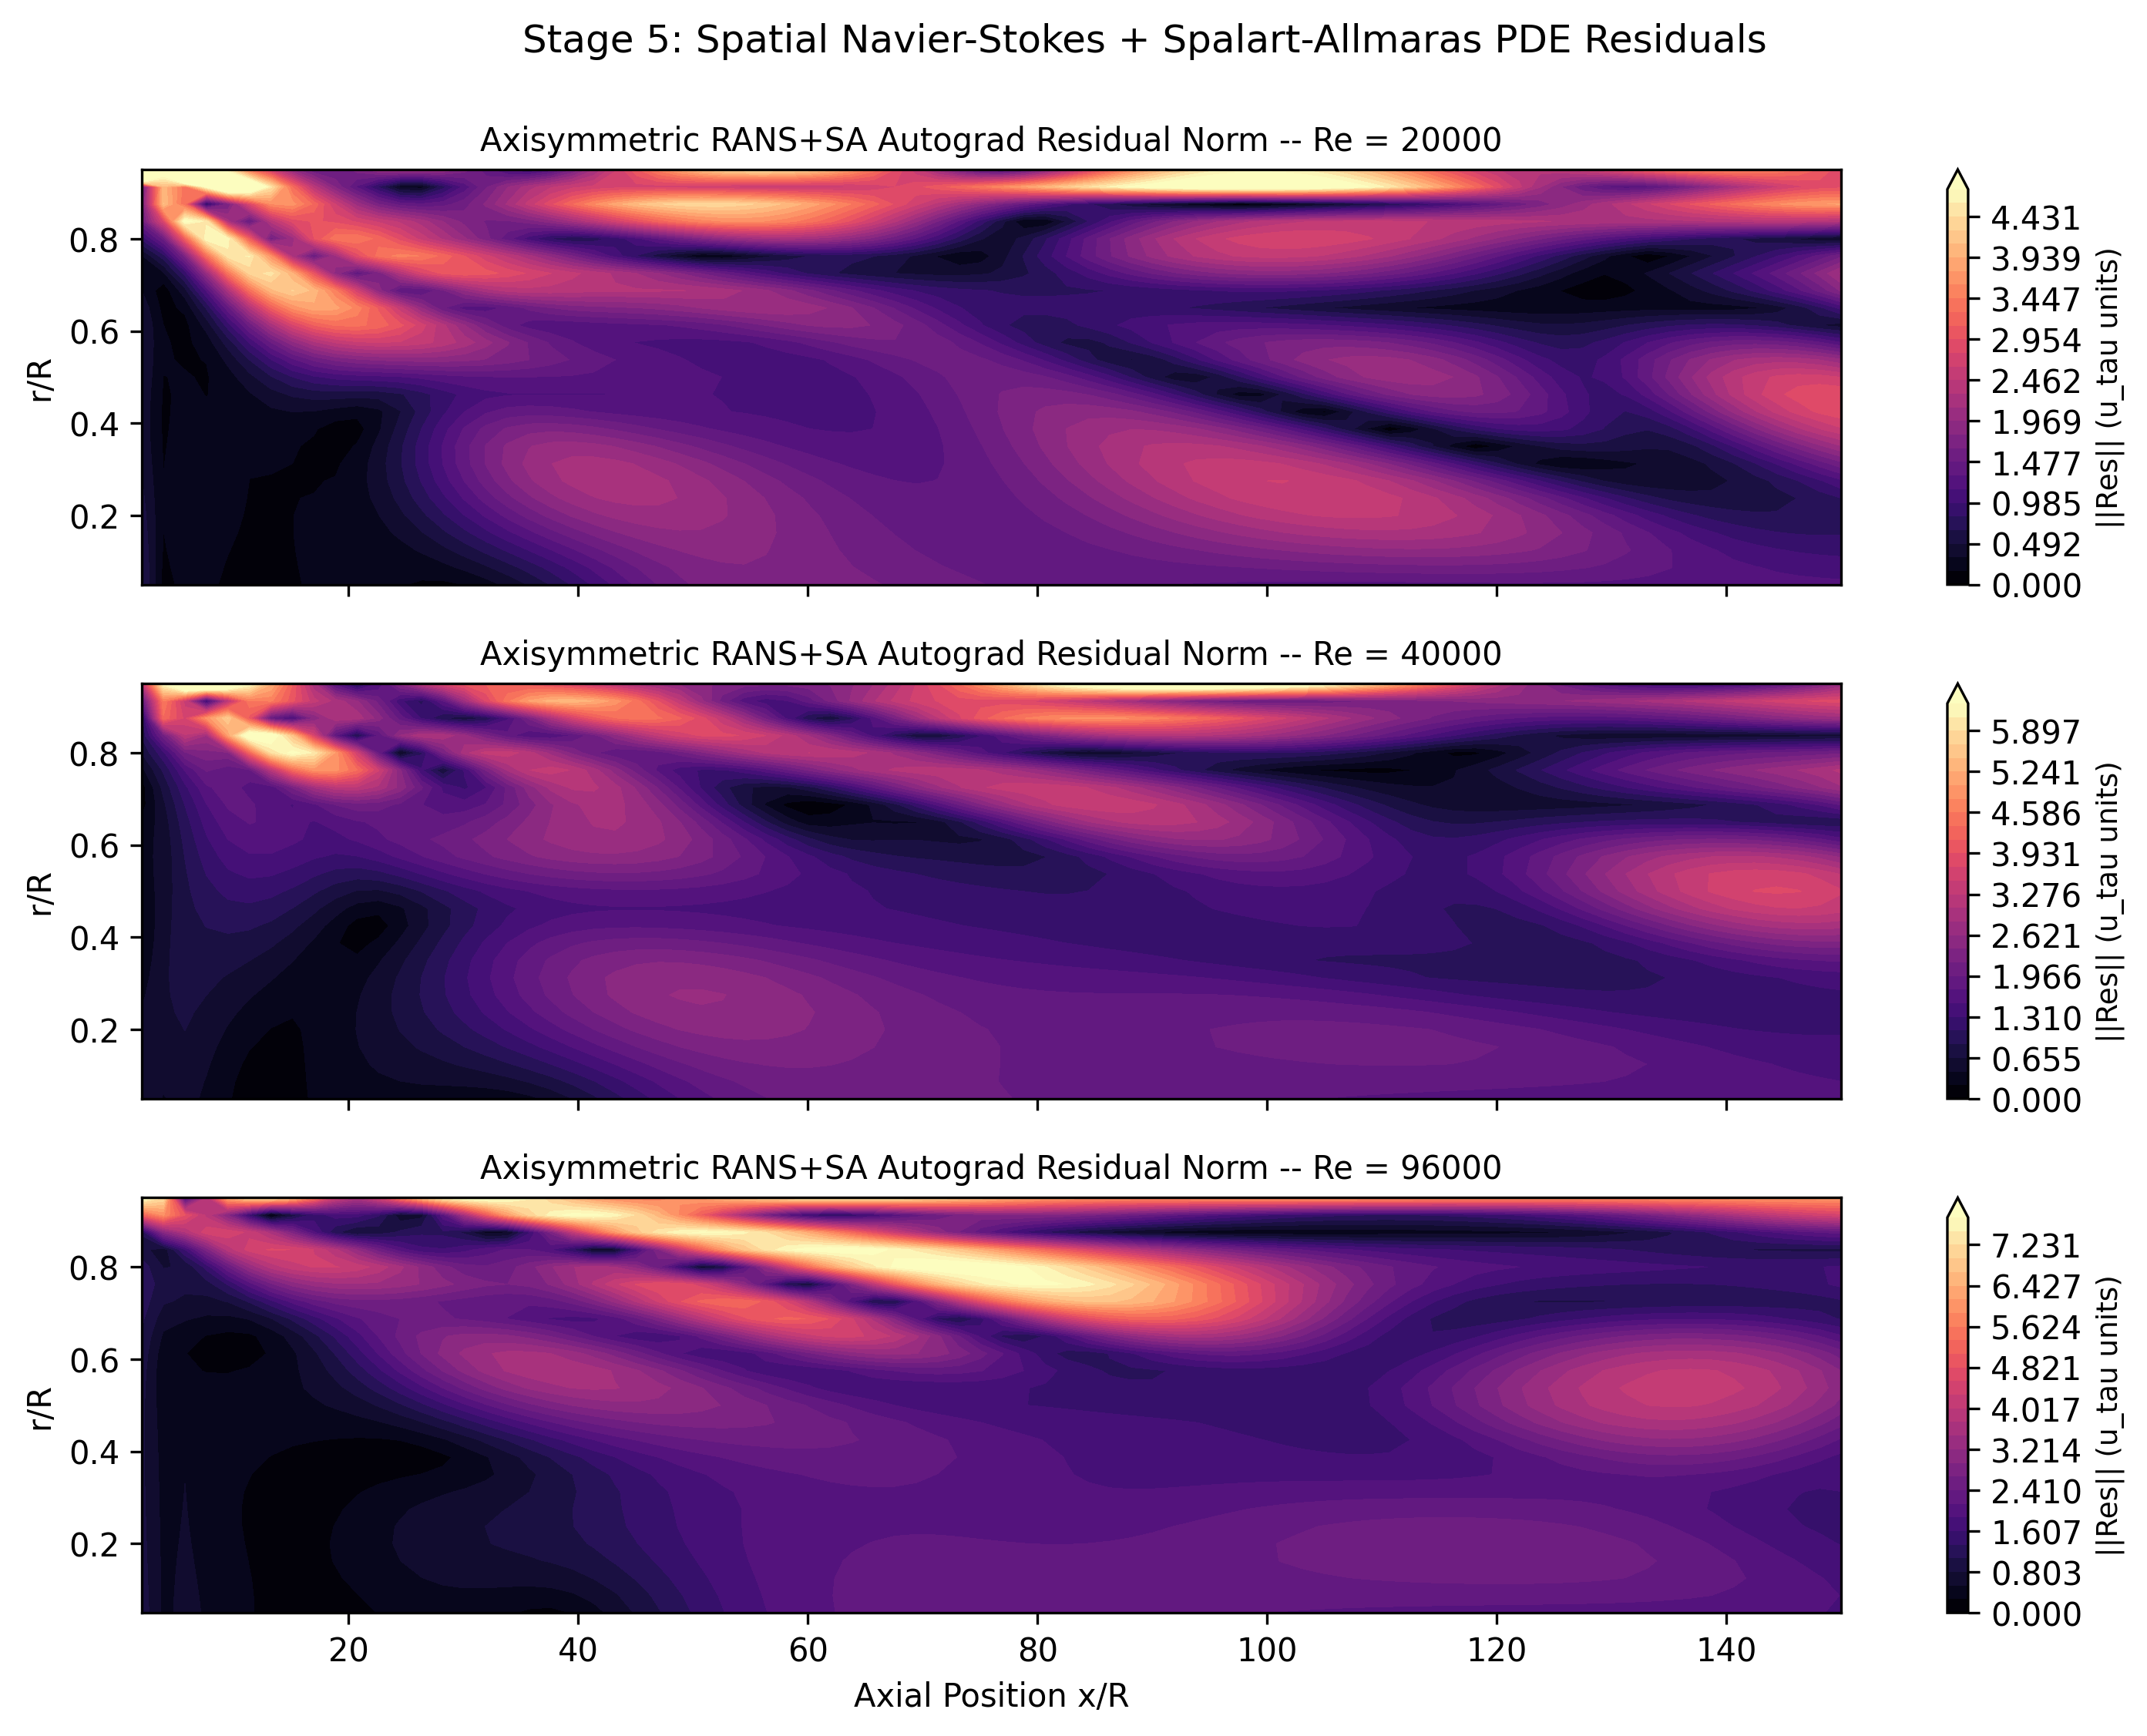
\includegraphics[width=0.85\textwidth]{stage5_residuals.png}
\caption{Stage 5: Whole-domain cylindrical RANS and SA transport residuals.}
\label{fig:app_stage5_residuals}
\end{figure}

\newpage
% ==============================================================================
% APPENDIX C: SUPPLEMENTARY TABLES
% ==============================================================================
\section{Supplementary Complete Evaluation Tables}
\label{sec:app_tables}

\subsection{Stage 4: Complete 10-Reynolds Number Evaluation Matrix}
\begin{table}[H]
\centering
\resizebox{\textwidth}{!}{
\begin{tabular}{lccccc}
\toprule
\textbf{Reynolds Number} & \textbf{Regime Split} & \textbf{Axial Velocity $u$} & \textbf{Vertical Velocity $v$} & \textbf{Kinematic Pressure $p$} & \textbf{Skin Friction $C_f$} \\
\midrule
10,000 & TRAIN & 0.69\% & 46.55\% & 0.55\% & 9.21\% \\
14,000 & VAL & 0.56\% & 33.34\% & 0.56\% & 7.90\% \\
20,000 & TRAIN & 0.47\% & 23.45\% & 0.48\% & 6.84\% \\
28,000 & TEST & 0.42\% & 16.86\% & 0.38\% & 6.11\% \\
40,000 & TRAIN & 0.39\% & 11.90\% & 0.33\% & 5.65\% \\
56,000 & VAL & 0.39\% & 8.67\% & 0.30\% & 5.42\% \\
80,000 & TRAIN & 0.43\% & 6.73\% & 0.35\% & 5.27\% \\
88,000 & VAL & 0.45\% & 6.53\% & 0.39\% & 5.25\% \\
96,000 & TEST & 0.48\% & 6.50\% & 0.44\% & 5.23\% \\
120,000 & TEST & 0.58\% & 7.14\% & 0.58\% & 5.22\% \\
\bottomrule
\end{tabular}
}
\caption{Stage 4 complete 10-Reynolds number evaluation matrix across training, validation, and test sets (Source: \texttt{4/outputs/final\_metrics.csv}). $C_f$ error is the relative error of the wall shear stress coefficient with respect to the reference solver.}
\label{tab:stage4_all_re}
\end{table}


\subsection{Stage 5: Complete 10-Reynolds Number Evaluation Matrix}
\begin{table}[H]
\centering
\resizebox{\textwidth}{!}{
\begin{tabular}{lccccc}
\toprule
\textbf{Reynolds Number} & \textbf{Regime Split} & \textbf{Axial Velocity $u$} & \textbf{Radial Velocity $v$} & \textbf{Kinematic Pressure $p$} & \textbf{Skin Friction $C_f$} \\
\midrule
10,000 & TRAIN & 0.39\% & 16.19\% & 0.25\% & 1.94\% \\
14,000 & VAL & 0.58\% & 12.28\% & 1.38\% & 2.02\% \\
20,000 & TRAIN & 0.33\% & 6.97\% & 0.19\% & 1.66\% \\
28,000 & TEST & 0.36\% & 4.69\% & 0.65\% & 1.47\% \\
40,000 & TRAIN & 0.32\% & 3.46\% & 0.17\% & 1.00\% \\
56,000 & VAL & 0.34\% & 3.20\% & 0.66\% & 0.92\% \\
80,000 & TRAIN & 0.32\% & 2.54\% & 0.16\% & 1.42\% \\
88,000 & VAL & 0.34\% & 2.58\% & 0.49\% & 1.60\% \\
96,000 & TEST & 0.38\% & 2.87\% & 0.98\% & 1.77\% \\
120,000 & TEST & 0.57\% & 4.47\% & 2.57\% & 2.24\% \\
\bottomrule
\end{tabular}
}
\caption{Stage 5 complete 10-Reynolds number evaluation matrix across training, validation, and test sets (Source: \texttt{5/outputs/eval\_dense\_final\_train+val.json} and \texttt{eval\_dense\_final\_test.json}). $C_f$ error is the relative error of the wall shear stress coefficient with respect to the reference solver.}
\label{tab:stage5_all_re}
\end{table}


\subsection{Stage 5: Princeton Superpipe Experimental Validation (All 8 Datasets)}
\begin{table}[H]
\centering
\resizebox{\textwidth}{!}{
\begin{tabular}{lccccc}
\toprule
\textbf{Experimental File} & \textbf{Experimental $\mathrm{Re}$} & \textbf{Literature Source} & \textbf{Skin Friction $C_f$} & \textbf{PINN Rel $L_2$ Error} & \textbf{Max Wall Deviation $u^+$} \\
\midrule
zag\_3.1577E+04.txt & 31,577 & Zagarola \& Smits (1998) & 0.005793 & 4.17\% & 1.46 \\
zag\_4.1727E+04.txt & 41,727 & Zagarola \& Smits (1998) & 0.005444 & 3.90\% & 1.43 \\
zag\_5.6677E+04.txt & 56,677 & Zagarola \& Smits (1998) & 0.005094 & 3.54\% & 1.35 \\
zag\_7.4293E+04.txt & 74,293 & Zagarola \& Smits (1998) & 0.004811 & 3.27\% & 1.32 \\
mck\_7.4345E+04.txt & 74,345 & McKeon et al. (2004) & 0.004811 & 3.45\% & 1.30 \\
zag\_9.8811E+04.txt & 98,811 & Zagarola \& Smits (1998) & 0.004537 & 3.02\% & 1.24 \\
mck\_1.4458E+05.txt & 144,580 & McKeon et al. (2004) & 0.004206 & 4.18\% & 1.43 \\
zag\_1.4579E+05.txt & 145,790 & Zagarola \& Smits (1998) & 0.004199 & 2.81\% & 1.15 \\
\bottomrule
\end{tabular}
}
\caption{Stage 5 Princeton Superpipe validation across all 8 experimental pitot traverse datasets (Source: \texttt{5/data/exp/} evaluated directly against \texttt{5/outputs/models/dense/final\_seed0.pt}). Literature labels are those given in the data repository~\cite{superpipe_data}. Max Wall Deviation $u^+$ is the maximum absolute pointwise deviation $\max |u^+_{\mathrm{PINN}} - u^+_{\mathrm{exp}}|$ in inner wall units ($u^+ = U/u_\tau$).}
\label{tab:superpipe_all_re}
\end{table}


\subsection{Training Configurations, Collocation Counts, and Loss Weights}
% src: 1/train_hybrid.py:119,300,398; 2/train_hybrid.py:66,262,336; 3/train_hybrid.py:147,175; 3/config.py:84,103; 4/train.py:39,139; 4/outputs/best_weights.json; 5/config.py:71; 5/outputs/best_weights_dense.json
\begin{table}[H]
\centering
\small
\resizebox{\textwidth}{!}{\begin{tabular}{lccc}
\toprule
\textbf{Training Hyperparameter} & \textbf{Stage 1 (2D Channel)} & \textbf{Stage 2 (Pipe)} & \textbf{Stage 3 (3D Duct)} \\
\midrule
Primary Optimizer & Adam (3,000 iters) & Adam (2,500 iters) & Adam (2,500 iters) \\
Polish Optimizer & L-BFGS (200 iters) & L-BFGS (300 iters) & L-BFGS (300 iters) \\
Initial Learning Rate & $8.0\times 10^{-4}$ & $8.0\times 10^{-4}$ & $8.0\times 10^{-4}$ \\
Learning Rate Schedule & StepLR ($\gamma=0.7$, step 400) & StepLR ($\gamma=0.7$, step 400) & StepLR ($\gamma=0.7$, step 500) \\
Collocation Points ($N_{\mathrm{pde}}$) & 1,500 & 1,500 & 4,000 \\
Data Points ($N_{\mathrm{data}}$) & 200 & 200 & 2,000 \\
Boundary Points ($N_{\mathrm{bc}}$) & 150 & 150 & 1,000 \\
Loss Weight Search & Grid search winner & Hand-picked baseline & Random search (20 candidates) \\
Data Loss Weight ($w_{\mathrm{data}}$) & 20.0 & 10.0 & $u: 8.73, v: 0.11, w: 11.11, p: 2.42$ \\
PDE Loss Weight ($w_{\mathrm{pde}}$) & 1.0 & 1.0 & 32.183 \\
Boundary Loss Weights & Inlet: 5.0, Wall: 5.0, Outlet: 1.0 & Inlet/Wall/Axis/Outlet: 5.0 & Inlet: 0.68, Wall: 11.14, Outlet: 0.64 \\
Relative Physics Weight & $w_{\mathrm{pde}}/w_{\mathrm{data}} = 0.05$ & $w_{\mathrm{pde}}/w_{\mathrm{data}} = 0.10$ & $w_{\mathrm{pde}}/w_{\mathrm{data},u} = 3.685$ \\
Boundary Enforcement & Soft penalty ($\mathcal{L}_{\mathrm{bc}}$) & Soft penalty ($\mathcal{L}_{\mathrm{bc}}$) & Soft penalty ($\mathcal{L}_{\mathrm{bc}}$) \\
\bottomrule
\end{tabular}}
\caption{Training configurations, collocation counts, and loss weights for laminar flow stages (Stages 1--3).}
\label{tab:training_recipes_laminar}
\end{table}

\begin{table}[H]
\centering
\small
\resizebox{\textwidth}{!}{\begin{tabular}{lcc}
\toprule
\textbf{Training Hyperparameter} & \textbf{Stage 4 (Turbulent Channel)} & \textbf{Stage 5 (Turbulent Pipe)} \\
\midrule
Primary Optimizer & Adam (12,000 iters) & Adam (12,000 iters) \\
Polish Optimizer & L-BFGS (200 iters) & L-BFGS (200 iters) \\
Initial Learning Rate & $4.37\times 10^{-3}$ & $8.40\times 10^{-3}$ \\
Learning Rate Schedule & ExponentialLR ($100\times$ decay) & ExponentialLR ($100\times$ decay) \\
Collocation Points ($N_{\mathrm{pde}}$) & 2,048 & 2,048 \\
Data Points ($N_{\mathrm{data}}$) & 2,048 & 2,048 \\
Boundary Points ($N_{\mathrm{bc}}$) & 512 & 512 \\
Loss Weight Search & Optuna TPE (44 trials) & Optuna TPE (48 trials) \\
Data Loss Weight ($w_{\mathrm{data}}$) & 6,768.755 & 1,996.576 \\
PDE Loss Weight ($w_{\mathrm{pde}}$) & Mom: $3.436\times 10^{-5}$, SA: $3.307\times 10^{-5}$ & Mom: $5.519\times 10^{-4}$, SA: 2.2332 \\
Boundary Loss Weights & Inlet: 0.120, Outlet: 5.525, Sym: 1.324 & Inlet: 1.515, Outlet: 2.055, Sym: 0.359 \\
Relative Momentum Weight ($w_{\mathrm{mom}}/w_{\mathrm{data}}$) & $5.08\times 10^{-9}$ & $2.76\times 10^{-7}$ \\
Relative SA Weight ($w_{\mathrm{sa}}/w_{\mathrm{data}}$) & $4.89\times 10^{-9}$ & $1.12\times 10^{-3}$ \\
Boundary Enforcement & Hard $\tanh$ envelope & Hard $\tanh$ envelope \\
\bottomrule
\end{tabular}}
\caption{Training configurations, collocation counts, and loss weights for turbulent RANS+SA stages (Stages 4--5).}
\label{tab:training_recipes_turb}
\end{table}


\subsection{Stage 3: Centerline Pressure Drop Mismatch Across Reynolds Numbers}
% src: tools/dp_ratio.py
\begin{table}[H]
\centering
\small
\resizebox{\textwidth}{!}{
\begin{tabular}{ccccccc}
\toprule
$\mathrm{Re}$ & $\Delta p_{\mathrm{ref}}$ [$\mathrm{m^2/s^2}$] & $\Delta p_{\mathrm{PINN}}$ [$\mathrm{m^2/s^2}$] & $\left.\frac{dp}{dx}\right|_{\mathrm{ref}}$ [$\mathrm{m/s^2}$] & $\left.\frac{dp}{dx}\right|_{\mathrm{PINN}}$ [$\mathrm{m/s^2}$] & $\left.\frac{dp}{dx}\right|_{\mathrm{ana}}$ [$\mathrm{m/s^2}$] & $\frac{\mathrm{slope}_{\mathrm{PINN}}}{\mathrm{slope}_{\mathrm{ref}}}$ \\
\midrule
50  & $+1.948\times 10^{-1}$ & $-6.617\times 10^{-3}$ & $-6.564\times 10^{-3}$ & $-1.429\times 10^{-3}$ & $-6.560\times 10^{-3}$ & $0.22\times$ \\
100 & $+3.618\times 10^{-1}$ & $-2.240\times 10^{-2}$ & $-1.285\times 10^{-2}$ & $-4.851\times 10^{-3}$ & $-1.312\times 10^{-2}$ & $0.38\times$ \\
200 & $+6.113\times 10^{-1}$ & $-6.849\times 10^{-2}$ & $-2.322\times 10^{-2}$ & $-1.486\times 10^{-2}$ & $-2.624\times 10^{-2}$ & $0.64\times$ \\
300 & $+7.887\times 10^{-1}$ & $-1.249\times 10^{-1}$ & $-3.255\times 10^{-2}$ & $-2.708\times 10^{-2}$ & $-3.936\times 10^{-2}$ & $0.83\times$ \\
500 & $+1.002\times 10^{0}$  & $-2.506\times 10^{-1}$ & $-5.342\times 10^{-2}$ & $-5.398\times 10^{-2}$ & $-6.560\times 10^{-2}$ & $1.01\times$ \\
600 & $+1.056\times 10^{0}$  & $-3.154\times 10^{-1}$ & $-6.526\times 10^{-2}$ & $-6.760\times 10^{-2}$ & $-7.872\times 10^{-2}$ & $1.04\times$ \\
\bottomrule
\end{tabular}
}
\par\vspace{0.4em}\noindent\textit{Note:} Over $x=0.05\,\text{m}$ to $5.0\,\text{m}$, the reference pressure first rises (inlet transient, $x < 0.5\,\text{m}$), so $\Delta p_{\mathrm{ref}} = p(5.0) - p(0.05)$ is dominated by that transient; the PINN pressure falls monotonically ($\Delta p_{\mathrm{PINN}} < 0$). In the downstream window ($x \in [1.5, 5.0]\,\text{m}$), both pressures fall downstream, with $\mathrm{slope}_{\mathrm{PINN}}/\mathrm{slope}_{\mathrm{ref}} = 0.22$ to $1.04$ of the reference slope ($0.38$ at $\mathrm{Re}=100$, matching within $4\%$ for $\mathrm{Re} \ge 500$). For $\mathrm{Re} \ge 200$ the reference slope is $11\%$--$19\%$ below the analytic fully developed value, so the window is not fully developed there.
\caption{Stage 3 centerline pressure development: full-domain difference $\Delta p = p(5.0) - p(0.05)$ and downstream pressure gradients $dp/dx$ in the downstream window ($x \in [1.5, 5.0]\,\text{m}$) along $(y=H/2, z=W/2)$, where $\left.\frac{dp}{dx}\right|_{\mathrm{ana}}$ denotes the analytic fully developed gradient ($f\cdot\mathrm{Re}=62.196$).}
\label{tab:stage3_dp_ratio}
\end{table}

\begin{figure}[H]
\centering
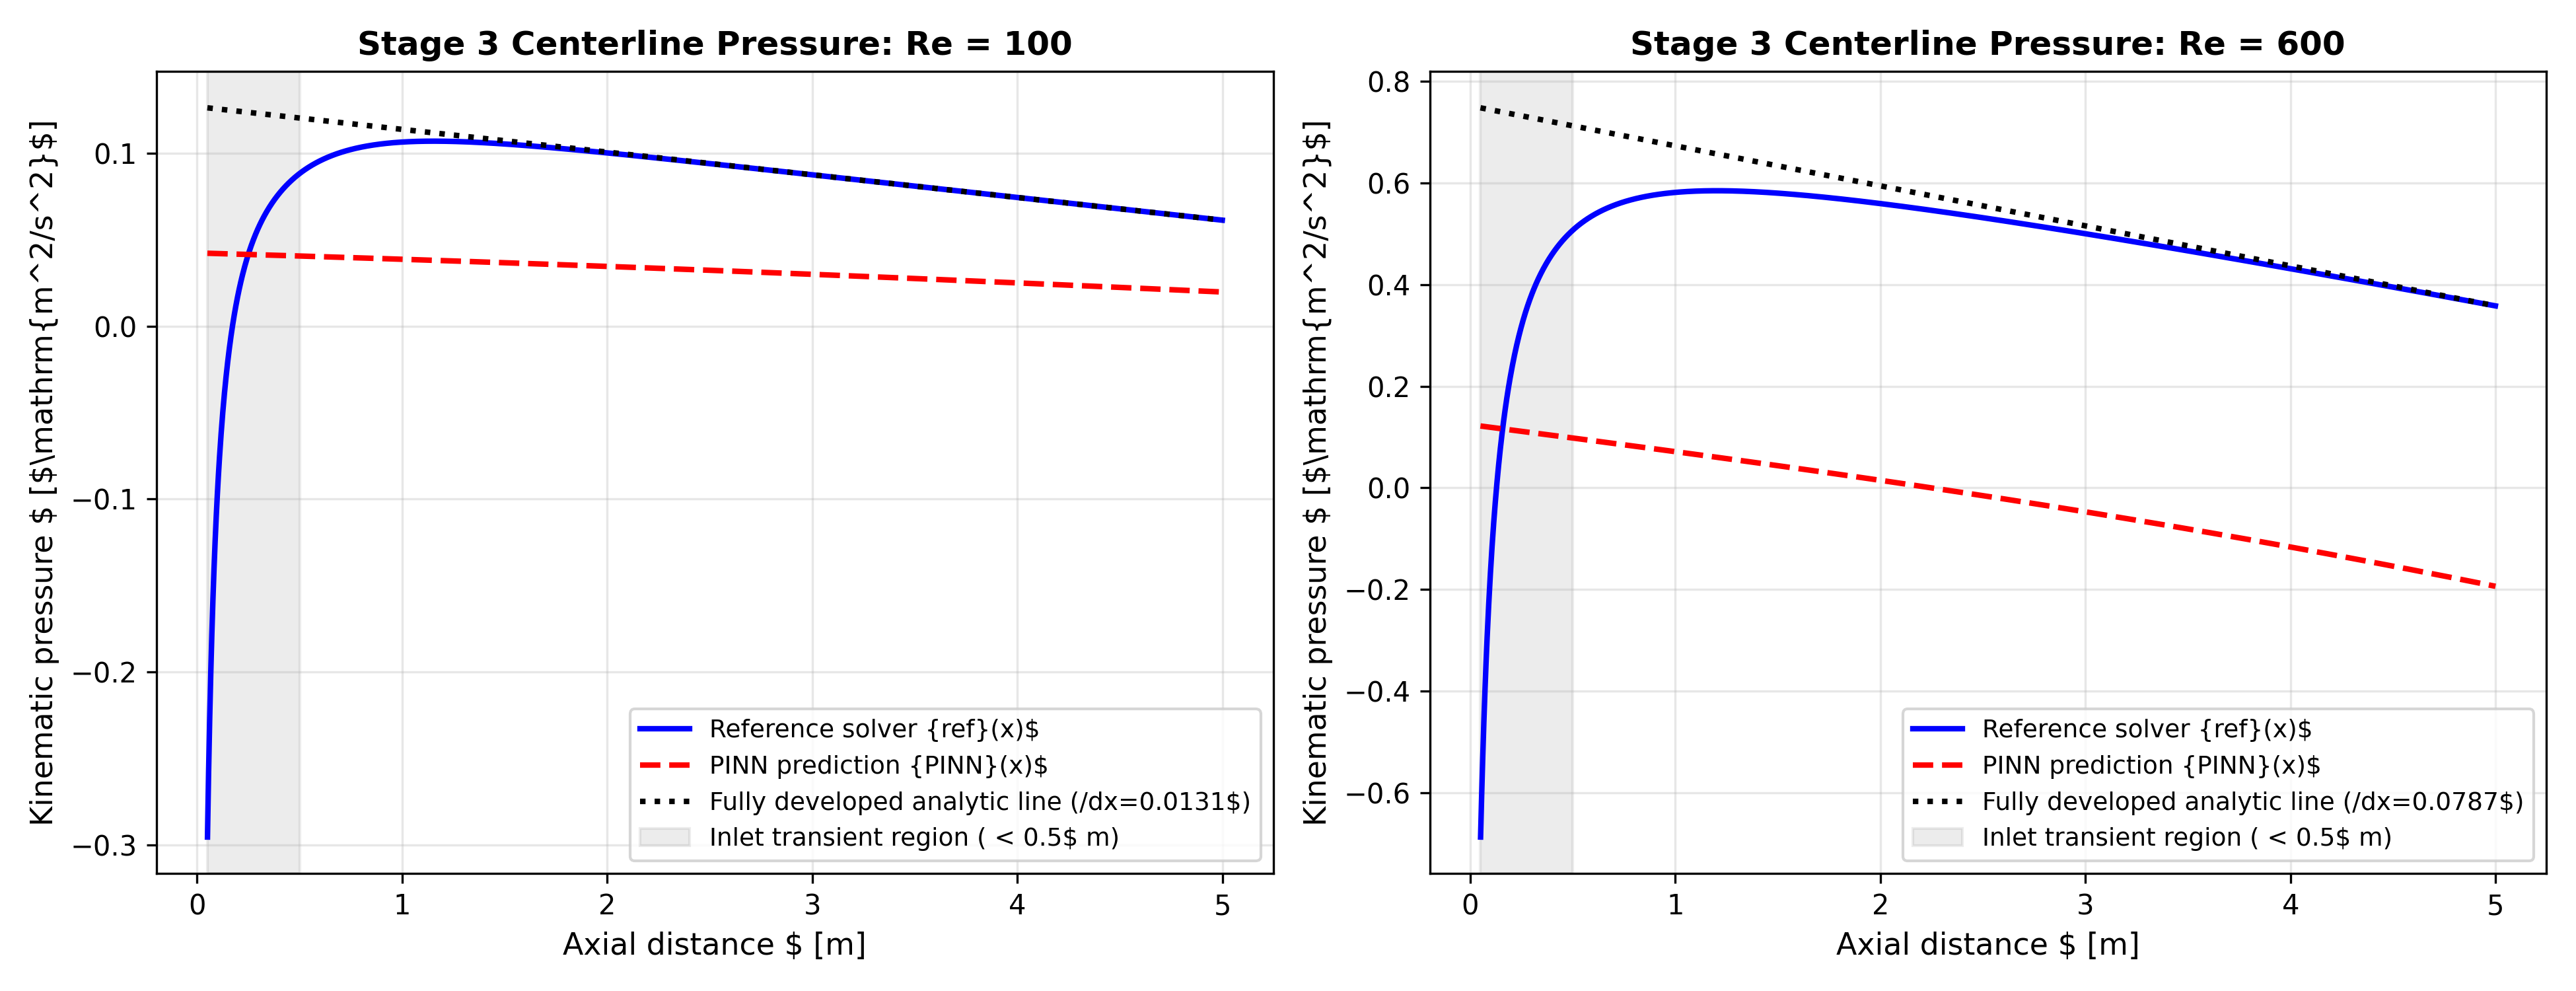
\includegraphics[width=0.88\textwidth]{stage3_centerline_p.png}
\caption{Stage 3: Centerline kinematic pressure development $p(x)$ at $\mathrm{Re}=100$ (left) and $\mathrm{Re}=600$ (right) along $(y=H/2, z=W/2)$, comparing reference marching solver, PINN prediction, and the theoretical fully developed Darcy gradient ($f\cdot\mathrm{Re}=62.196$). Most of the reference variation occurs in the inlet transient region of the reference solution (cause not isolated) ($x < 0.5\,\mathrm{m}$).}
\label{fig:stage3_centerline_p_analytic}
\end{figure}


\paragraph{Code and Data Availability.}
Production checkpoints are stored at \path{1/outputs/channel_pinn_hybrid.pt}, \path{2/checkpoints/pipe_pinn.pt}, \path{3/checkpoints/duct_pinn.pt}, \path{4/models/best.pt} and \path{5/outputs/models/dense/final_seed0.pt}. Reference data generation routines reside in stage directories (\path{1/entrance_solver.py}, \path{2/entrance_solver.py}, \path{3/duct_solver.py}, \path{4/build_reference.py}, and \path{5/build_reference.py}). Global diagnostic visualizations and tabular syntheses are generated by \path{generate_all_plots.py}, prediction flow fields by \path{tools/plot_predictions.py}, loss breakdown calculations by \path{tools/compute_weighted_losses.py}, and pressure gradient metrics by \path{tools/dp_ratio.py}. 



\section{Design Choices and Their Basis}
\label{sec:appendix_design_choices}
Table~\ref{tab:design_choices_registry} lists the design choices and, for each, the source or the reason.

\begin{table}[H]
\centering
\small
\resizebox{\textwidth}{!}{
\begin{tabular}{lp{5.5cm}p{10.0cm}}
\toprule
\textbf{Design Item} & \textbf{Adopted Value / Configuration} & \textbf{Basis and Justification} \\
\midrule
Network Depth and Width (Stages 1--3) & 4 hidden layers, width 80 (20,003 parameters) & Selected empirically. \\
Network Depth and Width (Stages 4--5) & 4 hidden layers, width 64 (13,060 parameters) & Selected empirically. \\
Activation Function & Hyperbolic tangent ($\tanh$) & Authors' choice: infinitely differentiable ($C^\infty$) activation function required to evaluate non-vanishing and continuous second-order viscous diffusion derivatives ($\nabla^2 u$). \\
Weight Initialization & Xavier normal, zero bias & Glorot and Bengio~\cite[Eq.~(12), p.~253]{glorot2010}: maintains constant activation and backpropagated gradient variance across layers for symmetric activations with unit derivative at zero ($f'(0)=1$). \\
Input Coordinate Scaling & $\hat{x} = x/L$, $\hat{y} = y/H$, $\hat{r} = r/R$, $\hat{z} = z/W \in [-1, 1]$ & Selected empirically. \\
Reynolds Number Embedding & $\mathrm{Re}_n = 2\frac{\log_{10}\mathrm{Re} - \log_{10}\mathrm{Re}_{\min}}{\log_{10}\mathrm{Re}_{\max} - \log_{10}\mathrm{Re}_{\min}} - 1$ & Authors' choice: logarithmic scaling spaces operating conditions evenly across decades ($\mathrm{Re} \in [50, 600]$ or $[10^4, 1.2\times 10^5]$). \\
Dimensionless Output Scaling & $u/U_{\mathrm{ref}}$, $v/U_{\mathrm{ref}}$, $p/p_{\mathrm{scale}}$ & Authors' choice: rescales network outputs to order $\mathcal{O}(1)$ across all operating Reynolds numbers. \\
Hard Boundary Envelope & $g = \tanh(\mathrm{Re}_\tau \eta / 10)$ with constant 10 & Authors' choice: scaling constant 10 ensures $g = \tanh(2.0) \approx 0.964$ at $y^+ = 20$, strictly enforcing zero no-slip wall conditions while leaving buffer and log layers unconstrained. \\
Transverse Velocity Scale & $v_s = 0.05\,\sqrt{0.5 \times 0.073\,(\mathrm{Re}/2)^{-0.25}}$ & Selected empirically. \\
Softplus Working Variable Offset & $\tilde{\nu} \propto \operatorname{softplus}(\cdot - 3.0)$ & Authors' choice: softplus guarantees non-negative eddy viscosity $\tilde{\nu} \ge 0$; offset $-3.0$ establishes initial baseline $\ln(1+e^{-3}) \approx 0.0486$. \\
Collocation and Data Budgets (Stages 1--2) & $N_{\mathrm{data}} = 200$, $N_{\mathrm{pde}} = 1,500$, $N_{\mathrm{bc}} = 150$ & Selected empirically. \\
Collocation and Data Budgets (Stage 3) & $N_{\mathrm{data}} = 2,000$, $N_{\mathrm{pde}} = 4,000$, $N_{\mathrm{bc}} = 1,000$ & Selected empirically. \\
Collocation and Data Budgets (Stages 4--5) & $N_{\mathrm{data}} = 2,048$, $N_{\mathrm{pde}} = 2,048$, $N_{\mathrm{bc}} = 512$ & Selected empirically. \\
Primary Optimizer & Adam (2,500--3,000 iters laminar; 12,000 iters turbulent) & Adam~\cite[Sec.~2, Algorithm~1, p.~2]{kingma2015}; used before L-BFGS following Rao et al.~\cite[Sec.~3.1, p.~3]{rao2020}. \\
Polish Optimizer & L-BFGS (200--300 iters) & Raissi et al.~\cite[Sec.~2.1, p.~6]{raissi2019}: used L-BFGS for the fine optimization phase. \\
Learning Rate Schedules & StepLR ($\gamma=0.7$, 400--500 steps) and ExponentialLR & Selected empirically. \\
Loss Weight Discovery & Grid search (Stage 1), Hand-tuned (Stage 2), Random (Stage 3), Optuna (Stages 4--5) & Selected empirically per stage: grid search (Stage 1), hand-tuned (Stage 2), random search over 20 candidates (Stage 3), Optuna TPE over 44 trials (Stage 4) and 48 trials (Stage 5); see Tables~\ref{tab:training_recipes_laminar}--\ref{tab:training_recipes_turb}. \\
Conduit Domain Lengths & $L = 4.0\,\text{m}$ (Stages 1--2), $5.0\,\text{m}$ (Stage 3), $L/h = 160$ (Stages 4--5) & Authors' choice: sized so that laminar entrance development length ($L_e = 1.33\,\text{m}$ for channel, $3.41\,\text{m}$ for pipe at $\mathrm{Re}=600$) fits within the domain. \\
Reynolds Number Operating Sweeps & $\mathrm{Re} \in [50, 600]$ (Stages 1--3), $\mathrm{Re} \in [10^4, 1.2\times 10^5]$ (Stages 4--5) & Selected empirically. \\
Reynolds Number Splits & See Table~\ref{tab:reynolds_splits} & Documented in Section~\ref{sec:reynolds_splits}. \\
Turbulent Shear Velocity Estimate & $u_\tau = \sqrt{0.5 \times 0.0791\,\mathrm{Re}^{-0.25}}$ (pipe), $0.073$ (channel) & Blasius-type estimate $u_\tau=\sqrt{0.5\times0.0791\,\mathrm{Re}^{-0.25}}$ (pipe), Dean-type $0.073\,\mathrm{Re}^{-0.25}$ (channel); used only to scale the envelope and the features. \\
Friction Velocity Reynolds Scaling & $\mathrm{Re}_\tau = 0.0955\,(\mathrm{Re}/2)^{0.875}$ & Authors' choice: this power law reproduces the $\mathrm{Re}_\tau \in \{180, 395, 590\}$ DNS cases of Moser et al.~\cite{moser1999} within 2.2\%. \\
Spalart--Allmaras Closure Constants & $c_{b1}=0.1355, \sigma=2/3, c_{b2}=0.622, \kappa=0.41, c_{w2}=0.3, c_{w3}=2.0, c_{v1}=7.1$ & Allmaras et al.~\cite[Sec.~2.1, p.~2]{allmaras2012}: standard calibrated closure coefficients of the baseline Spalart--Allmaras model. \\
Laminar Entrance Length Correlation & $L_e/D_h = [(0.3155)^{1.6} + (0.01105\,\mathrm{Re})^{1.6}]^{1/1.6}$ (channel), $[(0.619)^{1.6} + (0.0567\,\mathrm{Re})^{1.6}]^{1/1.6}$ (pipe) & Ray et al.~\cite[Eqs.~(2a)--(2b), p.~8]{ray2017}: empirical correlations reproducing the numerical investigations of Durst et al. \\
Turbulent Pipe Friction Benchmark & $1/\lambda^{1/2} = A \log_{10}(\mathrm{Re}_b \lambda^{1/2}) - B$ & Pirozzoli et al.~\cite[Eq.~(3.2), p.~7]{pirozzoli2021}: Prandtl friction law with DNS fit constants $A \approx 2.102, B \approx 1.148$. Empirical benchmark. \\
Turbulent Channel Skin Friction Correlation & Dean's correlation $C_f = 0.073\,(\mathrm{Re}/2)^{-0.25}$ & Empirical benchmark. \\
Profile Stations in Figures & $x = 0.243, 0.670, 1.325\,\text{m}$ & Authors' choice: entrance lengths of an Atkinson-type correlation; within 1.7\% of [6] at $\mathrm{Re}=100$ and 0.5\% at $\mathrm{Re}=600$. \\
Reynolds Number Definitions & $U_0 D_h/\nu$ (channel), $U_0 D/\nu$ (pipe), $U_b D_h/\nu$ (duct) & Standard internal flow definitions tabulated in Table~\ref{tab:reynolds_splits}. \\
Collocation and Data Sampling & Fresh sampling every Adam step ($N_{\mathrm{data}}, N_{\mathrm{pde}}, N_{\mathrm{bc}}$) & Fresh random sampling at every Adam iteration (training code). \\
Relative $L_2$ Error Metric & $E_f = \|f_{\mathrm{PINN}} - f_{\mathrm{ref}}\|_2 / \|f_{\mathrm{ref}}\|_2$ & Standard evaluation metric defined in Section~\ref{sec:error_metrics}. \\
\bottomrule
\end{tabular}}
\caption{Register of design choices, hyperparameter values, and their scientific basis across Stages 1--5.}
\label{tab:design_choices_registry}
\end{table}


\end{document}
